\documentclass[11pt,a4paper,oldfontcommands]{memoir}
\hfuzz=2.1pt 
\usepackage[
breaklinks=true,colorlinks=true,
linkcolor=blue,urlcolor=blue,citecolor=blue,% PDF VIEW
%linkcolor=black,urlcolor=black,citecolor=black,% PRINT
bookmarks=true,bookmarksopenlevel=2]{hyperref}
\setlength{\headheight}{27.3pt}
\raggedbottom
\usepackage[utf8]{inputenc}
\usepackage[T1]{fontenc}
\usepackage{microtype}
\usepackage[dvips]{graphicx}
\usepackage{xcolor}
\usepackage{times}
\usepackage[brazilian]{babel}
\usepackage{indentfirst}
\usepackage{multirow}
\usepackage{caption}
\usepackage{courier}
\usepackage{longtable}
\usepackage{float}
\restylefloat{table}
\ifpdf
	\usepackage{pdfcolmk}
\fi
\pdfminorversion=7
\newlength{\drop}% for my convenience
\newcommand*{\plogo}{%\fbox
	{$\mathcal{GPMCP}$}}
\makeatletter

\usepackage{geometry}
% PDF VIEW
\geometry{
	%total={210mm,297mm}, 
	left=22mm,
	right=23mm,
	bindingoffset=0mm, 
	top=25mm,bottom=25mm
	}
% PRINT
% \geometry{
	% total={210mm,297mm},
	% left=20mm,
	% right=20mm,
	% bindingoffset=10mm, 
	% top=25mm,bottom=25mm
	% }

\usepackage{array}
\usepackage{tikz}
\usetikzlibrary{calc,trees,positioning,arrows,chains,shapes.geometric,%
    decorations.pathreplacing,decorations.pathmorphing,shapes,%
    matrix,shapes.symbols,shapes.arrows}

\tikzset{
>=stealth',
  punktchain/.style={
    rectangle, 
    rounded corners, 
    % fill=black!10,
    draw=black, very thick,
    text width=10em, 
    minimum height=3em, 
    text centered, 
    on chain},
  line/.style={draw, thick, <-},
  element/.style={
    tape,
    top color=white,
    bottom color=blue!50!black!60!,
    minimum width=10em,
    draw=blue!40!black!90, very thick,
    text width=10em, 
    minimum height=3.5em, 
    text centered, 
    on chain},
  every join/.style={->, thick,shorten >=1pt},
  decoration={brace},
  tuborg/.style={decorate},
  tubnode/.style={midway, right=2pt},
}
\tikzset{
>=stealth',
  pequeno/.style={
    rectangle, 
    rounded corners, 
    % fill=black!10,
    draw=black, very thick,
    text width=2em, 
    minimum height=3em, 
    text centered, 
    on chain},
  line/.style={draw, thick, <-},
  element/.style={
    tape,
    top color=white,
    bottom color=blue!50!black!60!,
    minimum width=2em,
    draw=blue!40!black!90, very thick,
    text width=2em, 
    minimum height=3.5em, 
    text centered, 
    on chain},
  every join/.style={->, thick,shorten >=1pt},
  decoration={brace},
  tuborg/.style={decorate},
  tubnode/.style={midway, right=2pt},
}
\tikzset{
>=stealth',
  grande/.style={
    rectangle, 
    rounded corners, 
    % fill=black!10,
    draw=black, very thick,
    text width=20em, 
    minimum height=3em, 
    text centered, 
    on chain},
  line/.style={draw, thick, <-},
  element/.style={
    tape,
    top color=white,
    bottom color=blue!50!black!60!,
    minimum width=20em,
    draw=blue!40!black!90, very thick,
    text width=20em, 
    minimum height=3.5em, 
    text centered, 
    on chain},
  every join/.style={->, thick,shorten >=1pt},
  decoration={brace},
  tuborg/.style={decorate},
  tubnode/.style={midway, right=2pt},
}
\OnehalfSpacing
%\linespread{1.3}

%%% CHAPTER'S STYLE
\chapterstyle{bianchi}
%\chapterstyle{ger}
%\chapterstyle{madsen}
%\chapterstyle{ell}
%%% STYLE OF SECTIONS, SUBSECTIONS, AND SUBSUBSECTIONS
\setsecheadstyle{\Large\bfseries\sffamily\raggedright}
\setsubsecheadstyle{\large\bfseries\sffamily\raggedright}
\setsubsubsecheadstyle{\bfseries\sffamily\raggedright}


%%% STYLE OF PAGES NUMBERING
%\pagestyle{companion}\nouppercaseheads
%\pagestyle{headings}
%\pagestyle{Ruled}
%\pagestyle{plain}
%\makepagestyle{plain}
\copypagestyle{chapter}{plain}
\makeevenfoot{chapter}{\thepage}{}{}
\makeoddfoot{chapter}{}{}{\thepage}
\makeevenfoot{headings}{\thepage}{}{CC-BY 4.0 FHC Felix 2014-2019}
\makeoddfoot{headings}{CC-BY 4.0 FHC Felix 2014-2019}{}{\thepage}
\makeevenhead{plain}{}{}{}
\makeoddhead{plain}{}{}{}

\maxsecnumdepth{subsection} % chapters, sections, and subsections are numbered
\maxtocdepth{subsection} % chapters, sections, and subsections are in the Table of Contents

\newenvironment{dedication}
	{
	\cleardoublepage
	\thispagestyle{empty}
	\vspace*{\stretch{3}}
	\hfill
		\begin{minipage}[t]{0.66\textwidth}
		\raggedright
		\end{minipage}
	\vspace*{\stretch{1}}
	\clearpage
	}

\makeatletter
\renewcommand{\@chapapp}{}% Not necessary...
\newenvironment{chapquote}[2][2em]
	{\setlength{\@tempdima}{#1}%
	\def\chapquote@author{#2}%
	\parshape 1 \@tempdima \dimexpr\textwidth-2\@tempdima\relax%
	\itshape}
{\par\normalfont\hfill--\ \chapquote@author\hspace*{\@tempdima}\par\bigskip}
\makeatother

\newcommand*{\titleGP}
	{\begingroup % Geometric Modeling
		\drop=0.1\textheight
		\raggedright
			\vspace*{\baselineskip}
			\rule{\textwidth}{1.6pt}\vspace*{-\baselineskip}\vspace*{2pt}
			\rule{\textwidth}{0.4pt}\\[\baselineskip]
			{\HUGE PROTOCOLOS DE QUIMIOTERAPIA \\[0.5\baselineskip]}
			%\rule{\textwidth}{0.4pt}\vspace*{-\baselineskip}\vspace{3.2pt}
			\rule{\textwidth}{1.6pt}\\[\baselineskip]
			\scshape
			\large Manual de tratamento clínico de pacientes pediátricos \break com tumores cerebrais
			\vfill
			\par
		\raggedleft
			{\Large \textsc{FHC Félix}}
			\par
			%\plogo
			{\scshape 2019}
			%{\large Editoração própria}
			\par
	\endgroup}

\newcommand*{\titleM}
	{\begingroup % Geometric Modeling
		\drop=0.1\textheight
		\centering
			\vspace*{\baselineskip}
			{\LARGE PROTOCOLOS DE QUIMIOTERAPIA 
			\\[0.5\baselineskip]}
			\scshape
			{\Large Manual de
			tratamento clínico de pacientes pediátricos com tumores cerebrais \\[0.5\baselineskip]}\par
			\vfill
			{\Large \textit{Editado por}} \\
			[\baselineskip]\par
			{\Large FRANCISCO H. C. FÉLIX \par}
			{\itshape Centro Pediátrico do Câncer, Hospital Infantil Albert Sabin \par}
			{\Large JUVENIA B. FONTENELE \par}
			{\itshape Faculdade de Farmácia, Odontologia e Enfermagem,
			Universidade Federal do Ceará - Fortaleza - CE\par}
			\vspace*{4\baselineskip}
			%{\Large \textit{Prefácio de}
			% \textsc{Nádia M. Trompieri}}
			\vfill
			{\scshape 2019}
			{\large Github\par}
			{\itshape \small http://bit.ly/fhcflx1p\par}
	\endgroup}

\def\contributors{\chapter*{COLABORADORES}
	\vskip1sp
	\leftskip=10pt
	\parindent-10pt
	\vskip-2pt
	\everypar={}
	\def\footnote##1{\hskip-10pt\savefootnote{##1}\hskip10pt}
	\setcounter{page}{5}
	%\global\titletrue
	\markboth{COLABORADORES}{COLABORADORES}
	}

\def\endcontributors{\newpage\markboth{}{}}

\def\name#1{\vskip2pt\fakesc #1*\hskip10pt}

\def\timesroman{cmr10 }
\def\timesbold{cmbx10 }
\def\timesitalic{cmti10 }
\def\timesbolditalic{cmbx10 }
\font\bigscfont\timesroman at 11.5pt
\font\smscfont\timesroman at 9.5pt
\font\wherefont\timesitalic at 10pt

\def\fakesc#1*{\edef\stuff{#1 }%
	\expandafter\pickupnewword\stuff* }
\def\saveast{*}

\def\rrelax{\relax}

\def\pickupnewlett#1{\def\letter{#1}%
	\ifx\letter\saveast\unskip%
	\let\go\relax \else%
	\ifx\letter\rrelax{\bigscfont\ }%
	\let\go\pickupnewword\else%
	\uppercase{\def\ucletter{#1}%  upper case letter
	\ifx\letter\ucletter%
	{\bigscfont#1}\else{\smscfont#1}\fi}%%
	\let\go\pickupnewlett\fi\fi\go
	}

\def\pickupnewword#1 {\expandafter\pickupnewlett#1\relax}

%\def\halftitlepage{\thispagestyle{empty}
%	\vspace*{9pc}%
%		{\parindent \z@
%			\interlinepenalty\@M
%		\LARGE
%		\hyphenpenalty10000
%		\bfseries\halftitlefont
%		\def\\ {\vskip 1sp}
%		\noindent\thetitle\vskip 1sp
%		}
%	\newpage
%	}

%\def\affil#1{{\affilfont #1}\vskip18pt}

%\def\dotspace{\hskip5pt/\hskip5pt}

\def\entrywithlabel[#1]#2{\parbox{#1}{{\small #2:} \hrulefill}}
\def\entrywithlabelunder[#1]#2{\parbox{#1}{\hrulefill\\[-.75ex]\centerline {#2}}}
\def\entrywithlabelraised[#1]#2{\parbox{#1}{\smash{\raise-1ex\hbox{{\tiny #2}}}\hrulefill}}
\def\boxentry[#1]#2{{\setlength{\fboxsep}{-\fboxrule}\fbox{\parbox{#1}{\smash{\raise-6.5pt\hbox{~{\tiny #2}}}\vspace{2ex}\mbox{}}}}}
\def\boxpar[#1]#2#3{{\setlength{\fboxsep}{-\fboxrule}\fbox{\parbox[][#2][t]{#1}{\mbox{}\\[-.125\baselineskip]\mbox{}~#3}}}}

\begin{document}
\begin{titlingpage}
	\titleGP
	\cleardoublepage
	\titleM
\end{titlingpage}
\begin{dedication}
	Dedicado a nossos filhos, Lucas, Beatriz e Sofia, sem cujo suporte e paciência nada teria sido realizado.
\end{dedication}
\begin{contributors}
	\name{Francisco Helder Cavalcante Felix,} Centro Pediátrico do Câncer, Hospital Infantil Albert Sabin, Fortaleza, Ceará
	\name{Juvenia Bezerra Fontenele,} Curso de Farmácia, Faculdade de Farnácia, Odontologia e Enfermagem, Universidade Federal do Ceará, Fortaleza,Ceará
\end{contributors}
\tableofcontents
\clearpage
\listoffigures
\listoftables
\mainmatter

%%%%%%%%%%%
% Preface %
%%%%%%%%%%%
\chapter*{Prefácio}


\section*{Prefácio do autor}

Se a oncologia pediátrica teve sua concepção imbrincada no alvorecer da própria oncologia clínica como campo da atenção médica, quando Sidney Farber tratou, pela primeira vez, crianças com leucemia com aminopterina \footnote{Farber, S., Diamond, L.K., Mercer, R.D., Sylvester, R.F. \& Wolff, J.A. (1948). "Temporary remissions in acute leukemia in children produced by folic acid antagonist, 4-aminopteroyl-glutamic acid (aminopterin)". New England Journal of Medicine. 238: 787–793. doi:10.1056/nejm194806032382301}, a neuro-oncologia pediátrica constitui um campo ainda em organização. O primeiro ensaio clínico multicêntrico sobre o tratamento de meduloblastomas da SIOP foi publicado em 1990 \footnote{Tait DM, Thornton-Jones H, Bloom HJ, Lemerle J, Morris-Jones P. Adjuvant chemotherapy for medulloblastoma: the first multi-centre control trial of the International Society of Paediatric Oncology (SIOP I). Eur J Cancer. 1990
Apr;26(4):464-9.} e derivou da experiência das duas décadas anteriores \footnote{Gerosa M, DiStefano E, Carli M, Iraci G. Combined treatment of pediatric medulloblastoma. A review of an integrated program (two-arm chemotherapy trial). Childs Brain. 1980;6(5):262-73.}. Naquele estudo pioneiro, não se logrou êxito em aumentar a sobrevida adicionando-se quimioterapia (QT) ao tratamento padrão com radioterapia (RT) após a cirurgia. 

Nos últimos 20 anos, um grande número de estudos clínicos foi realizado na área neuro-oncológica, embora, infelizmente, apenas uma pequena parte tenha sido publicada e, destes, muito poucos tenham mostrado eficácia clínica de tratamentos quimioterápicos \footnote{Vanderbeek AM, Rahman R, Fell G, Ventz S, Chen T, Redd R, Parmigiani G, Cloughesy TF, Wen PY, Trippa L, Alexander BM. The clinical trials landscape for glioblastoma: is it adequate to develop new treatments? Neuro Oncol. 2018 Mar 6. doi: 10.1093/neuonc/noy027.}. Especificamente na neuro-oncologia pediátrica, a norma tem sido a realização de estudos abertos, sem controle, sem cegamento e sem randomização. A maioria dos estudos usa dados históricos como controle. Este panorama tem determinantes complexos que envolvem fatores científicos, éticos e profissionais.

É inequívoco que ocorreu um enorme avanço no tratamento e sobrevida dos pacientes pediátricos com meduloblastoma, o tumor cerebral maligno mais comum na infância e adolescência. No início dos anos 70, a sobrevida em 5 anos dos pacientes variava entre 20-50\% e a sobrevida em 10 anos era muito pequena \footnote{McFarland DR, Horwitz H, Saenger EL, Bahr GK. Medulloblastoma--a review of prognosis and survival. Br J Radiol. 1969 Mar;42(495):198-214.}. Séries contemporâneas de pacientes com meduloblastoma relatam uma sobrevida em 5 anos entre 50-90\% \footnote{Dressler EV, Dolecek TA, Liu M, Villano JL. Demographics, patterns of care, and survival in pediatric medulloblastoma. J Neurooncol. 2017 May;132(3):497-506. doi: 10.1007/s11060-017-2400-5.}, sendo que o principal fator determinante desta variação é a RT: crianças menores de 4 anos que não recebem RT tem sobrevida muito menor do que os pacientes mais velhos que recebem uma dose completa de RT cranioespinhal. Quanto desta dramática melhora de resultados deveu-se à QT e quanto ocorreu por causa de melhorias no tratamento convencional com RT? Mesmo hoje, é difícil responder a esta pergunta. 

No estudo de Dressler \textit{et al}, a curva de sobrevida dos pacientes tratados com RT + QT se sobrepõe aquela dos pacientes tratados apenas com RT. É claro que não há como comparar os dois tratamentos diretamente nesta coorte, pois os grupos são muito heterogêneos: a princípio, todos os pacientes com maior risco de recidiva foram tratados com radioquimioterapia, enquanto todos os pacientes tratados apenas com RT tinham patologia de baixo risco de recorrência. No entanto, isso também nos impede de responder objetivamente à questão acima. Sem uma comparação direta, a qual não ocorrerá por óbvios motivos éticos, não há como dizer com certeza se a adição da QT à RT teve um efeito \textit{per si} na sobrevida dos pacientes com meduloblastoma.

No entanto, uma questão é indisputável hoje: a adição de QT à RT em pacientes com meduloblastoma associado a  baixo risco de recidiva permite a redução da dose total de irradiação para o neuro-eixo, sem prejuízo da sobrevida. Ainda falta confirmar se esta redução na dose de radiação se correlaciona com menos efeitos tardios, mas esta é uma expectativa razoável \footnote{Ris MD, Walsh K, Wallace D, Armstrong FD, Holmes E, Gajjar A, Zhou T, Packer RJ. Intellectual and academic outcome following two chemotherapy regimens and radiotherapy for average-risk medulloblastoma: COG A9961. Pediatr Blood Cancer. 2013 Aug;60(8):1350-7. doi: 10.1002/pbc.24496.}. Infelizmente, ainda não temos confirmação de que a adição de QT melhore a sobrevida em pacientes com meduloblastoma e alto risco de recorrência.

Para os demais tipos de tumores cerebrais de crianças e adolescentes, as certezas são ainda menores. Para melhorar este panorama no futuro, será necessário um nível de organização inédito, global. A neuro-oncologia pediátrica precisa se organizar em uma rede internacional de conhecimento clínico, a fim de diminuir as incertezas e melhorar os tratamentos de todos os tipos de tumores do sistema nervoso central. Este material é uma tentativa de contribuir com algo, por menor que seja, para alcançar esse fim. 

%\section*{Another sample section}


\begin{flushright}
\textbf{Francisco Felix}
\end{flushright}
\clearpage

%%%---%%%---%%%---%%%---%%%---%%%---%%%---%%%---%%%---%%%---%%%---%%%---%%%
%%%---%%%---%%%---%%%---%%%---%%%---%%%---%%%---%%%---%%%---%%%---%%%---%%%

\chapter{Introdução}

\begin{center}
\begin{table}
\renewcommand{\arraystretch}{1.5}
	\caption{\tiny incidência relativa de grupos histológicos de tumores cerebrais em criança e adolescentes relatada no Brasil. A classificação está de acordo com a Classificação Internacional do Câncer na Infância (CICI), terceira edição \cite{CNCR20910}. A última coluna mostra dados não publicados de nosso serviço. P = Pinho et al, 2011; R = Rosemberg et al, 2007; H = HIAS, não publicado; NI = não informado; PNET = \textit{primitive neuroectodermal tumor} (tumor neuroectodérmico primitivo); DNET = \textit{Dysembryoplastic neuroepithelial tumor} (tumor neuroepitelial disembrioplásico); DIG/A = \textit{Desmoplastic infantile ganglioglioma/ astrocytoma} (ganglioglioma/ astrocitoma infantil desmosplásico).}
\begin{tabular}{c|c|ccc|c|c}
	\hline
	\multicolumn{4}{c|}{Tipos tumorais (histologia)}&{P}&{R}&{H}	\\
	\hline
	\multicolumn{1}{c|}{\multirow{15}{*}{Neuroepiteliais}}&{\multirow{7}{*}{Gliomas}}&{\multirow{3}{*}{Astrocitomas}}&\multicolumn{1}{|c|}{Pilocítico}&{\multirow{3}{*}{37\%}}&{18,2\%}&{10,6\%}
	\\
	\cline{4-4}\cline{6-7}
    \multicolumn{1}{c|}{}&&&\multicolumn{1}{|c|}{Difuso}&&{6,2\%}&{7\%}\\
	\cline{4-4}\cline{6-7}
    \multicolumn{1}{c|}{}&&&\multicolumn{1}{|c|}{Anaplásico}&&{4,4\%}&{2,2\%}\\
	\cline{3-7}
    \multicolumn{1}{c|}{}&{}&\multicolumn{2}{c|}{Oligodendrogliomas}&{NI}&{0,9\%}&{0,9\%}\\
	\cline{3-7}
    \multicolumn{1}{c|}{}&&{\multirow{2}{*}{Ependimomas}}&\multicolumn{1}{|c|}{Clássico}&{\multirow{2}{*}{6,8\%}}&{\multirow{2}{*}{7,4\%}}&{7,9\%}\\
    \cline{4-4}\cline{7-7}
    \multicolumn{1}{c|}{}&&&\multicolumn{1}{|c|}{Anaplásico}&&&{4\%}\\
	\cline{3-7}
    \multicolumn{1}{c|}{}&&\multicolumn{2}{c|}{Glioblastoma}&{NI}&{3,7\%}&{3,5\%}\\
    \cline{2-7}
    \multicolumn{1}{c|}{}&{\multirow{6}{*}{Embrionários}}&{\multirow{3}{*}{Meduloblastomas}}&\multicolumn{1}{|c|}{Clássico}&{\multirow{3}{*}{13,6\%}}&{\multirow{3}{*}{11,2\%}}&{21\%}\\
	\cline{4-4}\cline{7-7}
    \multicolumn{1}{c|}{}&&&\multicolumn{1}{|c|}{Desmoplásico}&&&{3,5\%}\\
	\cline{4-4}\cline{7-7}
    \multicolumn{1}{c|}{}&&&\multicolumn{1}{|c|}{Anaplásico}&&&{0,4\%}\\
	\cline{3-7}
    \multicolumn{1}{c|}{}&{}&\multicolumn{2}{c|}{Pineoblastoma}&{\multirow{3}{*}{3,9\%}}&{NI}&{0,4\%}\\
	\cline{3-4}\cline{6-7}
    \multicolumn{1}{c|}{}&&{\multirow{2}{*}{PNET}}&\multicolumn{1}{|c|}{Supratentorial}&&{\multirow{2}{*}{2,7\%}}&{1,3\%}\\
    \cline{4-4}\cline{7-7}
    \multicolumn{1}{c|}{}&&&\multicolumn{1}{|c|}{Outros}&&&{0,9\%}\\
    \cline{2-7}
    \multicolumn{1}{c|}{}&{\multirow{2}{*}{Neurais e Glioneurais}}&\multicolumn{2}{c|}{Ganglioglioma}&{\multirow{2}{*}{NI}}&{4,6\%}&{0,8\%}\\
    \cline{3-4}\cline{6-7}
    \multicolumn{1}{c|}{}&&\multicolumn{2}{c|}{Neurocitoma, DNET, DIG/A}&&{3\%}&{0\%}\\
    \hline
	\multicolumn{1}{c|}{Meninges}&\multicolumn{3}{c|}{Meningiomas}&{NI}&{3\%}&{NI}\\
	\hline
	\multicolumn{1}{c|}{Endócrino}&\multicolumn{3}{c|}{Craniofaringiomas}&{10,5\%}&{11\%}&{NI}\\
	\hline
	\multicolumn{1}{c|}{TCG}&\multicolumn{3}{c|}{Tumores de células germinativas}&{6,1}&{3,6\%}&{NI}\\
    \hline
\end{tabular}
\end{table}
\end{center}
\section{Histórico}
O renomado oncologista Siddharta Mukherjee denominou o câncer de "O Imperador de Todas as Moléstias" (Mukherjee, 2010). Em sua análise histórica, ele mostrou como a humanidade tem se relacionado com o que nós conhecemos modernamente como câncer ao longo de sua história, especialmente no último século, quando começou a organizar-se o campo da oncologia. Os primeiros registros sobre câncer são atribuídos a Imotep (2655-2600 a.C.), o qual viveu a quase 5 mil anos atrás, na terceira dinastia do Egito. No papiro de Edwin Smith (1832-1906), o mais antigo registro escrito relacionado à Imotep, a palavra "cérebro" é mencionada num contexto médico pela primeira vez que se tem notícia (Feldman, 1999). O conceito do câncer como processo patológico deriva das escolas hipocráticas antigas. "Câncer" vem do termo grego carcinos (\(\kappa \alpha \rho \kappa \iota \nu o \zeta\), "karkinos") , o qual significa "caranguejo" e era usado na medicina correspondendo a vários tipos de lesões tumorais e úlceras crônicas (Goodrich, 2013). O enciclopedista médico Celso (25 a.C.-50 d.C.) traduziu carcinos como cancer e cunhou o termo carcinoma (Celso, 1753). 

Galeno (130-200) introduziu o termo oncos como referência ao estudo dos tumores e criou a teoria humoral, popular por muitos séculos depois dele (Galeno, 1854-1856). Na baixa idade média, a medicina foi dominada pelos autores árabes e o Cânone de Avicena (980-1037) tinha detalhadas descrições sobre o comportamento dos tumores malignos, incluindo sua invasividade local, destruição tecidual, perda de funções afetadas e, finalmente, disseminação distante com a morte como consequência (Avicena, 1973). Durante todo este longo período, não existe menção à cirurgia como tratamento de tumores cerebrais. O tratamento clínico, por sua vez, seguia as recomendações da teoria humoral de Galeno, com purgativos e sangria. Antes disso, na antiguidade clássica, as escolas hipocráticas usavam medicina herbária para mitigar os sintomas e trazer conforto para os pacientes. Nenhuma mudança significativa ocorreu até a Renascença, quando o conhecimento anatômico e a fisiologia começaram a ser revolucionados. 

Não antes dos séculos 18 e 19, surgiram descrições mais precisas acerca de tumores cerebrais. A partir deste período, com o desenvolvimento cada vez maior da cirurgia, com o advento da antissepsia e da anestesia e com os progressos da patologia, o conceito de câncer e seu tratamento como nós o conhecemos hoje surgiu (Goodrich, 2013). Com o advento do conhecimento sobre a localização de funções e lesões neurológicas, neurologistas como Gowers (1845-1915) puderam guiar cirurgiões como Horsley (1857-1916) a realizar as primeiras cirurgias neurooncológicas bem sucedidas, inaugurando o que se tornaria, no século 20, a moderna neurooncologia (Gowers, 1888). Digno de nota é o fato de que uma das primeiras neurocirurgias bem sucedidas para a retirada de um tumor intracraniano ocorreu em 1879 e a paciente era uma menina de 14 anos, portadora de um meningioma (Macewen, 1888).

\section{Tumores cerebrais na infância e adolescência}
\begin{center}
\begin{figure}[htpb]
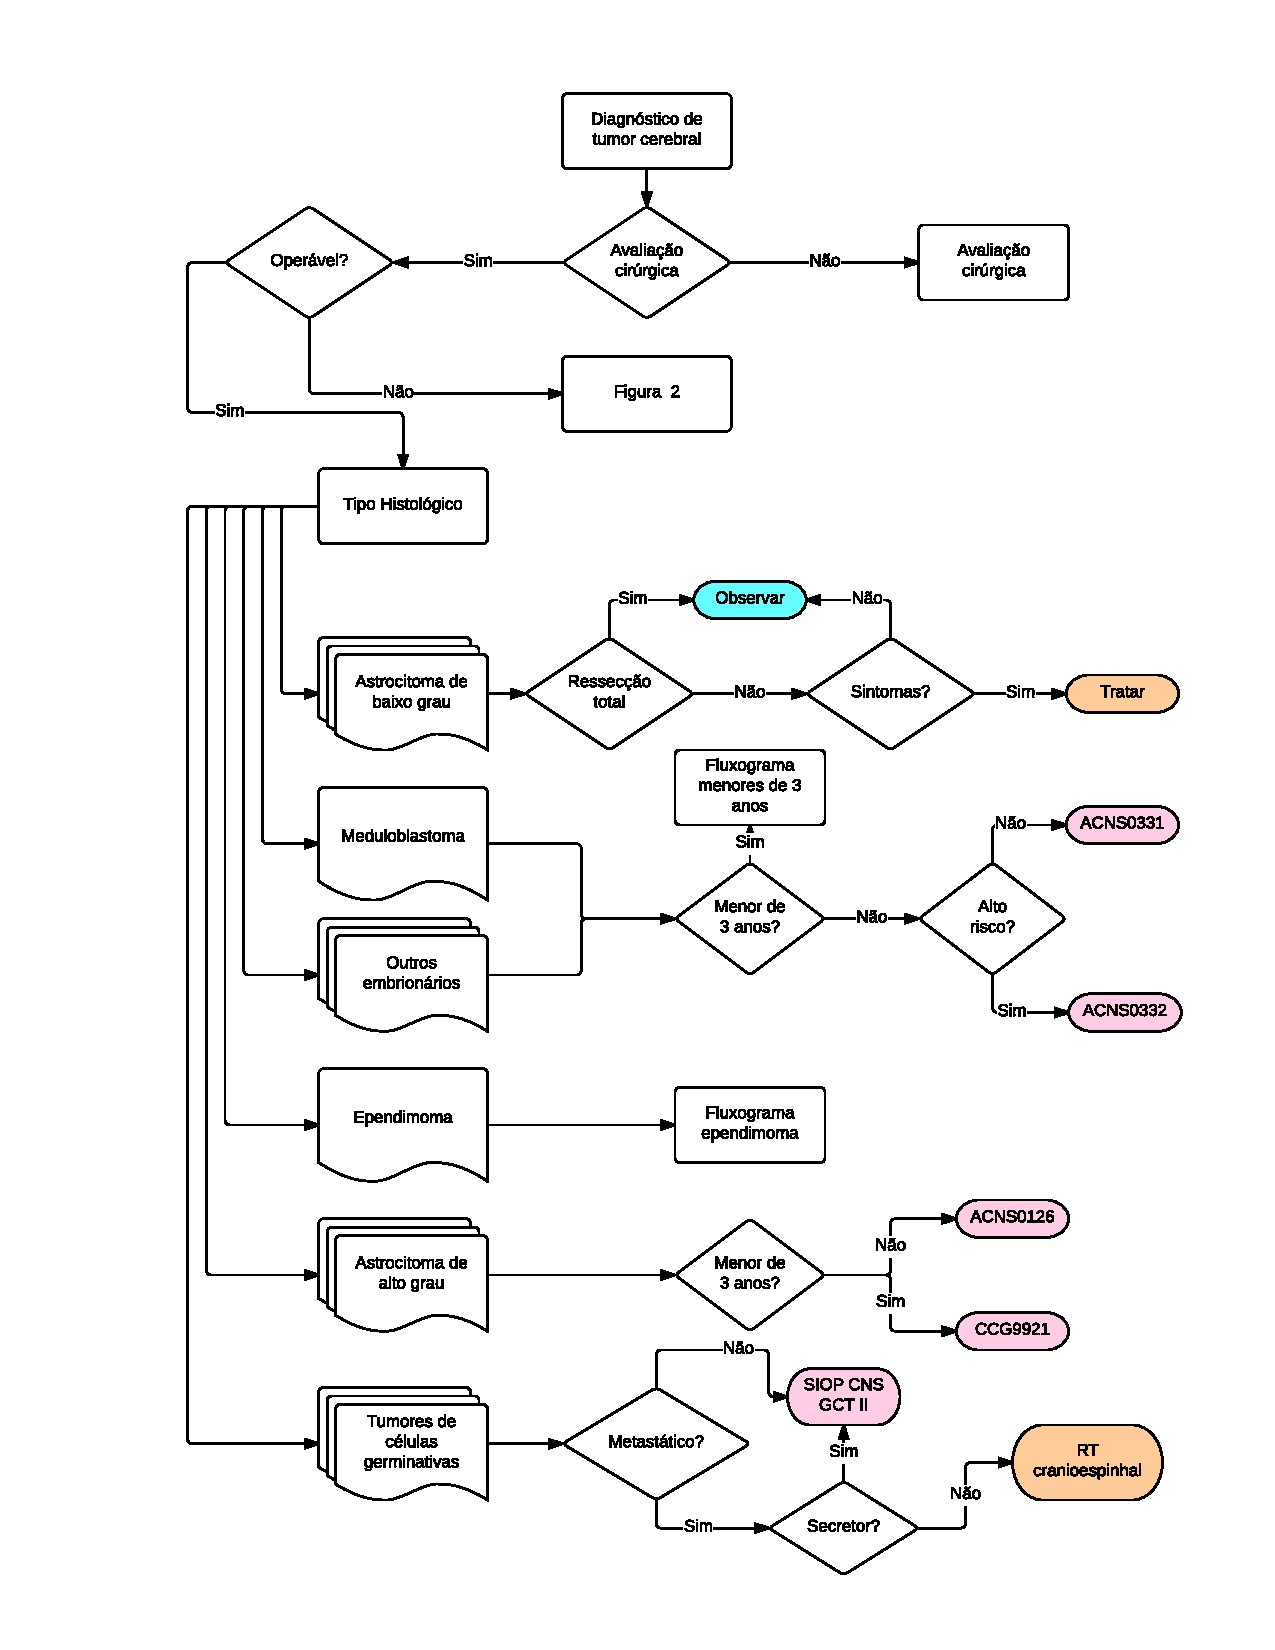
\includegraphics[scale=0.8,trim = 10mm 10mm 8mm 5mm,clip]{fig/fig1.pdf}
\caption{Tratamento de crianças com tumores cerebrais, com histologia}
%\label{Rotulo}
\end{figure}
\clearpage
\begin{figure}[!htb]
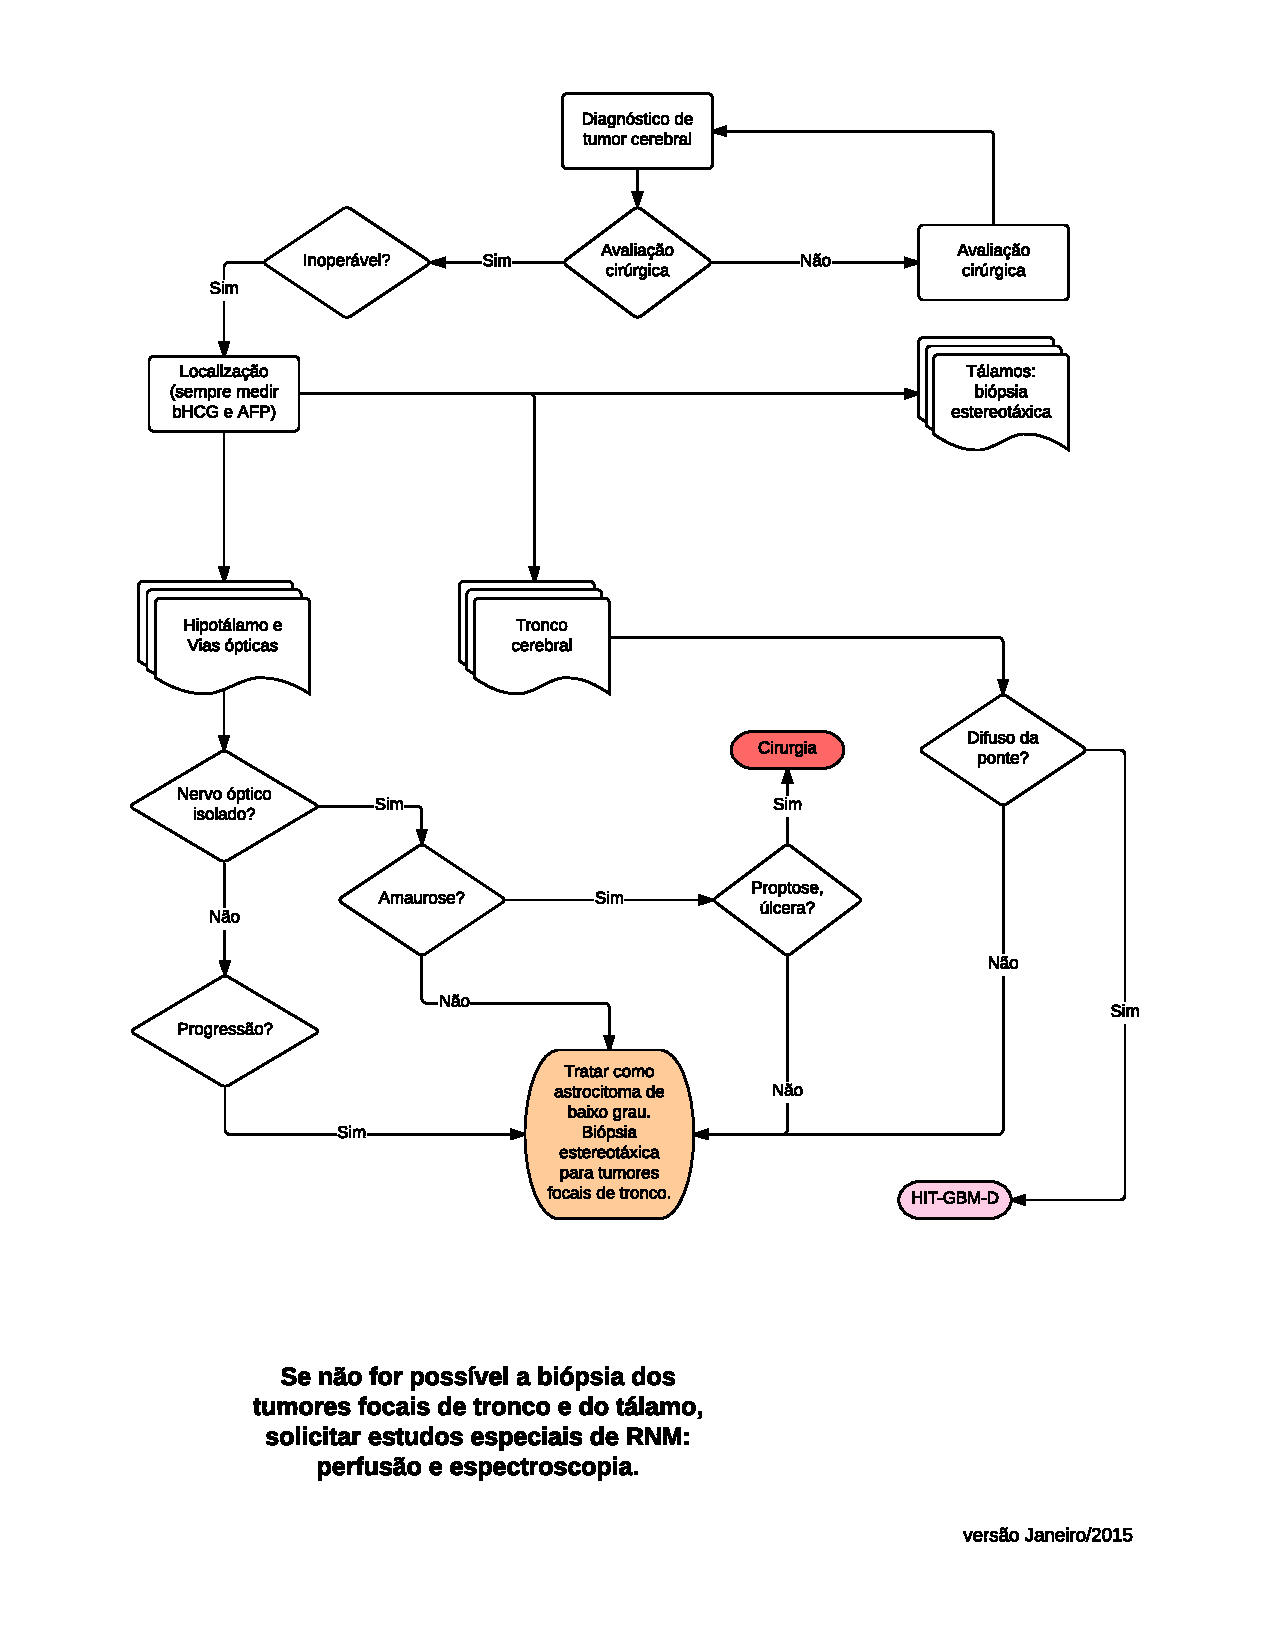
\includegraphics[scale=0.86,trim = 20mm 5mm 10mm 8mm,clip]{fig/fig2.pdf}
\caption{Tratamento de crianças com tumores cerebrais, sem histologia}
%\label{Rotulo}
\end{figure}
\end{center}

Os tumores cerebrais são um grupo heterogêneo de doenças neoplásicas de comportamento variável, com as características comuns de relativa raridade, elevada morbidade e elevada mortalidade. Dentre as neoplasias infantis, no entanto, constituem (como um grupo) o primeiro tumor sólido e a segunda neoplasia maligna mais frequente nas crianças, atrás apenas das leucemias, perfazendo em torno de \(20\%\) das neoplasias pediátricas. A sua incidência varia de acordo com a região do mundo. Nos EUA, a incidência anual ajustada para a idade de tumores cerebrais malignos primários na população de \(0-15\) anos foi de \(3,4\) por \(10^5\) pessoas-ano entre \(2004-2008\) \cite{Ostrom01102014}. Já na Europa, entre \(1988-1997\), a incidência reportada foi de \(2,99\) por \(10^5\) \cite{Peris-Bonet}. Esta incidência é mais alta do que a usualmente reportada na Ásia, onde relatos indicam entre \(1,8-2,2\) casos por \(10^5\) \cite{CNCR21430}. No Brasil, o primeiro relato do Registro de Câncer de Base Populacional indicou uma incidência de \(0,9\) a \(3,2\) por \(10^5\), semelhante à estatística do mundo desenvolvido ocidental \cite{IJC24799}. Fortaleza teve uma das menores incidências relatadas, \(1,3\) casos por \(10^5\), o que pode indicar subdiagnóstico. Hoje em dia, no entanto, já não é apropriado falar em “tumores cerebrais” infantis, sem separar as diversas entidades patológicas entre si, as quais têm incidência, tratamento e prognóstico muito díspares.

Os tumores cerebrais mais frequentes em crianças são os astrocitomas pilocíticos, tumores de comportamento incerto, ora classificados como benignos, ora como malignos. Eles representam em torno de 1\(8\%\) dos tumores cerebrais infantis. Em seguida, vem os tumores embrionários, a maior parte dos quais meduloblastomas, os tumores malignos mais comuns da infància, que representam em torno de \(15\%\) dos diagnósticos de tumor cerebral em crianças \cite{Ostrom01102014}. Astrocitomas pilocíticos são tumores indolentes, de crescimento lento, tratados principalmente pela ressecção cirúrgica, a qual é curativa na maioria dos casos, com pouca probabilidade de disseminação e virtualmente ausência de transformação maligna \cite{gan}. Já os meduloblastomas são tumores indiferenciados, com elevado índice mitótico, com acentuada propensão à disseminação e recidiva, necessitando de terapia adjuvante com radioquimioterapia após ressecção cirúrgica \cite{partap}. Estes dois tipos tumorais, que juntos correspondem a mais de \(30\%\) dos casos de tumores cerebrais em crianças, têm hoje um excelente prognóstico quando comparado ao passado. Outros tipos tumorais menos frequentes, todavia, têm resultados menos brilhantes com o tratamento atualmente disponível. Tumores de tronco cerebral, normalmente não biopsiados na sua maioria, constituem cerca de \(10\%\) dos tumores cerebrais infantis, e têm um prognóstico extremamente reservado, com apenas um subgrupo pequeno de pacientes com tumores neste sítio alcançando sobrevida prolongada.

O tratamento de tumores cerebrais em crianças e adolescentes evoluiu significantemente nas últimas décadas. Dos anos 80 até hoje, o conhecimento sobre o papel das várias modalidades de terapia (cirurgia, radioterapia e quimioterapia) ficou mais claro e programas terapêuticos específicos para cada tipo de doença puderam ser desenvolvidos. Hoje em dia, a maioria das crianças com um diagnóstico de tumor cerebral conseguirá ser adequadamente tratada e alcançará sobrevida prolongada. O manejo dos efeitos colaterais a longo prazo da terapia e das sequelas da doença são as principais preocupações na neuro-oncologia pediátrica moderna \cite{merchant}. No Brasil, estudos de sobrevida de pacientes pediátricos com tumores cerebrais são raros. Nosso grupo publicou recentemente uma análise de sobrevida de \(103\) pacientes pediátricos diagnosticados com tumores cerebrais entre 2000 e 2006 num único centro hospitalar, mostrando resultados que se assemelham aqueles dos registros populacionais dos EUA e Europa para as principais patologias \cite{araujo}.

\section{Qual o objetivo desta obra}

O Hospital Infantil Albert Sabin (HIAS) é uma instituição hospitalar da administração direta da saúde da Secretaria de Saúde do Estado do Ceará, habilitado como unidade de assistência de alta complexidade em neurologia/neurocirurgia, UNACON exclusiva de oncologia pediátrica, UTI pediátrica nível II e hospital de ensino, nível de atenção de alta complexidade, atendendo pelo SUS \cite{cnes}. O Centro Pediátrico do Câncer é o anexo do HIAS onde o tratamento oncológico clínico é realizado, contando ainda com equipe multiprofissional de atenção às crianças com câncer. Tem \(22\) leitos de internação em enfermaria (\(2\) isolamentos), \(06\) leitos de UTIP, e \(05\) consultórios para atendimento ambulatorial. O ambulatório e a enfermaria contam com material para atendimento às urgências e emergências, incluindo carrinho de emergência completo com drogas e equipamento para reanimação. O CPC conta com plantão médico 24h por dia.

O HIAS-CPC é referência estadual para o tratamento de crianças com tumores cerebrais, servindo uma população de 8,8 milhões de habitantes (um e meio milhão de crianças e jovens até 18 anos) \cite{estat}. A incidência ajustada para a idade de tumores cerebrais pediátricos no Ceará foi estimada em \(1,3\) casos por \(10^5\), entre 1998 e 2002 \cite{inca}. Seu papel é fundamental para o diagnóstico, tratamento e acompanhamento de centenas de crianças com câncer, incluindo tumores cerebrais. O HIAS-CPC recebeu cerca de \(35\) novos pacientes com tumores cerebrais ao ano entre 2007 e 2013 (um total de \(250\)). Isto indica que a esmagadora maioria das crianças com esta doença no estado do Ceará são tratadas no HIAS-CPC. Dessa forma, torna-se imprescindível que a qualidade da atenção à saúde dispensada a estes pequenos pacientes em nosso serviço hospitalar seja continuamente revisada, avaliada e padronizada.

\section{Como esta obra foi feita}

\subsection{Revisão da literatura}
Os autores utilizaram uma estratégia de busca de mapeamento (mapping review) a fim de estabeler o panorama do conhecimento atual sobre o tratamento de tumores cerebrais em crianças (revisão da literatura, revisão narrativa) \cite{grant,vosgerau}. Uma busca foi realizada no PubMed com os termos “low grade glioma”, “medulloblastoma”, “high-grade glioma”, “brainstem tumor”, “combined treatment” e os filtros “all children” e "clinical trial” (busca original: \texttt{http://bit.ly/fhcflx-2DIR}). O número total de entradas conseguidas com esta estratégia foi de 271 publicações. Uma atualização da busca foi realizada logo antes da publicação da última versão desta obra, com o acréscimo de mais 41 trabalhos \texttt{http://bit.ly/fhcflx-2pnA}. Foram excluídas aquelas sobre adultos ou outras patologias fora do interesse da revisão e também aqueles com mais de 2 décadas e incluídos preferencialmente os ensaios clínicos fase 1, 2 e 3 e as revisões sistemáticas. A bibliografia dos trabalhos selecionados foi checada para identificar trabalhos dentro do escopo do projeto. Os trabalhos incluídos no final são os citados na bibliografia da revisão, nesta obra. Os trabalhos foram revisados e qualificados segundo a nova classificação de níveis de evidência da OCEBM \cite{ocebm}. De acordo com a classificação 2011 da OCEBM, os ensaios controlados e randomizados são considerados evidência de nível 2, enquanto os estudos não controlados e séries de casos (equivalentes) são considerados evidência de nível 4 (tratamento). Nenhum trabalho com nível 3 de evidência (controlados, porém não randomizados) foi encontrado. Alguns ensaios foram desenhados para obter informações sobre história natural da doença. Grandes coortes para estudo de prognóstico (\textit{inception cohort}) são consideradas nível 2 de evidência, enquanto coortes de qualidade menor ou grupos controle de ensaios randomizados são nível 3.

A partir deste mapeamento, foram selecionados os tratamentos com maior qualidade de evidência. Lacunas no conhecimento atual foram listadas (não exaustivamente). Esta evidência foi usada para esboçar um plano ótimo de tratamento para os pacientes. As dúvidas em relação a indicação de modalidades específicas de tratamento foram discutidas e possíveis implementações práticas foram sugeridas. O resultado é um texto cujo objetivo é esclarecer quais as opções de tratamento disponíveis, quais são amplamente aceitas como padrão, onde existe controvérsia e onde a evidência está faltando para indicar um determinado tratamento. O intuito não é ser uma diretriz ou protocolo (vide definições), mas embasar a análise crítica dos protocolos utilizados no serviço do Hospital Infantil Albert Sabin (HIAS), para o tratamento de crianças e adolescentes portadores de tumores cerebrais.

\subsection{Protocolos de tratamento utilizados no HIAS}

Na segunda parte desta obra, os protocolos utilizados para tratar os pacientes com tumores do sistema nervoso central no HIAS foram listados e apresentados. Avaliamos todos os protocolos de tratamento utilizados no nosso serviço hospitalar para tratar crianças e adolescentes com tumores do sistema nervoso central, atraveés de revisão de prontuários. O período avaliado foi os últimos 16 anos. Um total de 262 pacientes foram tratados com quimioterapia antineoplásica citotóxica sistêmica nesse período. Destes, 105 (40\%) estavam vivos até a última atualização desta obra. Os protocolos de tratamento clínico usados em nosso serviço foram: COG-A9952 \cite{Ater20072012} (107 pacientes), SOBOPE 1998 (52 pacientes), HIT-GBM-C ou D \cite{Wolff2011} (22 pacientes), SLAOP 1993 \cite{slaop1} (21 pacientes), ACNS-0126 \cite{noq191} ou DUMC-1703 (16 pacientes), SIOP CNS GCT I ou II (14 pacientes), CCG-9961 \cite{4980} (10 pacientes), CCG-9921 \cite{095} (6 pacientes), COG-A99701 \cite{2792} (6 pacientes), outros (5 pacientes). 

Nos anexos desta obra, colocamos as fichas de tratamento que são usadas nos prontuários dos pacientes com tumores do sistema nervoso central tratados no HIAS. O tratamento apenas inicia depois que os pais ou responsáveis legais são informados sobre a proposta de tratamento e as opções disponíveis. Dividimos os anexos de acordo com o tipo de tratamento proposto para os pacientes: quimioterapia de primeira linha (protocolos usados via de regra como primeira escolha no tratamento, baseados na melhor evidência disponível modernamente), quimioterapia de resgate (usados para tratar doenças recorrentes, muitas vezes baseados em evidência mais limitada), quimioterapia neoadjuvante (realizada antes do tratamento cirúrgico definitivo) e quimioterapia metronômica (tem efeito anti-angiogênico e um esquema de doses pequenas e frequentes, em geral paliativo). Além disso, acrescentamos mais 3 seções para protocolos alternativos (substituídos por novos esquemas ou abandonados), terapia biológica, imunoterapia e terapia-alvo (usando anticorpos monoclonais, inibidores de tirosina quinase ou drogas imunomoduladoras), e protocolos experimentais (não usados na rotina de tratamento dos pacientes, apenas ensaios clínicos).

No capítulo sobre os protocolos usados no HIAS, forencemos maiores detalhes sobre como foram elaborados e como são usados no nosso serviço.

\chapter{O tratamento de tumores cerebrais em crianças}

\section{Tumores neuro-epiteliais de baixo grau}

\subsection{Avaliação crítica de ensaios clínicos}
\begin{figure}[!htb]
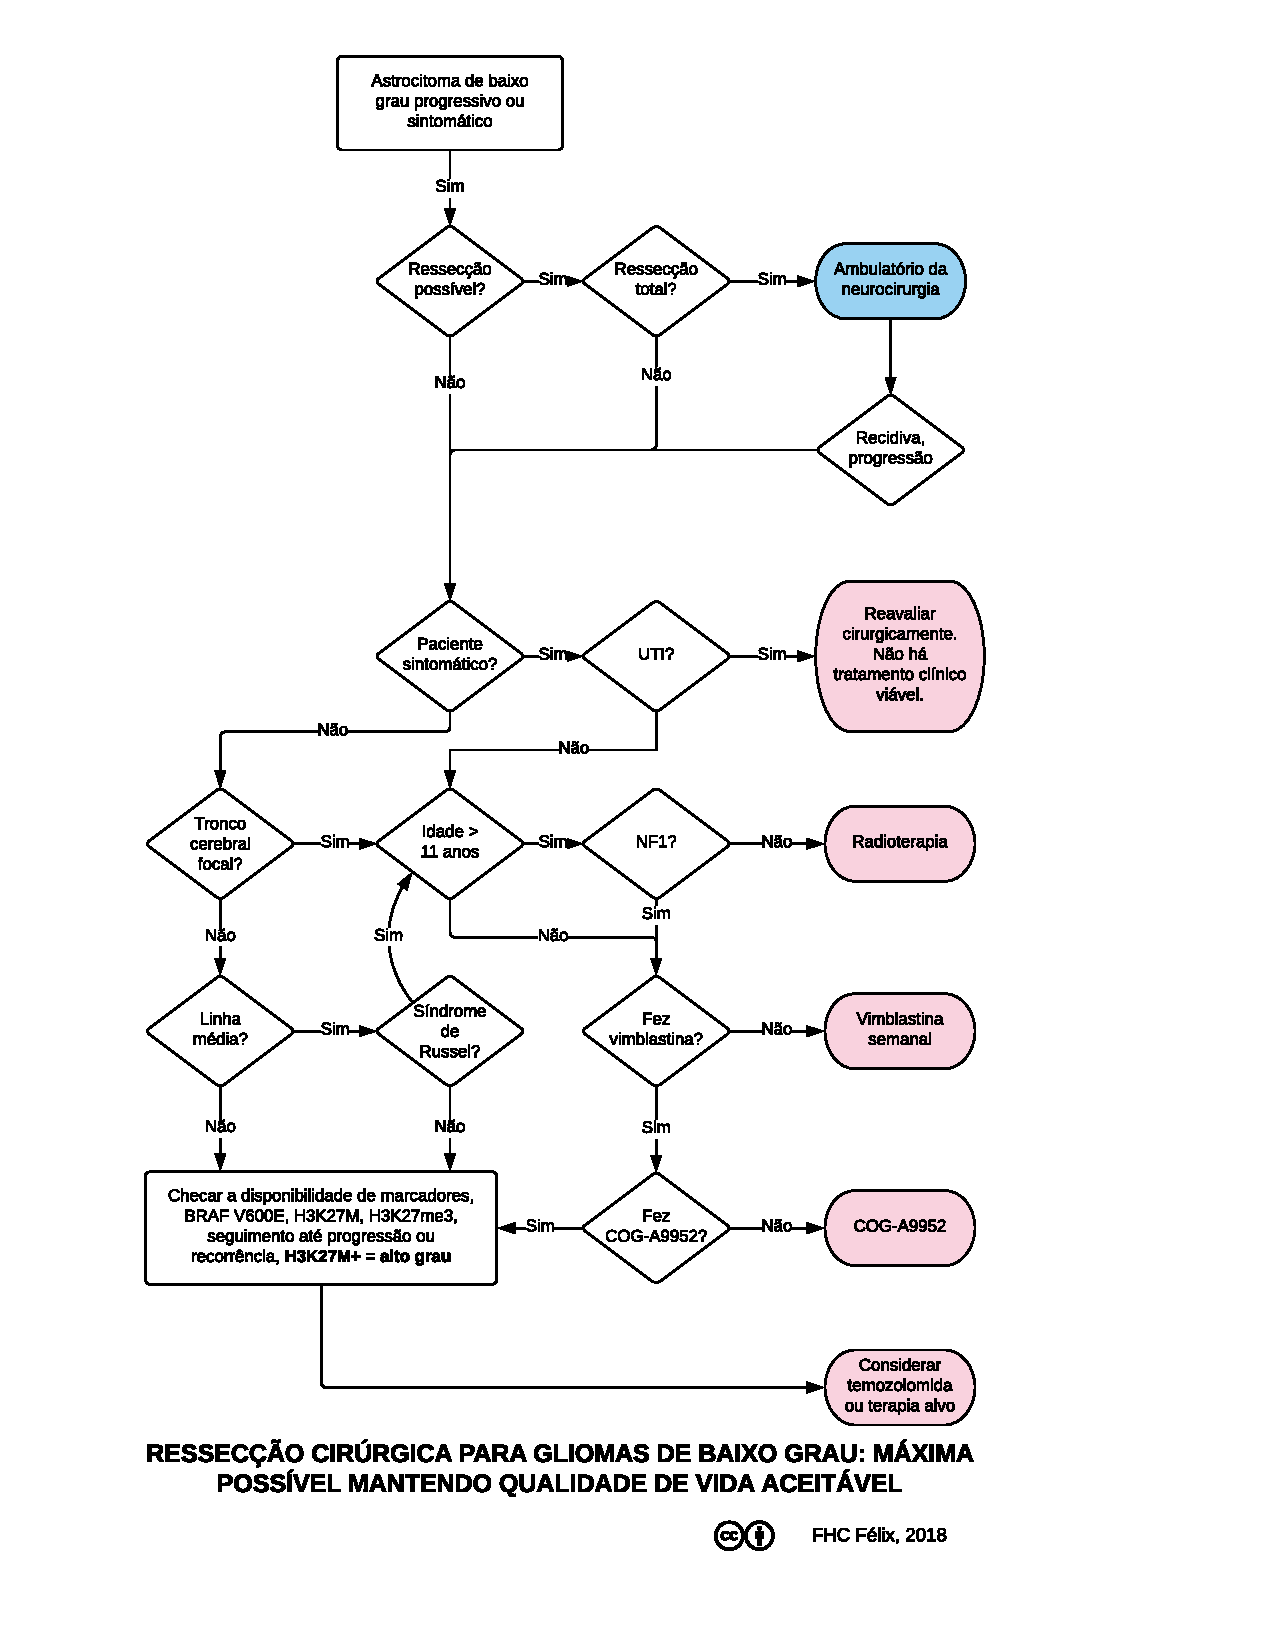
\includegraphics[scale=0.86,trim = 18mm 0mm 15mm 5mm,clip]{fig/fig3.pdf}
\caption{Tratamento de crianças com gliomas e outros tumores neuroepiteliais de baixo grau.}
%\label{Rotulo}
\end{figure}

Esse grupo inclui os astrocitomas, oligodendrogliomas, gangliogliomas e tumores neurogliais mistos ou variantes (grupos IIIa, b e d da CICI 3) \cite{CNCR20910}. A denominação de baixo grau refere-se à classificação da OMS para tumores do sistema nervoso central, a qual divide as neoplasias em 4 grupos, baseada em critérios histológicos. A classificação da OMS para tumores do sistema nervoso central constitui uma “escala de malignidade”, mais do que um esquema de estadiamento convencional \cite{louis}. Os tumores classificados como Grau I ou II são coletivamente denominados tumores de baixo grau de malignidade, enquanto aqueles classificados como Grau III ou IV são designados tumores de alto grau de malignidade. Os tumores de baixo grau são comumente tratados apenas cirurgicamente, com elevados índices de cura e sobrevida prolongada. Tumores astrocíticos e oligodendrogliais de baixo grau têm bom prognóstico associado à ressecção cirúrgica como única terapia. Todavia, a possibilidade de ressecção cirúrgica completa varia muito de acordo com o sítio tumoral \cite{wisof}.

Gliomas cerebelares são passíveis de ressecção completa em \(60-70\%\) dos casos, a maioria são astrocitomas pilocíticos (grau I) e seu comportamento é praticamente benigno \cite{gan}. A recidiva após ressecção e a progressão para tumores de maior grau de malignidade são muito raras. Mesmo tumores incompletamente ressecados mostram uma baixa propensão a progredir. A sobrevida livre de progressão em 5 anos após a cirurgia é de \(84-91\%\). A sobrevida livre de progressão em 5 anos em pacientes com doença residual é de \(54-63\%\) \cite{wisof}. 

Gliomas da via óptica e hipotálamo (e demais tumores diencefálicos ou da linha média) são lesões difusas, infiltrativas, em sua maioria astrocitomas de baixo grau (pilocítico ou difuso), com maior chance de disseminação e metástase no neuro-eixo, com maior incidência em pacientes com neurofibromatose tipo 1. Devido a sua natureza infiltrativa e ao risco de sequelas visuais e neuro-endócrinas, a ressecção cirúrgica não é realizada na maioria dos casos e a biópsia somente está indicada nos casos de imagem atípica. A maioria dos pacientes é tratada com base apenas em imagens sugestivas. Apesar de sua histologia, têm um prognóstico mais reservado do que os pacientes com lesões cerebelares \cite{gan}. A sobrevida livre de progressão em 5 anos é de \(47\%\) \cite{wisof}. 

Oligodendrogliomas, tumores mistos e variantes de tumores astrocíticos são raros em crianças (\(1\%\) ou menos de todos os tumores cerebrais). São tumores da substância branca supratentorial, infiltrativos, e o controle cirúrgico é curativo na maioria. Terapia adjuvante não está bem definida para estes tumores \cite{gan}. A sobrevida livre de progressão em 5 anos é de \(67\%\) \cite{wisof}.

O papel da cirurgia no controle dos gliomas de baixo grau está bem estabelecido. O estudo prospectivo multi-institucional do Children’s Oncology Group (COG) CCG9891 avaliou uma coorte de \(518\) pacientes diagnosticados com tumores de origem glial, tratados inicialmente com ressecção cirúrgica. Ocorreu revisão central da histologia de todos os casos incluídos. Do total, \(64\%\) dos pacientes não tinha evidência de doença residual após a cirurgia, \(20\%\) tinha doença residual limitada (\(< 1,5 cm^3\)) e \(16\%\) tinha doença residual significante (\(> 1,5 cm^3\)). A maioria dos pacientes (\(76\%\)) tinha astrocitoma pilocítico, \(6\%\) astrocitoma difuso, \(8\%\) ganglioglioma e \(10\%\) oligodendroglioma, tumores mistos ou variantes. A maioria dos pacientes (\(73\%\)) tinha 5 anos ou mais. A maioria (\(57\%\)) tinha tumores cerebelares, \(24\%\) de hemisférios cerebrais, \(14\%\) da linha média e \(4\%\) das vias ópticas ou hipotálamo. 

A sobrevida livre de progressão (SLP) em 5 anos de toda a coorte foi de \(80\%\), sendo \(84 \:a\: 91\%\) para tumores cerebelares, \(78\%\) para hemisférios cerebrais, \(65\%\) para a linha média e \(47\%\) para vias ópticas ou hipotálamo (\(p<0,001\)) (nível 2). A SLP em 5 anos foi de \(83\%\) para astrocitomas pilocíticos, \(88\%\) para gangliogliomas, \(66\%\) para astrocitomas difusos e \(67\%\) para outros tumores (\(p=0,64\)) (nível 2). Finalmente, a ressecção cirúrgica completa foi o fator isolado de maior impacto na progressão nesta coorte, \(94\%\) dos pacientes com ressecção completa estavam livres de progressão após 5 anos, enquanto \(59\%\) dos pacientes com doença residual limitada e \(53\%\) dos pacientes com doença residual significante alcançaram sobrevida livre de progressão prolongada (\(p<0,01\)) (nível 2). 

A conclusão é de que a ressecção completa deve ser tentada sempre que possível (ou seja, desde que não acarrete comprometimento funcional) para os pacientes pediátricos com gliomas de baixo grau (nível 4). Além disso, o fato de que mais de \(50\%\) dos pacientes com doença residual não progrediram em 5 anos indica que as intervenções terapêuticas adjuvantes devem ser postergadas até que ocorra progressão objetiva da doença. No entanto, apesar de sua histologia aparentemente benigna, \(44\%\) dos pacientes progrediram mesmo com doença residual muito limitada, o que indica a necessidade de monitorização dos pacientes com ressecção incompleta, independente da quantidade de tumor residual (nível 2) \cite{wisof}.

Fica evidente que um número significativo de pacientes pediátricos com gliomas de baixo grau sofre recidiva após controle cirúrgico ou não pode ter seu tumor ressecado. Nestes casos, indica-se terapia adjuvante com a intenção de evitar a progressão da doença. Vários estudos exploraram a contribuição da radioterapia e quimioterapia no tratamento de gliomas de baixo grau progressivos. 

Um ensaio fase II não controlado estudou \(78\) crianças com gliomas de baixo grau tratadas com radioterapia conformacional. Os pacientes tinham astrocitoma pilocítico (\(n=50\)), tumores de via óptica ou hipotálamo sem biópsia (\(n=13\)), astrocitoma difuso (\(n=4\)), ganglioglioma (\(n=3\)) e oligodendroglioma, tumores mistos ou variantes (\(n=8\)). A maioria dos tumores localizava-se no diencéfalo (\(47\)), \(17\) no cerebelo e \(3\) nos hemisférios cerebrais. Treze pacientes tinham NF-1, \(25\) receberam QT previamente e \(65\) sofreram cirurgia (biópsia ou ressecção incompleta). O tratamento foi indicado nos pacientes sintomáticos na avaliação inicial ou com evidência radiológica de progressão ou, ainda, com uma lesão residual numa área de risco para progressão. Dentre os pacientes cujo tratamento primário foi radioterapia, mais da metade iniciou o tratamento em menos de 90 dias após o diagnóstico. 

A SLP em 5 anos do grupo foi de \(87\%\). Treze pacientes apresentaram progressão com uma mediana de tempo de \(83\) meses. Quatro pacientes apresentaram falha terapêutica, desenvolvendo doença metastática. Não ocorreu diferença digna de nota entre os tipos histológicos (nível 2). Nenhum dos pacientes com NF-1 teve progressão ou malignização. Um paciente da série desenvolveu um glioma de alto grau na região do campo de irradiação, \(78\) meses após o tratamento. A incidência cumulativa de vasculopatia na série foi de cerca de \(5\%\) em 7 anos e o principal fator de risco para esta complicação foi a idade menor que 5 anos (nível 2) \cite{Merchant01082009}. Em relação aos efeitos cognitivos, um declínio de \(10\) pontos de QI foi estimado para crianças com 5 anos de idade ao tratamento, 5 anos após a radioterapia. O risco cumulativo de desenvolver insuficiência tireoidiana foi de \(64\%\) e de deficiência de GH foi de \(49\%\), em 10 anos. A incidência cumulativa de déficit auditivo foi de cerca de \(6\%\) em 10 anos. A presença de NF-1 foi um fator de risco para vasculopatia e déficit cognitivo (nível 2) \cite{Merchant01082009.2}. 

Em conclusão, esta série mostrou inequivocamente que a radioterapia pode controlar adequadamente os gliomas de baixo grau pediátricos não controlados cirurgicamente, com uma elevada proporção de pacientes tendo sobrevida prolongada sem progressão (nível 4). No entanto, isso ocorre às custas de frequentes efeitos colaterais, provavelmente permanentes. A radioterapia para gliomas de baixo grau deve ser evitada em pacientes com menos de 5 anos, devido ao risco de vasculopatia (nível 2). Apesar do risco cumulativo de déficit auditivo ser baixo e do fato do declínio cognitivo ser menor com o avançar da idade, adiar a radioterapia o quanto for possível parece razoável.

Com o intuito de atrasar o início da radioterapia, vários estudos foram realizados com diferentes esquemas de quimioterapia em crianças com gliomas de baixo grau recorrentes ou progressivos. As combinações mais utilizadas foram: carboplatina e vincristina \cite{packer,gnekow}; procarbazina, tioguanina, lomustina e vincristina (TPCV) \cite{prados}; cisplatina e etoposido \cite{mass}.

Packer \textit{et al} trataram \(78\) pacientes até 15 anos (idade média 3 anos, variando de 3 meses a 16 anos) com gliomas de baixo grau confirmados por histologia ou imagem típica, progressivos, reportando \(56\%\) de resposta radiológica objetiva e \(68 \pm 7\%\) de SLP em 3 anos (nível 4). A maioria dos pacientes (\(n=32\)) tinha astrocitoma fibrilar (difuso), \(17\) tinham astrocitoma pilocítico e \(26\) não tinham histologia. A maioria dos pacientes tinha tumores diencefálicos (\(n=58\)), \(12\) tinham no tronco e \(6\) em outros locais. Somente pacientes que sofreram ressecção de \(50\%\) ou menos das lesões foram admitidos. Não ocorreu revisão central de histologia ou imagens. Este ensaio clínico não avaliou se o esquema conseguia adiar o início da radioterapia, principal motivo do tratamento, devido ao curto tempo de seguimento \cite{packer}. 

A carboplatina fora testada pelo Pediatric Oncology Group (POG), em comparação com a iproplatina, num ensaio fase II, randomizado. Um grupo de pacientes pediátricos com tumores cerebrais histologicamente verificados, recorrentes ou progressivos, foi avaliado. O subgrupo de pacientes com astrocitoma de baixo grau (\(12\) pacientes, agregando pacientes de um ensaio não randomizado prévio do POG) não mostrou resposta radiológica objetiva, mas a maioria dos pacientes apresentou estabilização prolongada da doença com a carboplatina, o que motivou os pesquisadores a testá-la num grupo maior \cite{fried}. 

Prados \textit{et al}  trataram \(42\) crianças até 18 anos com gliomas de baixo grau histologicamente confirmados (exceto tumores de diencéfalo em pacientes com NF-1 ou de vias ópticas), com doença progressiva, utilizando a combinação TPCV. A SLP foi de \(45\%\) em 3 anos, com mediana de \(2,5\) anos para progressão (nível 4). A maioria dos pacientes tinha astrocitoma pilocítico (\(n=23\)), \(11\) tinham astrocitoma (sem outra especificação), \(6\) não tinham histologia e \(2\) tinham oligodendroglioma ou ganglioglioma. A maioria dos pacientes tinham tumores hipotalâmicos ou quiasmáticos (\(n=33\)), \(4\) talâmicos e \(5\) em outras localizações. A maioria dos pacientes sofreu ressecção parcial ou subtotal. Este esquema foi derivado de experimentos pré-clínicos que mostraram que a combinação das drogas utilizadas tinha efeitos sinérgicos nas células neoplásicas \cite{prados}. 

O ensaio não randomizado HIT-LGG 1996, do grupo de pediatria oncológica dos países de língua alemã (GPOH) utilizou um esquema de carboplatina e vincristina diferente daquele do COG. Um relato do subgrupo com gliomas hipotalâmico-quiasmáticos que recebeu quimioterapia (\(n=123\)) mostrou SLP de \(61\%\) em 5 anos \cite{gnekow} (nível 4). Os resultados completos do ensaio foram publicados em 2012 \cite{gnekow2}. Um total de \(1031\) pacientes foram recrutados, em um braço sem intervenção pós-cirurgia (ressecção total ou parcial, \(n = 668\)), e outro braço (não cirúrgico ou ressecção parcial) estratificado de acordo com a idade para receber vincristina-carboplatina (\(n = 216\)) ou radioterapia/braquiterapia convencional (\(n = 147\)). A idade média foi \(6,9\) anos, \(40\%\) dos pacientes tinha tumores de linha média e \(68\%\) tinha astrocitoma pilocítico. 

A sobrevida livre de eventos (SLE) em 5 e 10 anos relatada foi de \(47\%\) e \(44\%\) para o grupo tratado com quimioterapia e \(65\%\) e \(62\%\) para o grupo tratado com radioterapia. Entre os fatores afetando adversamente o prognóstico foram observados: ressecção cirúrgica imcompleta, idade < 1 ano ou > 11 anos, sítio tumoral de linha média (nível 4 para tratamento e nível 2 para prognóstico). Sessenta e um dos pacientes tratados com quimioterapia receberam radioterapia \(0,3-8,7\) anos após o primeiro tratamento. O ensaio não comparou o braço tratado apenas com cirurgia com aquele tratado com terapia adjuvante \cite{gnekow2}. 

Com o intuito de tentar melhorar estes resultados, a SIOP e o GPOH iniciaram conjuntamente o ensaio SIOP-LGG 2004, o qual terminou de cadastrar pacientes em 2012. Este ensaio randomizado comparou carboplatina e vincristina com carboplatina, vincristina e etoposido \cite{gnekow3}. Um total de \(497\) pacientes com glioma de baixo grau foram randomizados em dois grupos (\(249\) e \(248\)). A sobrevida livre de eventos em 5 anos foi de \(45-46\%\) e a sobrevida global em 5 anos foi de \(89\%\) em ambos os grupos. 

Concluiu-se que a adição de etoposido ao esquema de vincristina e carboplatina não mostrou nenhuma vantagem. Neste ensaio, a síndrome diencefálica e a idade ao diagnóstico foram fatores que afetaram adversamente o prognóstico. Os autores também questionaram o benefício real da quimioterapia para pacientes pediátricos com lesões do sistema óptico, pois neste ensaio não se demonstrou proteção da visão com a quimioterapia. A recidiva ou progressão nas primeiras \(24\) semanas correlacionou-se com elevada probabilidade de morte\cite{gnekow4}.

Em 2002, um grupo italiano relatou um grupo de 34 crianças com gliomas de baixo grau não ressecáveis, a maior parte hipotalâmico-quiasmáticos (\(n=29\)), tratadas com cisplatina e etoposide. Eles mostraram uma SLP de \(78\%\) em 3 anos, com \(11\) pacientes obtendo remissão parcial e 1 completa (nível 4). No entanto, uma quantidade significativa de pacientes apresentou toxicidade auditiva, um efeito colateral conhecido da cisplatina \cite{mass}.

Apesar da aparente superioridade da combinação carboplatina e vincristina, os ensaios tinham grandes diferenças entre si quanto aos diagnósticos histológicos e topográficos dos pacientes, além de diferenças na terapia prévia. Para definir qual o melhor dentre os dois esquemas, um ensaio fase III randomizado foi levado a cabo pelo COG e seus resultados publicados recentemente \cite{Ater20072012}. O estudo avaliou \(274\) pacientes com 10 anos ou menos, com gliomas de baixo grau e com doença residual (mais de \(5\%\) da lesão inicial ou \(1,5 cm^2\)) ou progressiva. Ocorreu revisão central das imagens e da patologia. Pacientes com tumores hipotalâmico-quiasmáticos foram incluídos com base nas imagens. 

A SLP em 5 anos foi de \(45\%\) para todo o grupo, sendo de \(39\%\) para o esquema carboplatina-vincristina e \(52\%\) para o esquema TPCV. Esta diferença não foi significante num teste de log-rank, mas mostrou-se significante num modelo de sobrevida com fração de cura (cure rate model), onde parte desta diferença deveu-se a pacientes com sobrevida prolongada (\(p<0,05\)) (nível 2). O ensaio encontrou dois preditores independentes da SLP: idade (menor risco entre 1 e 5 anos) e doença residual (menor risco se \(<3 cm^2\)) (nível 2).

Em 2016, o grupo de neuro-oncologia pediátrica do Canadá publicou os resultados de um ensaio fase II que testou a monoterapia com vimblastina semanal para pacientes pediátricos com tumores neuroepiteliais de baixo grau progressivos \cite{lassaletta}. Cinquenta e quatro pacientes (idade média 8 anos, variando de 0,7 a 17), a maioria (\(~ 50\%\)) com tumores da linha média anterior (quiasma óptico e hipotálamo) e astrocitoma pilocítico foram tratados com vimblastina semanal. Quarenta e sete pacientes (\(87\%\)) obtiveram pelo menos estabilização da doença. A SLP em 5 anos foi de \(53\%\) (intervalo ce confiança 95\% 41-68). Pacientes com NF-1 (17 pacientes) mostraram melhor sobrevida livre de progressão, \(85\% (IC95 68-100)\), do que pacientes sem NF-1 (\(42\%, IC95 29-60, p = 0.01\)). Não ocorreu diferença em relação à presença de alterações genéticas de BRAF (nível 4).

O resultado destes ensaios deve ser encarado com senso crítico. Apesar de todos os regimes terapêuticos aparentemente terem conseguido adiar a progressão nos pacientes estudados, nenhum estudo comparou os resultados com um grupo controle randomizado ou não. O fato de que o subgrupo com doença residual do ensaio CCG9891 também ter apresentado SLP equivalente indica que se deve ter cautela na indicação de tratamentos adjuvantes. Uma comparação entre os regimes e com um grupo controle não tratado parece estar justificada. Além disso, uma melhor caracterização dos subgrupos onde o tratamento farmacológico tem utilidade é necessário.

\subsection{O panorama molecular dos gliomas de baixo grau}

Até 2016, a classificação dos tumores do sistema nervoso central agregava o conhecimento anátomo-patológico e clínico acumulado em 130 anos de neuropatologia desde o trabalho pioneiro de Santiago de Ramón y Cajal \cite{pinero2014santiago}. Neste ano, a Organização Mundial da Saúde (OMS) publicou a revisão de sua quarta edição da Classificação dos Tumores do Sistema Nervoso Central \cite{Louis2016}. Pela primeira vez, a classificação incluiu dados moleculares oriundos de estudos genômicos empreendidos nos últimos 15 anos, desde a conclusão do Projeto Genoma Humano. Dessa forma, o conhecimento sobre as alterações moleculares mais frequentes em gliomas de baixo grau foram agregadas à avaliação clínico-patológica destes tumores, com valor prognóstico já demonstrado. Este novo conhecimento ainda não originou mudanças na prática clínica, tanto em termos de estratificação de grupos de risco, quanto em relação à terapia. No entanto, isso será somente questão de tempo. Até o momento, acumulam-se relatos de casos publicados mostrando resposta de pacientes com gliomas de baixo grau com alterações moleculares bem definidas à terapia alvo direcionada a estas alterações moleculares. Desa forma, é provável que os ensaios clínicos do futuro passem a estratificar os pacientes de acordo com a classificação molecular e que eles sejam tratados de acordo com medicações sem citotoxidade geral, como os inibidores de tirosina quinase \cite{now209}.

A principal doença desse grupo a ter seu panorama molecular definido também é a mais comum em crianças e adolescentes: astrocitoma piloćitico. Em 2008, foi descrita uma duplicação gênica em tandem no locus 7q34, a qual criava um gene quimérico pela fusão KIAA1549:BRAF em 29 de 44 casos de pacientes com astrocitoma pilocítico. O produto gênico é uma proteína com atividade proteína quinase constitutiva capaz de transformar células gliais \cite{Jones8673}. Essa foi a primeira mutação deste tipo (rearranjo gênico) afetando a via RAS/RAF documentada em um tumor esporádico. Uma avaliação de 64 casos pediátricos de astrocitoma pilocítico mostrou a presença da mutação pontual V600E do gene BRAF em 6 pacientes e uma mutação B-Raf\textsuperscript{insT}(inserção causando duplicação da treonina 599) em mais 2 pacientes\cite{IJC25893}. Somando-se o número de pacientes com astrocitoma pilocítico que comumente têm NF-1 ou fusões mais raras com RAF1, pode-se concluir que cerca de 80-90\% dos pacientes com esse tumor apresentam uma mutação da via MAPK/ERK (\textit{mitogen-activated protein kinase/extracellular signal-regulated kinase}, caracterizando esta via de sinalização celular como crítica para a gênese deste tumor \cite{Jones2012}. Aparentemente, as diversas mutações são mutuamente excludentes no astrocitoma pilocítico, ou seja os pacientes negativos para a fusão KIAA1549:BRAF ou têm o gene não mutado ou BRAF\textsuperscript{V600E} (ou ainda uma outra mutação mais rara de BRAF). O perfil molecular também influencia a localização dos tumores: NF1 e mutações pontuais de BRAF são mais comuns em tumores de linha média, já as fusões envolvendo BRAF ou RAF1 são mais encontradas no cerebelo \cite{Jones2012}. 

A fusão KIAA1549:BRAF nunca foi demonstrada de forma incontroversa em outros gliomas que não o astrocitoma pilocítico, o que parece indicar que é uma alteração genética praticamente exclusiva deste tumor. Isso dá valor diagnóstico importante em casos de dúvida. De fato, a tendência é considerar os raros casos de "outros gliomas" positivos para esta fusão como sendo, na verdade, variantes histológicas incomuns do astrocitoma pilocítico \cite{Jones2012}. Em contraste, a mutação BRAF\textsuperscript{V600E} não é exclusiva de um tipo tumoral apenas, ocorrendo em mairo frequência em casos de melanoma, carcinoma de cólon e de tireóide. Além de uma pequena porcentagem de astrocitomas pilocíticos, essa mutação é encontrada em vários gliomas de baixo grau menos comuns. Uma análise de \(1320\) casos de tumores primários do sistema nervoso central mostrou positividade de BRAF\textsuperscript{V600E} em \(42\) de \(64\) (\(66\%\)) de xantoastrocitomas pleomórficos, 15 de 23 (65\%) de xantoastrocitomas pleomórficos anaplásicos, \(14\) de \(77\) (\(18\%\)) de gangliogliomas e \(9\) de \(97\) (\(9\%\)) de astrocitomas pilocíticos. Neste último tumor, um terço foram detectados em tumores diencefálicos \cite{Schindler2011}. Dessa forma, a via MAPK/ERK de sinalização celular surge como a principal envolvida na gênese dos gliomas de baixo grau de uma forma em geral, especialmente astrocitoma pilocítico, ganglioglioma e xantoastrocitoma pleomórfico.

Outras alterações genéticas têm sido descritas neste grupo de tumores, sendo que uma das mais recentes é a presença de mutações dos genes MYB e MYBL1 no glioma angiocêntrico e astrocitoma difuso \cite{Tatevossian2010}. Uma avaliação genômica de \(91\) tumores neuroepiteliais de baixo grau menos comuns identificou um marcador genético único em \(84\%\) dos casos. Uma fusão MYB-QKI foi identificada em \(87\%\) dos gliomas angiocêntricos e rearranjos envolvendo MYB/MYBL1 foram encontradas em \(41\%\) dos astrocitomas difusos. Esses dados comprovam alterações destes genes como as mais importantes nestes dois tipos de tumores gliais \cite{Qaddoumi2016}. Mutações pontuais de FGFR1 são as mais comuns em gliomas de baixo grau depois da mutação BRAF\textsuperscript{V600E} \cite{now209}. Uma alteração genética de FGFR1, incluindo mutações pontuais, duplicações internas do domínio quinase e fusões foram encontradas em \(82\%\) de DNET (\textit{dysembrioplastic neuroepithelial tumors}) e \(40\%\) de tumores oligodendrogliais, na mesma avaliação genômica.

Fica claro pelos dados de pesquisa genômica associada com clínica nos últimos \(10-15\) anos que as alterações moleculares mais frequentes em tumores neuroepiteliais de baixo grau ocorrem em 3 genes: BRAF, MYB e FGFR1 \cite{now209,Qaddoumi2016}. Outras alterações moleculares descritas parecem girar em torno das vias de sinalização molecular representadas por estes mesmos genes. Isso abre uma nova era de possibilidades para diagnóstico e terapia baseadas em biologia molecular. Os ensaios clínicos do futuro vão rapidamente agregar estes dados para definir subgrupos de prognóstico bem definido e validar o tratamento com terapia-alvo.

\subsection{Questões importantes ainda por responder}

A evidência apresentada até o momento deixa uma série de lacunas em nosso conhecimento sobre o tratamento clínico de tumores neuroepiteliais de baixo grau em crianças e adolescentes. Entre as diversas questões que podemos levantar, algumas podem ser apontadas como mais evidentes:

\begin{enumerate}
\item Pacientes com tumor residual maior que \(1,5 cm^2\) e menor que \(3,0 cm^2\) serão melhor seguidos com conduta expectante? 
\item Para pacientes com mais de 5 anos e mais de \(3,0 cm^2\) de tumor residual, deve-se indicar radioterapia precocemente? 
\item A quimioterapia tem papel restrito aos pacientes menores de 5 anos com progressão documentada e naqueles com gliomas hipotalâmico-quiasmáticos? 
\item Deve-se adaptar a estratégia terapêutica de acordo com o sítio tumoral?
\item A vimblastina semanal deve ser a primeira escolha de tratamento quimioterápico?
\item Qual o melhor tratamento após falha terapêutica múltipla (progressão após dois tratamentos com quimioterapia e/ou radioterapia)?
\end{enumerate}

A ausência de ensaios comparativos entre as abordagens terapêuticas e de ensaios com controles não tratados impede a resposta destas questões com certeza. A realização de ensaios clínicos com desenho e poder estatístico para responder estas questões com a maior certeza possível vai exigir uma inédita colaboração internacional, com a participação ativa de centros de tratamento ao redor do mundo. A partir desse esforço, será possível oferecer o melhor e mais eficiente tratamento a todas as crianças e adolescentes com esta patologia.

\subsection{Conclusões}

A conclusão sobre a terapia dos tumores neuroepiteliais de baixo grau é de que, hoje em dia, temos evidência de relativa boa qualidade documentando a história natural deste grupo de tumores, mas a ausência de adequados estudos controlados e randomizados ainda suscita dúvidas quanto à melhor conduta em cada situação. A partir dos dados que temos até o momento, um esquema racional de tratamento para gliomas de baixo grau pediátricos inclui:

\renewcommand{\labelenumi}{\Alph{enumi}}
\begin{enumerate}
\item - A melhor ressecção cirúrgica possível (mantendo ao máximo a função) (nível 2)
\item - Seguimento de todos os pacientes com doença residual (independente da quantidade) (nível 2)
\item - Aguardar a progressão (ou piora sintomática) para indicar terapia adjuvante (mesmo quando doença residual) (nível 2)
\item - Evitar radioterapia em menores de 5 anos e portadores de NF-1 através do uso de quimioterapia (TPCV um pouco superior a carboplatina-vincristina, vimblastina parece ser equivalente) (nível 4)
\item - Tratar com radioterapia lesões progressivas após cirurgia e/ou quimioterapia, em maiores de 8-10 anos (nível 4)
\end{enumerate}

Infelizmente, mesmo com essa abordagem baseada em evidência, uma quantidade significativa de pacientes terá doença progressiva apesar da melhor terapia, mostrando que o tratamento ótimo dos tumores neuro-epiteliais de baixo grau pediátricos ainda não foi atingido. A incorporação de marcadores moleculares e melhor definição de subgrupos de risco devem ser prioridades na agenda da pesquisa clínica.

\section{Tumores embrionários e pineoblastoma}

\begin{figure}[!htb]
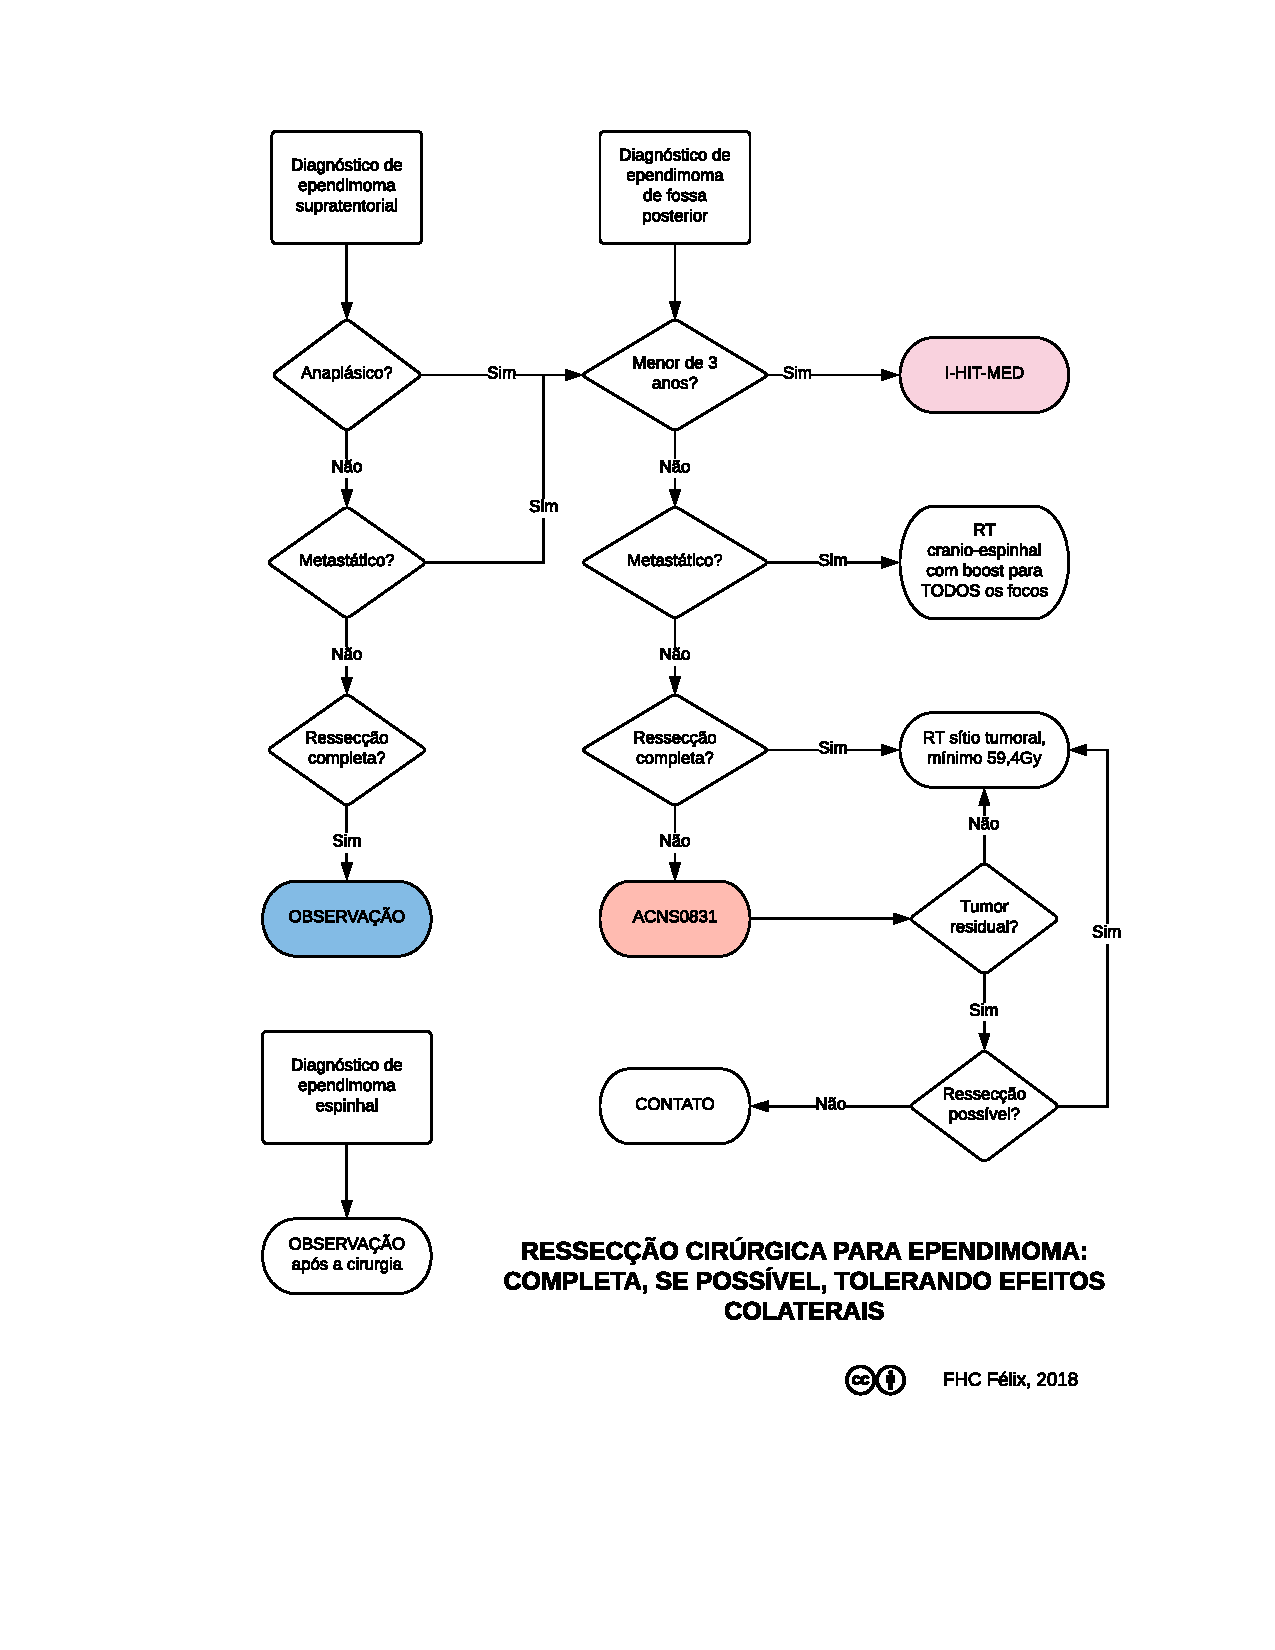
\includegraphics[scale=0.87,trim = 18mm 30mm 15mm 12mm,clip]{fig/fig4.pdf}
\caption{Tratamento de crianças com ependimomas.}
\end{figure}


\begin{figure}[!htb]
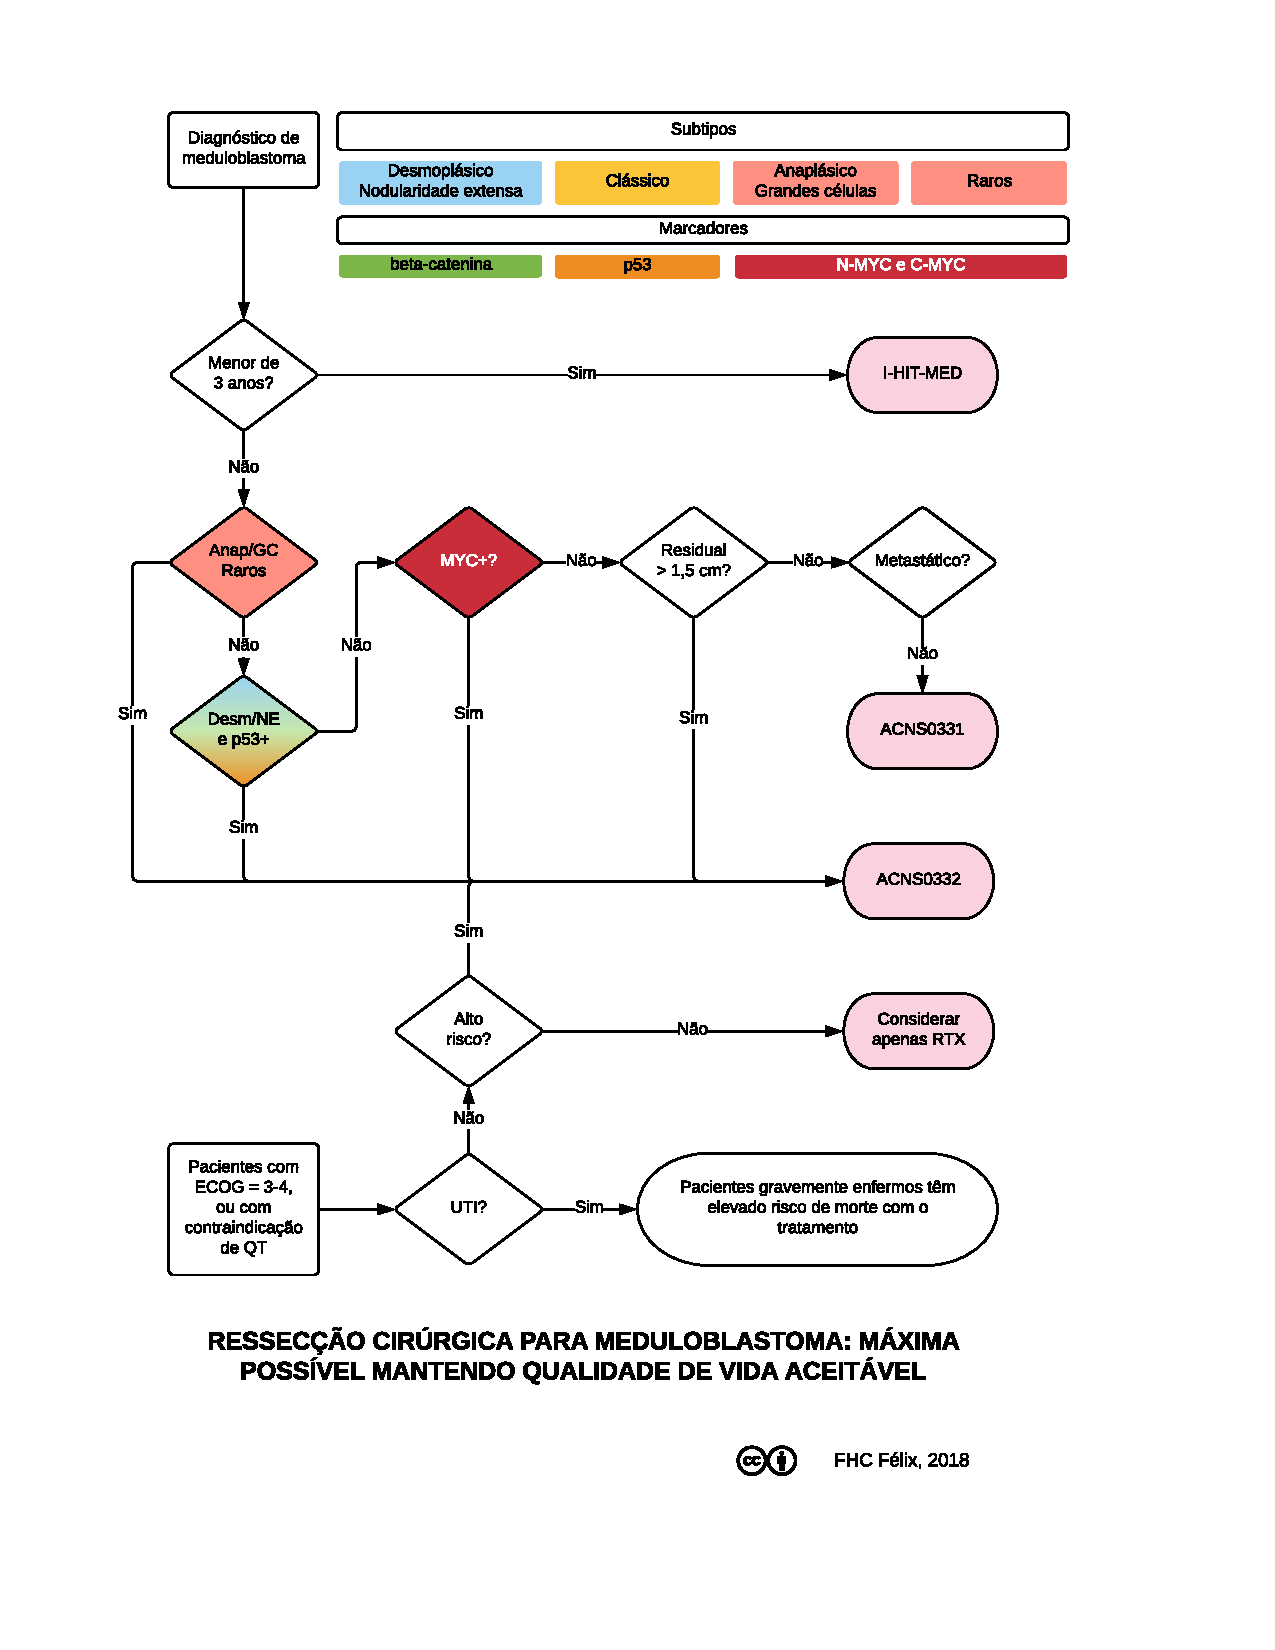
\includegraphics[scale=0.87,trim = 18mm 28mm 15mm 12mm,clip]{fig/fig5.pdf}
\caption{Tratamento de crianças com meduloblastomas.}
\end{figure}

Tumores embrionários incluem o meduloblastoma (mais comum deste grupo e o tumor cerebral maligno mais frequente em crianças e adolescentes), tumor teratóide-rabdóide atípico, tumor embrionário formador de rosetas em multicamadas, tumor embrionário sem outra especificação (SOE) e outros tumores mais raros. 

\begin{center}
\begin{table}
\renewcommand{\arraystretch}{1.5}
	\caption{\tiny }
\begin{tabular}{c|c|c|c|c|c}
	\hline
	\multicolumn{1}{c|}{\multirow{4}{*}{DMB}}&{0-5}&{M0}&{R0+}&{MYC/N(-/+)}&{P1}	\\
	\cline{2-6}
	\multicolumn{1}{c|}{}&\multicolumn{1}{c|}{\multirow{3}{*}{>5}}&{M0}&{R0}&{MYC/N(-/?)}&{P2}
	\\
	\cline{3-6}
	\multicolumn{1}{c|}{}&\multicolumn{1}{c|}{}&{M0/1}&{R+}&{MYC/N(+)}&{P3}
	\\
	\cline{3-6}
	\multicolumn{1}{c|}{}&\multicolumn{1}{c|}{}&{M2/3}&{R+}&{MYC/N(-/+)}&{P4}
	\\
        \hline
	\multicolumn{1}{c|}{\multirow{4}{*}{CMB}}&{0-3}&{M0}&{R0+}&{MYC/N(-/+)}&{P1}	\\
	\cline{2-6}
	\multicolumn{1}{c|}{}&\multicolumn{1}{c|}{\multirow{3}{*}{>4}}&{M0}&{R0}&{MYC/N(-/?)}&{P2}
	\\
	\cline{3-6}
	\multicolumn{1}{c|}{}&\multicolumn{1}{c|}{}&{M0/1}&{R+}&{MYC/N(+)}&{P3}
	\\
	\cline{3-6}
	\multicolumn{1}{c|}{}&\multicolumn{1}{c|}{}&{M2/3}&{R+}&{MYC/N(-/+)}&{P4}
	\\
        \hline
	\multicolumn{1}{c|}{\multirow{3}{*}{LCAMB}}&{0-3}&{M0}&{R0+}&{MYC/N(-/+)}&{P1}	\\
	\cline{2-6}
	\multicolumn{1}{c|}{}&\multicolumn{1}{c|}{\multirow{2}{*}{>4}}&{M0/1}&{R0+}&{MYC/N(-/+)}&{P3}
	\\
	\cline{3-6}
	\multicolumn{1}{c|}{}&\multicolumn{1}{c|}{}&{M2/3}&{R+}&{MYC/N(-/+)}&{P4}
	\\
	\hline
	\multicolumn{1}{c|}{\multirow{3}{*}{Pineoblastoma}}&{0-3}&{M0}&{R0+}&{MYC/N(-/+)}&{P1}	\\
	\cline{2-6}
	\multicolumn{1}{c|}{}&\multicolumn{1}{c|}{\multirow{2}{*}{>4}}&{M0}&{R0+}&{MYC/N(-/+)}&{P3}
	\\
	\cline{3-6}
	\multicolumn{1}{c|}{}&\multicolumn{1}{c|}{}&{M+}&{R+}&{MYC/N(-/+)}&{P4}
	\\
	\hline
	
\end{tabular}
\end{table}
\end{center}

\chapter{Esquemas de tratamento}

\section{Introdução}

No Centro Pediátrico do Câncer do Hospital Infantil Albert Sabin, utilizamos um total de 16 (dezesseis) protocolos de tratamento farmacológico para tumores cerebrais em crianças e adolescentes, baseados na literatura que foi citada neste manual. Estes protocolos foram adaptados a partir dos racionais dos ensaios clínicos descritos, com modificações pertinentes à realidade e disponibilidade de recursos em nosso serviço hospitalar. Além disso, quaisquer conclusões oriundas dos resultados destes ensaios clínicos, bem como informações de outros trabalhos e de outras fontes, foram usadas para adaptar os esquemas de tratamento à luz da melhor evidência disponível no momento em que este manual foi escrito. Alguns dos ensaios clínicos utilizados como modelo para parametrizar nossos protocolos ainda estão em andamento. Neste caso, apenas a parte não randomizada, não experimental dos esquemas foi adaptada e utilizada, mas não os braços de tratamento experimental ou não comprovado por evidências científicas.

\section{O que são estes protocolos}

Protocolo aqui significa um esquema de tratamento baseado em um ensaio clínico patrocinado por grandes grupos cooperativos de tratamento do câncer infantil. Nenhum destes protocolos inclui o texto completo ou trechos dos protocolos originais de pesquisa. Os pacientes tratados em nosso centro seguindo estes protocolos não estão sendo recrutados para pesquisa clínica. Estes protocolos também não constituem diretrizes terapêuticas, nem protocolos clínicos no sentido estrito, pois não foram elaborados por instituições ou grupos organizados, usando metodologia explícita. Nossos protocolos podem ser encarados como rotinas de manuseio dos pacientes e suas patologias, utilizados em nosso serviço hospitalar e baseados em evidências.

Pacientes com condições patológicas que não têm nenhum tratamento amplamente aceito, ou sobre as quais recaem controvérsias importantes quanto à terapêutica, são tratados com  protocolos baseados em evidências preliminares, como ensaios clínicos piloto ou fase I-II, ou ainda revisões de evidências observacionais. Não existem, no momento, ensaios clínicos experimentais abertos em nosso serviço. 

\section{Como utilizar estes protocolos}

Este manuscrito tem fins educativos e é voltado para falantes da língua portuguesa.  Embora este documento seja usado pelo responsável deste projeto como rotina de tratamento dos seus pacientes, o autor não pode responsabilizar-se pelo seu uso em outros locais e para o tratamento de outros pacientes, que não aqueles sob sua estrita supervisão. Os procedimentos e doses de medicamentos descritos no documento são no máximo possível fiéis ao empregado na literatura científica utilizada. No entanto, o autor não pode se responsabilizar por estas doses e seu uso, incluindo o manuseio não criterioso por profissional não habilitado para prescrever e administrar tais medicamentos. 

Apenas médicos registrados de acordo com a legislação vigente em seu país e devidamente habilitados por sociedades de cancerologia (hemato-oncologia) pediátrica devem usar este documento, em parte, ou no todo, e segundo seu juízo, para o tratamento de pacientes. Neste caso, o autor isenta-se de responsabilidade legal sobre quaisquer resultados, incluindo complicações, eventos adversos, prejuízos ou custos, advindos do uso deste documento, ou parte dele, por qualquer outro que não ele mesmo. Ao obter este documento a partir deste projeto, o usuário dele (o documento) está tacitamente concordando com estes e outros termos explicitados aqui.

\section{Declaração ética}

Este manuscrito não necessariamente representa os pontos de vista ou é endossado pelo Hospital Infantil Albert Sabin ou pela Secretaria de Saúde do Estado do Ceará, sendo de iniciativa do responsável pela sua elaboração.

Apesar de tratados conforme os racionais de ensaios clínicos conhecidos, os pacientes não estão sendo recrutados para pesquisa, e isso é deixado claro antes do início do tratamento. Quaisquer esquemas alternativos de tratamento aceitáveis do ponto de vista de chances de sucesso e risco de efeitos adversos são informados aos responsáveis pelos pacientes. Estes podem escolher livremente entre os protocolos propostos ou tratamentos alternativos aceitáveis.

\section{Formato e contribuições}

Nas páginas que se seguem, apresentamos as folhas de acompanhamento ambulatorial dos pacientes que estão em tratamento quimioterápico em nosso serviço hospitalar. Estas folhas são anexadas a cada prontuário do paciente e são preenchidas de acordo com o andamento do tratamento, anotando doses administradas, principais complicações, atrasos, modificações de doses, atualização de informações, entre outros dados. As versões aqui mostradas são as mais atuais quando da publicação deste manual.

O manual foi escrito em LaTeX, usando ShareLatex (depois Overleaf) e programas para desktop (Texmaker). Todo o código do projeto está disponível num repositório público do GitHub, que pode ser acessado neste endereço: \texttt{https://github.com/fhcflx/cpc-neuro.git}. O arquivo \texttt{*.tex} contém o código correspondente. Contribuições são bem-vindas. Se você ainda não tem uma conta no GitHub (gratuita), inscreva-se, abra uma pendência (\textit{issue}) ou faça uma cópia (\textit{fork}), modifique o que achar necessário e peça para integrar (\textit{pull request}) suas mudanças ao projeto. O sítio do projeto pode ser visitado neste endereço: \texttt{https://fhcflx.github.io/cpc-neuro}. 

\section{Uso não padronizado (\textit{off-label}) de medicamentos}

A definição da ANVISA (Agência Nacional de Vigilância Sanitária) para uso \textit{off-label} de medicamentos é a utilização de um medicamento aprovado para uma determinada indicação em um tratamento não previsto na bula (não aprovado). Isso inclui estudos \textit{a posteriori} que ampliam o uso de um medicamento para outras indicações e também o uso em outras doenças com base em similaridade fisiopatológica. Ainda de acordo com a ANVISA, o "uso \textit{off-label} é, por definição, não autorizado por uma agência reguladora, mas isso não implica que seja incorreto".

Na legislação brasileira atual, não existe regulamentação ou normatização sobre o uso não padronizado de medicamentos. O Conselho Federal de Medicina (CFM), em resposta a um processo-consulta, emitiu o parecer 2/16, no qual define que "os procedimentos médicos \textit{off label} são aqueles em que se utilizam materiais ou fármacos fora das indicações em bula ou protocolos, e sua indicação e prescrição são de responsabilidade do médico. Não compete às Comissões de Ética emitir juízo de valor sobre o uso de \textit{off label}." \cite{cfm}

Para o CFM, o papel das Comissões de Ética Médica e Comitê de Ética em Pesquisa deve ser educativo, uma vez que a responsabilidade do uso não padronizado é toda do médico prescritor. Assim, não há obrigação de reportar o uso não padronizado de medicamentos a nennuma instituição, da mesma forma que não existe exigência de consentimento informado por escrito no território nacional brasileiro para esse uso.

A utilização não padronizada de medicamentos é especialmente frequente na pediatria, uma vez que inexiste incentivo para que empresas que já tem produtos aprovados para adultos arquem com o dispendioso processo de registro da ampliação de seu uso para crianças. \cite{10.1001/archpedi.161.3.282} Uma avaliação mostrou mais de 80\% de prescrições \textit{off-label} em uma UTI neonatal. \cite{CARVALHO2012} Na oncologia pediátrica, existem poucas avaliações semelhantes, mas o uso não padronizado de medicamentos é potencialmente maior ainda. \cite{pmid21453298,10.1111/jcpt.12507}

No caso dos esquemas de tratamento aqui descritos, praticamente todas as medicações têm indicações não padronizadas, seja por faixa etária (etoposido, vincristina, carboplatina, etc) ou por indicação não prevista em bula (vimblastina, cisplatina, ifosfamida e outros). De todas as medicações citadas nesta obra, apenas a ciclofosfamida, a lomustina e a temozolomida (quando usada para tratar gliomas de alto grau) são utilizadas de acordo com a aprovação da ANVISA.

Diversos autores já frisaram a necessidade de mais estudos a fim de validar as indicações, apresentações e vias de administração próprias da pediatria de todas as drogas utilizadas na prática clínica. Uma iniciativa como essa não pode esperar a iniciativa privada, que têm baixa probabilidade de investir em um processo dispendioso e sem retorno financeiro. Seria papel dos governos regular e fomentar o desenvolvimento das aplicações pediátricas de drogas. Infelizmente, em nosso país não existe programa governamental que contemple esse problema.

\section{Avaliação de resposta:}

Não existem critérios de avaliação de resposta criados especificamente para serem utilizados na rotina clínica em pacientes pediátricos com tumores do sistema nervoso central. Os critérios de avaliação de resposta mais amplamente usados baseiam-se nos critérios de resposta da Organização Mundial da saúde (OMS)\cite{10.1093/jnci/92.3.205} e estão listados na tabela abaixo:

\begin{table}[h!]
	\begin{center}
		\begin{tabular}{l|c|c r}
			\multicolumn{2}{l}{\textbf{Resposta}} & \textbf{Método 2D} & \textbf{Método 3D}\\
			\hline
			Resposta completa & RC & Desaparecimento completo & Desaparecimento completo\\
			Resposta parcial & RP & Redução $\geq 50\%$ & Redução $\geq 65\%$ \\
			Resposta menor & RM & Redução $25-50\%$ & Redução $40-65\%$ \\
			Doença estável & DE & Mudança $< 25\%$ & Mudança $< 40\%$ \\
			Progressão & RP & Aumento $\geq 25\%$ & Redução $\geq 40\%$ \\
			\hline
			\multicolumn{4}{l}{\small{2D = bidimensional, 3D = tridimensional}}
		\end{tabular}
	\end{center}
\end{table}

\begin{figure}[h!]
	\begin{center}
		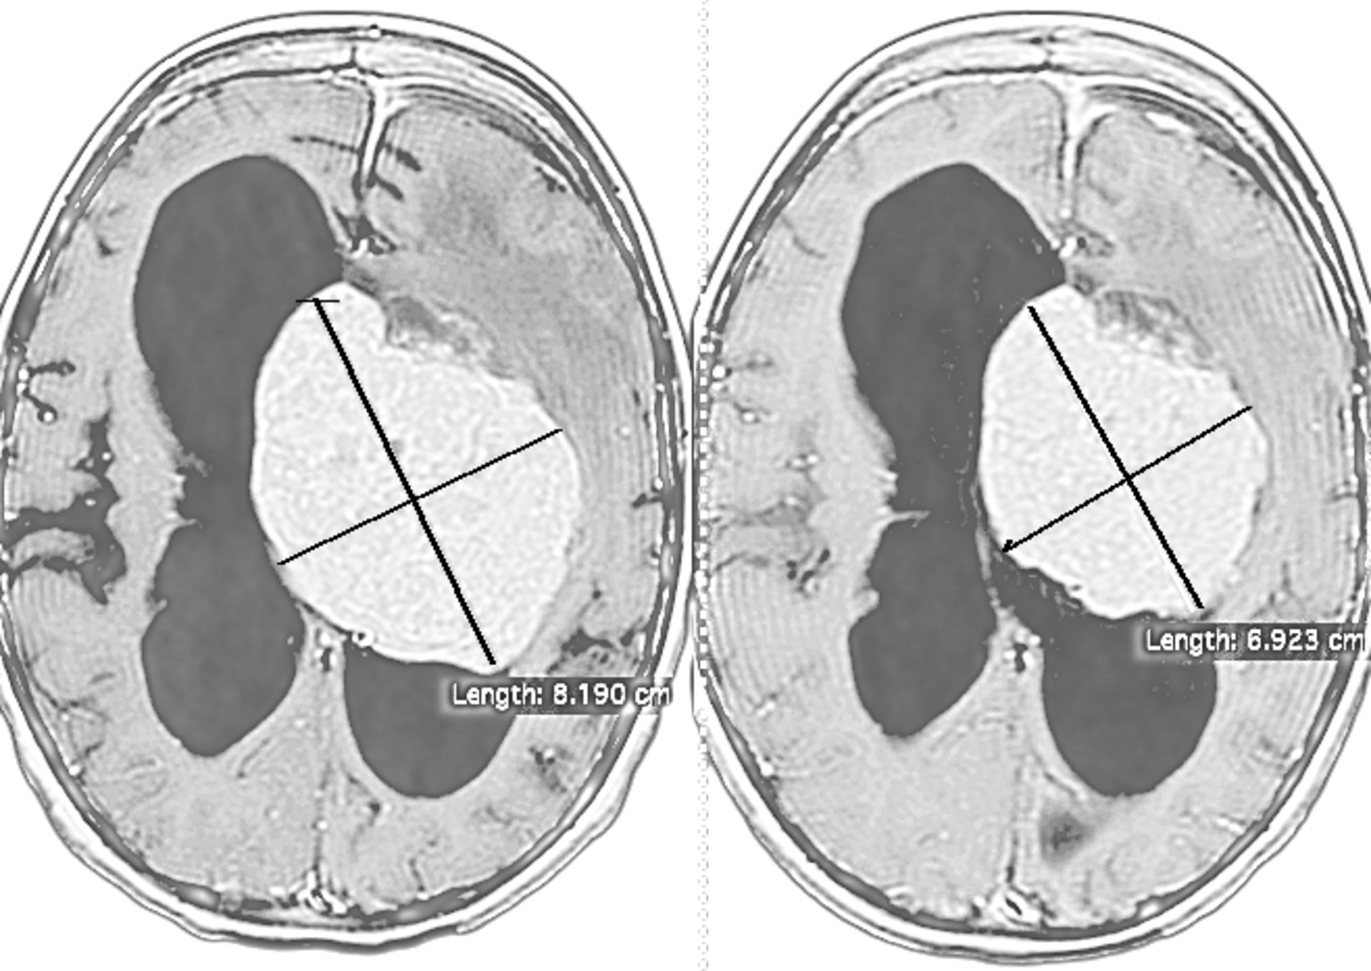
\includegraphics[scale=0.3]{fig/fig6.pdf}
		\caption{Exemplo de medida bidimensional (2D) em dois momentos, mostrando avaliação de resposta. Antes do tratamento, a lesão mediu $8,19 \times 6,2 cm = 50,8$, depois do tratamento, mediu $6,92 \times 5,5 cm = 38,1$. O cálculo da resposta é feito obtendo o produto dos maiores diâmetros perpendiculares e dividindo o valor posterior pelo valor anterior. $R = 38,1 \div 50,8 = 0,75$ Neste caso, ocorreu uma redução objetiva de 25\% pelo método 2D, o que autoriza a classificação da resposta como \textit{menor} (imagem do arquivo do autor, modificada com o programa Gimp 2.8.}
		%\label{Rotulo}
	\end{center}
\end{figure}

A imagem onde a(s) lesão(s) aparece(m) com maior tamanho deve ser escolhida. As medidas subsequentes devem ser realizadas sempre no mesmo plano (axial, sagital, coronal) e aproximadamente mesmo nível da imagem inicial. No exemplo da figura acima, o plano é axial e o nível é logo acima dos núcleos da base. A lesão de grandes proporções ocupa o ventrículo lateral direito e atravessa a linha média. A imagem pós-tratamento é nitidamente menor, mas essa redução precisa ser objetivamente quantificada. Escolhendo-se a imagem com maior área lesional no corte axial, mede-se os dois maiores diâmetros perpendiculares entre si. O produto destes diâmetros é uma estimativa do volume tumoral (método 2D). O método 2D tem maior acurácia na pediatria \cite{warren}.

A comparação entre os valores antes e após o tratamento mostra que ocorreu uma redução de 25\% do valor estimado para o tamanho tumoral. Esta magnitude de redução encontra-se no limite entre a ausência de mudança (doença estável) e uma mudança menos significativa (resposta menor), ilustrando como a inspeção visual e a avaliação quantitativa podem dar impressões subjetivas diferentes. A avaliação quantitativa da resposta é imprescindível para classificar adequadamente os pacientes e decidir a conduta clínica.


\chapter{Informações sobre as drogas utilizadas}

\section{Carboplatina}

Aprovada pela ANVISA para uso adulto. Sua utilização em crianças e adolescentes é não padronizada (\textit{off-label}). Indicações: carcinoma de ovário, carcinoma de pequenas células de pulmão, carcinomas espino-celulares de cabeça e pescoço e carcinomas de cérvice uterina. Outros usos, como no tratamento de tumores cerebrais, são não padronizados (\textit{off-label}). Contra-indicações: hipersensibilidade à droga ou outros constituintes da fórmula ou à cisplatina; insuficiência renal grave, mielodepressão grave e/ou na presença de sangramento volumoso. Não deve ser usada durante a gravidez e lactação (dados da bula aprovada epla ANVISA).

Seu mecanismo de ação é semelhante ao da cisplatina. Liga-se ao ADN em replicação causando quebras de fita simples e ligações cruzadas interfilamentares. \(\alpha t_\frac{1}{2}\) \footnote{Meia-vida de distribuição} e \(\beta t_\frac{1}{2}\) \footnote{Meia-vida de eliminação} são, respectivamente, 1,1 a 2 horas e 2,6 a 5,9 horas. Não liga-se a proteínas. Via de eliminação principal: renal. Precisa de ajuste de dose na insuficiência renal.

Toxicidade:
\renewcommand{\labelenumi}{\Alph{enumi}}
\begin{enumerate}
	\item Imediata: primeiras 24-48h. Comum (21-100\%): náuseas e vômitos. Ocasional (5-20\%): hipersensibilidade, constipação, diarreía. Raro (<5\%): rash, mucosite.
	\item Subaguda: 2-3 semanas. Comum: mielossupressão, distúrbios eletrolíticos. Ocasional: alteração de função hepática e/ou renal, dor abdominal, astenia. Raro: hiperbilirrubinemia.
	\item Retardada: qualquer momento após tratamento. Ocasional: ototoxicidade. Raro: alopécia, neuropatia periférica, amaurose noturna e/ou a cores; leucemia secundária.
\end{enumerate}

Formulação e estabilidade: 
		
Frascos de solução aquosa pré-diluída ou pó liofilizado para diluição, variando de 150 a 600 mg por frasco. Diluição padrão 10 mg/ml (checar disponibilidade). Checar apresentação sobre validade. Reconstituir em água para injeção, SG5\% ou SF0,9\% a 10mg/ml. Pode ser rediluída em SG5\% ou SF0,9\% até 0,5 mg/ml, permanencendo estável por até 8h a 25\(^\circ\) C. Alumínio reage com a carboplatina e pode causar sua precipitação. Evitar dispositivos de injeção com partes de alumínio. Proteger da luz.

\section{Cisplatina}

Aprovada pela ANVISA para uso adulto e pediátrico. Indicações: tumores metastáticos de testículo, tumores metastáticos de ovário, câncer avançado de bexiga, carcinomas espino-celulares de cabeça e pescoço. Outros usos, como no tratamento de tumores cerebrais, são não padronizados (\textit{off-label}). Contra-indicações: hipersensibilidade à droga ou a componentes da fórmula, mielodepressão, insuficiência renal grave, distúrbios de audição, infecções generalizadas. Não deve ser usada na gravidez ou lactação (dados da bula aprovada pela ANVISA). 

	Complexo inorgânico hidrossolúvel contendo um átomo central de platina, 2 átomos de cloro e 2 moléculas de amônia. Em solução aquosa, os átomos de cloro são lentamente deslocados para a solução, gerando um complexo hidratado positivamente carregado. Este complexo ativado reage com sítios nucleofílicos do ADN, ARN e proteínas, resultando na formação de ligações covalentes bifuncionais. As ligações cruzadas intrafilamentares entre citosina e guanina são as principais responsáveis pela inibição da síntese de ADN. Tem citotoxicidade sinérgica com radiação e outros agentes quimioterápicos. Sua distribuição é rápida (25-80 min) e sua meia-vida de eliminação é de 60-70 h. A platina (mas não a cisplatina em si) liga-se a proteínas plasmáticas (90\% três horas após injeção). A meia-vida de eliminação da platina ligada á albumina é de 5 dias ou mais. Pode-se encontrar platina nos tecidos até 180 dias após a última admisntração. A excreção é renal e a penetração no SNC é mínima.

Toxicidade:
\renewcommand{\labelenumi}{\Alph{enumi}}
\begin{enumerate}
	\item Imediata: primeiras 24-48h. Comum (21-100\%): náuseas e vômitos. Ocasional (5-20\%): sabor metálico. Raro (<5\%): anafilaxia, flebite, ulceração por extravasamento (se [] > 0,5 mg/ml).
	\item Subaguda: 2-3 semanas. Comum: mielossupressão, hipomagnesemia, perda auditiva de frequências altas, nefrotoxicidade. Ocasional: distúrbios eletrolíticos, neuropatia periférica. Raro: vestibulopatia, zumbido, rash, convulsões, disfunção hepática.
	\item Retardada: qualquer momento após tratamento. Ocasional: perda auditiva na faixa de frequências médias. Raro: arreflexia, perda da propriocepção e sensação vibratória, amaurose central, turvação visual, amaurose de cores, falência renal crônica, malignidade secundária.
	\item Outros: teratogênica em animais, excretada no leite materno.
\end{enumerate}

Formulação e estabilidade:

	Disponível em solução pré-diluída a 1 mg/ml de cisplatina e 9 mg/ml de cloreto de sódio. Armazenar a 15-25\(^\circ\) C. NÃO REFRIGERAR! Proteger da luz. Pode ser rediluída em SGF ou SF0,9\%, desde que a solução contenha > 0,2\% de NaCl. Soluções contendo dextrose, salina e/ou manitol são estáveis por 24-72h, porém não podem ser refrigeradas. Imcompatível com bicarbonato e soluções alcalinas. Alumínio reage com a cisplatina e pode causar sua precipitação. Evitar dispositivos de injeção com partes de alumínio. 

\appendix
\chapter{Quimioterapia de primeira linha}
\cleardoublepage

\section{Glioma de baixo grau}
{\let\thefootnote\relax\footnotetext{Versão Junho/2019}}
\textbf{Racional:} num estudo piloto, o grupo de Eric Bouffet mostrou a viabilidade e boa resposta do uso de vimblastina semanal em pacientes com reação à carboplatina. No estudo fase II do The Hospital for Sick Children, a vimblastina foi eficaz em induzir remissão parcial ou completa em 36\% de 51 pacientes com gliomas de baixo grau recorrentes ou progressivos, após esquemas prévios de quimioterapia e/ou radioterapia \cite{doi:10.1002/cncr.21091,doi:10.1200/JCO.2011.34.5843}. Um estudo fase II que incluiu 54 pacientes com gliomas de baixo grau progressivos usou a vimblastina como primeira linha, mostrando resultados aparentemente semelhantes a outros estudos (como o COG-A9952) \cite{lassaletta}. O protocolo original tratou os pacientes por 70 semanas. Nesta adaptação, os pacientes serão tratados por 1 ano (53 semanas), sendo opcional a prorrogação até completar 70 semanas de tratamento.

\textbf{Elegível:} astrocitoma de baixo grau (pilocítico, difuso, outros), oligodendroglioma, ganglioglioma, tumores mistos (oligoastrocitomas, outros), tumores de vias ópticas/hipotálamo (imagem típica, mesmo sem biópsia). Incluir tumores focais de tronco, excluir DIPG, ou tumores difusos de linha média H3K27M+. Pacientes com reação ou contraindicação ao uso de carboplatina; doença recorrente após prévio tratamento com quimioterapia e/ou radioterapia. Alternativa como primeira linha de tratamento. NÃO INICIAR ESTE PROTOCOLO EM CRIANÇAS GRAVEMENTE ENFERMAS.

\textbf{Alternativa:} a conduta expectante é uma opção, uma vez que, via de regra, o crescimento destes tumores é lento e sua progressão demora anos, ou mesmo décadas. Pacientes de maior risco, como aqueles com lesões de vias ópticas ou hipotálamo, síndrome diencefálica ou com lesões de crescimento rápido devem ser tratados sem grande demora. Se possível, uma nova ressecção cirúrgica deve ser avaliada. O protocolo baseado no estudo COG-A9952 (carboplatina e vincristina) pode ser usado como primeira linha. A principal alternativa adjuvante para pacientes com mais de 5 anos e sem NF-1 é a RT local. Pacientes com astrocitomas difusos têm maior risco de transformação maligna após RT.
%\begin{center}
%\begin{tikzpicture}
%  [node distance=.4cm, start chain=going right,]
%    \node[grande, ] (i) {indução};
%    \node[grande, ] (m) {manutenção};
%    \node[pequeno, below of=i, node distance=2cm] (cv) {cv};
%    \node[pequeno, join] (cv) {cv};
%    \node[pequeno, join] (cv) {cv};
%    \node[pequeno, join] (cv) {cv};
%    \node[pequeno, join] (cv) {cv};
%    \node[pequeno, join] (cv) {v};
%    \node[pequeno, join] (cv) {v};
%    \node[pequeno, join] (cv) {cv};
%    \node[pequeno, join] (cv) {cv};
%    \node[pequeno, join] (cv) {cv};
%    \node[pequeno, join] (cv) {cv};
%\end{tikzpicture}
%\end{center}
\cleardoublepage

\noindent{
\entrywithlabel[1\hsize]{\textbf{Nome}}\hfill
\\[0.3cm]
\entrywithlabel[.45\hsize]{\textbf{Peso}}\hfill  \entrywithlabel[.45\hsize]{\textbf{Estatura}}
}

\subsection{Quimioterapia adjuvante: 53 semanas ou 1 ano}
\begin{center}
\begin{table}[H]
\begin{tabular}{p{1,3cm}p{5,3cm}|p{4,7cm}|p{3cm}}
    \hline
    \multicolumn{1}{c|}{\multirow{2}{*}{\textbf{S1}}}&{Vimblastina \(6,0\)mg/m\(^2\)}&{Administrado: (  ) Sim (  ) Não}&{Rubrica}\\
    \multicolumn{1}{c|}{}&{EV em bolo (max 10mg)}&{Data:}&\\
    \hline
    {Exames:}&{Neut(\(>1,5\times10^3\)):}&{Plaq(\(>10^5\)):}&{TGO:}
    \\
    \hline
    \\
    \hline
    \multicolumn{1}{c|}{\multirow{2}{*}{\textbf{S2}}}&{Vimblastina \(6,0\)mg/m\(^2\)}&{Administrado: (  ) Sim (  ) Não}&{Rubrica}\\
    \multicolumn{1}{c|}{}&{EV em bolo (max 10mg)}&{Data:}&\\
    \hline
    \\
    \hline
    \multicolumn{1}{c|}{\multirow{2}{*}{\textbf{S3}}}&{Vimblastina \(6,0\)mg/m\(^2\)}&{Administrado: (  ) Sim (  ) Não}&{Rubrica}\\
    \multicolumn{1}{c|}{}&{EV em bolo (max 10mg)}&{Data:}&\\
    \hline
    \\
    \hline
    \multicolumn{1}{c|}{\multirow{2}{*}{\textbf{S4}}}&{Vimblastina \(6,0\)mg/m\(^2\)}&{Administrado: (  ) Sim (  ) Não}&{Rubrica}\\
    \multicolumn{1}{c|}{}&{EV em bolo (max 10mg)}&{Data:}&\\
    \hline
    \\
    \hline
    \multicolumn{1}{c|}{\multirow{2}{*}{\textbf{S5}}}&{Vimblastina \(6,0\)mg/m\(^2\)}&{Administrado: (  ) Sim (  ) Não}&{Rubrica}\\
    \multicolumn{1}{c|}{}&{EV em bolo (max 10mg)}&{Data:}&\\
    \hline
    {Exames:}&{Neut(\(>1,5\times10^3\)):}&{Plaq(\(>10^5\)):}&{TGO:}
    \\
    \hline\\
    \hline
    \multicolumn{1}{c|}{\multirow{2}{*}{\textbf{S6}}}&{Vimblastina \(6,0\)mg/m\(^2\)}&{Administrado: (  ) Sim (  ) Não}&{Rubrica}\\
    \multicolumn{1}{c|}{}&{EV em bolo (max 10mg)}&{Data:}&\\
    \hline
    \\
    \hline
    \multicolumn{1}{c|}{\multirow{2}{*}{\textbf{S7}}}&{Vimblastina \(6,0\)mg/m\(^2\)}&{Administrado: (  ) Sim (  ) Não}&{Rubrica}\\
    \multicolumn{1}{c|}{}&{EV em bolo (max 10mg)}&{Data:}&\\
    \hline
    \\
    \hline
    \multicolumn{1}{c|}{\multirow{2}{*}{\textbf{S8}}}&{Vimblastina \(6,0\)mg/m\(^2\)}&{Administrado: (  ) Sim (  ) Não}&{Rubrica}\\
    \multicolumn{1}{c|}{}&{EV em bolo (max 10mg)}&{Data:}&\\
    \hline
    \\
    \hline
    \multicolumn{1}{c|}{\multirow{2}{*}{\textbf{S9}}}&{Vimblastina \(6,0\)mg/m\(^2\)}&{Administrado: (  ) Sim (  ) Não}&{Rubrica}\\
    \multicolumn{1}{c|}{}&{EV em bolo (max 10mg)}&{Data:}&\\
    \hline
    {Exames:}&{Neut(\(>1,5\times10^3\)):}&{Plaq(\(>10^5\)):}&{TGO:}
    \\
    \hline
    \\
    \hline
    \multicolumn{1}{c|}{\multirow{2}{*}{\textbf{S10}}}&{Vimblastina \(6,0\)mg/m\(^2\)}&{Administrado: (  ) Sim (  ) Não}&{Rubrica}\\
    \multicolumn{1}{c|}{}&{EV em bolo (max 10mg)}&{Data:}&\\
    \hline
    \\
    \hline
    \multicolumn{1}{c|}{\multirow{2}{*}{\textbf{S11}}}&{Vimblastina \(6,0\)mg/m\(^2\)}&{Administrado: (  ) Sim (  ) Não}&{Rubrica}\\
    \multicolumn{1}{c|}{}&{EV em bolo (max 10mg)}&{Data:}&\\
    \hline
    \\
    \hline
    \multicolumn{1}{c|}{\multirow{2}{*}{\textbf{S12}}}&{Vimblastina \(6,0\)mg/m\(^2\)}&{Administrado: (  ) Sim (  ) Não}&{Rubrica}\\
    \multicolumn{1}{c|}{}&{EV em bolo (max 10mg)}&{Data:}&\\
    \hline
    \\
    \hline
    \multicolumn{1}{c|}{\multirow{2}{*}{\textbf{S13}}}&{Vimblastina \(6,0\)mg/m\(^2\)}&{Administrado: (  ) Sim (  ) Não}&{Rubrica}\\
    \multicolumn{1}{c|}{}&{EV em bolo (max 10mg)}&{Data:}&\\
    \hline
    {Exames:}&{Neut(\(>1,5\times10^3\)):}&{Plaq(\(>10^5\)):}&{TGO:}
    \\
    \hline
\end{tabular}
\end{table}
\begin{table}[H]
\begin{tabular}{p{1,3cm}p{5,3cm}|p{4,7cm}|p{3cm}}
    \hline
    \multicolumn{1}{c|}{\multirow{2}{*}{\textbf{S14}}}&{Vimblastina \(6,0\)mg/m\(^2\)}&{Administrado: (  ) Sim (  ) Não}&{Rubrica}\\
    \multicolumn{1}{c|}{}&{EV em bolo (max 10mg)}&{Data:}&\\
    \hline
    \\
    \hline
    \multicolumn{1}{c|}{\multirow{2}{*}{\textbf{S15}}}&{Vimblastina \(6,0\)mg/m\(^2\)}&{Administrado: (  ) Sim (  ) Não}&{Rubrica}\\
    \multicolumn{1}{c|}{}&{EV em bolo (max 10mg)}&{Data:}&\\
    \hline
    \\
    \hline
    \multicolumn{1}{c|}{\multirow{2}{*}{\textbf{S16}}}&{Vimblastina \(6,0\)mg/m\(^2\)}&{Administrado: (  ) Sim (  ) Não}&{Rubrica}\\
    \multicolumn{1}{c|}{}&{EV em bolo (max 10mg)}&{Data:}&\\
    \hline
    \\
     \hline
    \multicolumn{1}{c|}{\multirow{2}{*}{\textbf{S17}}}&{Vimblastina \(6,0\)mg/m\(^2\)}&{Administrado: (  ) Sim (  ) Não}&{Rubrica}\\
    \multicolumn{1}{c|}{}&{EV em bolo (max 10mg)}&{Data:}&\\
    \hline
    {Exames:}&{Neut(\(>1,5\times10^3\)):}&{Plaq(\(>10^5\)):}&{TGO:}
    \\
    \hline
    \\
    \hline
    \multicolumn{1}{c|}{\multirow{2}{*}{\textbf{S18}}}&{Vimblastina \(6,0\)mg/m\(^2\)}&{Administrado: (  ) Sim (  ) Não}&{Rubrica}\\
    \multicolumn{1}{c|}{}&{EV em bolo (max 10mg)}&{Data:}&\\
    \hline\\
    \hline
    \multicolumn{1}{c|}{\multirow{2}{*}{\textbf{S19}}}&{Vimblastina \(6,0\)mg/m\(^2\)}&{Administrado: (  ) Sim (  ) Não}&{Rubrica}\\
    \multicolumn{1}{c|}{}&{EV em bolo (max 10mg)}&{Data:}&\\
    \hline
    \\
    \hline
    \multicolumn{1}{c|}{\multirow{2}{*}{\textbf{S20}}}&{Vimblastina \(6,0\)mg/m\(^2\)}&{Administrado: (  ) Sim (  ) Não}&{Rubrica}\\
    \multicolumn{1}{c|}{}&{EV em bolo (max 10mg)}&{Data:}&\\
    \hline
    \\
    \hline
    \multicolumn{1}{c|}{\multirow{2}{*}{\textbf{S21}}}&{Vimblastina \(6,0\)mg/m\(^2\)}&{Administrado: (  ) Sim (  ) Não}&{Rubrica}\\
    \multicolumn{1}{c|}{}&{EV em bolo (max 10mg)}&{Data:}&\\
    \hline
    {Exames:}&{Neut(\(>1,5\times10^3\)):}&{Plaq(\(>10^5\)):}&{TGO:}
    \\
    \hline
    \\
    \hline
    \multicolumn{1}{c|}{\multirow{2}{*}{\textbf{S22}}}&{Vimblastina \(6,0\)mg/m\(^2\)}&{Administrado: (  ) Sim (  ) Não}&{Rubrica}\\
    \multicolumn{1}{c|}{}&{EV em bolo (max 10mg)}&{Data:}&\\
    \hline
    \\
    \hline
    \multicolumn{1}{c|}{\multirow{2}{*}{\textbf{S23}}}&{Vimblastina \(6,0\)mg/m\(^2\)}&{Administrado: (  ) Sim (  ) Não}&{Rubrica}\\
    \multicolumn{1}{c|}{}&{EV em bolo (max 10mg)}&{Data:}&\\
    \hline
    \\
    \hline
    \multicolumn{1}{c|}{\multirow{2}{*}{\textbf{S24}}}&{Vimblastina \(6,0\)mg/m\(^2\)}&{Administrado: (  ) Sim (  ) Não}&{Rubrica}\\
    \multicolumn{1}{c|}{}&{EV em bolo (max 10mg)}&{Data:}&\\
    \hline
    \\
    \hline
    \multicolumn{1}{c|}{\multirow{2}{*}{\textbf{S25}}}&{Vimblastina \(6,0\)mg/m\(^2\)}&{Administrado: (  ) Sim (  ) Não}&{Rubrica}\\
    \multicolumn{1}{c|}{}&{EV em bolo (max 10mg)}&{Data:}&\\
    \hline
    {Exames:}&{Neut(\(>1,5\times10^3\)):}&{Plaq(\(>10^5\)):}&{TGO:}
    \\
    \hline
    \\
    \hline
    \multicolumn{1}{c|}{\multirow{2}{*}{\textbf{S26}}}&{Vimblastina \(6,0\)mg/m\(^2\)}&{Administrado: (  ) Sim (  ) Não}&{Rubrica}\\
    \multicolumn{1}{c|}{}&{EV em bolo (max 10mg)}&{Data:}&\\
    \hline
    \multicolumn{4}{c}{Realizar imagem (RM) - não interromper protocolo aguardando resultado}
    \\
    \hline\\
    \hline
    \multicolumn{1}{c|}{\multirow{2}{*}{\textbf{S27}}}&{Vimblastina \(6,0\)mg/m\(^2\)}&{Administrado: (  ) Sim (  ) Não}&{Rubrica}\\
    \multicolumn{1}{c|}{}&{EV em bolo (max 10mg)}&{Data:}&\\
    \hline
    \\
    \hline
    \multicolumn{1}{c|}{\multirow{2}{*}{\textbf{S28}}}&{Vimblastina \(6,0\)mg/m\(^2\)}&{Administrado: (  ) Sim (  ) Não}&{Rubrica}\\
    \multicolumn{1}{c|}{}&{EV em bolo (max 10mg)}&{Data:}&\\
    \hline
\end{tabular}
\end{table}

\noindent{
\entrywithlabel[1\hsize]{\textbf{Nome}}\hfill
\\[0.3cm]
\entrywithlabel[.45\hsize]{\textbf{Peso}}\hfill  \entrywithlabel[.45\hsize]{\textbf{Estatura}}
}

\begin{table}[H]
\begin{tabular}{p{1,3cm}p{5,3cm}|p{4,7cm}|p{3cm}}
    \hline
    \multicolumn{1}{c|}{\multirow{2}{*}{\textbf{S29}}}&{Vimblastina \(6,0\)mg/m\(^2\)}&{Administrado: (  ) Sim (  ) Não}&{Rubrica}\\
    \multicolumn{1}{c|}{}&{EV em bolo (max 10mg)}&{Data:}&\\
    \hline
    {Exames:}&{Neut(\(>1,5\times10^3\)):}&{Plaq(\(>10^5\)):}&{TGO:}
    \\
    \hline
    \\
    \hline
    \multicolumn{1}{c|}{\multirow{2}{*}{\textbf{S30}}}&{Vimblastina \(6,0\)mg/m\(^2\)}&{Administrado: (  ) Sim (  ) Não}&{Rubrica}\\
    \multicolumn{1}{c|}{}&{EV em bolo (max 10mg)}&{Data:}&\\
    \hline
    \\
    \hline
    \multicolumn{1}{c|}{\multirow{2}{*}{\textbf{S31}}}&{Vimblastina \(6,0\)mg/m\(^2\)}&{Administrado: (  ) Sim (  ) Não}&{Rubrica}\\
    \multicolumn{1}{c|}{}&{EV em bolo (max 10mg)}&{Data:}&\\
    \hline
   \\
    \hline
    \multicolumn{1}{c|}{\multirow{2}{*}{\textbf{S32}}}&{Vimblastina \(6,0\)mg/m\(^2\)}&{Administrado: (  ) Sim (  ) Não}&{Rubrica}\\
    \multicolumn{1}{c|}{}&{EV em bolo (max 10mg)}&{Data:}&\\
    \hline
    \\
    \hline
    \multicolumn{1}{c|}{\multirow{2}{*}{\textbf{S33}}}&{Vimblastina \(6,0\)mg/m\(^2\)}&{Administrado: (  ) Sim (  ) Não}&{Rubrica}\\
    \multicolumn{1}{c|}{}&{EV em bolo (max 10mg)}&{Data:}&\\
    \hline
    {Exames:}&{Neut(\(>1,5\times10^3\)):}&{Plaq(\(>10^5\)):}&{TGO:}
    \\
    \hline
    \\
    \hline
    \multicolumn{1}{c|}{\multirow{2}{*}{\textbf{S34}}}&{Vimblastina \(6,0\)mg/m\(^2\)}&{Administrado: (  ) Sim (  ) Não}&{Rubrica}\\
    \multicolumn{1}{c|}{}&{EV em bolo (max 10mg)}&{Data:}&\\
    \hline
    \\
    \hline
    \multicolumn{1}{c|}{\multirow{2}{*}{\textbf{S35}}}&{Vimblastina \(6,0\)mg/m\(^2\)}&{Administrado: (  ) Sim (  ) Não}&{Rubrica}\\
    \multicolumn{1}{c|}{}&{EV em bolo (max 10mg)}&{Data:}&\\
    \hline
    \\
    \hline
    \multicolumn{1}{c|}{\multirow{2}{*}{\textbf{S36}}}&{Vimblastina \(6,0\)mg/m\(^2\)}&{Administrado: (  ) Sim (  ) Não}&{Rubrica}\\
    \multicolumn{1}{c|}{}&{EV em bolo (max 10mg)}&{Data:}&\\
    \hline
    \\
        \hline
    \multicolumn{1}{c|}{\multirow{2}{*}{\textbf{S37}}}&{Vimblastina \(6,0\)mg/m\(^2\)}&{Administrado: (  ) Sim (  ) Não}&{Rubrica}\\
    \multicolumn{1}{c|}{}&{EV em bolo (max 10mg)}&{Data:}&\\
    \hline
    {Exames:}&{Neut(\(>1,5\times10^3\)):}&{Plaq(\(>10^5\)):}&{TGO:}
    \\
    \hline
    \\
    \hline
    \multicolumn{1}{c|}{\multirow{2}{*}{\textbf{S38}}}&{Vimblastina \(6,0\)mg/m\(^2\)}&{Administrado: (  ) Sim (  ) Não}&{Rubrica}\\
    \multicolumn{1}{c|}{}&{EV em bolo (max 10mg)}&{Data:}&\\
    \hline
    \\
    \hline
    \multicolumn{1}{c|}{\multirow{2}{*}{\textbf{S39}}}&{Vimblastina \(6,0\)mg/m\(^2\)}&{Administrado: (  ) Sim (  ) Não}&{Rubrica}\\
    \multicolumn{1}{c|}{}&{EV em bolo (max 10mg)}&{Data:}&\\
   \hline
   \multicolumn{4}{c}{Realizar imagem (RM) - não interromper protocolo aguardando resultado}\\
    \hline
    \\
    \hline
    \multicolumn{1}{c|}{\multirow{2}{*}{\textbf{S40}}}&{Vimblastina \(6,0\)mg/m\(^2\)}&{Administrado: (  ) Sim (  ) Não}&{Rubrica}\\
    \multicolumn{1}{c|}{}&{EV em bolo (max 10mg)}&{Data:}&\\
    \hline
    \\
    \hline
    \multicolumn{1}{c|}{\multirow{2}{*}{\textbf{S41}}}&{Vimblastina \(6,0\)mg/m\(^2\)}&{Administrado: (  ) Sim (  ) Não}&{Rubrica}\\
    \multicolumn{1}{c|}{}&{EV em bolo (max 10mg)}&{Data:}&\\
    \hline
    {Exames:}&{Neut(\(>1,5\times10^3\)):}&{Plaq(\(>10^5\)):}&{TGO:}
    \\
    \hline
\end{tabular}
\end{table}
\begin{table}[H]
\begin{tabular}{p{1,3cm}p{5,3cm}|p{4,7cm}|p{3cm}}
        \hline
    \multicolumn{1}{c|}{\multirow{2}{*}{\textbf{S42}}}&{Vimblastina \(6,0\)mg/m\(^2\)}&{Administrado: (  ) Sim (  ) Não}&{Rubrica}\\
    \multicolumn{1}{c|}{}&{EV em bolo (max 10mg)}&{Data:}&\\
    \hline
    \\
    \hline
    \multicolumn{1}{c|}{\multirow{2}{*}{\textbf{S43}}}&{Vimblastina \(6,0\)mg/m\(^2\)}&{Administrado: (  ) Sim (  ) Não}&{Rubrica}\\
    \multicolumn{1}{c|}{}&{EV em bolo (max 10mg)}&{Data:}&\\
    \hline
    \\
    \hline
    \multicolumn{1}{c|}{\multirow{2}{*}{\textbf{S44}}}&{Vimblastina \(6,0\)mg/m\(^2\)}&{Administrado: (  ) Sim (  ) Não}&{Rubrica}\\
    \multicolumn{1}{c|}{}&{EV em bolo (max 10mg)}&{Data:}&\\
    \hline
    \\
    \hline
    \multicolumn{1}{c|}{\multirow{2}{*}{\textbf{S45}}}&{Vimblastina \(6,0\)mg/m\(^2\)}&{Administrado: (  ) Sim (  ) Não}&{Rubrica}\\
    \multicolumn{1}{c|}{}&{EV em bolo (max 10mg)}&{Data:}&\\
    \hline
    {Exames:}&{Neut(\(>1,5\times10^3\)):}&{Plaq(\(>10^5\)):}&{TGO:}
    \\
    \hline
    \\
    \hline
    \multicolumn{1}{c|}{\multirow{2}{*}{\textbf{S46}}}&{Vimblastina \(6,0\)mg/m\(^2\)}&{Administrado: (  ) Sim (  ) Não}&{Rubrica}\\
    \multicolumn{1}{c|}{}&{EV em bolo (max 10mg)}&{Data:}&\\
    \hline
   \\
    \hline
    \multicolumn{1}{c|}{\multirow{2}{*}{\textbf{S47}}}&{Vimblastina \(6,0\)mg/m\(^2\)}&{Administrado: (  ) Sim (  ) Não}&{Rubrica}\\
    \multicolumn{1}{c|}{}&{EV em bolo (max 10mg)}&{Data:}&\\
    \hline
    \\
    \hline
    \multicolumn{1}{c|}{\multirow{2}{*}{\textbf{S48}}}&{Vimblastina \(6,0\)mg/m\(^2\)}&{Administrado: (  ) Sim (  ) Não}&{Rubrica}\\
    \multicolumn{1}{c|}{}&{EV em bolo (max 10mg)}&{Data:}&\\
    \hline
    \\
    \hline
    \multicolumn{1}{c|}{\multirow{2}{*}{\textbf{S49}}}&{Vimblastina \(6,0\)mg/m\(^2\)}&{Administrado: (  ) Sim (  ) Não}&{Rubrica}\\
    \multicolumn{1}{c|}{}&{EV em bolo (max 10mg)}&{Data:}&\\
    \hline
    {Exames:}&{Neut(\(>1,5\times10^3\)):}&{Plaq(\(>10^5\)):}&{TGO:}
    \\
    \hline
    \\
    \hline
    \multicolumn{1}{c|}{\multirow{2}{*}{\textbf{S50}}}&{Vimblastina \(6,0\)mg/m\(^2\)}&{Administrado: (  ) Sim (  ) Não}&{Rubrica}\\
    \multicolumn{1}{c|}{}&{EV em bolo (max 10mg)}&{Data:}&\\
    \hline
    \\
    \hline
    \multicolumn{1}{c|}{\multirow{2}{*}{\textbf{S51}}}&{Vimblastina \(6,0\)mg/m\(^2\)}&{Administrado: (  ) Sim (  ) Não}&{Rubrica}\\
    \multicolumn{1}{c|}{}&{EV em bolo (max 10mg)}&{Data:}&\\
    \hline
    \\
    \hline
    \multicolumn{1}{c|}{\multirow{2}{*}{\textbf{S52}}}&{Vimblastina \(6,0\)mg/m\(^2\)}&{Administrado: (  ) Sim (  ) Não}&{Rubrica}\\
    \multicolumn{1}{c|}{}&{EV em bolo (max 10mg)}&{Data:}&\\
    \hline
    \\
    \hline
    \multicolumn{1}{c|}{\multirow{2}{*}{\textbf{S53}}}&{Vimblastina \(6,0\)mg/m\(^2\)}&{Administrado: (  ) Sim (  ) Não}&{Rubrica}\\
    \multicolumn{1}{c|}{}&{EV em bolo (max 10mg)}&{Data:}&\\
    \hline
    {Exames:}&{Neut(\(>1,5\times10^3\)):}&{Plaq(\(>10^5\)):}&{TGO:}
    \\
   \hline
\end{tabular}
\end{table}
\textbf{\textit{Final de Protocolo}}
\end{center}
\clearpage

\subsection{Sequência opcional - semanas 54 a 70}
\begin{center}

\noindent
\entrywithlabel[1\hsize]{\textbf{Nome}}\hfill
\\[0.3cm]
\entrywithlabel[.45\hsize]{\textbf{Peso}}\hfill  \entrywithlabel[.45\hsize]{\textbf{Estatura}}

\begin{table}[H]
\begin{tabular}{p{1,3cm}p{5,3cm}|p{4,7cm}|p{3cm}}
    \hline
    \multicolumn{1}{c|}{\multirow{2}{*}{\textbf{S54}}}&{Vimblastina \(6,0\)mg/m\(^2\)}&{Administrado: (  ) Sim (  ) Não}&{Rubrica}\\
    \multicolumn{1}{c|}{}&{EV em bolo (max 10mg)}&{Data:}&\\
    \hline
    {Exames:}&{Neut(\(>1,5\times10^3\)):}&{Plaq(\(>10^5\)):}&{TGO:}
    \\
    \hline
    \\
    \hline
    \multicolumn{1}{c|}{\multirow{2}{*}{\textbf{S55}}}&{Vimblastina \(6,0\)mg/m\(^2\)}&{Administrado: (  ) Sim (  ) Não}&{Rubrica}\\
    \multicolumn{1}{c|}{}&{EV em bolo (max 10mg)}&{Data:}&\\
   \\
    \hline
    \multicolumn{1}{c|}{\multirow{2}{*}{\textbf{S56}}}&{Vimblastina \(6,0\)mg/m\(^2\)}&{Administrado: (  ) Sim (  ) Não}&{Rubrica}\\
    \multicolumn{1}{c|}{}&{EV em bolo (max 10mg)}&{Data:}&\\
    \hline
    \\
    \hline
    \multicolumn{1}{c|}{\multirow{2}{*}{\textbf{S4}}}&{Vimblastina \(6,0\)mg/m\(^2\)}&{Administrado: (  ) Sim (  ) Não}&{Rubrica}\\
    \multicolumn{1}{c|}{}&{EV em bolo (max 10mg)}&{Data:}&\\
    \hline
    \\
    \hline
    \multicolumn{1}{c|}{\multirow{2}{*}{\textbf{S57}}}&{Vimblastina \(6,0\)mg/m\(^2\)}&{Administrado: (  ) Sim (  ) Não}&{Rubrica}\\
    \multicolumn{1}{c|}{}&{EV em bolo (max 10mg)}&{Data:}&\\
    \hline
    {Exames:}&{Neut(\(>1,5\times10^3\)):}&{Plaq(\(>10^5\)):}&{TGO:}
    \\
    \hline\\
    \hline
    \multicolumn{1}{c|}{\multirow{2}{*}{\textbf{S58}}}&{Vimblastina \(6,0\)mg/m\(^2\)}&{Administrado: (  ) Sim (  ) Não}&{Rubrica}\\
    \multicolumn{1}{c|}{}&{EV em bolo (max 10mg)}&{Data:}&\\
    \hline
    \\
    \hline
    \multicolumn{1}{c|}{\multirow{2}{*}{\textbf{S59}}}&{Vimblastina \(6,0\)mg/m\(^2\)}&{Administrado: (  ) Sim (  ) Não}&{Rubrica}\\
    \multicolumn{1}{c|}{}&{EV em bolo (max 10mg)}&{Data:}&\\
    \hline
    \\
    \hline
    \multicolumn{1}{c|}{\multirow{2}{*}{\textbf{S60}}}&{Vimblastina \(6,0\)mg/m\(^2\)}&{Administrado: (  ) Sim (  ) Não}&{Rubrica}\\
    \multicolumn{1}{c|}{}&{EV em bolo (max 10mg)}&{Data:}&\\
    \hline
    \\
    \hline
    \multicolumn{1}{c|}{\multirow{2}{*}{\textbf{S61}}}&{Vimblastina \(6,0\)mg/m\(^2\)}&{Administrado: (  ) Sim (  ) Não}&{Rubrica}\\
    \multicolumn{1}{c|}{}&{EV em bolo (max 10mg)}&{Data:}&\\
    \hline
    {Exames:}&{Neut(\(>1,5\times10^3\)):}&{Plaq(\(>10^5\)):}&{TGO:}
    \\
    \hline
    \\
    \hline
    \multicolumn{1}{c|}{\multirow{2}{*}{\textbf{S62}}}&{Vimblastina \(6,0\)mg/m\(^2\)}&{Administrado: (  ) Sim (  ) Não}&{Rubrica}\\
    \multicolumn{1}{c|}{}&{EV em bolo (max 10mg)}&{Data:}&\\
    \hline
    \\
    \hline
    \multicolumn{1}{c|}{\multirow{2}{*}{\textbf{S63}}}&{Vimblastina \(6,0\)mg/m\(^2\)}&{Administrado: (  ) Sim (  ) Não}&{Rubrica}\\
    \multicolumn{1}{c|}{}&{EV em bolo (max 10mg)}&{Data:}&\\
    \hline
    \\
    \hline
    \multicolumn{1}{c|}{\multirow{2}{*}{\textbf{S64}}}&{Vimblastina \(6,0\)mg/m\(^2\)}&{Administrado: (  ) Sim (  ) Não}&{Rubrica}\\
    \multicolumn{1}{c|}{}&{EV em bolo (max 10mg)}&{Data:}&\\
    \hline
    \\
    \hline
    \multicolumn{1}{c|}{\multirow{2}{*}{\textbf{S65}}}&{Vimblastina \(6,0\)mg/m\(^2\)}&{Administrado: (  ) Sim (  ) Não}&{Rubrica}\\
    \multicolumn{1}{c|}{}&{EV em bolo (max 10mg)}&{Data:}&\\
    \hline
    {Exames:}&{Neut(\(>1,5\times10^3\)):}&{Plaq(\(>10^5\)):}&{TGO:}
    \\
    \hline
\end{tabular}
\end{table}
\begin{table}[H]
\begin{tabular}{p{1,3cm}p{5,3cm}|p{4,7cm}|p{3cm}}
    \hline
    \multicolumn{1}{c|}{\multirow{2}{*}{\textbf{S66}}}&{Vimblastina \(6,0\)mg/m\(^2\)}&{Administrado: (  ) Sim (  ) Não}&{Rubrica}\\
    \multicolumn{1}{c|}{}&{EV em bolo (max 10mg)}&{Data:}&\\
    \hline\\
    \hline
    \multicolumn{1}{c|}{\multirow{2}{*}{\textbf{S67}}}&{Vimblastina \(6,0\)mg/m\(^2\)}&{Administrado: (  ) Sim (  ) Não}&{Rubrica}\\
    \multicolumn{1}{c|}{}&{EV em bolo (max 10mg)}&{Data:}&\\
    \hline\\
    \hline
    \multicolumn{1}{c|}{\multirow{2}{*}{\textbf{S68}}}&{Vimblastina \(6,0\)mg/m\(^2\)}&{Administrado: (  ) Sim (  ) Não}&{Rubrica}\\
    \multicolumn{1}{c|}{}&{EV em bolo (max 10mg)}&{Data:}&\\
    \hline
    \\
     \hline
    \multicolumn{1}{c|}{\multirow{2}{*}{\textbf{S69}}}&{Vimblastina \(6,0\)mg/m\(^2\)}&{Administrado: (  ) Sim (  ) Não}&{Rubrica}\\
    \multicolumn{1}{c|}{}&{EV em bolo (max 10mg)}&{Data:}&\\
    \hline
    {Exames:}&{Neut(\(>1,5\times10^3\)):}&{Plaq(\(>10^5\)):}&{TGO:}
    \\
    \hline\\
    \hline
    \multicolumn{1}{c|}{\multirow{2}{*}{\textbf{S70}}}&{Vimblastina \(6,0\)mg/m\(^2\)}&{Administrado: (  ) Sim (  ) Não}&{Rubrica}\\
    \multicolumn{1}{c|}{}&{EV em bolo (max 10mg)}&{Data:}&\\
    \hline
\end{tabular}
\end{table}
\textbf{\textit{Final de Protocolo}}

\textbf{Solicitar imagem (RNM)}
\end{center}
\subsection{Modificações de dose:}
O protocolo original requeria uma dose semanal de vimblastina, com uma tolerância de dois dias a mais ou a menos. Atrasos frequentes ou muito maiores que isso podem reduzir de forma imprevisível a eficácia do tratamento. Em pacientes com \(SC < 0,6 m^2\), as doses devem ser calculadas de acordo com o peso: 

\[\frac{dose/m^2 \times peso(kg)}{30}\] 

Se a contagem de neutrófilos for $< 750/mm^3$, porém $\geq 500/mm^3$, reduzir dose para $5 mg/m^2$ ou 80\% da dose se $SC < 0,6 m^2$. Se a contagem de neutrófilos for $< 500mm^3$, interromper até subir para $\geq 750/mm^2$. Se toxicidade hematológica recorrente, reduzir dose para $4 mg/m^2$ ou 67\% da dose se $SC < 0,6 m^2$. No protocolo original, não foram permitidos fatores de crescimento.

\subsection{Avaliação de resposta:}

Uma ressonância magnética (RM) realizada com até 1 mês de antecedência foi exigida para iniciar o protocolo original. As imagens subsequentes foram realizadas nas semanas 26, 39, 52 e 70 após o início do protocolo. Todas as imagens de RM devem incluir obrigatoriamente as sequências T1, T2, FLAIR e T1 com contraste. O critério de resposta da OMS deve ser utilizado conforme descrito anteriormente.

\subsection{Avaliação no seguimento:}

Para os pacientes que completaram o protocolo, uma imagem de RM deve ser solicitada a cada 3 meses no primeiro ano, a cada 6 seis meses no segundo ano e, depois, anualmente por 5 anos. 

\textbf{ATENÇÃO:} o objetivo deste protocolo é ADIAR O USO DA RT (se não tiver sido feita) até a criança atingir uma idade onde os efeitos adversos da radiação sejam reduzidos, ou controlar doença recidivada após a RT. A principal resposta deste protocolo é ESTABILIZAÇÃO DA DOENÇA. Logo, é inadequado iniciar este esquema de QT em crianças em regime de internação prolongada, dependentes de cuidados hospitalares, visando "melhorar" sua condição clínica. Igualmente, é inadequado iniciar este protocolo em crianças com risco de complicações graves, como naquelas que têm sequelas importantes e muito limitantes.

\cleardoublepage
\section{Meduloblastoma - Risco padrão -- Adaptado dos ensaios CCG-9961 e ACNS0331}
{\let\thefootnote\relax\footnotetext{Versão Junho/2019}}
\textbf{Racional:} no estudo CCG-9961 do COG, a adição de QT permitiu a redução da dose da RT para o neuro-eixo para 2340 cGY, com \textit{boost} para o sítio tumoral completando 54 Gy de dose total\cite{4980}. O COG testou recentemente uma nova redução da RT, com o ensaio fase III ACNS0331, o qual foi interrompido precocemente devido a excesso de recidivas no grupo experimental. Dessa forma, a recomendação é de manter a dose atual de RT para meduloblastomas de risco padrão.\cite{Michalski2016} O COG fez modificações na manutenção do protocolo. Utilizamos o esquema de QT segundo o braço controle do ensaio ACNS0331, derivado do CCG-9961.

\textbf{Elegível:} apenas meduloblastoma (fossa posterior), com menos de 1,5cm\textsuperscript{2} de tumor residual (RNM de controle até 21 dias pós-op, preferido 72h após); sem metástases (RNM de neuro-eixo e PL/MO); excluir tumores com anaplasia ou positivos para N-MYC/C-MYC. Tratamento precisa iniciar até 31 dias após cirurgia. Excluir pacientes com menos de 3 anos. NÃO INICIAR ESTE PROTOCOLO EM CRIANÇAS GRAVEMENTE ENFERMAS.

\textbf{Alternativa:} a principal alternativa é a RT para neuro-eixo sem redução de dose (36 Gy) com boost para a fossa posterior de 18-20 Gy, completando 54-56 Gy de dose total. Essa estratégia, na ausência de QT adjuvante, é capaz de evitar recidivas em pacientes de risco padrão.
\cleardoublepage
\noindent
\entrywithlabel[1\hsize]{\textbf{Nome}}\hfill
\\[0.3cm]
\entrywithlabel[.45\hsize]{\textbf{Peso}}\hfill  \entrywithlabel[.45\hsize]{\textbf{Estatura}}

\subsection{Radioquimioterapia: 7 semanas (43 dias)}

\begin{center}
\begin{tabular}{p{1cm}p{2cm}|p{2cm}|p{1cm}|p{4cm}|p{3cm}}
	\hline
	\multicolumn{6}{c}{\textbf{SEMANA 1}}\\
\hline
    \multicolumn{1}{c|}{\multirow{2}{*}{\textbf{Dia}}}&\multicolumn{2}{c|}{Dose RT}&\multicolumn{1}{c|}{\multirow{2}{*}{Data}}&\multicolumn{1}{c|}{\multirow{2}{*}{Quimioterapia}}&\multicolumn{1}{c}{\multirow{2}{*}{Rubrica}} \\
    \cline{2-3}
    \multicolumn{1}{c|}{\multirow{1}{*}{}}&{Neuro-eixo}&{Fossa poster}&& \\
	\hline
	\multicolumn{1}{c|}{\multirow{1}{*}{\textbf{D1}}}&\multicolumn{1}{c|}{}&{\(1,8\) Gy}&&{Vincristina \(1,5\) mg/m\(^2\)}&\\
    \multicolumn{1}{c|}{\multirow{1}{*}{\textbf{D2}}}&\multicolumn{1}{c|}{}&{\(1,8\) Gy}&&{}&\\
    \multicolumn{1}{c|}{\multirow{1}{*}{\textbf{D3}}}&\multicolumn{1}{c|}{}&{\(1,8\) Gy}&&{}&\\
    \multicolumn{1}{c|}{\multirow{1}{*}{\textbf{D4}}}&\multicolumn{1}{c|}{}&{\(1,8\) Gy}&&{}&\\
    \multicolumn{1}{c|}{\multirow{1}{*}{\textbf{D5}}}&\multicolumn{1}{c|}{}&{\(1,8\) Gy}&&{}&\\
    \hline
    \multicolumn{1}{c|}{\multirow{2}{*}{\textbf{Exames}}}&\multicolumn{2}{l|}{Neut (\(>7,5\times10^2\)):}&\multicolumn{2}{l|}{Plaq (\(>7,5\times10^4\)):}&\\
    \cline{2-6}
    \multicolumn{1}{c|}{\multirow{2}{*}{{}}}&\multicolumn{2}{l|}{BT(<1,9mg/dl):}&\multicolumn{2}{l|}{BD(\(<1,5\)mg/dl):}&
    \\
    \hline
\end{tabular}
\begin{table}[H]
\begin{tabular}{p{1cm}p{2cm}|p{2cm}|p{1cm}|p{4cm}|p{3cm}}
	\hline
	\multicolumn{6}{c}{\textbf{SEMANA 2}}\\
\hline
    \multicolumn{1}{c|}{\multirow{2}{*}{\textbf{Dia}}}&\multicolumn{2}{c|}{Dose RT}&\multicolumn{1}{c|}{\multirow{2}{*}{Data}}&\multicolumn{1}{c|}{\multirow{2}{*}{Quimioterapia}}&\multicolumn{1}{c}{\multirow{2}{*}{Rubrica}} \\
    \cline{2-3}
    \multicolumn{1}{c|}{\multirow{1}{*}{}}&{Neuro-eixo}&{Fossa poster}&& \\
	\hline
	\multicolumn{1}{c|}{\multirow{1}{*}{\textbf{D8}}}&\multicolumn{1}{c|}{}&{\(1,8\) Gy}&&{Vincristina \(1,5\) mg/m\(^2\)}&\\
    \multicolumn{1}{c|}{\multirow{1}{*}{\textbf{D9}}}&\multicolumn{1}{c|}{}&{\(1,8\) Gy}&&{}&\\
    \multicolumn{1}{c|}{\multirow{1}{*}{\textbf{D10}}}&\multicolumn{1}{c|}{}&{\(1,8\) Gy}&&{}&\\
    \multicolumn{1}{c|}{\multirow{1}{*}{\textbf{D11}}}&\multicolumn{1}{c|}{}&{\(1,8\) Gy}&&{}&\\
    \multicolumn{1}{c|}{\multirow{1}{*}{\textbf{D12}}}&\multicolumn{1}{c|}{}&{\(1,8\) Gy}&&{}&\\
    \hline
    \multicolumn{1}{c|}{\multirow{2}{*}{\textbf{Exames}}}&\multicolumn{2}{l|}{Neut (\(>7,5\times10^2\)):}&\multicolumn{2}{l|}{Plaq (\(>7,5\times10^4\)):}&\\
    \cline{2-6}
    \multicolumn{1}{c|}{\multirow{2}{*}{{}}}&\multicolumn{2}{l|}{BT(<1,9mg/dl):}&\multicolumn{2}{l|}{BD(\(<1,5\)mg/dl):}&
    \\
    \hline
\end{tabular}
\end{table}
\begin{table}[H]
\begin{tabular}{p{1cm}p{2cm}|p{2cm}|p{1cm}|p{4cm}|p{3cm}}
	\hline
	\multicolumn{6}{c}{\textbf{SEMANA 3}}\\
\hline
    \multicolumn{1}{c|}{\multirow{2}{*}{\textbf{Dia}}}&\multicolumn{2}{c|}{Dose RT}&\multicolumn{1}{c|}{\multirow{2}{*}{Data}}&\multicolumn{1}{c|}{\multirow{2}{*}{Quimioterapia}}&\multicolumn{1}{c}{\multirow{2}{*}{Rubrica}} \\
    \cline{2-3}
    \multicolumn{1}{c|}{\multirow{1}{*}{}}&{Neuro-eixo}&{Fossa poster}&& \\
	\hline
	\multicolumn{1}{c|}{\multirow{1}{*}{\textbf{D15}}}&\multicolumn{1}{c|}{}&{\(1,8\) Gy}&&{Vincristina \(1,5\) mg/m\(^2\)}&\\
    \multicolumn{1}{c|}{\multirow{1}{*}{\textbf{D16}}}&\multicolumn{1}{c|}{}&{\(1,8\) Gy}&&{}&\\    \multicolumn{1}{c|}{\multirow{1}{*}{\textbf{D17}}}&\multicolumn{1}{c|}{}&{\(1,8\) Gy}&&{}&\\
    \multicolumn{1}{c|}{\multirow{1}{*}{\textbf{D18}}}&\multicolumn{1}{c|}{}&{\(1,8\) Gy}&&{}&\\
    \multicolumn{1}{c|}{\multirow{1}{*}{\textbf{D19}}}&\multicolumn{1}{c|}{}&{\(1,8\) Gy}&&{}&\\
    \hline
    \multicolumn{1}{c|}{\multirow{2}{*}{\textbf{Exames}}}&\multicolumn{2}{l|}{Neut (\(>7,5\times10^2\)):}&\multicolumn{2}{l|}{Plaq (\(>7,5\times10^4\)):}&\\
    \cline{2-6}
    \multicolumn{1}{c|}{\multirow{2}{*}{{}}}&\multicolumn{2}{l|}{BT(<1,9mg/dl):}&\multicolumn{2}{l|}{BD(\(<1,5\)mg/dl):}&
    \\
    \hline
\end{tabular}
\end{table}
\begin{table}[H]
\begin{tabular}{p{1cm}p{2cm}|p{2cm}|p{1cm}|p{4cm}|p{3cm}}
	\hline
	\multicolumn{6}{c}{\textbf{SEMANA 4}}\\
\hline
    \multicolumn{1}{c|}{\multirow{2}{*}{\textbf{Dia}}}&\multicolumn{2}{c|}{Dose RT}&\multicolumn{1}{c|}{\multirow{2}{*}{Data}}&\multicolumn{1}{c|}{\multirow{2}{*}{Quimioterapia}}&\multicolumn{1}{c}{\multirow{2}{*}{Rubrica}} \\
    \cline{2-3}
    \multicolumn{1}{c|}{\multirow{1}{*}{}}&{Neuro-eixo}&{Fossa poster}&& \\
	\hline
	\multicolumn{1}{c|}{\multirow{1}{*}{\textbf{D22}}}&\multicolumn{1}{c|}{}&{\(1,8\) Gy}&&{Vincristina \(1,5\) mg/m\(^2\)}&\\
    \multicolumn{1}{c|}{\multirow{1}{*}{\textbf{D23}}}&\multicolumn{1}{c|}{}&{\(1,8\) Gy}&&{}&\\
    \multicolumn{1}{c|}{\multirow{1}{*}{\textbf{D24}}}&\multicolumn{1}{c|}{}&{\(1,8\) Gy}&&{}&\\
    \multicolumn{1}{c|}{\multirow{1}{*}{\textbf{D25}}}&\multicolumn{1}{c|}{\(1,8\) Gy}&&&{}&\\
    \multicolumn{1}{c|}{\multirow{1}{*}{\textbf{D26}}}&\multicolumn{1}{c|}{\(1,8\) Gy}&&&{}&\\
    \hline
    \multicolumn{1}{c|}{\multirow{2}{*}{\textbf{Exames}}}&\multicolumn{2}{l|}{Neut (\(>7,5\times10^2\)):}&\multicolumn{2}{l|}{Plaq (\(>7,5\times10^4\)):}&\\
    \cline{2-6}
    \multicolumn{1}{c|}{\multirow{2}{*}{{}}}&\multicolumn{2}{l|}{BT(<1,9mg/dl):}&\multicolumn{2}{l|}{BD(\(<1,5\)mg/dl):}&
    \\
    \hline
\end{tabular}
\end{table}
\begin{table}[H]
\begin{tabular}{p{1cm}p{2cm}|p{2cm}|p{1cm}|p{4cm}|p{3cm}}
	\hline
	\multicolumn{6}{c}{\textbf{SEMANA 5}}\\
\hline
    \multicolumn{1}{c|}{\multirow{2}{*}{\textbf{Dia}}}&\multicolumn{2}{c|}{Dose RT}&\multicolumn{1}{c|}{\multirow{2}{*}{Data}}&\multicolumn{1}{c|}{\multirow{2}{*}{Quimioterapia}}&\multicolumn{1}{c}{\multirow{2}{*}{Rubrica}} \\
    \cline{2-3}
    \multicolumn{1}{c|}{\multirow{1}{*}{}}&{Neuro-eixo}&{Fossa poster}&& \\
	\hline
	\multicolumn{1}{c|}{\multirow{1}{*}{\textbf{D29}}}&\multicolumn{1}{c|}{\(1,8\) Gy}&&&{Vincristina \(1,5\) mg/m\(^2\)}&\\
    \multicolumn{1}{c|}{\multirow{1}{*}{\textbf{D30}}}&\multicolumn{1}{c|}{\(1,8\) Gy}&&&{}&\\
    \multicolumn{1}{c|}{\multirow{1}{*}{\textbf{D31}}}&\multicolumn{1}{c|}{\(1,8\) Gy}&&&{}&\\
    \multicolumn{1}{c|}{\multirow{1}{*}{\textbf{D32}}}&\multicolumn{1}{c|}{\(1,8\) Gy}&&&{}&\\
    \multicolumn{1}{c|}{\multirow{1}{*}{\textbf{D33}}}&\multicolumn{1}{c|}{\(1,8\) Gy}&&&{}&\\
    \hline
    \multicolumn{1}{c|}{\multirow{2}{*}{\textbf{Exames}}}&\multicolumn{2}{l|}{Neut (\(>7,5\times10^2\)):}&\multicolumn{2}{l|}{Plaq (\(>7,5\times10^4\)):}&\\
    \cline{2-6}
    \multicolumn{1}{c|}{\multirow{2}{*}{{}}}&\multicolumn{2}{l|}{BT(<1,9mg/dl):}&\multicolumn{2}{l|}{BD(\(<1,5\)mg/dl):}&
    \\
    \hline
\end{tabular}
\end{table}
\begin{table}[H]
\begin{tabular}{p{1cm}p{2cm}|p{2cm}|p{1cm}|p{4cm}|p{3cm}}
	\hline
	\multicolumn{6}{c}{\textbf{SEMANA 6}}\\
\hline
    \multicolumn{1}{c|}{\multirow{2}{*}{\textbf{Dia}}}&\multicolumn{2}{c|}{Dose RT}&\multicolumn{1}{c|}{\multirow{2}{*}{Data}}&\multicolumn{1}{c|}{\multirow{2}{*}{Quimioterapia}}&\multicolumn{1}{c}{\multirow{2}{*}{Rubrica}} \\
    \cline{2-3}
    \multicolumn{1}{c|}{\multirow{1}{*}{}}&{Neuro-eixo}&{Fossa poster}&& \\
	\hline
	\multicolumn{1}{c|}{\multirow{1}{*}{\textbf{D36}}}&\multicolumn{1}{c|}{\(1,8\) Gy}&&&{Vincristina \(1,5\) mg/m\(^2\)}&\\
    \multicolumn{1}{c|}{\multirow{1}{*}{\textbf{D37}}}&\multicolumn{1}{c|}{\(1,8\) Gy}&&&{}&\\
    \multicolumn{1}{c|}{\multirow{1}{*}{\textbf{D38}}}&\multicolumn{1}{c|}{\(1,8\) Gy}&&&{}&\\
    \multicolumn{1}{c|}{\multirow{1}{*}{\textbf{D39}}}&\multicolumn{1}{c|}{\(1,8\) Gy}&&&{}&\\
    \multicolumn{1}{c|}{\multirow{1}{*}{\textbf{D40}}}&\multicolumn{1}{c|}{\(1,8\) Gy}&&&{}&\\
    \hline
    \multicolumn{1}{c|}{\multirow{2}{*}{\textbf{Exames}}}&\multicolumn{2}{l|}{Neut (\(>7,5\times10^2\)):}&\multicolumn{2}{l|}{Plaq (\(>7,5\times10^4\)):}&\\
    \cline{2-6}
    \multicolumn{1}{c|}{\multirow{2}{*}{{}}}&\multicolumn{2}{l|}{BT(<1,9mg/dl):}&\multicolumn{2}{l|}{BD(\(<1,5\)mg/dl):}&
    \\
    \hline
\end{tabular}
\end{table}

\pagebreak
\noindent
\entrywithlabel[1\hsize]{\textbf{Nome}}\hfill
\\[0.3cm]
\entrywithlabel[.45\hsize]{\textbf{Peso}}\hfill  \entrywithlabel[.45\hsize]{\textbf{Estatura}}

\begin{table}[H]
\begin{tabular}{p{1cm}p{2cm}|p{2cm}|p{1cm}|p{4cm}|p{3cm}}
	\hline
	\multicolumn{6}{c}{\textbf{SEMANA 7}}\\
\hline
    \multicolumn{1}{c|}{\multirow{2}{*}{\textbf{Dia}}}&\multicolumn{2}{c|}{Dose RT}&\multicolumn{1}{c|}{\multirow{2}{*}{Data}}&\multicolumn{1}{c|}{\multirow{2}{*}{Quimioterapia}}&\multicolumn{1}{c}{\multirow{2}{*}{Rubrica}} \\
    \cline{2-3}
    \multicolumn{1}{c|}{\multirow{1}{*}{}}&{Neuro-eixo}&{Fossa poster}&& \\
	\hline
	\multicolumn{1}{c|}{\multirow{1}{*}{\textbf{D43}}}&\multicolumn{1}{c|}{\(1,8\) Gy}&&&{Vincristina \(1,5\) mg/m\(^2\)}&\\
    \hline
    \multicolumn{1}{c|}{\multirow{2}{*}{\textbf{Exames}}}&\multicolumn{2}{l|}{Neut (\(>7,5\times10^2\)):}&\multicolumn{2}{l|}{Plaq (\(>7,5\times10^4\)):}&\\
    \cline{2-6}
    \multicolumn{1}{c|}{\multirow{2}{*}{{}}}&\multicolumn{2}{l|}{BT(<1,9mg/dl):}&\multicolumn{2}{l|}{BD(\(<1,5\)mg/dl):}&
    \\
    \hline
\end{tabular}
\end{table}
\textbf{Intervalo de 28 dias}\\
\end{center}
\textbf{Máximo de 8 doses de VCR, máximo de 20 dias recebendo RT cranioespinhal, máximo de 51 dias de RT no total}

\subsection{Manutenção: 04 ciclos A e 04 ciclos B}

\begin{center}
\begin{table}[H]
\begin{tabular}{p{1cm}p{6cm}|p{1cm}|p{3cm}|p{2.5cm}}
	\hline
	\multicolumn{5}{c}{\textbf{CICLO A}}\\
\hline
    \multicolumn{1}{c|}{\multirow{1}{*}{\textbf{Dia}}}&{Dose}&{Data}&{Administrado}&{Rubrica} \\
    \hline
    \multicolumn{1}{c|}{\multirow{1}{*}{\textbf{D71}}}&{Cisplatina \(75\) mg/m\(^2\) EV em 6h}&&{(  ) Sim (  ) Não}&\\
    \multicolumn{1}{c|}{\multirow{1}{*}{\textbf{D72}}}&{Vincristina \(1,5\) mg/m\(^2\), max \(2\) mg}&&{(  ) Sim (  ) Não}&\\
    \multicolumn{1}{c|}{\multirow{1}{*}{\textbf{}}}&&&&\\
    \hline
    \multicolumn{1}{c|}{\multirow{2}{*}{\textbf{Exames}}}&\multicolumn{2}{l|}{Neut(\(>10^3\)):}&{Plaq(\(>10^5\)):}&\\
    \cline{2-5}
    \multicolumn{1}{c|}{\multirow{2}{*}{{}}}&\multicolumn{2}{l|}{ClearCreat (\(>75\%\)) basal:}&{}&{}\\
    \hline
    \\
    \hline
    \multicolumn{1}{c|}{\multirow{1}{*}{\textbf{D78}}}&{Vincristina \(1,5\) mg/m\(^2\), max \(2\) mg}&&{(  ) Sim (  ) Não}&\\
    \hline
    \\
    \hline
    \multicolumn{1}{c|}{\multirow{1}{*}{\textbf{D85}}}&{Vincristina \(1,5\) mg/m\(^2\), max \(2\) mg}&&{(  ) Sim (  ) Não}&\\
    \hline
    \end{tabular}
    \end{table}
    \textbf{Intervalo de 28 dias}
   \begin{table}[H]
    \begin{tabular}{p{1cm}p{6cm}|p{1cm}|p{3cm}|p{2.5cm}}
    \hline
	\multicolumn{5}{c}{\textbf{CICLO B}}\\
	\hline
    \multicolumn{1}{c|}{\multirow{1}{*}{\textbf{Dia}}}&{Dose}&{Data}&{Administrado}&{Rubrica} \\
    \hline
    \multicolumn{1}{c|}{\multirow{1}{*}{\textbf{D113}}}&{Ciclofosfamida \(1,0\) g/m\(^2\) EV em 6h}&&{(  ) Sim (  ) Não}&\\
    \multicolumn{1}{c|}{\multirow{1}{*}{\textbf{D114}}}&{Ciclofosfamida \(1,0\) g/m\(^2\) EV em 6h}&&{(  ) Sim (  ) Não}&\\
    \multicolumn{1}{c|}{\multirow{1}{*}{\textbf{}}}&{Vincristina \(1,5\) mg/m\(^2\), max \(2\) mg}&&{(  ) Sim (  ) Não}&\\
    \hline
    \multicolumn{1}{c|}{\multirow{2}{*}{\textbf{Exames}}}&\multicolumn{2}{l|}{Neut(\(>10^3\)):}&{Plaq(\(>10^5\)):}&\\
    \cline{2-5}
    \multicolumn{1}{c|}{\multirow{2}{*}{{}}}&\multicolumn{2}{l|}{ClearCreat (\(>75\%\)) basal:}&{}&{}\\
    \hline
    \\
    \hline
    \multicolumn{1}{c|}{\multirow{1}{*}{\textbf{D120}}}&{Vincristina \(1,5\) mg/m\(^2\), max \(2\) mg}&&{(  ) Sim (  ) Não}&\\
    \hline
\end{tabular}
\end{table}
\textbf{Intervalo de 21 dias}
\begin{table}[H]
\begin{tabular}{p{1cm}p{6cm}|p{1cm}|p{3cm}|p{2.5cm}}
	\hline
	\multicolumn{5}{c}{\textbf{CICLO A}}\\
\hline
    \multicolumn{1}{c|}{\multirow{1}{*}{\textbf{Dia}}}&{Dose}&{Data}&{Administrado}&{Rubrica} \\
    \hline
    \multicolumn{1}{c|}{\multirow{1}{*}{\textbf{D141}}}&{Cisplatina \(75\) mg/m\(^2\) EV em 6h}&&{(  ) Sim (  ) Não}&\\
    \multicolumn{1}{c|}{\multirow{1}{*}{\textbf{D142}}}&{Vincristina \(1,5\) mg/m\(^2\), max \(2\) mg}&&{(  ) Sim (  ) Não}&\\
    \multicolumn{1}{c|}{\multirow{1}{*}{\textbf{}}}&&&&\\
    \hline
    \multicolumn{1}{c|}{\multirow{2}{*}{\textbf{Exames}}}&\multicolumn{2}{l|}{Neut(\(>10^3\)):}&{Plaq(\(>10^5\)):}&\\
    \cline{2-5}
    \multicolumn{1}{c|}{\multirow{2}{*}{{}}}&\multicolumn{2}{l|}{ClearCreat (\(>75\%\)) basal:}&{}&{}\\
    \hline
    \\
    \hline
    \multicolumn{1}{c|}{\multirow{1}{*}{\textbf{D148}}}&{Vincristina \(1,5\) mg/m\(^2\), max \(2\) mg}&&{(  ) Sim (  ) Não}&\\
    \hline
    \\
    \hline
    \multicolumn{1}{c|}{\multirow{1}{*}{\textbf{D155}}}&{Vincristina \(1,5\) mg/m\(^2\), max \(2\) mg}&&{(  ) Sim (  ) Não}&\\
    \hline
    \end{tabular}
    \end{table}

    \textbf{Intervalo de 28 dias}
    \begin{table}[H]
    \begin{tabular}{p{1cm}p{6cm}|p{1cm}|p{3cm}|p{2.5cm}}
    \hline
	\multicolumn{5}{c}{\textbf{CICLO B}}\\
	\hline
    \multicolumn{1}{c|}{\multirow{1}{*}{\textbf{Dia}}}&{Dose}&{Data}&{Administrado}&{Rubrica} \\
    \hline
    \multicolumn{1}{c|}{\multirow{1}{*}{\textbf{D183}}}&{Ciclofosfamida \(1,0\) g/m\(^2\) EV em 6h}&&{(  ) Sim (  ) Não}&\\
    \multicolumn{1}{c|}{\multirow{1}{*}{\textbf{D184}}}&{Ciclofosfamida \(1,0\) g/m\(^2\) EV em 6h}&&{(  ) Sim (  ) Não}&\\
    \multicolumn{1}{c|}{\multirow{1}{*}{\textbf{}}}&{Vincristina \(1,5\) mg/m\(^2\), max \(2\) mg}&&{(  ) Sim (  ) Não}&\\
    \hline
    \multicolumn{1}{c|}{\multirow{2}{*}{\textbf{Exames}}}&\multicolumn{2}{l|}{Neut(\(>10^3\)):}&{Plaq(\(>10^5\)):}&\\
    \cline{2-5}
    \multicolumn{1}{c|}{\multirow{2}{*}{{}}}&\multicolumn{2}{l|}{ClearCreat (\(>75\%\)) basal:}&{}&{}\\
    \hline
    \\
    \hline
    \multicolumn{1}{c|}{\multirow{1}{*}{\textbf{D190}}}&{Vincristina \(1,5\) mg/m\(^2\), max \(2\) mg}&&{(  ) Sim (  ) Não}&\\
    \hline
\end{tabular}
\end{table}
\textbf{Intervalo de 21 dias}
\begin{table}[H]
\begin{tabular}{p{1cm}p{6cm}|p{1cm}|p{3cm}|p{2.5cm}}
	\hline
	\multicolumn{5}{c}{\textbf{CICLO A}}\\
\hline
    \multicolumn{1}{c|}{\multirow{1}{*}{\textbf{Dia}}}&{Dose}&{Data}&{Administrado}&{Rubrica} \\
    \hline
    \multicolumn{1}{c|}{\multirow{1}{*}{\textbf{D211}}}&{Cisplatina \(75\) mg/m\(^2\) EV em 6h}&&{(  ) Sim (  ) Não}&\\
    \multicolumn{1}{c|}{\multirow{1}{*}{\textbf{D212}}}&{Vincristina \(1,5\) mg/m\(^2\), max \(2\) mg}&&{(  ) Sim (  ) Não}&\\
    \multicolumn{1}{c|}{\multirow{1}{*}{\textbf{}}}&&&&\\
    \hline
    \multicolumn{1}{c|}{\multirow{2}{*}{\textbf{Exames}}}&\multicolumn{2}{l|}{Neut(\(>10^3\)):}&{Plaq(\(>10^5\)):}&\\
    \cline{2-5}
    \multicolumn{1}{c|}{\multirow{2}{*}{{}}}&\multicolumn{2}{l|}{ClearCreat (\(>75\%\)) basal:}&{}&{}\\
    \hline
    \\
    \hline
    \multicolumn{1}{c|}{\multirow{1}{*}{\textbf{D218}}}&{Vincristina \(1,5\) mg/m\(^2\), max \(2\) mg}&&{(  ) Sim (  ) Não}&\\
    \hline
    \\
    \hline
    \multicolumn{1}{c|}{\multirow{1}{*}{\textbf{D225}}}&{Vincristina \(1,5\) mg/m\(^2\), max \(2\) mg}&&{(  ) Sim (  ) Não}&\\
    \hline
    \end{tabular}
    \end{table}
    \textbf{Intervalo de 28 dias}

    \clearpage
    \noindent
\entrywithlabel[1\hsize]{\textbf{Nome}}\hfill
\\[0.3cm]
\entrywithlabel[.45\hsize]{\textbf{Peso}}\hfill  \entrywithlabel[.45\hsize]{\textbf{Estatura}}

    \begin{table}[H]
    \begin{tabular}{p{1cm}p{6cm}|p{1cm}|p{3cm}|p{2.5cm}}
    \hline
	\multicolumn{5}{c}{\textbf{CICLO B}}\\
	\hline
    \multicolumn{1}{c|}{\multirow{1}{*}{\textbf{Dia}}}&{Dose}&{Data}&{Administrado}&{Rubrica} \\
    \hline
    \multicolumn{1}{c|}{\multirow{1}{*}{\textbf{D253}}}&{Ciclofosfamida \(1,0\) g/m\(^2\) EV em 6h}&&{(  ) Sim (  ) Não}&\\
    \multicolumn{1}{c|}{\multirow{1}{*}{\textbf{D254}}}&{Ciclofosfamida \(1,0\) g/m\(^2\) EV em 6h}&&{(  ) Sim (  ) Não}&\\
    \multicolumn{1}{c|}{\multirow{1}{*}{\textbf{}}}&{Vincristina \(1,5\) mg/m\(^2\), max \(2\) mg}&&{(  ) Sim (  ) Não}&\\
    \hline
    \multicolumn{1}{c|}{\multirow{2}{*}{\textbf{Exames}}}&\multicolumn{2}{l|}{Neut(\(>10^3\)):}&{Plaq(\(>10^5\)):}&\\
    \cline{2-5}
    \multicolumn{1}{c|}{\multirow{2}{*}{{}}}&\multicolumn{2}{l|}{ClearCreat (\(>75\%\)) basal:}&{}&{}\\
    \hline
    \\
    \hline
    \multicolumn{1}{c|}{\multirow{1}{*}{\textbf{D260}}}&{Vincristina \(1,5\) mg/m\(^2\), max \(2\) mg}&&{(  ) Sim (  ) Não}&\\
    \hline
\end{tabular}
\end{table}
\textbf{Intervalo de 21 dias}
\begin{table}[H]
\begin{tabular}{p{1cm}p{6cm}|p{1cm}|p{3cm}|p{2.5cm}}
	\hline
	\multicolumn{5}{c}{\textbf{CICLO A}}\\
\hline
    \multicolumn{1}{c|}{\multirow{1}{*}{\textbf{Dia}}}&{Dose}&{Data}&{Administrado}&{Rubrica} \\
    \hline
    \multicolumn{1}{c|}{\multirow{1}{*}{\textbf{D281}}}&{Cisplatina \(75\) mg/m\(^2\) EV em 6h}&&{(  ) Sim (  ) Não}&\\
    \multicolumn{1}{c|}{\multirow{1}{*}{\textbf{D282}}}&{Vincristina \(1,5\) mg/m\(^2\), max \(2\) mg}&&{(  ) Sim (  ) Não}&\\
    \multicolumn{1}{c|}{\multirow{1}{*}{\textbf{}}}&&&&\\
    \hline
    \multicolumn{1}{c|}{\multirow{2}{*}{\textbf{Exames}}}&\multicolumn{2}{l|}{Neut(\(>10^3\)):}&{Plaq(\(>10^5\)):}&\\
    \cline{2-5}
    \multicolumn{1}{c|}{\multirow{2}{*}{{}}}&\multicolumn{2}{l|}{ClearCreat (\(>75\%\)) basal:}&{}&{}\\
    \hline
    \\
    \hline
    \multicolumn{1}{c|}{\multirow{1}{*}{\textbf{D288}}}&{Vincristina \(1,5\) mg/m\(^2\), max \(2\) mg}&&{(  ) Sim (  ) Não}&\\
    \hline
    \\
    \hline
    \multicolumn{1}{c|}{\multirow{1}{*}{\textbf{D295}}}&{Vincristina \(1,5\) mg/m\(^2\), max \(2\) mg}&&{(  ) Sim (  ) Não}&\\
    \hline
    \end{tabular}
    \end{table}
    \textbf{Intervalo de 28 dias}
    \begin{table}[H]
    \begin{tabular}{p{1cm}p{6cm}|p{1cm}|p{3cm}|p{2.5cm}}
    \hline
	\multicolumn{5}{c}{\textbf{CICLO B}}\\
	\hline
    \multicolumn{1}{c|}{\multirow{1}{*}{\textbf{Dia}}}&{Dose}&{Data}&{Administrado}&{Rubrica} \\
    \hline
    \multicolumn{1}{c|}{\multirow{1}{*}{\textbf{D323}}}&{Ciclofosfamida \(1,0\) g/m\(^2\) EV em 6h}&&{(  ) Sim (  ) Não}&\\
    \multicolumn{1}{c|}{\multirow{1}{*}{\textbf{D324}}}&{Ciclofosfamida \(1,0\) g/m\(^2\) EV em 6h}&&{(  ) Sim (  ) Não}&\\
    \multicolumn{1}{c|}{\multirow{1}{*}{\textbf{}}}&{Vincristina \(1,5\) mg/m\(^2\), max \(2\) mg}&&{(  ) Sim (  ) Não}&\\
    \hline
    \multicolumn{1}{c|}{\multirow{2}{*}{\textbf{Exames}}}&\multicolumn{2}{l|}{Neut (\(>10^3\)):}&{Plaq (\(>10^5\)):}&\\
    \cline{2-5}
    \multicolumn{1}{c|}{\multirow{2}{*}{{}}}&\multicolumn{2}{l|}{ClearCreat  Neut (\(>7,5\times10^2\)):}&{}&{}\\
    \hline
   \\
    \hline
    \multicolumn{1}{c|}{\multirow{1}{*}{\textbf{D330}}}&{Vincristina \(1,5\) mg/m\(^2\), max \(2\) mg}&&{(  ) Sim (  ) Não}&\\
    \hline
\end{tabular}
\end{table}
\textbf{FIM DE PROTOCOLO}

\end{center}

\subsection{Modificações de dose:}
Se tiver que adiar a CTX por neutropenia, reduzir em 50\% a dose, mesmo após recuperação.\\
Toxicidade grau 3-4 pela VCR, suspender dose seguinte. Reiniciar com dose normal. Recorrência: reduzir dose.
Se ocorrer redução de 20dB ou mais em frequências auditivas baixas (500-2000Hz), reduzir CDDP em 50\%. Se ocorrer redução de 30dB na faixa de 4000-8000 Hz), reduzir CDDP em 50\%. Ototoxicidade grau IV: interromper CDDP até nível de lesão retornar ao grau II.\\
\noindent{
\textbf{Avaliação:} imagem a cada 3 ciclos (3 meses), se progressão, interromper protocolo.
\\
\textbf{ATENÇÃO:} o objetivo deste protocolo é REDUZIR A DOSE DA RT PARA O NEURO-EIXO, visando reduzir os efeitos adversos da radiação, sem aumentar a taxa de recidiva. Logo, é inadequado iniciar este esquema de QT em crianças com risco de complicações graves, como naquelas que têm sequelas importantes e muito limitantes.}
\cleardoublepage
\section{Tumores malignos do SNC em menores de 3 anos -- Adaptado do ensaio CCG 9921}
{\let\thefootnote\relax\footnotetext{Versão Junho/2019}}
\small
\textbf{Racional:} no estudo do COG, a QT foi capaz de adiar e até tornar desnecessária a RT. Essa tem sido a principal estratégia de tratamento na maioria dos ensaios clínicos em crianças com esse perfil\cite{095}. Pacientes com sPNET e ATRT têm prognóstico bem inferior que os outros.

\textbf{Elegível:} gliomas de alto grau, ependimoma, tumores embrionários, tumores de células germinativas. Independente se metástase. Estadiamento: citologia LCR e imagem do neuro-eixo (RNM) para ependimomas e tumores embrionários (meduloblastoma, PNET, ATRT, pineoblastoma, outros); marcadores para TCG. NÃO INICIAR ESTE PROTOCOLO EM CRIANÇAS GRAVEMENTE ENFERMAS.

\textbf{Alternativa:} não existe tratamento padrão para crianças menores de 3 anos com tumores cerebrais malignos. Os pacientes com ressecção incompleta têm um prognóstico insatisfatório e sobrevida livre de progressão prolongada reduzida.
\cleardoublepage
    \noindent
\entrywithlabel[1\hsize]{\textbf{Nome}}\hfill
\\[0.3cm]
\entrywithlabel[.45\hsize]{\textbf{Peso}}\hfill  \entrywithlabel[.45\hsize]{\textbf{Estatura}}

\subsection{Indução: 5 ciclos (VCEC)}
\begin{center}
\begin{table}[H] \small
\begin{tabular}{p{1cm}c|p{4.8cm}|p{1.5cm}p{1.5cm}|c|c}
	\hline
	\multicolumn{7}{c}{Ciclo 1} \\
	\hline
	\multicolumn{1}{c|}{\multirow{1}{*}{\textbf{Dia}}}&{Data}&{}&\multicolumn{1}{c|}{Leuco}&\multicolumn{1}{c|}{Plaq}&{Administrado}&{Rubrica} \\
    \hline
    \multicolumn{1}{c|}{\multirow{3}{*}{\textbf{1}}}&&{Vincristina \(0,05\) mg/kg}&\multicolumn{1}{c|}{\(>10^3/mm^3\)}&\multicolumn{1}{c|}{\(>10^5/mm^3\)}&{(  ) Sim (  ) Não}&\\
    \cline{4-5}
    \multicolumn{1}{c|}{}&&{Etoposido \(1,5\) mg/kg/dia}&\multicolumn{1}{c|}{}&&{(  ) Sim (  ) Não}&\\
    \cline{4-5}
    \multicolumn{1}{c|}{}&\multirow{1}{*}{}&{Cisplatina \(3,5mg/kg\)}&&&{(  ) Sim (  ) Não}&\\
    \hline
    \multicolumn{1}{c|}{\multirow{3}{*}{\textbf{2}}}&&{Ciclofosfamida \(55\) mg/kg/dia}&{}&&{(  ) Sim (  ) Não}&\\
    \multicolumn{1}{c|}{}&&{MESNA \(55\) mg/kg/dia \(\times 0,1 \:e\: 5\)h}&&&{(  ) Sim (  ) Não}&\\
    \multicolumn{1}{c|}{}&&{Etoposido \(1,5\) mg/kg/dia}&&&{(  ) Sim (  ) Não}&\\
    \hline
    \multicolumn{1}{c|}{\multirow{3}{*}{\textbf{3}}}&&{Ciclofosfamida \(55\) mg/kg/dia}&{}&&{(  ) Sim (  ) Não}&\\
    \multicolumn{1}{c|}{}&&{MESNA \(55\) mg/kg/dia \(\times 0,1 \:e\: 5\)h}&&&{(  ) Sim (  ) Não}&\\
    \multicolumn{1}{c|}{}&\multirow{1}{*}{}&{Etoposido \(1,5\) mg/kg/dia}&{}&&{(  ) Sim (  ) Não}&\\
    \hline
    \multicolumn{1}{c|}{\textbf{4-13}}&&{G-CSF \(5 \mu\)g/kg/dia }&&&{(  ) Sim (  ) Não}&\\
    \hline
\end{tabular}
\end{table}
\begin{table}[H] \small
\begin{tabular}{p{1cm}c|p{4.8cm}|p{1.9cm}p{1.9cm}|c|c}
	\hline
	\multicolumn{1}{c|}{\multirow{1}{*}{\textbf{Dia}}}&{Data}&{}&{}&&{Administrado}&{Rubrica} \\
    \hline
    \multicolumn{1}{c|}{\textbf{8}}&&{Vincristina \(1,5\) mg/m\(^2\)/dia}&\multicolumn{1}{c}{}&&{(  ) Sim (  ) Não}&\\
    \hline
    \multicolumn{1}{c|}{\textbf{15}}&&{Vincristina \(1,5\) mg/m\(^2\)/dia}&\multicolumn{1}{c}{}&&{(  ) Sim (  ) Não}&\\
    \hline
\end{tabular}
\end{table}
\begin{table}[H] \small
\begin{tabular}{p{1cm}c|p{4.6cm}|p{1.4cm}p{1.4cm}|c|c}
	\hline
	\multicolumn{7}{c}{Ciclo 2} \\
	\hline
	\multicolumn{1}{c|}{\multirow{1}{*}{\textbf{Dia}}}&{Data}&{}&\multicolumn{1}{c|}{Leuco}&\multicolumn{1}{c|}{Plaq}&{Administrado}&{Rubrica} \\
    \hline
    \multicolumn{1}{c|}{\multirow{3}{*}{\textbf{22}}}&&{Vincristina \(0,05\) mg/kg}&\multicolumn{1}{c|}{\(>10^3/mm^3\)}&\multicolumn{1}{c|}{\(>10^5/mm^3\)}&{(  ) Sim (  ) Não}&\\
    \cline{4-5}
    \multicolumn{1}{c|}{}&&{Etoposido \(1,5\) mg/kg/dia}&\multicolumn{1}{c|}{}&&{(  ) Sim (  ) Não}&\\
    \cline{4-5}
    \multicolumn{1}{c|}{}&\multirow{1}{*}{}&{Cisplatina \(3,5mg/kg\)}&&&{(  ) Sim (  ) Não}&\\
    \hline
    \multicolumn{1}{c|}{\multirow{3}{*}{\textbf{23}}}&&{Ciclofosfamida \(55\) mg/kg/dia}&{}&&{(  ) Sim (  ) Não}&\\
    \multicolumn{1}{c|}{}&&{MESNA \(55\) mg/kg/dia \(\times 0,1 \:e\: 5\)h}&&&{(  ) Sim (  ) Não}&\\
    \multicolumn{1}{c|}{}&&{Etoposido \(1,5\) mg/kg/dia}&&&{(  ) Sim (  ) Não}&\\
    \hline
    \multicolumn{1}{c|}{\multirow{3}{*}{\textbf{24}}}&&{Ciclofosfamida \(55\) mg/kg/dia}&{}&&{(  ) Sim (  ) Não}&\\
    \multicolumn{1}{c|}{}&&{MESNA \(55\) mg/kg/dia \(\times 0,1 \:e\: 5\)h}&&&{(  ) Sim (  ) Não}&\\
    \multicolumn{1}{c|}{}&\multirow{1}{*}{}&{Etoposido \(1,5\) mg/kg/dia}&{}&&{(  ) Sim (  ) Não}&\\
    \hline
    \multicolumn{1}{c|}{\textbf{25-34}}&&{G-CSF \(5 \mu\)g/kg/dia }&&&{(  ) Sim (  ) Não}&\\
    \hline
\end{tabular}
\end{table}
\begin{table}[H] \small
\begin{tabular}{p{1cm}c|p{4.6cm}|p{2cm}p{2cm}|c|c}
	\hline
	\multicolumn{1}{c|}{\multirow{1}{*}{\textbf{Dia}}}&{Data}&{}&{}&&{Administrado}&{Rubrica} \\
    \hline
    \multicolumn{1}{c|}{\textbf{29}}&&{Vincristina \(1,5\) mg/m\(^2\)/dia}&\multicolumn{1}{c}{}&&{(  ) Sim (  ) Não}&\\
    \hline
    \multicolumn{1}{c|}{\textbf{36}}&&{Vincristina \(1,5\) mg/m\(^2\)/dia}&\multicolumn{1}{c}{}&&{(  ) Sim (  ) Não}&\\
    \hline
\end{tabular}
\end{table}
\begin{table}[H] \small
\begin{tabular}{p{1cm}c|p{4.6cm}|p{1.4cm}p{1.4cm}|c|c}
	\hline
	\multicolumn{7}{c}{Ciclo 3} \\
	\hline
	\multicolumn{1}{c|}{\multirow{1}{*}{\textbf{Dia}}}&{Data}&{}&\multicolumn{1}{c|}{Leuco}&\multicolumn{1}{c|}{Plaq}&{Administrado}&{Rubrica} \\
    \hline
    \multicolumn{1}{c|}{\multirow{3}{*}{\textbf{43}}}&&{Vincristina \(0,05\) mg/kg}&\multicolumn{1}{c|}{\(>10^3/mm^3\)}&\multicolumn{1}{c|}{\(>10^5/mm^3\)}&{(  ) Sim (  ) Não}&\\
    \cline{4-5}
    \multicolumn{1}{c|}{}&&{Etoposido \(1,5\) mg/kg/dia}&\multicolumn{1}{c|}{}&&{(  ) Sim (  ) Não}&\\
    \cline{4-5}
    \multicolumn{1}{c|}{}&\multirow{1}{*}{}&{Cisplatina \(3,5mg/kg\)}&&&{(  ) Sim (  ) Não}&\\
    \hline
    \multicolumn{1}{c|}{\multirow{3}{*}{\textbf{44}}}&&{Ciclofosfamida \(55\) mg/kg/dia}&{}&&{(  ) Sim (  ) Não}&\\
    \multicolumn{1}{c|}{}&&{MESNA \(55\) mg/kg/dia \(\times 0,1 \:e\: 5\)h}&&&{(  ) Sim (  ) Não}&\\
    \multicolumn{1}{c|}{}&&{Etoposido \(1,5\) mg/kg/dia}&&&{(  ) Sim (  ) Não}&\\
    \hline
    \multicolumn{1}{c|}{\multirow{3}{*}{\textbf{45}}}&&{Ciclofosfamida \(55\) mg/kg/dia}&{}&&{(  ) Sim (  ) Não}&\\
    \multicolumn{1}{c|}{}&&{MESNA \(55\) mg/kg/dia \(\times 0,1 \:e\: 5\)h}&&&{(  ) Sim (  ) Não}&\\
    \multicolumn{1}{c|}{}&\multirow{1}{*}{}&{Etoposido \(1,5\) mg/kg/dia}&{}&&{(  ) Sim (  ) Não}&\\
    \hline
    \multicolumn{1}{c|}{\textbf{46-55}}&&{G-CSF \(5 \mu\)g/kg/dia }&&&{(  ) Sim (  ) Não}&\\
    \hline
\end{tabular}
\end{table}
\begin{table}[H] \small
\begin{tabular}{p{1cm}c|p{4.6cm}|p{2cm}p{2cm}|c|c}
	\hline
	\multicolumn{1}{c|}{\multirow{1}{*}{\textbf{Dia}}}&{Data}&{}&{}&&{Administrado}&{Rubrica} \\
    \hline
    \multicolumn{1}{c|}{\textbf{50}}&&{Vincristina \(1,5\) mg/m\(^2\)/dia}&\multicolumn{1}{c}{}&&{(  ) Sim (  ) Não}&\\
    \hline
    \multicolumn{1}{c|}{\textbf{57}}&&{Vincristina \(1,5\) mg/m\(^2\)/dia}&\multicolumn{1}{c}{}&&{(  ) Sim (  ) Não}&\\
    \hline
\end{tabular}
\end{table}

\begin{table}[H] \small
\begin{tabular}{p{1cm}c|p{4.7cm}|p{1.8cm}p{1.8cm}|c|c}
	\hline
	\multicolumn{7}{c}{Ciclo 4} \\
	\hline
	\multicolumn{1}{c|}{\multirow{1}{*}{\textbf{Dia}}}&{Data}&{}&\multicolumn{1}{c|}{Leuco}&\multicolumn{1}{c|}{Plaq}&{Administrado}&{Rubrica} \\
    \hline
    \multicolumn{1}{c|}{\multirow{2}{*}{\textbf{64}}}&&{Etoposido \(1,5\) mg/kg/dia}&\multicolumn{1}{c|}{}&&{(  ) Sim (  ) Não}&\\
    \cline{4-5}
    \multicolumn{1}{c|}{}&\multirow{1}{*}{}&{Cisplatina \(3,5mg/kg\)}&&&{(  ) Sim (  ) Não}&\\
    \hline
    \multicolumn{1}{c|}{\multirow{3}{*}{\textbf{65}}}&&{Ciclofosfamida \(55\) mg/kg/dia}&{}&&{(  ) Sim (  ) Não}&\\
    \multicolumn{1}{c|}{}&&{MESNA \(55\) mg/kg/dia \(\times 0,1 \:e\: 5\)h}&&&{(  ) Sim (  ) Não}&\\
    \multicolumn{1}{c|}{}&&{Etoposido \(1,5\) mg/kg/dia}&&&{(  ) Sim (  ) Não}&\\
    \hline
    \multicolumn{1}{c|}{\multirow{3}{*}{\textbf{66}}}&&{Ciclofosfamida \(55\) mg/kg/dia}&{}&&{(  ) Sim (  ) Não}&\\
    \multicolumn{1}{c|}{}&&{MESNA \(55\) mg/kg/dia \(\times 0,1 \:e\: 5\)h}&&&{(  ) Sim (  ) Não}&\\
    \multicolumn{1}{c|}{}&\multirow{1}{*}{}&{Etoposido \(1,5\) mg/kg/dia}&{}&&{(  ) Sim (  ) Não}&\\
    \hline
    \multicolumn{1}{c|}{\textbf{67-76}}&&{G-CSF \(5 \mu\)g/kg/dia }&&&{(  ) Sim (  ) Não}&\\
    \hline
\end{tabular}
\end{table}
\begin{table}[H] \small
\begin{tabular}{p{1cm}c|p{4.7cm}|p{1.8cm}p{1.8cm}|c|c}
	\hline
	\multicolumn{7}{c}{Ciclo 5} \\
	\hline
	\multicolumn{1}{c|}{\multirow{1}{*}{\textbf{Dia}}}&{Data}&{}&\multicolumn{1}{c|}{Leuco}&\multicolumn{1}{c|}{Plaq}&{Administrado}&{Rubrica} \\
    \hline
    \multicolumn{1}{c|}{\multirow{2}{*}{\textbf{85}}}&&{Etoposido \(1,5\) mg/kg/dia}&\multicolumn{1}{c|}{}&&{(  ) Sim (  ) Não}&\\
    \cline{4-5}
    \multicolumn{1}{c|}{}&\multirow{1}{*}{}&{Cisplatina \(3,5mg/kg\)}&&&{(  ) Sim (  ) Não}&\\
    \hline
    \multicolumn{1}{c|}{\multirow{3}{*}{\textbf{86}}}&&{Ciclofosfamida \(55\) mg/kg/dia}&{}&&{(  ) Sim (  ) Não}&\\
    \multicolumn{1}{c|}{}&&{MESNA \(55\) mg/kg/dia \(\times 0,1 \:e\: 5\)h}&&&{(  ) Sim (  ) Não}&\\
    \multicolumn{1}{c|}{}&&{Etoposido \(1,5\) mg/kg/dia}&&&{(  ) Sim (  ) Não}&\\
    \hline
    \multicolumn{1}{c|}{\multirow{3}{*}{\textbf{87}}}&&{Ciclofosfamida \(55\) mg/kg/dia}&{}&&{(  ) Sim (  ) Não}&\\
    \multicolumn{1}{c|}{}&&{MESNA \(55\) mg/kg/dia \(\times 0,1 \:e\: 5\)h}&&&{(  ) Sim (  ) Não}&\\
    \multicolumn{1}{c|}{}&\multirow{1}{*}{}&{Etoposido \(1,5\) mg/kg/dia}&{}&&{(  ) Sim (  ) Não}&\\
    \hline
    \multicolumn{1}{c|}{\textbf{88-97}}&&{G-CSF \(5 \mu\)g/kg/dia }&&&{(  ) Sim (  ) Não}&\\
    \hline
\end{tabular}
\end{table}
\normalsize
\textbf{REAVALIAR}
\end{center}
\textbf{Menos de 36 meses de idade ao terminar indução:} Sem doença residual – ir para manutenção. Doença residual: considerar \textit{second look surgery}.\\
\textbf{Mais de 36 meses de idade ao terminar a indução:} Sem doença residual, nem metástase – manutenção. Doença residual/metástase – RT antes da manutenção. Reiniciar QT 4 semanas após o fim da RT e completar a manutenção.

\clearpage
    \noindent
\entrywithlabel[1\hsize]{\textbf{Nome}}\hfill
\\[0.3cm]
\entrywithlabel[.45\hsize]{\textbf{Peso}}\hfill  \entrywithlabel[.45\hsize]{\textbf{Estatura}}

\subsection{Manutenção: 08 ciclos}
\begin{center}
\begin{table}[H] \small
\begin{tabular}{p{1cm}c|p{4.8cm}|p{1.8cm}p{1.8cm}|c|c}
	\hline
	\multicolumn{7}{c}{Ciclo 1} \\
	\hline
	\multicolumn{1}{c|}{\multirow{1}{*}{\textbf{Dia}}}&{Data}&{}&\multicolumn{1}{c|}{Leuco}&\multicolumn{1}{c|}{Plaq}&{Administrado}&{Rubrica} \\
    \hline
    \multicolumn{1}{c|}{\multirow{3}{*}{\textbf{1}}}&\multirow{2}{*}{}&{Carboplatina \(10\) mg/kg}&\multicolumn{1}{c|}{\(>10^3\)}&\multicolumn{1}{c|}{\(>10^5\)}&{(  ) Sim (  ) Não}&\\
    \cline{4-5}
    \multicolumn{1}{c|}{}&&{Vincristina \(0,05\) mg/kg}&\multicolumn{1}{c|}{}&&{(  ) Sim (  ) Não}&\\
    \cline{4-5}
    \multicolumn{1}{c|}{}&\multirow{1}{*}{}&{Etoposido \(1,5\) mg/kg/dia}&{}&&{(  ) Sim (  ) Não}&\\
    \cline{1-3}\cline{6-6}
    \multicolumn{1}{c|}{\textbf{2}}&\multirow{1}{*}{}&{Etoposido \(1,5\) mg/kg/dia}&{}&&{(  ) Sim (  ) Não}&\\
    \hline
\end{tabular}
\end{table}
\begin{table}[H] \small
\begin{tabular}{p{1cm}c|p{4.8cm}|p{1.8cm}p{1.8cm}|c|c}
	\hline
	\multicolumn{1}{c|}{\multirow{1}{*}{\textbf{Dia}}}&{Data}&{}&{}&&{Administrado}&{Rubrica} \\
    \hline
    \multicolumn{1}{c|}{\textbf{8}}&&{Vincristina \(0,05\) mg/kg}&\multicolumn{1}{c}{}&&{(  ) Sim (  ) Não}&\\
    \hline
    \multicolumn{1}{c|}{\textbf{15}}&&{Vincristina \(0,05\) mg/kg}&\multicolumn{1}{c}{}&&{(  ) Sim (  ) Não}&\\
    \hline
    \multicolumn{1}{c|}{\textbf{22}}&&{Vincristina \(0,05\) mg/kg}&\multicolumn{1}{c}{}&&{(  ) Sim (  ) Não}&\\
    \hline
\end{tabular}
\end{table}
\begin{table}[H] \small
\begin{tabular}{p{1cm}c|p{4.8cm}|p{1.8cm}p{1.8cm}|c|c}
	\hline
	\multicolumn{1}{c|}{\multirow{1}{*}{\textbf{Dia}}}&{Data}&{}&\multicolumn{1}{c|}{Leuco}&\multicolumn{1}{c|}{Plaq}&{Administrado}&{Rubrica} \\
    \hline
    \multicolumn{1}{c|}{\multirow{3}{*}{\textbf{29}}}&&{Ciclofosfamida \(55\) mg/kg/dia}&\multicolumn{1}{c|}{}&&{(  ) Sim (  ) Não}&\\
    \cline{4-5}
    \multicolumn{1}{c|}{}&&{MESNA \(55\) mg/kg/dia \(\times 0,1 \:e\: 5\)h}&&&{(  ) Sim (  ) Não}&\\
    \multicolumn{1}{c|}{}&&{Etoposido \(1,5\) mg/kg/dia}&&&{(  ) Sim (  ) Não}&\\
    \hline
    \multicolumn{1}{c|}{\multirow{1}{*}{\textbf{30}}}&&{Etoposido \(1,5\) mg/kg/dia)}&{}&&{(  ) Sim (  ) Não}&\\
    \hline
\end{tabular}
\end{table}
\begin{table}[H] \small
\begin{tabular}{p{1cm}c|p{4.8cm}|p{1.8cm}p{1.8cm}|c|c}
	\hline
	\multicolumn{7}{c}{Ciclo 2} \\
	\hline
	\multicolumn{1}{c|}{\multirow{1}{*}{\textbf{Dia}}}&{Data}&{}&\multicolumn{1}{c|}{Leuco}&\multicolumn{1}{c|}{Plaq}&{Administrado}&{Rubrica} \\
    \hline
    \multicolumn{1}{c|}{\multirow{3}{*}{\textbf{50}}}&\multirow{2}{*}{}&{Carboplatina \(10\) mg/kg}&\multicolumn{1}{c|}{\(>10^3\)}&\multicolumn{1}{c|}{\(>10^5\)}&{(  ) Sim (  ) Não}&\\
    \cline{4-5}
    \multicolumn{1}{c|}{}&&{Vincristina \(0,05\) mg/kg}&\multicolumn{1}{c|}{}&&{(  ) Sim (  ) Não}&\\
    \cline{4-5}
    \multicolumn{1}{c|}{}&\multirow{1}{*}{}&{Etoposido \(1,5\) mg/kg/dia}&{}&&{(  ) Sim (  ) Não}&\\
    \cline{1-3}\cline{6-6}
    \multicolumn{1}{c|}{\textbf{51}}&\multirow{1}{*}{}&{Etoposido \(1,5\) mg/kg/dia}&{}&&{(  ) Sim (  ) Não}&\\
    \hline
\end{tabular}
\end{table}
\begin{table}[H] \small
\begin{tabular}{p{1cm}c|p{4.8cm}|p{1.8cm}p{1.8cm}|c|c}
	\hline
	\multicolumn{1}{c|}{\multirow{1}{*}{\textbf{Dia}}}&{Data}&{}&{}&&{Administrado}&{Rubrica} \\
    \hline
    \multicolumn{1}{c|}{\textbf{57}}&&{Vincristina \(0,05\) mg/kg}&\multicolumn{1}{c}{}&&{(  ) Sim (  ) Não}&\\
    \hline
    \multicolumn{1}{c|}{\textbf{64}}&&{Vincristina \(0,05\) mg/kg}&\multicolumn{1}{c}{}&&{(  ) Sim (  ) Não}&\\
    \hline
    \multicolumn{1}{c|}{\textbf{71}}&&{Vincristina \(0,05\) mg/kg}&\multicolumn{1}{c}{}&&{(  ) Sim (  ) Não}&\\
    \hline
\end{tabular}
\end{table}
\begin{table}[H] \small
\begin{tabular}{p{1cm}c|p{4.8cm}|p{1.8cm}p{1.8cm}|c|c}
	\hline
	\multicolumn{1}{c|}{\multirow{1}{*}{\textbf{Dia}}}&{Data}&{}&\multicolumn{1}{c|}{Leuco}&\multicolumn{1}{c|}{Plaq}&{Administrado}&{Rubrica} \\
    \hline
    \multicolumn{1}{c|}{\multirow{3}{*}{\textbf{78}}}&&{Ciclofosfamida \(55\) mg/kg/dia}&\multicolumn{1}{c|}{}&&{(  ) Sim (  ) Não}&\\
    \cline{4-5}
    \multicolumn{1}{c|}{}&&{MESNA \(55\) mg/kg/dia \(\times 0,1 \:e\: 5\)h}&&&{(  ) Sim (  ) Não}&\\
    \multicolumn{1}{c|}{}&&{Etoposido \(1,5\) mg/kg/dia}&&&{(  ) Sim (  ) Não}&\\
    \hline
    \multicolumn{1}{c|}{\multirow{1}{*}{\textbf{79}}}&&{Etoposido \(1,5\) mg/kg/dia)}&{}&&{(  ) Sim (  ) Não}&\\
    \hline
\end{tabular}
\end{table}

\begin{table}[H] \small
\begin{tabular}{p{1cm}c|p{4.8cm}|p{1.8cm}p{1.8cm}|c|c}
	\hline
	\multicolumn{7}{c}{Ciclo 3} \\
	\hline
	\multicolumn{1}{c|}{\multirow{1}{*}{\textbf{Dia}}}&{Data}&{}&\multicolumn{1}{c|}{Leuco}&\multicolumn{1}{c|}{Plaq}&{Administrado}&{Rubrica} \\
    \hline
    \multicolumn{1}{c|}{\multirow{3}{*}{\textbf{99}}}&\multirow{2}{*}{}&{Carboplatina \(10\) mg/kg}&\multicolumn{1}{c|}{\(>10^3\)}&\multicolumn{1}{c|}{\(>10^5\)}&{(  ) Sim (  ) Não}&\\
    \cline{4-5}
    \multicolumn{1}{c|}{}&&{Vincristina \(0,05\) mg/kg}&\multicolumn{1}{c|}{}&&{(  ) Sim (  ) Não}&\\
    \cline{4-5}
    \multicolumn{1}{c|}{}&\multirow{1}{*}{}&{Etoposido \(1,5\) mg/kg/dia}&{}&&{(  ) Sim (  ) Não}&\\
    \cline{1-3}\cline{6-6}
    \multicolumn{1}{c|}{\textbf{100}}&\multirow{1}{*}{}&{Etoposido \(1,5\) mg/kg/dia}&{}&&{(  ) Sim (  ) Não}&\\
    \hline
\end{tabular}
\end{table}
\begin{table}[H] \small
\begin{tabular}{p{1cm}c|p{4.8cm}|p{1.8cm}p{1.8cm}|c|c}
	\hline
	\multicolumn{1}{c|}{\multirow{1}{*}{\textbf{Dia}}}&{Data}&{}&{}&&{Administrado}&{Rubrica} \\
    \hline
    \multicolumn{1}{c|}{\textbf{106}}&&{Vincristina \(0,05\) mg/kg}&\multicolumn{1}{c}{}&&{(  ) Sim (  ) Não}&\\
    \hline
    \multicolumn{1}{c|}{\textbf{113}}&&{Vincristina \(0,05\) mg/kg}&\multicolumn{1}{c}{}&&{(  ) Sim (  ) Não}&\\
    \hline
    \multicolumn{1}{c|}{\textbf{120}}&&{Vincristina \(0,05\) mg/kg}&\multicolumn{1}{c}{}&&{(  ) Sim (  ) Não}&\\
    \hline
\end{tabular}
\end{table}
\begin{table}[H] \small
\begin{tabular}{p{1cm}c|p{4.8cm}|p{1.8cm}p{1.8cm}|c|c}
	\hline
	\multicolumn{1}{c|}{\multirow{1}{*}{\textbf{Dia}}}&{Data}&{}&\multicolumn{1}{c|}{Leuco}&\multicolumn{1}{c|}{Plaq}&{Administrado}&{Rubrica} \\
    \hline
    \multicolumn{1}{c|}{\multirow{3}{*}{\textbf{127}}}&&{Ciclofosfamida \(55\) mg/kg/dia}&\multicolumn{1}{c|}{}&&{(  ) Sim (  ) Não}&\\
    \cline{4-5}
    \multicolumn{1}{c|}{}&&{MESNA \(55\) mg/kg/dia \(\times 0,1 \:e\: 5\)h}&&&{(  ) Sim (  ) Não}&\\
    \multicolumn{1}{c|}{}&&{Etoposido \(1,5\) mg/kg/dia}&&&{(  ) Sim (  ) Não}&\\
    \hline
    \multicolumn{1}{c|}{\multirow{1}{*}{\textbf{128}}}&&{Etoposido \(1,5\) mg/kg/dia)}&{}&&{(  ) Sim (  ) Não}&\\
    \hline
\end{tabular}
\end{table}
\begin{table}[H] \small
\begin{tabular}{p{1cm}c|p{4.8cm}|p{1.8cm}p{1.8cm}|c|c}
	\hline
	\multicolumn{7}{c}{Ciclo 4} \\
	\hline
	\multicolumn{1}{c|}{\multirow{1}{*}{\textbf{Dia}}}&{Data}&{}&\multicolumn{1}{c|}{Leuco}&\multicolumn{1}{c|}{Plaq}&{Administrado}&{Rubrica} \\
    \hline
    \multicolumn{1}{c|}{\multirow{3}{*}{\textbf{148}}}&\multirow{2}{*}{}&{Carboplatina \(10\) mg/kg}&\multicolumn{1}{c|}{\(>10^3\)}&\multicolumn{1}{c|}{\(>10^5\)}&{(  ) Sim (  ) Não}&\\
    \cline{4-5}
    \multicolumn{1}{c|}{}&&{Vincristina \(0,05\) mg/kg}&\multicolumn{1}{c|}{}&&{(  ) Sim (  ) Não}&\\
    \cline{4-5}
    \multicolumn{1}{c|}{}&\multirow{1}{*}{}&{Etoposido \(1,5\) mg/kg/dia}&{}&&{(  ) Sim (  ) Não}&\\
    \cline{1-3}\cline{6-6}
    \multicolumn{1}{c|}{\textbf{149}}&\multirow{1}{*}{}&{Etoposido \(1,5\) mg/kg/dia}&{}&&{(  ) Sim (  ) Não}&\\
    \hline
\end{tabular}
\end{table}
\begin{table}[H] \small
\begin{tabular}{p{1cm}c|p{4.8cm}|p{1.8cm}p{1.8cm}|c|c}
	\hline
	\multicolumn{1}{c|}{\multirow{1}{*}{\textbf{Dia}}}&{Data}&{}&{}&&{Administrado}&{Rubrica} \\
    \hline
    \multicolumn{1}{c|}{\textbf{155}}&&{Vincristina \(0,05\) mg/kg}&\multicolumn{1}{c}{}&&{(  ) Sim (  ) Não}&\\
    \hline
    \multicolumn{1}{c|}{\textbf{162}}&&{Vincristina \(0,05\) mg/kg}&\multicolumn{1}{c}{}&&{(  ) Sim (  ) Não}&\\
    \hline
    \multicolumn{1}{c|}{\textbf{169}}&&{Vincristina \(0,05\) mg/kg}&\multicolumn{1}{c}{}&&{(  ) Sim (  ) Não}&\\
    \hline
\end{tabular}
\end{table}
\begin{table}[H] \small
\begin{tabular}{p{1cm}c|p{4.8cm}|p{1.8cm}p{1.8cm}|c|c}
	\hline
	\multicolumn{1}{c|}{\multirow{1}{*}{\textbf{Dia}}}&{Data}&{}&\multicolumn{1}{c|}{Leuco}&\multicolumn{1}{c|}{Plaq}&{Administrado}&{Rubrica} \\
    \hline
    \multicolumn{1}{c|}{\multirow{3}{*}{\textbf{176}}}&&{Ciclofosfamida \(55\) mg/kg/dia}&\multicolumn{1}{c|}{}&&{(  ) Sim (  ) Não}&\\
    \cline{4-5}
    \multicolumn{1}{c|}{}&&{MESNA \(55\) mg/kg/dia \(\times 0,1 \:e\: 5\)h}&&&{(  ) Sim (  ) Não}&\\
    \multicolumn{1}{c|}{}&&{Etoposido \(1,5\) mg/kg/dia}&&&{(  ) Sim (  ) Não}&\\
    \hline
    \multicolumn{1}{c|}{\multirow{1}{*}{\textbf{177}}}&&{Etoposido \(1,5\) mg/kg/dia)}&{}&&{(  ) Sim (  ) Não}&\\
    \hline
\end{tabular}
\end{table}
\pagebreak
    \noindent
\entrywithlabel[1\hsize]{\textbf{Nome}}\hfill
\\[0.3cm]
\entrywithlabel[.45\hsize]{\textbf{Peso}}\hfill  \entrywithlabel[.45\hsize]{\textbf{Estatura}}

\begin{table}[H] \small
\begin{tabular}{p{1cm}c|p{4.8cm}|p{1.8cm}p{1.8cm}|c|c}
	\hline
	\multicolumn{7}{c}{Ciclo 5} \\
	\hline
	\multicolumn{1}{c|}{\multirow{1}{*}{\textbf{Dia}}}&{Data}&{}&\multicolumn{1}{c|}{Leuco}&\multicolumn{1}{c|}{Plaq}&{Administrado}&{Rubrica} \\
    \hline
    \multicolumn{1}{c|}{\multirow{3}{*}{\textbf{197}}}&\multirow{2}{*}{}&{Carboplatina \(10\) mg/kg}&\multicolumn{1}{c|}{\(>10^3\)}&\multicolumn{1}{c|}{\(>10^5\)}&{(  ) Sim (  ) Não}&\\
    \cline{4-5}
    \multicolumn{1}{c|}{}&&{Vincristina \(0,05\) mg/kg}&\multicolumn{1}{c|}{}&&{(  ) Sim (  ) Não}&\\
    \cline{4-5}
    \multicolumn{1}{c|}{}&\multirow{1}{*}{}&{Etoposido \(1,5\) mg/kg/dia}&{}&&{(  ) Sim (  ) Não}&\\
    \cline{1-3}\cline{6-6}
    \multicolumn{1}{c|}{\textbf{198}}&\multirow{1}{*}{}&{Etoposido \(1,5\) mg/kg/dia}&{}&&{(  ) Sim (  ) Não}&\\
    \hline
\end{tabular}
\end{table}
\begin{table}[H] \small
\begin{tabular}{p{1cm}c|p{4.8cm}|p{1.8cm}p{1.8cm}|c|c}
	\hline
	\multicolumn{1}{c|}{\multirow{1}{*}{\textbf{Dia}}}&{Data}&{}&{}&&{Administrado}&{Rubrica} \\
    \hline
    \multicolumn{1}{c|}{\textbf{204}}&&{Vincristina \(0,05\) mg/kg}&\multicolumn{1}{c}{}&&{(  ) Sim (  ) Não}&\\
    \hline
    \multicolumn{1}{c|}{\textbf{211}}&&{Vincristina \(0,05\) mg/kg}&\multicolumn{1}{c}{}&&{(  ) Sim (  ) Não}&\\
    \hline
    \multicolumn{1}{c|}{\textbf{218}}&&{Vincristina \(0,05\) mg/kg}&\multicolumn{1}{c}{}&&{(  ) Sim (  ) Não}&\\
    \hline
\end{tabular}
\end{table}
\begin{table}[H] \small
\begin{tabular}{p{1cm}c|p{4.8cm}|p{1.8cm}p{1.8cm}|c|c}
	\hline
	\multicolumn{1}{c|}{\multirow{1}{*}{\textbf{Dia}}}&{Data}&{}&\multicolumn{1}{c|}{Leuco}&\multicolumn{1}{c|}{Plaq}&{Administrado}&{Rubrica} \\
    \hline
    \multicolumn{1}{c|}{\multirow{3}{*}{\textbf{225}}}&&{Ciclofosfamida \(55\) mg/kg/dia}&\multicolumn{1}{c|}{}&&{(  ) Sim (  ) Não}&\\
    \cline{4-5}
    \multicolumn{1}{c|}{}&&{MESNA \(55\) mg/kg/dia \(\times 0,1 \:e\: 5\)h}&&&{(  ) Sim (  ) Não}&\\
    \multicolumn{1}{c|}{}&&{Etoposido \(1,5\) mg/kg/dia}&&&{(  ) Sim (  ) Não}&\\
    \hline
    \multicolumn{1}{c|}{\multirow{1}{*}{\textbf{226}}}&&{Etoposido \(1,5\) mg/kg/dia)}&{}&&{(  ) Sim (  ) Não}&\\
    \hline
\end{tabular}
\end{table}
\begin{table}[H] \small
\begin{tabular}{p{1cm}c|p{4.8cm}|p{1.8cm}p{1.8cm}|c|c}
	\hline
	\multicolumn{7}{c}{Ciclo 6} \\
	\hline
	\multicolumn{1}{c|}{\multirow{1}{*}{\textbf{Dia}}}&{Data}&{}&\multicolumn{1}{c|}{Leuco}&\multicolumn{1}{c|}{Plaq}&{Administrado}&{Rubrica} \\
    \hline
    \multicolumn{1}{c|}{\multirow{3}{*}{\textbf{246}}}&\multirow{2}{*}{}&{Carboplatina \(10\) mg/kg}&\multicolumn{1}{c|}{\(>10^3\)}&\multicolumn{1}{c|}{\(>10^5\)}&{(  ) Sim (  ) Não}&\\
    \cline{4-5}
    \multicolumn{1}{c|}{}&&{Vincristina \(0,05\) mg/kg}&\multicolumn{1}{c|}{}&&{(  ) Sim (  ) Não}&\\
    \cline{4-5}
    \multicolumn{1}{c|}{}&\multirow{1}{*}{}&{Etoposido \(1,5\) mg/kg/dia}&{}&&{(  ) Sim (  ) Não}&\\
    \cline{1-3}\cline{6-6}
    \multicolumn{1}{c|}{\textbf{247}}&\multirow{1}{*}{}&{Etoposido \(1,5\) mg/kg/dia}&{}&&{(  ) Sim (  ) Não}&\\
    \hline
\end{tabular}
\end{table}
\begin{table}[H] \small
\begin{tabular}{p{1cm}c|p{4.8cm}|p{1.8cm}p{1.8cm}|c|c}
	\hline
	\multicolumn{1}{c|}{\multirow{1}{*}{\textbf{Dia}}}&{Data}&{}&{}&&{Administrado}&{Rubrica} \\
    \hline
    \multicolumn{1}{c|}{\textbf{253}}&&{Vincristina \(0,05\) mg/kg}&\multicolumn{1}{c}{}&&{(  ) Sim (  ) Não}&\\
    \hline
    \multicolumn{1}{c|}{\textbf{260}}&&{Vincristina \(0,05\) mg/kg}&\multicolumn{1}{c}{}&&{(  ) Sim (  ) Não}&\\
    \hline
    \multicolumn{1}{c|}{\textbf{267}}&&{Vincristina \(0,05\) mg/kg}&\multicolumn{1}{c}{}&&{(  ) Sim (  ) Não}&\\
    \hline
\end{tabular}
\end{table}
\begin{table}[H] \small
\begin{tabular}{p{1cm}c|p{4.8cm}|p{1.8cm}p{1.8cm}|c|c}
	\hline
	\multicolumn{1}{c|}{\multirow{1}{*}{\textbf{Dia}}}&{Data}&{}&\multicolumn{1}{c|}{Leuco}&\multicolumn{1}{c|}{Plaq}&{Administrado}&{Rubrica} \\
    \hline
    \multicolumn{1}{c|}{\multirow{3}{*}{\textbf{274}}}&&{Ciclofosfamida \(55\) mg/kg/dia}&\multicolumn{1}{c|}{}&&{(  ) Sim (  ) Não}&\\
    \cline{4-5}
    \multicolumn{1}{c|}{}&&{MESNA \(55\) mg/kg/dia \(\times 0,1 \:e\: 5\)h}&&&{(  ) Sim (  ) Não}&\\
    \multicolumn{1}{c|}{}&&{Etoposido \(1,5\) mg/kg/dia}&&&{(  ) Sim (  ) Não}&\\
    \hline
    \multicolumn{1}{c|}{\multirow{1}{*}{\textbf{275}}}&&{Etoposido \(1,5\) mg/kg/dia)}&{}&&{(  ) Sim (  ) Não}&\\
    \hline
\end{tabular}
\end{table}
\begin{table}[H] \small
\begin{tabular}{p{1cm}c|p{4.8cm}|p{1.8cm}p{1.8cm}|c|c}
	\hline
	\multicolumn{7}{c}{Ciclo 7} \\
	\hline
	\multicolumn{1}{c|}{\multirow{1}{*}{\textbf{Dia}}}&{Data}&{}&\multicolumn{1}{c|}{Leuco}&\multicolumn{1}{c|}{Plaq}&{Administrado}&{Rubrica} \\
    \hline
    \multicolumn{1}{c|}{\multirow{3}{*}{\textbf{295}}}&\multirow{2}{*}{}&{Carboplatina \(10\) mg/kg}&\multicolumn{1}{c|}{\(>10^3\)}&\multicolumn{1}{c|}{\(>10^5\)}&{(  ) Sim (  ) Não}&\\
    \cline{4-5}
    \multicolumn{1}{c|}{}&&{Vincristina \(0,05\) mg/kg}&\multicolumn{1}{c|}{}&&{(  ) Sim (  ) Não}&\\
    \cline{4-5}
    \multicolumn{1}{c|}{}&\multirow{1}{*}{}&{Etoposido \(1,5\) mg/kg/dia}&{}&&{(  ) Sim (  ) Não}&\\
    \cline{1-3}\cline{6-6}
    \multicolumn{1}{c|}{\textbf{296}}&\multirow{1}{*}{}&{Etoposido \(1,5\) mg/kg/dia}&{}&&{(  ) Sim (  ) Não}&\\
    \hline
\end{tabular}
\end{table}
\begin{table}[H] \small
\begin{tabular}{p{1cm}c|p{4.8cm}|p{1.8cm}p{1.8cm}|c|c}
	\hline
	\multicolumn{1}{c|}{\multirow{1}{*}{\textbf{Dia}}}&{Data}&{}&{}&&{Administrado}&{Rubrica} \\
    \hline
    \multicolumn{1}{c|}{\textbf{302}}&&{Vincristina \(0,05\) mg/kg}&\multicolumn{1}{c}{}&&{(  ) Sim (  ) Não}&\\
    \hline
    \multicolumn{1}{c|}{\textbf{309}}&&{Vincristina \(0,05\) mg/kg}&\multicolumn{1}{c}{}&&{(  ) Sim (  ) Não}&\\
    \hline
    \multicolumn{1}{c|}{\textbf{316}}&&{Vincristina \(0,05\) mg/kg}&\multicolumn{1}{c}{}&&{(  ) Sim (  ) Não}&\\
    \hline
\end{tabular}
\end{table}
\begin{table}[H] \small
\begin{tabular}{p{1cm}c|p{4.8cm}|p{1.8cm}p{1.8cm}|c|c}
	\hline
	\multicolumn{1}{c|}{\multirow{1}{*}{\textbf{Dia}}}&{Data}&{}&\multicolumn{1}{c|}{Leuco}&\multicolumn{1}{c|}{Plaq}&{Administrado}&{Rubrica} \\
    \hline
    \multicolumn{1}{c|}{\multirow{3}{*}{\textbf{323}}}&&{Ciclofosfamida \(55\) mg/kg/dia}&\multicolumn{1}{c|}{}&&{(  ) Sim (  ) Não}&\\
    \cline{4-5}
    \multicolumn{1}{c|}{}&&{MESNA \(55\) mg/kg/dia \(\times 0,1 \:e\: 5\)h}&&&{(  ) Sim (  ) Não}&\\
    \multicolumn{1}{c|}{}&&{Etoposido \(1,5\) mg/kg/dia}&&&{(  ) Sim (  ) Não}&\\
    \hline
    \multicolumn{1}{c|}{\multirow{1}{*}{\textbf{324}}}&&{Etoposido \(1,5\) mg/kg/dia)}&{}&&{(  ) Sim (  ) Não}&\\
    \hline
\end{tabular}
\end{table}
\begin{table}[H] \small
\begin{tabular}{p{1cm}c|p{4.8cm}|p{1.8cm}p{1.8cm}|c|c}
	\hline
	\multicolumn{7}{c}{Ciclo 8} \\
	\hline
	\multicolumn{1}{c|}{\multirow{1}{*}{\textbf{Dia}}}&{Data}&{}&\multicolumn{1}{c|}{Leuco}&\multicolumn{1}{c|}{Plaq}&{Administrado}&{Rubrica} \\
    \hline
    \multicolumn{1}{c|}{\multirow{3}{*}{\textbf{344}}}&\multirow{2}{*}{}&{Carboplatina \(10\) mg/kg}&\multicolumn{1}{c|}{\(>10^3\)}&\multicolumn{1}{c|}{\(>10^5\)}&{(  ) Sim (  ) Não}&\\
    \cline{4-5}
    \multicolumn{1}{c|}{}&&{Vincristina \(0,05\) mg/kg}&\multicolumn{1}{c|}{}&&{(  ) Sim (  ) Não}&\\
    \cline{4-5}
    \multicolumn{1}{c|}{}&\multirow{1}{*}{}&{Etoposido \(1,5\) mg/kg/dia}&{}&&{(  ) Sim (  ) Não}&\\
    \cline{1-3}\cline{6-6}
    \multicolumn{1}{c|}{\textbf{345}}&\multirow{1}{*}{}&{Etoposido \(1,5\) mg/kg/dia}&{}&&{(  ) Sim (  ) Não}&\\
    \hline
\end{tabular}
\end{table}
\begin{table}[H] \small
\begin{tabular}{p{1cm}c|p{4.8cm}|p{1.8cm}p{1.8cm}|c|c}
	\hline
	\multicolumn{1}{c|}{\multirow{1}{*}{\textbf{Dia}}}&{Data}&{}&{}&&{Administrado}&{Rubrica} \\
    \hline
    \multicolumn{1}{c|}{\textbf{351}}&&{Vincristina \(0,05\) mg/kg}&\multicolumn{1}{c}{}&&{(  ) Sim (  ) Não}&\\
    \hline
    \multicolumn{1}{c|}{\textbf{358}}&&{Vincristina \(0,05\) mg/kg}&\multicolumn{1}{c}{}&&{(  ) Sim (  ) Não}&\\
    \hline
    \multicolumn{1}{c|}{\textbf{365}}&&{Vincristina \(0,05\) mg/kg}&\multicolumn{1}{c}{}&&{(  ) Sim (  ) Não}&\\
    \hline
\end{tabular}
\end{table}
\begin{table}[H] \small
\begin{tabular}{p{1cm}c|p{4.8cm}|p{1.8cm}p{1.8cm}|c|c}
	\hline
	\multicolumn{1}{c|}{\multirow{1}{*}{\textbf{Dia}}}&{Data}&{}&\multicolumn{1}{c|}{Leuco}&\multicolumn{1}{c|}{Plaq}&{Administrado}&{Rubrica} \\
    \hline
    \multicolumn{1}{c|}{\multirow{3}{*}{\textbf{372}}}&&{Ciclofosfamida \(55\) mg/kg/dia}&\multicolumn{1}{c|}{}&&{(  ) Sim (  ) Não}&\\
    \cline{4-5}
    \multicolumn{1}{c|}{}&&{MESNA \(55\) mg/kg/dia \(\times 0,1 \:e\: 5\)h}&&&{(  ) Sim (  ) Não}&\\
    \multicolumn{1}{c|}{}&&{Etoposido \(1,5\) mg/kg/dia}&&&{(  ) Sim (  ) Não}&\\
    \hline
    \multicolumn{1}{c|}{\multirow{1}{*}{\textbf{373}}}&&{Etoposido \(1,5\) mg/kg/dia)}&{}&&{(  ) Sim (  ) Não}&\\
    \hline
\end{tabular}
\end{table}
\textit{\textbf{Reavaliar com imagem – Re-operação se possível}}

\textit{\textbf{Encaminhar para Radioterapia}}

\textit{\textbf{Final de Protocolo}}
\end{center}
\subsection{Modificações de dose:}

Adiar se L < 1000/mm\(^3\) ou P < 100000/mm\(^3\). Se atraso maior que 7 dias, reduzir dose de ciclofosfamida em 20%.
Toxicidade grau 3-4 pela VCR, suspender dose seguinte. Reiniciar com dose normal. Recorrência: reduzir dose.
Bilirrunina total de 1,5-1,9 mg/dl, reduzir VCR para 1,0 mg/m2; se bilirrubina > 1,9 mg/dl, suspender uma dose de VCR.

G-CSF: se ocorrer atraso maior que 1 semana no início do próximo ciclo, fazer G-CSF imediatamente após a droga que causou neutropenia. Se ocorrer infecção grave com neutropenia, tratar a infecção e iniciar G-CSF imediatamente e fazer no próximo ciclo. Se novo episódio infeccioso ocorrer apesar de usar G-CSF, reduzir dose em 25\% da droga causadora da neutropenia.

Se o clearance de creatinina <50\% basal ou <60, suspender CDDP. No ciclo seguinte, se exames normalizados, fazer 50\% da dose de CDDP. Aumente novamente para 100\% somente no terceiro ciclo, se exames mantiverem-se normais.
Se ocorrer redução de 20dB ou mais em freqüências auditivas baixas (500-2000Hz), reduzir carboplatina em 50\%. Se ocorrer redução de 30dB na faixa de 4000-8000 Hz), reduzir carboplatina em 50\%. Ototoxicidade grau IV: interromper carboplatina até nível de lesão retornar ao grau II.

\textbf{ATENÇÃO:}  objetivo deste protocolo é ADIAR O USO DA RT  até a criança atingir uma idade onde os efeitos adversos da radiação sejam toleráveis (3 anos). Dessa forma, é inadequado iniciar este protocolo em crianças com risco de complicações graves, como naquelas que têm sequelas importantes e muito limitantes.
\cleardoublepage
\section{Ependimoma  -- Adaptado dos ensaios do COG e SIOP e de dados combinados da literatura}
{\let\thefootnote\relax\footnotetext{Versão Junho/2019}}
\small{
\textbf{Racional:} nos estudos do COG, os pacientes foram estratificados em 4 grupos \cite{doi:10.1200/JCO.18.01765}:
\begin{itemize}
\item[Estrato 1] - Paciente com ependimomas clássicos supratentoriais com ressecção microscopicamente completa.
\item[Estrato 2] - Pacientes com ressecção parcial.
\item[Estrato 3] - Pacientes com ressecção total macroscópica ou subtotal (até 5 mm de tumor residual).
\item[Estrato 4] - Pacientes com ependimomas anaplásicos supratentoriais com ressecção total ou infratentoriais (qualquer histologia) com ressecção total.
\end{itemize}

Dados combinados da literatura \cite{doi:10.1200/JCO.2015.65.7825} confirmam o impacto da ressecção tumoral e da radioterapia no tratamento do ependimoma, mas relativizam a importância do grau da OMS. Os resultados dos estudos do SIOP parecem indicar uma pequena influência da anaplasia no prognóstico, porém eles não levaram em conta os novos dados moleculares \cite{10.1093/neuonc/now108}. Até o momento, não existem dados comprovando a eficácia do uso rotineiro de QT adjuvante pré ou pós-RT. Além disso, os resultados do ensaio ACNS0121 parecem indicar que a RT não deve ser postergada após a cirurgia, nem mesmo para tentar a realização de \textit{second-look surgery} para diminuir o tumor residual. 

Assim, o principal tratamento para pacientes com ependimoma mantém-se a ressecção mais ampla possível e RT logo em seguida, idealmente até 30 dias depois. Da mesma forma, os dados combinados da literatura sugerem que a dose de RT deve ser idealmente não menor que 59.4 Gy em crianças maiores que 3 anos \cite{doi:10.1200/JCO.2017.73.1265}. Um consenso de conduta clínica baseado nas novas informações moleculares sugere o seguinte para pacientes com ependimoma intracraniano \cite{doi:10.1200/JCO.2017.73.1265}:
\begin{itemize}
\item[1]. O \textbf{tratamento não deve se basear no grau histológico da OMS}, exceto em ensaios clínicos.
\item[2]. Ependimomas supratentoriais e da fossa posterior são doenças molecularmente diferentes (mas isso não impacta na clínica ainda).
\item[3]. Revisão central de imagens e histologia e estadiamento molecular devem ser componentes centrais em ensaios clínicos.
\item[4]. O \textbf{padrão de tratamento fora de ensaios clínicos é a máxima ressecção segura para o paciente, seguida de RT focal}. 
\end{itemize}

\textbf{Elegível:}Estadiamento pré-tratamento: até 0,5cm de tumor residual (RNM de controle até 21 dias pós-op, preferido 72h após); sem metástases (RNM de neuro-eixo e PL/MO). Tratamento precisa iniciar até 56 dias após cirurgia. Apenas EPENDIMOMA (excluindo espinhal). Pacientes com mais de 3 anos de idade. NÃO INICIAR ESTE PROTOCOLO EM CRIANÇAS GRAVEMENTE ENFERMAS.

\textbf{Alternativa:} não existe esquema de QT amplamente aceito para tratar crianças com ependimoma. O tratamento padrão é RT no leito tumoral. Os pacientes com ressecção incompleta têm um prognóstico insatisfatório e sobrevida livre de progressão prolongada reduzida.}

\begin{tikzpicture}
  [node distance=.8cm,
  start chain=going below,]
    \node[punktchain, join] (tc) {Ependimoma};
    \node[punktchain, join] (ine)      {Imagem de neuro-eixo};
    \node[punktchain, join] (rc)      {Ressecção cirúrgica};
    \node[punktchain, join] (ipo) {Imagem pós-operatória};
    \node[punktchain, join] (ta) {Terapia adjuvante};
    \node (rco) [punktchain ]  {Ressecção completa};
    \begin{scope}[start branch=venstre,
        %We need to redefine the join-style to have the -> turn out right
        every join/.style={->, thick, shorten <=1pt}, ]
        \node[punktchain, on chain=going left, join=by {<-}]
            (nme) {Não metastático};
    \end{scope}
    \begin{scope}[start branch=hoejre,]
        \node (excspin) [punktchain, on chain=going right] {Exclui tumor espinhal};
    \end{scope}
    \node[punktchain, join,] (rt) {RT local 59.4 Gy};
    \node[punktchain, join,] (reav) {Reavaliação};
    \node[punktchain, join] (seg) {Seguimento};
    \node[punktchain] (reav2) {Reavaliação};
    \node[punktchain] (rtne) {RT NE 36 Gy e boost local 59.4 Gy};
    \node (dor) [punktchain ]  {Doença residual};
    \begin{scope}[start branch=venstre,
        %We need to redefine the join-style to have the -> turn out right
        every join/.style={->, thick, shorten <=1pt}, ]
        \node[punktchain, on chain=going left, join=by {<-}]
            (me) {Metastático};
    \end{scope}
    \begin{scope}[start branch=hoejre,]
        \node (rci) [punktchain, on chain=going right] 
            {Mais que 0,5 cm de tumor residual};
    \end{scope}
    
  % Now that we have finished the main figure let us add some "after-drawings"
  %% First, let us connect (finans) with (disk). We want it to have
  %% square corners.
  \draw[|-,-|,->, thick,] (excspin.south) |-+(0,-1em)-| (rt.north);
  \draw[-|,|-,->, thick,] (rci.east) -|+(1em,0)|- (excspin.east);
  \draw[-,->, thick,] (dor.north) -|+(0,0)|- (rtne.south);
  \draw[-,->, thick,] (rtne.north) -|+(0,0)|- (reav2.south);
  \draw[-,->, thick,] (reav2.north) -|+(0,0)|- (seg.south);
  % Now, let us add some braches. 
  %% No. 1
  \draw[tuborg] let
    \p1=(nme.west), \p2=(excspin.east) in
    ($(\x1,\y1+2.5em)$) -- ($(\x2,\y2+2.5em)$) node[above, midway]  {Protocolo de tratamento};
  %% No. 2
  \draw[tuborg, decoration={brace}] let \p1=(reav.north), \p2=(reav2.south) in
    ($(2, \y1)$) -- ($(2, \y2)$) node[tubnode] {Remissão completa};
  %% No. 3
  \draw[tuborg, decoration={brace}] let \p1=(ipo.north), \p2=(ta.south) in
    ($(2, \y1)$) -- ($(2, \y2)$) node[tubnode] {Estratificação};
  \end{tikzpicture}

\cleardoublepage

\section{Tumores embrionários -- Adaptado dos ensaios COG-A99701 e ACNS0332}
{\let\thefootnote\relax\footnotetext{Versão Junho/2019}}
\textbf{Racional:} no estudo piloto do COG\cite{jak}, a QT durante a RT possibilitou a melhora da sobrevida de pacientes com tumor residual ou metástase. O COG está testando agora essa estratégia no ensaio fase III ACNS0332. Resultados preliminares para tumores embrionários supratentoriais mostraram que a adição de carboplatina durante a RT não modificou a sobrevida, não podendo ser recomendada para este subgrupo de pacientes.\cite{doi:10.1200/JCO.2017.76.4720}  Não existe tratamento quimioterápico padrão para estes pacientes, porém os resultados do COG são os melhores publicados até o momento. Reforço deve ser feito também sobre as metástases espinhais, até 45Gy dose total acima do cone medular e 50,4 Gy abaixo dele. Reavaliar com imagens 4 semanas após terminar RT.

\textbf{Elegível:} meduloblastoma (fossa posterior) e PNET, com mais de 1,5cm\textsuperscript{2} de tumor residual (RNM de controle até 21 dias pós-op, preferido 72h após); e/ou com metástases (RNM de neuro-eixo e PL/MO); incluir tumores com anaplasia ou positivos para N-MYC/C-MYC. Excluir pacientes com marcador INI-1 negativo ou menores de 3 anos. Tratamento precisa iniciar até 31 dias após cirurgia. NÃO INICIAR ESTE PROTOCOLO EM CRIANÇAS GRAVEMENTE ENFERMAS.

\textbf{Alternativa:} não existe alternativa de QT amplamente aceita para este grupo de pacientes. Invariavelmente, os pacientes com doença metastática e fatores de risco molecular têm prognóstico insatisfatório, com reduzida sobrevida livre de progressão prolongada.
\cleardoublepage
    \noindent
\entrywithlabel[1\hsize]{\textbf{Nome}}\hfill
\\[0.3cm]
\entrywithlabel[.45\hsize]{\textbf{Peso}}\hfill  \entrywithlabel[.45\hsize]{\textbf{Estatura}}

\subsection{Radioquimioterapia: 7 semanas (43 dias)}
Não fazer este componente para pacientes com tumores embrionários supratentoriais. Deve ser feito apenas para pacientes com meduloblastoma de alto risco.

\begin{center}
\begin{table}[H]
\begin{tabular}{p{1cm}p{2cm}|p{2cm}|p{1cm}|p{4cm}|p{3cm}}
	\hline
	\multicolumn{6}{c}{\textbf{SEMANA 1}}\\
\hline
    \multicolumn{1}{c|}{\multirow{2}{*}{\textbf{Dia}}}&\multicolumn{2}{c|}{Dose RT}&\multicolumn{1}{c|}{\multirow{2}{*}{Data}}&\multicolumn{1}{c|}{\multirow{2}{*}{Quimioterapia}}&\multicolumn{1}{c}{\multirow{2}{*}{Rubrica}} \\
    \cline{2-3}
    \multicolumn{1}{c|}{\multirow{1}{*}{}}&{Neuro-eixo}&{Fossa poster}&& \\
	\hline
	\multicolumn{1}{c|}{\multirow{1}{*}{\textbf{D1}}}&\multicolumn{1}{c|}{}&{\(1,8\) Gy}&&{Vincristina \(1,5\) mg/m\(^2\)}&\\
	\multicolumn{1}{c|}{\multirow{1}{*}{\textbf{}}}&\multicolumn{1}{c|}{}&&&{Carboplatina 35mg/m\textsuperscript{2}}&\\
    \multicolumn{1}{c|}{\multirow{1}{*}{\textbf{D2}}}&\multicolumn{1}{c|}{}&{\(1,8\) Gy}&&{Carboplatina 35mg/m\textsuperscript{2}}&\\
    \multicolumn{1}{c|}{\multirow{1}{*}{\textbf{D3}}}&\multicolumn{1}{c|}{}&{\(1,8\) Gy}&&{Carboplatina 35mg/m\textsuperscript{2}}&\\
    \multicolumn{1}{c|}{\multirow{1}{*}{\textbf{D4}}}&\multicolumn{1}{c|}{}&{\(1,8\) Gy}&&{Carboplatina 35mg/m\textsuperscript{2}}&\\
    \multicolumn{1}{c|}{\multirow{1}{*}{\textbf{D5}}}&\multicolumn{1}{c|}{}&{\(1,8\) Gy}&&{Carboplatina 35mg/m\textsuperscript{2}}&\\
    \hline
    \multicolumn{1}{c|}{\multirow{2}{*}{\textbf{Exames}}}&\multicolumn{2}{l|}{Neut (\(>7,5\times10^2\)):}&\multicolumn{2}{l|}{Plaq (\(>7,5\times10^4\)):}&\\
    \cline{2-6}
    \multicolumn{1}{c|}{\multirow{2}{*}{{}}}&\multicolumn{2}{l|}{BT(<1,9mg/dl):}&\multicolumn{2}{l|}{BD(\(<1,5\)mg/dl):}&\\
    \hline
\end{tabular}
\end{table}
\begin{table}[H]
\begin{tabular}{p{1cm}p{2cm}|p{2cm}|p{1cm}|p{4cm}|p{3cm}}
	\hline
	\multicolumn{6}{c}{\textbf{SEMANA 2}}\\
\hline
    \multicolumn{1}{c|}{\multirow{2}{*}{\textbf{Dia}}}&\multicolumn{2}{c|}{Dose RT}&\multicolumn{1}{c|}{\multirow{2}{*}{Data}}&\multicolumn{1}{c|}{\multirow{2}{*}{Quimioterapia}}&\multicolumn{1}{c}{\multirow{2}{*}{Rubrica}} \\
    \cline{2-3}
    \multicolumn{1}{c|}{\multirow{1}{*}{}}&{Neuro-eixo}&{Fossa poster}&& \\
	\hline
	\multicolumn{1}{c|}{\multirow{1}{*}{\textbf{D8}}}&\multicolumn{1}{c|}{}&{\(1,8\) Gy}&&{Vincristina \(1,5\) mg/m\(^2\)}&\\
	\multicolumn{1}{c|}{\multirow{1}{*}{\textbf{}}}&\multicolumn{1}{c|}{}&&&{Carboplatina 35mg/m\textsuperscript{2}}&\\
    \multicolumn{1}{c|}{\multirow{1}{*}{\textbf{D9}}}&\multicolumn{1}{c|}{}&{\(1,8\) Gy}&&{Carboplatina 35mg/m\textsuperscript{2}}&\\
    \multicolumn{1}{c|}{\multirow{1}{*}{\textbf{D10}}}&\multicolumn{1}{c|}{}&{\(1,8\) Gy}&&{Carboplatina 35mg/m\textsuperscript{2}}&\\
    \multicolumn{1}{c|}{\multirow{1}{*}{\textbf{D11}}}&\multicolumn{1}{c|}{}&{\(1,8\) Gy}&&{Carboplatina 35mg/m\textsuperscript{2}}&\\
    \multicolumn{1}{c|}{\multirow{1}{*}{\textbf{D12}}}&\multicolumn{1}{c|}{}&{\(1,8\) Gy}&&{Carboplatina 35mg/m\textsuperscript{2}}&\\
    \hline
    \multicolumn{1}{c|}{\multirow{2}{*}{\textbf{Exames}}}&\multicolumn{2}{l|}{Neut (\(>7,5\times10^2\)):}&\multicolumn{2}{l|}{Plaq (\(>7,5\times10^4\)):}&\\
    \cline{2-6}
    \multicolumn{1}{c|}{\multirow{2}{*}{{}}}&\multicolumn{2}{l|}{BT(<1,9mg/dl):}&\multicolumn{2}{l|}{BD(\(<1,5\)mg/dl):}&\\
    \hline
\end{tabular}
\end{table}
\begin{table}[H]
\begin{tabular}{p{1cm}p{2cm}|p{2cm}|p{1cm}|p{4cm}|p{3cm}}
	\hline
	\multicolumn{6}{c}{\textbf{SEMANA 3}}\\
\hline
    \multicolumn{1}{c|}{\multirow{2}{*}{\textbf{Dia}}}&\multicolumn{2}{c|}{Dose RT}&\multicolumn{1}{c|}{\multirow{2}{*}{Data}}&\multicolumn{1}{c|}{\multirow{2}{*}{Quimioterapia}}&\multicolumn{1}{c}{\multirow{2}{*}{Rubrica}} \\
    \cline{2-3}
    \multicolumn{1}{c|}{\multirow{1}{*}{}}&{Neuro-eixo}&{Fossa poster}&& \\
	\hline
	\multicolumn{1}{c|}{\multirow{1}{*}{\textbf{D15}}}&\multicolumn{1}{c|}{\(1,8\) Gy}&&&{Vincristina \(1,5\) mg/m\(^2\)}&\\
	\multicolumn{1}{c|}{\multirow{1}{*}{\textbf{}}}&\multicolumn{1}{c|}{}&&&{Carboplatina 35mg/m\textsuperscript{2}}&\\
    \multicolumn{1}{c|}{\multirow{1}{*}{\textbf{D16}}}&\multicolumn{1}{c|}{\(1,8\) Gy}&&&{Carboplatina 35mg/m\textsuperscript{2}}&\\
    \multicolumn{1}{c|}{\multirow{1}{*}{\textbf{D17}}}&\multicolumn{1}{c|}{\(1,8\) Gy}&&&{Carboplatina 35mg/m\textsuperscript{2}}&\\
    \multicolumn{1}{c|}{\multirow{1}{*}{\textbf{D18}}}&\multicolumn{1}{c|}{\(1,8\) Gy}&&&{Carboplatina 35mg/m\textsuperscript{2}}&\\
    \multicolumn{1}{c|}{\multirow{1}{*}{\textbf{D19}}}&\multicolumn{1}{c|}{\(1,8\) Gy}&&&{Carboplatina 35mg/m\textsuperscript{2}}&\\
    \hline
    \multicolumn{1}{c|}{\multirow{2}{*}{\textbf{Exames}}}&\multicolumn{2}{l|}{Neut (\(>7,5\times10^2\)):}&\multicolumn{2}{l|}{Plaq (\(>7,5\times10^4\)):}&\\
    \cline{2-6}
    \multicolumn{1}{c|}{\multirow{2}{*}{{}}}&\multicolumn{2}{l|}{BT(<1,9mg/dl):}&\multicolumn{2}{l|}{BD(\(<1,5\)mg/dl):}&
    \\
    \hline
\end{tabular}
\end{table}
\begin{table}[H]
\begin{tabular}{p{1cm}p{2cm}|p{2cm}|p{1cm}|p{4cm}|p{3cm}}
	\hline
	\multicolumn{6}{c}{\textbf{SEMANA 4}}\\
\hline
    \multicolumn{1}{c|}{\multirow{2}{*}{\textbf{Dia}}}&\multicolumn{2}{c|}{Dose RT}&\multicolumn{1}{c|}{\multirow{2}{*}{Data}}&\multicolumn{1}{c|}{\multirow{2}{*}{Quimioterapia}}&\multicolumn{1}{c}{\multirow{2}{*}{Rubrica}} \\
    \cline{2-3}
    \multicolumn{1}{c|}{\multirow{1}{*}{}}&{Neuro-eixo}&{Fossa poster}&& \\
	\hline
	\multicolumn{1}{c|}{\multirow{1}{*}{\textbf{D22}}}&\multicolumn{1}{c|}{\(1,8\) Gy}&&&{Vincristina \(1,5\) mg/m\(^2\)}&\\
	\multicolumn{1}{c|}{\multirow{1}{*}{\textbf{}}}&\multicolumn{1}{c|}{}&&&{Carboplatina 35mg/m\textsuperscript{2}}&\\
    \multicolumn{1}{c|}{\multirow{1}{*}{\textbf{D23}}}&\multicolumn{1}{c|}{\(1,8\) Gy}&&&{Carboplatina 35mg/m\textsuperscript{2}}&\\
    \multicolumn{1}{c|}{\multirow{1}{*}{\textbf{D24}}}&\multicolumn{1}{c|}{\(1,8\) Gy}&&&{Carboplatina 35mg/m\textsuperscript{2}}&\\
    \multicolumn{1}{c|}{\multirow{1}{*}{\textbf{D25}}}&\multicolumn{1}{c|}{\(1,8\) Gy}&&&{Carboplatina 35mg/m\textsuperscript{2}}&\\
    \multicolumn{1}{c|}{\multirow{1}{*}{\textbf{D26}}}&\multicolumn{1}{c|}{\(1,8\) Gy}&&&{Carboplatina 35mg/m\textsuperscript{2}}&\\
    \hline
    \multicolumn{1}{c|}{\multirow{2}{*}{\textbf{Exames}}}&\multicolumn{2}{l|}{Neut (\(>7,5\times10^2\)):}&\multicolumn{2}{l|}{Plaq (\(>7,5\times10^4\)):}&\\
    \cline{2-6}
    \multicolumn{1}{c|}{\multirow{2}{*}{{}}}&\multicolumn{2}{l|}{BT(<1,9mg/dl):}&\multicolumn{2}{l|}{BD(\(<1,5\)mg/dl):}&
    \\
    \hline
\end{tabular}
\end{table}

\begin{table}[H]
\begin{tabular}{p{1cm}p{2cm}|p{2cm}|p{1cm}|p{4cm}|p{3cm}}
	\hline
	\multicolumn{6}{c}{\textbf{SEMANA 5}}\\
\hline
    \multicolumn{1}{c|}{\multirow{2}{*}{\textbf{Dia}}}&\multicolumn{2}{c|}{Dose RT}&\multicolumn{1}{c|}{\multirow{2}{*}{Data}}&\multicolumn{1}{c|}{\multirow{2}{*}{Quimioterapia}}&\multicolumn{1}{c}{\multirow{2}{*}{Rubrica}} \\
    \cline{2-3}
    \multicolumn{1}{c|}{\multirow{1}{*}{}}&{Neuro-eixo}&{Fossa poster}&& \\
	\hline
	\multicolumn{1}{c|}{\multirow{1}{*}{\textbf{D29}}}&\multicolumn{1}{c|}{\(1,8\) Gy}&&&{Vincristina \(1,5\) mg/m\(^2\)}&\\
	\multicolumn{1}{c|}{\multirow{1}{*}{\textbf{}}}&\multicolumn{1}{c|}{}&&&{Carboplatina 35mg/m\textsuperscript{2}}&\\
    \multicolumn{1}{c|}{\multirow{1}{*}{\textbf{D30}}}&\multicolumn{1}{c|}{\(1,8\) Gy}&&&{Carboplatina 35mg/m\textsuperscript{2}}&\\
    \multicolumn{1}{c|}{\multirow{1}{*}{\textbf{D31}}}&\multicolumn{1}{c|}{\(1,8\) Gy}&&&{Carboplatina 35mg/m\textsuperscript{2}}&\\
    \multicolumn{1}{c|}{\multirow{1}{*}{\textbf{D32}}}&\multicolumn{1}{c|}{\(1,8\) Gy}&&&{Carboplatina 35mg/m\textsuperscript{2}}&\\
    \multicolumn{1}{c|}{\multirow{1}{*}{\textbf{D33}}}&\multicolumn{1}{c|}{\(1,8\) Gy}&&&{Carboplatina 35mg/m\textsuperscript{2}}&\\
    \hline
    \multicolumn{1}{c|}{\multirow{2}{*}{\textbf{Exames}}}&\multicolumn{2}{l|}{Neut (\(>7,5\times10^2\)):}&\multicolumn{2}{l|}{Plaq (\(>7,5\times10^4\)):}&\\
    \cline{2-6}
    \multicolumn{1}{c|}{\multirow{2}{*}{{}}}&\multicolumn{2}{l|}{BT(<1,9mg/dl):}&\multicolumn{2}{l|}{BD(\(<1,5\)mg/dl):}&
    \\
    \hline
\end{tabular}
\end{table}
\begin{table}[H]
\begin{tabular}{p{1cm}p{2cm}|p{2cm}|p{1cm}|p{4cm}|p{3cm}}
	\hline
	\multicolumn{6}{c}{\textbf{SEMANA 6}}\\
\hline
    \multicolumn{1}{c|}{\multirow{2}{*}{\textbf{Dia}}}&\multicolumn{2}{c|}{Dose RT}&\multicolumn{1}{c|}{\multirow{2}{*}{Data}}&\multicolumn{1}{c|}{\multirow{2}{*}{Quimioterapia}}&\multicolumn{1}{c}{\multirow{2}{*}{Rubrica}} \\
    \cline{2-3}
    \multicolumn{1}{c|}{\multirow{1}{*}{}}&{Neuro-eixo}&{Fossa poster}&& \\
	\hline
	\multicolumn{1}{c|}{\multirow{1}{*}{\textbf{D36}}}&\multicolumn{1}{c|}{\(1,8\) Gy}&&&{Vincristina \(1,5\) mg/m\(^2\)}&\\
	\multicolumn{1}{c|}{\multirow{1}{*}{\textbf{}}}&\multicolumn{1}{c|}{}&&&{Carboplatina 35mg/m\textsuperscript{2}}&\\
    \multicolumn{1}{c|}{\multirow{1}{*}{\textbf{D37}}}&\multicolumn{1}{c|}{\(1,8\) Gy}&&&{Carboplatina 35mg/m\textsuperscript{2}}&\\
    \multicolumn{1}{c|}{\multirow{1}{*}{\textbf{D38}}}&\multicolumn{1}{c|}{\(1,8\) Gy}&&&{Carboplatina 35mg/m\textsuperscript{2}}&\\
    \multicolumn{1}{c|}{\multirow{1}{*}{\textbf{D39}}}&\multicolumn{1}{c|}{\(1,8\) Gy}&&&{Carboplatina 35mg/m\textsuperscript{2}}&\\
    \multicolumn{1}{c|}{\multirow{1}{*}{\textbf{D40}}}&\multicolumn{1}{c|}{\(1,8\) Gy}&&&{Carboplatina 35mg/m\textsuperscript{2}}&\\
    \hline
    \multicolumn{1}{c|}{\multirow{2}{*}{\textbf{Exames}}}&\multicolumn{2}{l|}{Neut (\(>7,5\times10^2\)):}&\multicolumn{2}{l|}{Plaq (\(>7,5\times10^4\)):}&\\
    \cline{2-6}
    \multicolumn{1}{c|}{\multirow{2}{*}{{}}}&\multicolumn{2}{l|}{BT(<1,9mg/dl):}&\multicolumn{2}{l|}{BD(\(<1,5\)mg/dl):}&
    \\
    \hline
\end{tabular}
\end{table}
\begin{table}[H]
\begin{tabular}{p{1cm}p{2cm}|p{2cm}|p{1cm}|p{4cm}|p{3cm}}
	\hline
	\multicolumn{6}{c}{\textbf{SEMANA 7}}\\
\hline
    \multicolumn{1}{c|}{\multirow{2}{*}{\textbf{Dia}}}&\multicolumn{2}{c|}{Dose RT}&\multicolumn{1}{c|}{\multirow{2}{*}{Data}}&\multicolumn{1}{c|}{\multirow{2}{*}{Quimioterapia}}&\multicolumn{1}{c}{\multirow{2}{*}{Rubrica}} \\
    \cline{2-3}
    \multicolumn{1}{c|}{\multirow{1}{*}{}}&{Neuro-eixo}&{Fossa poster}&& \\
	\hline
	\multicolumn{1}{c|}{\multirow{1}{*}{\textbf{D43}}}&\multicolumn{1}{c|}{\(1,8\) Gy}&&&{Vincristina \(1,5\) mg/m\(^2\)}&\\
    \hline
    \multicolumn{1}{c|}{\multirow{2}{*}{\textbf{Exames}}}&\multicolumn{2}{l|}{Neut (\(>7,5\times10^2\)):}&\multicolumn{2}{l|}{Plaq (\(>7,5\times10^4\)):}&\\
    \cline{2-6}
    \multicolumn{1}{c|}{\multirow{2}{*}{{}}}&\multicolumn{2}{l|}{BT(<1,9mg/dl):}&\multicolumn{2}{l|}{BD(\(<1,5\)mg/dl):}&
    \\
    \hline
\end{tabular}
\end{table}
\textbf{Intervalo de 42 dias}\\
\end{center}

\pagebreak
    \noindent
\entrywithlabel[1\hsize]{\textbf{Nome}}\hfill
\\[0.3cm]
\entrywithlabel[.45\hsize]{\textbf{Peso}}\hfill  \entrywithlabel[.45\hsize]{\textbf{Estatura}}

\subsection{Manutenção: 06 ciclos}

\begin{center}
\begin{table}[H]
    \begin{tabular}{p{1cm}p{6cm}|p{1cm}|p{3cm}|p{2.5cm}}
    \hline
	\multicolumn{5}{c}{\textbf{CICLO 1}}\\
	\hline
    \multicolumn{1}{c|}{\multirow{1}{*}{\textbf{Dia}}}&{Dose}&{Data}&{Administrado}&{Rubrica} \\
    \hline
    \multicolumn{1}{c|}{\multirow{1}{*}{\textbf{D85}}}&{Ciclofosfamida \(1,0\) g/m\(^2\) EV em 6h}&&{(  ) Sim (  ) Não}&\\
    \multicolumn{1}{c|}{\multirow{1}{*}{\textbf{D86}}}&{Ciclofosfamida \(1,0\) g/m\(^2\) EV em 6h}&&{(  ) Sim (  ) Não}&\\
    \multicolumn{1}{c|}{\multirow{1}{*}{\textbf{}}}&{Vincristina \(1,5\) mg/m\(^2\), max \(2\) mg}&&{(  ) Sim (  ) Não}&\\
    \hline
    \multicolumn{1}{c|}{\multirow{2}{*}{\textbf{Exames}}}&\multicolumn{2}{l|}{Neut(\(>10^3\)):}&{Plaq(\(>10^5\)):}&\\
    \cline{2-5}
    \multicolumn{1}{c|}{\multirow{2}{*}{{}}}&\multicolumn{2}{l|}{ClearCreat (\(>75\%\)) basal:}&{}&{}\\
    \hline
    \\
    \hline
    \multicolumn{1}{c|}{\multirow{1}{*}{\textbf{D92}}}&{Vincristina \(1,5\) mg/m\(^2\), max \(2\) mg}&&{(  ) Sim (  ) Não}&\\
    \hline
\end{tabular}
\end{table}
\textbf{Intervalo de 21 dias}
\begin{table}[H]
\begin{tabular}{p{1cm}p{6cm}|p{1cm}|p{3cm}|p{2.5cm}}
    \hline
	\multicolumn{5}{c}{\textbf{CICLO 2}}\\
	\hline
    \multicolumn{1}{c|}{\multirow{1}{*}{\textbf{Dia}}}&{Dose}&{Data}&{Administrado}&{Rubrica} \\
    \hline
    \multicolumn{1}{c|}{\multirow{1}{*}{\textbf{D113}}}&{Ciclofosfamida \(1,0\) g/m\(^2\) EV em 6h}&&{(  ) Sim (  ) Não}&\\
    \multicolumn{1}{c|}{\multirow{1}{*}{\textbf{D114}}}&{Ciclofosfamida \(1,0\) g/m\(^2\) EV em 6h}&&{(  ) Sim (  ) Não}&\\
    \multicolumn{1}{c|}{\multirow{1}{*}{\textbf{}}}&{Vincristina \(1,5\) mg/m\(^2\), max \(2\) mg}&&{(  ) Sim (  ) Não}&\\
    \hline
    \multicolumn{1}{c|}{\multirow{2}{*}{\textbf{Exames}}}&\multicolumn{2}{l|}{Neut(\(>10^3\)):}&{Plaq(\(>10^5\)):}&\\
    \cline{2-5}
    \multicolumn{1}{c|}{\multirow{2}{*}{{}}}&\multicolumn{2}{l|}{ClearCreat (\(>75\%\)) basal:}&{}&{}\\
    \hline
    \\
    \hline
    \multicolumn{1}{c|}{\multirow{1}{*}{\textbf{D120}}}&{Vincristina \(1,5\) mg/m\(^2\), max \(2\) mg}&&{(  ) Sim (  ) Não}&\\
    \hline
\end{tabular}
\end{table}
\textbf{Intervalo de 21 dias}

\begin{table}[H]
\begin{tabular}{p{1cm}p{6cm}|p{1cm}|p{3cm}|p{2.5cm}}
    \hline
	\multicolumn{5}{c}{\textbf{CICLO 3}}\\
	\hline
    \multicolumn{1}{c|}{\multirow{1}{*}{\textbf{Dia}}}&{Dose}&{Data}&{Administrado}&{Rubrica} \\
    \hline
    \multicolumn{1}{c|}{\multirow{1}{*}{\textbf{D141}}}&{Ciclofosfamida \(1,0\) g/m\(^2\) EV em 6h}&&{(  ) Sim (  ) Não}&\\
    \multicolumn{1}{c|}{\multirow{1}{*}{\textbf{D142}}}&{Ciclofosfamida \(1,0\) g/m\(^2\) EV em 6h}&&{(  ) Sim (  ) Não}&\\
    \multicolumn{1}{c|}{\multirow{1}{*}{\textbf{}}}&{Vincristina \(1,5\) mg/m\(^2\), max \(2\) mg}&&{(  ) Sim (  ) Não}&\\
    \hline
    \multicolumn{1}{c|}{\multirow{2}{*}{\textbf{Exames}}}&\multicolumn{2}{l|}{Neut(\(>10^3\)):}&{Plaq(\(>10^5\)):}&\\
    \cline{2-5}
    \multicolumn{1}{c|}{\multirow{2}{*}{{}}}&\multicolumn{2}{l|}{ClearCreat (\(>75\%\)) basal:}&{}&{}\\
    \hline
    \\
    \hline
    \multicolumn{1}{c|}{\multirow{1}{*}{\textbf{D148}}}&{Vincristina \(1,5\) mg/m\(^2\), max \(2\) mg}&&{(  ) Sim (  ) Não}&\\
    \hline
\end{tabular}
\end{table}
\textbf{Intervalo de 21 dias}

\begin{table}[H]
\begin{tabular}{p{1cm}p{6cm}|p{1cm}|p{3cm}|p{2.5cm}}
    \hline
	\multicolumn{5}{c}{\textbf{CICLO 4}}\\
	\hline
    \multicolumn{1}{c|}{\multirow{1}{*}{\textbf{Dia}}}&{Dose}&{Data}&{Administrado}&{Rubrica} \\
    \hline
    \multicolumn{1}{c|}{\multirow{1}{*}{\textbf{D169}}}&{Ciclofosfamida \(1,0\) g/m\(^2\) EV em 6h}&&{(  ) Sim (  ) Não}&\\
    \multicolumn{1}{c|}{\multirow{1}{*}{\textbf{D170}}}&{Ciclofosfamida \(1,0\) g/m\(^2\) EV em 6h}&&{(  ) Sim (  ) Não}&\\
    \multicolumn{1}{c|}{\multirow{1}{*}{\textbf{}}}&{Vincristina \(1,5\) mg/m\(^2\), max \(2\) mg}&&{(  ) Sim (  ) Não}&\\
    \hline
    \multicolumn{1}{c|}{\multirow{2}{*}{\textbf{Exames}}}&\multicolumn{2}{l|}{Neut(\(>10^3\)):}&{Plaq(\(>10^5\)):}&\\
    \cline{2-5}
    \multicolumn{1}{c|}{\multirow{2}{*}{{}}}&\multicolumn{2}{l|}{ClearCreat (\(>75\%\)) basal:}&{}&{}\\
    \hline\\
    \hline
    \multicolumn{1}{c|}{\multirow{1}{*}{\textbf{D176}}}&{Vincristina \(1,5\) mg/m\(^2\), max \(2\) mg}&&{(  ) Sim (  ) Não}&\\
    \hline
\end{tabular}
\end{table}
\textbf{Intervalo de 21 dias}
\begin{table}[H]
\begin{tabular}{p{1cm}p{6cm}|p{1cm}|p{3cm}|p{2.5cm}}
    \hline
	\multicolumn{5}{c}{\textbf{CICLO 5}}\\
	\hline
    \multicolumn{1}{c|}{\multirow{1}{*}{\textbf{Dia}}}&{Dose}&{Data}&{Administrado}&{Rubrica} \\
    \hline
    \multicolumn{1}{c|}{\multirow{1}{*}{\textbf{D197}}}&{Ciclofosfamida \(1,0\) g/m\(^2\) EV em 6h}&&{(  ) Sim (  ) Não}&\\
    \multicolumn{1}{c|}{\multirow{1}{*}{\textbf{D198}}}&{Ciclofosfamida \(1,0\) g/m\(^2\) EV em 6h}&&{(  ) Sim (  ) Não}&\\
    \multicolumn{1}{c|}{\multirow{1}{*}{\textbf{}}}&{Vincristina \(1,5\) mg/m\(^2\), max \(2\) mg}&&{(  ) Sim (  ) Não}&\\
    \hline
    \multicolumn{1}{c|}{\multirow{2}{*}{\textbf{Exames}}}&\multicolumn{2}{l|}{Neut(\(>10^3\)):}&{Plaq(\(>10^5\)):}&\\
    \cline{2-5}
    \multicolumn{1}{c|}{\multirow{2}{*}{{}}}&\multicolumn{2}{l|}{ClearCreat (\(>75\%\)) basal:}&{}&{}\\
    \hline
    \\
    \hline
    \multicolumn{1}{c|}{\multirow{1}{*}{\textbf{D204}}}&{Vincristina \(1,5\) mg/m\(^2\), max \(2\) mg}&&{(  ) Sim (  ) Não}&\\
    \hline
\end{tabular}
\end{table}
\textbf{Intervalo de 21 dias}
\begin{table}[H]
\begin{tabular}{p{1cm}p{6cm}|p{1cm}|p{3cm}|p{2.5cm}}
    \hline
	\multicolumn{5}{c}{\textbf{CICLO 6}}\\
	\hline
    \multicolumn{1}{c|}{\multirow{1}{*}{\textbf{Dia}}}&{Dose}&{Data}&{Administrado}&{Rubrica} \\
    \hline
    \multicolumn{1}{c|}{\multirow{1}{*}{\textbf{D225}}}&{Ciclofosfamida \(1,0\) g/m\(^2\) EV em 6h}&&{(  ) Sim (  ) Não}&\\
    \multicolumn{1}{c|}{\multirow{1}{*}{\textbf{D226}}}&{Ciclofosfamida \(1,0\) g/m\(^2\) EV em 6h}&&{(  ) Sim (  ) Não}&\\
    \multicolumn{1}{c|}{\multirow{1}{*}{\textbf{}}}&{Vincristina \(1,5\) mg/m\(^2\), max \(2\) mg}&&{(  ) Sim (  ) Não}&\\
    \hline
    \multicolumn{1}{c|}{\multirow{2}{*}{\textbf{Exames}}}&\multicolumn{2}{l|}{Neut(\(>10^3\)):}&{Plaq(\(>10^5\)):}&\\
    \cline{2-5}
    \multicolumn{1}{c|}{\multirow{2}{*}{{}}}&\multicolumn{2}{l|}{ClearCreat (\(>75\%\)):}&{}&{}\\
    \hline
    \\
    \hline
    \multicolumn{1}{c|}{\multirow{1}{*}{\textbf{D232}}}&{Vincristina \(1,5\) mg/m\(^2\), max \(2\) mg}&&{(  ) Sim (  ) Não}&\\
    \hline
\end{tabular}
\end{table}
\textbf{FIM DE PROTOCOLO}

\end{center}
\subsection{Modificações de dose:}
Se tiver que adiar a CTX por neutropenia, reduzir em 25\% a dose, mesmo após recuperação.Toxicidade grau 3-4 pela VCR, suspender dose seguinte. Reiniciar com dose normal. Recorrência: reduzir dose.

\textbf{Avaliação:} imagem a cada 3 ciclos (3 meses), se progressão, interromper protocolo.

\textbf{ATENÇÃO:} este protocolo mostrou eficácia em um ensaio fase II não comparativo com número limitado de pacientes. Dessa forma, é inadequado iniciar este protocolo em crianças com risco de complicações graves, como naquelas que têm sequelas importantes e muito limitantes.

\cleardoublepage

\section{Glioma de alto grau -- Adaptado do ensaio ACNS0423}
{\let\thefootnote\relax\footnotetext{Versão Junho/2019}}
\textbf{Racional:} no estudo do COG, a temozolomida (TMZ) associada à lomustina mostraram superioridade em relação ao controle histórico (ACNS0126)\cite{10.1093/neuonc/now038}. Deve-se levar em conta a disponibilidade e custo do esquema. Não foi realizada comparação com os dados do estudo CCG-945.

\textbf{Elegível:} extensão da ressecção cirúrgica (RNM de controle até 21 dias pós-op, preferido 72h após); não é necessário pesquisar metástases de rotina (RNM de neuro-eixo e PL/MO). Tratamento precisa iniciar até 42 dias após cirurgia. Inclui glioblastoma multiforme, astrocitoma anaplásico, oligodendroglioma anaplásico, gliossarcoma. Pacientes com gliomas difusos de linha média H3K27M+ (DIPG) não foram incluídos neste protocolo, porém mostraram ausência de resposta a temozolomida durante e após a radioterapia\cite{10.1093/neuonc/noq205}, logo não devem ser incluídos neste protcolo. Pacientes com mais de 3 anos de idade. Somente iniciar o protocolo após a assinatura do TERMO DE CONSENTIMENTO INFORMADO, conforme acordado. NÃO INICIAR ESTE PROTOCOLO EM CRIANÇAS GRAVEMENTE ENFERMAS.

\textbf{Alternativa:} não existe esquema de QT amplamente aceito para tratar crianças com gliomas de alto grau, incluindo gliomas pontinos intrínsecos difusos (DIPG). O tratamento padrão é RT craniana. Os pacientes com mais de 3 anos têm um prognóstico insatisfatório e sobrevida mediana de pouco mais de 12 meses.
\cleardoublepage

    \noindent
\entrywithlabel[1\hsize]{\textbf{Nome}}\hfill
\\[0.3cm]
\entrywithlabel[.45\hsize]{\textbf{Peso}}\hfill  \entrywithlabel[.45\hsize]{\textbf{Estatura}}

\subsection{Indução: 6 semanas (radioquimioterapia)}

\renewcommand{\arraystretch}{1.5}

\begin{center}
\begin{table}[H]
\begin{tabular}{p{1cm}c|c|c|c|c|c}
	\hline
\multicolumn{1}{c|}{\multirow{1}{*}{\textbf{Semana}}}&{Dose}&{Data}&{Neut}&{Plaq}&{Administrado}&{Rubrica} \\
    \hline
    \multicolumn{1}{c|}{\multirow{1}{*}{\textbf{1}}}&{Temozolomida 90mg/m\textsuperscript{2}/dia Seg-Sex}&{}&&&{(  ) Sim (  ) Não}&\\
    \cline{3-5}
    \multicolumn{1}{c|}{\multirow{1}{*}{{\textbf{2}}}}&{Temozolomida 90mg/m\textsuperscript{2}/dia Seg-Sex}&{}&&&{(  ) Sim (  ) Não}&\\
    \cline{3-5}
    \multicolumn{1}{c|}{\multirow{1}{*}{{\textbf{3}}}}&{Temozolomida 90mg/m\textsuperscript{2}/dia Seg-Sex}&{}&&&{(  ) Sim (  ) Não}&\\
    \cline{3-5}
    \multicolumn{1}{c|}{\multirow{1}{*}{{\textbf{4}}}}&{Temozolomida 90mg/m\textsuperscript{2}/dia Seg-Sex}&{}&&&{(  ) Sim (  ) Não}&\\
    \cline{3-5}
    \multicolumn{1}{c|}{\multirow{1}{*}{{\textbf{5}}}}&{Temozolomida 90mg/m\textsuperscript{2}/dia Seg-Sex}&{}&&&{(  ) Sim (  ) Não}&\\
    \cline{3-5}
    \multicolumn{1}{c|}{\multirow{1}{*}{{\textbf{6}}}}&{Temozolomida 90mg/m\textsuperscript{2}/dia Seg-Sex}&{}&&&{(  ) Sim (  ) Não}&\\
    \hline
\end{tabular}
\end{table}
\textbf{Intervalo de 28 dias.}
\end{center}
\subsection{Manutenção: 06 ciclos}

\begin{center}
\begin{table}[H]
\begin{tabular}{p{1cm}p{5cm}|p{1cm}|p{4.5cm}|p{2cm}}
	\hline
	\multicolumn{5}{c}{\textbf{CICLO 1}}\\
\hline
    \multicolumn{1}{c|}{\multirow{1}{*}{\textbf{Dia}}}&{Dose}&{Data}&{Administrado}&{Rubrica} \\
    \hline
    \multicolumn{1}{c|}{\multirow{1}{*}{\textbf{D1}}}&{Temozolomida \(160\) mg/m\(^2\)}&&{(  ) Sim (  ) Não}&\\
    \multicolumn{1}{c|}{\multirow{1}{*}{\textbf{}}}&{Lomustina \(90\) mg/m\(^2\)}&&{(  ) Sim (  ) Não}&\\
    \multicolumn{1}{c|}{\multirow{1}{*}{\textbf{D2}}}&{Temozolomida \(160\) mg/m\(^2\)}&&{(  ) Sim (  ) Não}&\\
    \multicolumn{1}{c|}{\multirow{1}{*}{\textbf{D3}}}&{Temozolomida \(160\) mg/m\(^2\)}&&{(  ) Sim (  ) Não}&\\
    \multicolumn{1}{c|}{\multirow{1}{*}{\textbf{D4}}}&{Temozolomida \(160\) mg/m\(^2\)}&&{(  ) Sim (  ) Não}&\\
    \multicolumn{1}{c|}{\multirow{1}{*}{\textbf{D5}}}&{Temozolomida \(160\) mg/m\(^2\)}&&{(  ) Sim (  ) Não}&\\
    \hline
    \multicolumn{1}{c|}{\multirow{2}{*}{\textbf{Exames}}}&\multicolumn{2}{l|}{Neut (\(>7,5\times10^2\)):}&{Plaq (\(>7,5\times10^4\)):}&{TGO:}\\
    \cline{2-5}
    \multicolumn{1}{c|}{\multirow{2}{*}{{}}}&\multicolumn{2}{l|}{Creat(\(<1,5\) vezes)}&{BT(\(<1,5\) vezes):}&{TGP:}
    \\
    \hline
\end{tabular}
\end{table}
\textbf{Intervalo de 14 dias.}
\begin{table}[H]
\begin{tabular}{p{5cm}|p{5cm}|p{4.7cm}}
    \hline
    \textbf{Exames (data):}&{Neut (\(>7,5\times10^2\)):}&{Plaq (\(>7,5\times10^4\)):}
    \\
    \hline
\end{tabular}
\end{table}
\textbf{Intervalo de 28 dias.}
\begin{table}[H]
\begin{tabular}{p{1cm}p{5cm}|p{1cm}|p{4.5cm}|p{2cm}}
	\hline
	\multicolumn{5}{c}{\textbf{CICLO 2}}\\
\hline
    \multicolumn{1}{c|}{\multirow{1}{*}{\textbf{Dia}}}&{Dose}&{Data}&{Administrado}&{Rubrica} \\
    \hline
    \multicolumn{1}{c|}{\multirow{1}{*}{\textbf{D1}}}&{Temozolomida \(160\) mg/m\(^2\)}&&{(  ) Sim (  ) Não}&\\
    \multicolumn{1}{c|}{\multirow{1}{*}{\textbf{}}}&{Lomustina \(90\) mg/m\(^2\)}&&{(  ) Sim (  ) Não}&\\
    \multicolumn{1}{c|}{\multirow{1}{*}{\textbf{D2}}}&{Temozolomida \(160\) mg/m\(^2\)}&&{(  ) Sim (  ) Não}&\\
    \multicolumn{1}{c|}{\multirow{1}{*}{\textbf{D3}}}&{Temozolomida \(160\) mg/m\(^2\)}&&{(  ) Sim (  ) Não}&\\
    \multicolumn{1}{c|}{\multirow{1}{*}{\textbf{D4}}}&{Temozolomida \(160\) mg/m\(^2\)}&&{(  ) Sim (  ) Não}&\\
    \multicolumn{1}{c|}{\multirow{1}{*}{\textbf{D5}}}&{Temozolomida \(160\) mg/m\(^2\)}&&{(  ) Sim (  ) Não}&\\
    \hline
    \multicolumn{1}{c|}{\multirow{2}{*}{\textbf{Exames}}}&\multicolumn{2}{l|}{Neut (\(>7,5\times10^2\)):}&{Plaq (\(>7,5\times10^4\)):}&{TGO:}\\
    \cline{2-5}
    \multicolumn{1}{c|}{\multirow{2}{*}{{}}}&\multicolumn{2}{l|}{Creat(\(<1,5\) vezes)}&{BT(\(<1,5\) vezes):}&{TGP:}
    \\
    \hline
\end{tabular}
\end{table}
\textbf{Intervalo de 14 dias.}
\begin{table}[H]
\begin{tabular}{p{5cm}|p{5cm}|p{4.7cm}}
    \hline
    \textbf{Exames (data):}&{Neut (\(>7,5\times10^2\)):}&{Plaq (\(>7,5\times10^4\)):}
    \\
    \hline
\end{tabular}
\end{table}
\textbf{Intervalo de 28 dias.}

\begin{table}[H]
\begin{tabular}{p{1cm}p{5cm}|p{1cm}|p{4.5cm}|p{2cm}}
	\hline
	\multicolumn{5}{c}{\textbf{CICLO 3}}\\
\hline
    \multicolumn{1}{c|}{\multirow{1}{*}{\textbf{Dia}}}&{Dose}&{Data}&{Administrado}&{Rubrica} \\
    \hline
    \multicolumn{1}{c|}{\multirow{1}{*}{\textbf{D1}}}&{Temozolomida \(160\) mg/m\(^2\)}&&{(  ) Sim (  ) Não}&\\
    \multicolumn{1}{c|}{\multirow{1}{*}{\textbf{}}}&{Lomustina \(90\) mg/m\(^2\)}&&{(  ) Sim (  ) Não}&\\
    \multicolumn{1}{c|}{\multirow{1}{*}{\textbf{D2}}}&{Temozolomida \(160\) mg/m\(^2\)}&&{(  ) Sim (  ) Não}&\\
    \multicolumn{1}{c|}{\multirow{1}{*}{\textbf{D3}}}&{Temozolomida \(160\) mg/m\(^2\)}&&{(  ) Sim (  ) Não}&\\
    \multicolumn{1}{c|}{\multirow{1}{*}{\textbf{D4}}}&{Temozolomida \(160\) mg/m\(^2\)}&&{(  ) Sim (  ) Não}&\\
    \multicolumn{1}{c|}{\multirow{1}{*}{\textbf{D5}}}&{Temozolomida \(160\) mg/m\(^2\)}&&{(  ) Sim (  ) Não}&\\
    \hline
    \multicolumn{1}{c|}{\multirow{2}{*}{\textbf{Exames}}}&\multicolumn{2}{l|}{Neut (\(>7,5\times10^2\)):}&{Plaq (\(>7,5\times10^4\)):}&{TGO:}\\
    \cline{2-5}
    \multicolumn{1}{c|}{\multirow{2}{*}{{}}}&\multicolumn{2}{l|}{Creat(\(<1,5\) vezes)}&{BT(\(<1,5\) vezes):}&{TGP:}
    \\
    \hline
\end{tabular}
\end{table}
\textbf{Intervalo de 14 dias.}
\begin{table}[H]
\begin{tabular}{p{5cm}|p{5cm}|p{4.7cm}}
    \hline
    \textbf{Exames (data):}&{Neut (\(>7,5\times10^2\)):}&{Plaq (\(>7,5\times10^4\)):}
    \\
    \hline
\end{tabular}
\end{table}
\textbf{Intervalo de 28 dias.}

\pagebreak
    \noindent
\entrywithlabel[1\hsize]{\textbf{Nome}}\hfill
\\[0.3cm]
\entrywithlabel[.45\hsize]{\textbf{Peso}}\hfill  \entrywithlabel[.45\hsize]{\textbf{Estatura}}

\begin{table}[H]
\begin{tabular}{p{1cm}p{5cm}|p{1cm}|p{4.5cm}|p{2cm}}
	\hline
	\multicolumn{5}{c}{\textbf{CICLO 4}}\\
\hline
    \multicolumn{1}{c|}{\multirow{1}{*}{\textbf{Dia}}}&{Dose}&{Data}&{Administrado}&{Rubrica} \\
    \hline
    \multicolumn{1}{c|}{\multirow{1}{*}{\textbf{D1}}}&{Temozolomida \(160\) mg/m\(^2\)}&&{(  ) Sim (  ) Não}&\\
    \multicolumn{1}{c|}{\multirow{1}{*}{\textbf{}}}&{Lomustina \(90\) mg/m\(^2\)}&&{(  ) Sim (  ) Não}&\\
    \multicolumn{1}{c|}{\multirow{1}{*}{\textbf{D2}}}&{Temozolomida \(160\) mg/m\(^2\)}&&{(  ) Sim (  ) Não}&\\
    \multicolumn{1}{c|}{\multirow{1}{*}{\textbf{D3}}}&{Temozolomida \(160\) mg/m\(^2\)}&&{(  ) Sim (  ) Não}&\\
    \multicolumn{1}{c|}{\multirow{1}{*}{\textbf{D4}}}&{Temozolomida \(160\) mg/m\(^2\)}&&{(  ) Sim (  ) Não}&\\
    \multicolumn{1}{c|}{\multirow{1}{*}{\textbf{D5}}}&{Temozolomida \(160\) mg/m\(^2\)}&&{(  ) Sim (  ) Não}&\\
    \hline
    \multicolumn{1}{c|}{\multirow{2}{*}{\textbf{Exames}}}&\multicolumn{2}{l|}{Neut (\(>7,5\times10^2\)):}&{Plaq (\(>7,5\times10^4\)):}&{TGO:}\\
    \cline{2-5}
    \multicolumn{1}{c|}{\multirow{2}{*}{{}}}&\multicolumn{2}{l|}{Creat(\(<1,5\) vezes)}&{BT(\(<1,5\) vezes):}&{TGP:}
    \\
    \hline
\end{tabular}
\end{table}
\textbf{Intervalo de 14 dias.}
\begin{table}[H]
\begin{tabular}{p{5cm}|p{5cm}|p{4.7cm}}
    \hline
    \textbf{Exames (data):}&{Neut (\(>7,5\times10^2\)):}&{Plaq (\(>7,5\times10^4\)):}
    \\
    \hline
\end{tabular}
\end{table}
\textbf{Intervalo de 28 dias.}
\begin{table}[H]
\begin{tabular}{p{1cm}p{5cm}|p{1cm}|p{4.5cm}|p{2cm}}
	\hline
	\multicolumn{5}{c}{\textbf{CICLO 5}}\\
\hline
    \multicolumn{1}{c|}{\multirow{1}{*}{\textbf{Dia}}}&{Dose}&{Data}&{Administrado}&{Rubrica} \\
    \hline
    \multicolumn{1}{c|}{\multirow{1}{*}{\textbf{D1}}}&{Temozolomida \(160\) mg/m\(^2\)}&&{(  ) Sim (  ) Não}&\\
    \multicolumn{1}{c|}{\multirow{1}{*}{\textbf{}}}&{Lomustina \(90\) mg/m\(^2\)}&&{(  ) Sim (  ) Não}&\\
    \multicolumn{1}{c|}{\multirow{1}{*}{\textbf{D2}}}&{Temozolomida \(160\) mg/m\(^2\)}&&{(  ) Sim (  ) Não}&\\
    \multicolumn{1}{c|}{\multirow{1}{*}{\textbf{D3}}}&{Temozolomida \(160\) mg/m\(^2\)}&&{(  ) Sim (  ) Não}&\\
    \multicolumn{1}{c|}{\multirow{1}{*}{\textbf{D4}}}&{Temozolomida \(160\) mg/m\(^2\)}&&{(  ) Sim (  ) Não}&\\
    \multicolumn{1}{c|}{\multirow{1}{*}{\textbf{D5}}}&{Temozolomida \(160\) mg/m\(^2\)}&&{(  ) Sim (  ) Não}&\\
    \hline
    \multicolumn{1}{c|}{\multirow{2}{*}{\textbf{Exames}}}&\multicolumn{2}{l|}{Neut (\(>7,5\times10^2\)):}&{Plaq (\(>7,5\times10^4\)):}&{TGO:}\\
    \cline{2-5}
    \multicolumn{1}{c|}{\multirow{2}{*}{{}}}&\multicolumn{2}{l|}{Creat(\(<1,5\) vezes)}&{BT(\(<1,5\) vezes):}&{TGP:}
    \\
    \hline
\end{tabular}
\end{table}
\textbf{Intervalo de 14 dias.}
\begin{table}[H]
\begin{tabular}{p{5cm}|p{5cm}|p{4.7cm}}
    \hline
    \textbf{Exames (data):}&{Neut (\(>7,5\times10^2\)):}&{Plaq (\(>7,5\times10^4\)):}
    \\
    \hline
\end{tabular}
\end{table}
\textbf{Intervalo de 28 dias.}
\begin{table}[H]
\begin{tabular}{p{1cm}p{5cm}|p{1cm}|p{4.5cm}|p{2cm}}
	\hline
	\multicolumn{5}{c}{\textbf{CICLO 6}}\\
\hline
    \multicolumn{1}{c|}{\multirow{1}{*}{\textbf{Dia}}}&{Dose}&{Data}&{Administrado}&{Rubrica} \\
    \hline
    \multicolumn{1}{c|}{\multirow{1}{*}{\textbf{D1}}}&{Temozolomida \(160\) mg/m\(^2\)}&&{(  ) Sim (  ) Não}&\\
    \multicolumn{1}{c|}{\multirow{1}{*}{\textbf{}}}&{Lomustina \(90\) mg/m\(^2\)}&&{(  ) Sim (  ) Não}&\\
    \multicolumn{1}{c|}{\multirow{1}{*}{\textbf{D2}}}&{Temozolomida \(160\) mg/m\(^2\)}&&{(  ) Sim (  ) Não}&\\
    \multicolumn{1}{c|}{\multirow{1}{*}{\textbf{D3}}}&{Temozolomida \(160\) mg/m\(^2\)}&&{(  ) Sim (  ) Não}&\\
    \multicolumn{1}{c|}{\multirow{1}{*}{\textbf{D4}}}&{Temozolomida \(160\) mg/m\(^2\)}&&{(  ) Sim (  ) Não}&\\
    \multicolumn{1}{c|}{\multirow{1}{*}{\textbf{D5}}}&{Temozolomida \(160\) mg/m\(^2\)}&&{(  ) Sim (  ) Não}&\\
    \hline
    \multicolumn{1}{c|}{\multirow{2}{*}{\textbf{Exames}}}&\multicolumn{2}{l|}{Neut (\(>7,5\times10^2\)):}&{Plaq (\(>7,5\times10^4\)):}&{TGO:}\\
    \cline{2-5}
    \multicolumn{1}{c|}{\multirow{2}{*}{{}}}&\multicolumn{2}{l|}{Creat(\(<1,5\) vezes)}&{BT(\(<1,5\) vezes):}&{TGP:}
    \\
    \hline
\end{tabular}
\end{table}
\textbf{Intervalo de 14 dias.}
\begin{table}[H]
\begin{tabular}{p{5cm}|p{5cm}|p{4.7cm}}
    \hline
    \textbf{Exames (data):}&{Neut (\(>7,5\times10^2\)):}&{Plaq (\(>7,5\times10^4\)):}
    \\
    \hline
\end{tabular}
\end{table}
\textbf{Intervalo de 28 dias.}
\end{center}


\subsection{Modificações de dose:}
Se atraso maior que 7 dias por toxicidade, reduzir os ciclos subsequentes para 150 mg/m\textsuperscript{2}/dia

\textbf{Avaliação:} imagem a cada 3 ciclos (3 meses), se progressão, interromper protocolo.

\textbf{APRESENTAÇÕES DE TEMOZOLOMIDA NO HIAS:} cápsulas de 100mg e 250mg

\textbf{APRESENTAÇÕES DE LOMUSTINA NO HIAS:} cápsulas de 10mg

\textbf{ADVERTÊNCIA:} SMZ+TMP não deve ser administrada juntamente com a temozolomida!

\textbf{ATENÇÃO:} este protocolo mostrou eficácia em um ensaio fase II não comparativo com número limitado de pacientes. Dessa forma, é inadequado iniciar este protocolo em crianças com risco de complicações graves, como naquelas que têm sequelas importantes e muito limitantes.

\cleardoublepage

\chapter{Quimioterapia de resgate (doença recorrente/progressiva)}

\cleardoublepage

\section{Tumores do SNC recorrentes}
{\let\thefootnote\relax\footnotetext{Versão Junho/2019}}
\textbf{Racional:} em 2007, Nicholson et al publicaram um ensaio fase II do COG de pacientes pediátricos com tumores recorrentes tratados com ciclos mensais de temozolomida.\cite{doi:10.1002/cncr.22961} A série incluía 104 pacientes com tumores cerebrais, sendo que 25 tinham tumores embrionários, 22 tinham astrocitomas de baixo grau recorrentes e 8 tinham outros tumores de baixo grau. Dentre as respostas objetivas (parcial ou completa), 4 de 6 pacientes respondedores tinham tumores embrionários. No subgrupo de tumores de baixo grau, os pacientes mostraram uma sobrevida livre de progressão prolongada, com cerca de 40\% dos pacientes mostrando estabilidade de doença. Um estudo fase II mostrou sobrevida global de 43\% em 1 ano após o tratamento de pacientes com tumores embrionários recorrentes com temozolomida.\cite{10.1093/neuonc/not320}

\textbf{Elegível:} pacientes com glioma de baixo grau (astrocitoma pilocítico, pilomixóide, difuso (ou fibrilar), oligodendroglioma, ganglioglioma, tumores mistos, tumores de vias ópticas/hipotálamo, tumores focais de tronco). Todos os pacientes devem ter feito, pelo menos, 2 (dois) esquemas de QT previamente (recorrência múltipla). Pacientes com contra-indicação à RT (menores de 5 anos e portadores de NF-1) podem ser incluídos. Paciente com tumores embrionários (meduloblastoma, pineoblastoma, ATRT, outros) na primeira recidiva. Somente iniciar o protocolo após a assinatura do TERMO DE CONSENTIMENTO INFORMADO, conforme acordado. NÃO INICIAR ESTE PROTOCOLO EM CRIANÇAS GRAVEMENTE ENFERMAS.

\textbf{Alternativa:} para pacientes com tumores de baixo grau, a conduta expectante é uma opção, uma vez que, via de regra, o crescimento destes tumores é lento e sua progressão demora anos, ou mesmo décadas. Pacientes de maior risco, como aqueles com lesões de vias ópticas ou hipotálamo, síndrome diencefálica ou com lesões de crescimento rápido devem ser tratados sem grande demora. Se possível, uma nova ressecção cirúrgica deve ser avaliada. A principal alternativa adjuvante para pacientes com mais de 5 anos e sem NF-1 é a RT local. Pacientes com astrocitomas difusos têm maior risco de transformação maligna após RT. Pacientes com tumores embrionários recorrentes não tem alternativa estabelecida de tratamento.
\cleardoublepage

\noindent
\entrywithlabel[1\hsize]{\textbf{Nome}}\hfill
\\[0.3cm]
\entrywithlabel[.45\hsize]{\textbf{Peso}}\hfill  \entrywithlabel[.45\hsize]{\textbf{Estatura}}

\subsection{Quimioterapia: 10 ciclos}
\begin{center}
\begin{table}[H]
\begin{tabular}{p{1cm}p{5cm}|p{1cm}|p{4.5cm}|p{2cm}}
	\hline
	\multicolumn{5}{c}{\textbf{CICLO 1}}\\
\hline
    \multicolumn{1}{c|}{\multirow{1}{*}{\textbf{Dia}}}&{Dose}&{Data}&{Administrado}&{Rubrica} \\
    \hline
    \multicolumn{1}{c|}{\multirow{1}{*}{\textbf{D1}}}&{Temozolomida \(200\) mg/m\(^2\)}&&{(  ) Sim (  ) Não}&\\
    \multicolumn{1}{c|}{\multirow{1}{*}{\textbf{D2}}}&{Temozolomida \(200\) mg/m\(^2\)}&&{(  ) Sim (  ) Não}&\\
    \multicolumn{1}{c|}{\multirow{1}{*}{\textbf{D3}}}&{Temozolomida \(200\) mg/m\(^2\)}&&{(  ) Sim (  ) Não}&\\
    \multicolumn{1}{c|}{\multirow{1}{*}{\textbf{D4}}}&{Temozolomida \(200\) mg/m\(^2\)}&&{(  ) Sim (  ) Não}&\\
    \multicolumn{1}{c|}{\multirow{1}{*}{\textbf{D5}}}&{Temozolomida \(200\) mg/m\(^2\)}&&{(  ) Sim (  ) Não}&\\
    \hline
    \multicolumn{1}{c|}{\multirow{2}{*}{\textbf{Exames}}}&\multicolumn{2}{l|}{Neut (\(>7,5\times10^2\)):}&{Plaq (\(>7,5\times10^4\)):}&{TGO:}\\
    \cline{2-5}
    \multicolumn{1}{c|}{\multirow{2}{*}{{}}}&\multicolumn{2}{l|}{Creat(\(<1,5\) vezes)}&{BT(\(<1,5\) vezes):}&{TGP:}
    \\
    \hline
\end{tabular}
\end{table}
\textbf{Intervalo de 14 dias.}
\begin{table}[H]
\begin{tabular}{p{5cm}|p{5cm}|p{4.7cm}}
    \hline
    \textbf{Exames (data):}&{Neut (\(>7,5\times10^2\)):}&{Plaq (\(>7,5\times10^4\)):}\\
    \hline
\end{tabular}
\end{table}
\textbf{Intervalo de 14 dias.}
\begin{table}[H]
\begin{tabular}{p{1cm}p{5cm}|p{1cm}|p{4.5cm}|p{2cm}}
	\hline
	\multicolumn{5}{c}{\textbf{CICLO 2}}\\
\hline
    \multicolumn{1}{c|}{\multirow{1}{*}{\textbf{Dia}}}&{Dose}&{Data}&{Administrado}&{Rubrica} \\
    \hline
    \multicolumn{1}{c|}{\multirow{1}{*}{\textbf{D1}}}&{Temozolomida \(200\) mg/m\(^2\)}&&{(  ) Sim (  ) Não}&\\
    \multicolumn{1}{c|}{\multirow{1}{*}{\textbf{D2}}}&{Temozolomida \(200\) mg/m\(^2\)}&&{(  ) Sim (  ) Não}&\\
    \multicolumn{1}{c|}{\multirow{1}{*}{\textbf{D3}}}&{Temozolomida \(200\) mg/m\(^2\)}&&{(  ) Sim (  ) Não}&\\
    \multicolumn{1}{c|}{\multirow{1}{*}{\textbf{D4}}}&{Temozolomida \(200\) mg/m\(^2\)}&&{(  ) Sim (  ) Não}&\\
    \multicolumn{1}{c|}{\multirow{1}{*}{\textbf{D5}}}&{Temozolomida \(200\) mg/m\(^2\)}&&{(  ) Sim (  ) Não}&\\
    \hline
    \multicolumn{1}{c|}{\multirow{2}{*}{\textbf{Exames}}}&\multicolumn{2}{l|}{Neut (\(>7,5\times10^2\)):}&{Plaq (\(>7,5\times10^4\)):}&{TGO:}\\
    \cline{2-5}
    \multicolumn{1}{c|}{\multirow{2}{*}{{}}}&\multicolumn{2}{l|}{Creat(\(<1,5\) vezes)}&{BT(\(<1,5\) vezes):}&{TGP:}
    \\
    \hline
\end{tabular}
\end{table}
\textbf{Intervalo de 14 dias.}
\begin{table}[H]
\begin{tabular}{p{5cm}|p{5cm}|p{4.7cm}}
    \hline
    \textbf{Exames (data):}&{Neut (\(>7,5\times10^2\)):}&{Plaq (\(>7,5\times10^4\)):}
    \\
    \hline
\end{tabular}
\end{table}
\textbf{Intervalo de 14 dias.}
\begin{table}[H]
\begin{tabular}{p{1cm}p{5cm}|p{1cm}|p{4.5cm}|p{2cm}}
	\hline
	\multicolumn{5}{c}{\textbf{CICLO 3}}\\
\hline
    \multicolumn{1}{c|}{\multirow{1}{*}{\textbf{Dia}}}&{Dose}&{Data}&{Administrado}&{Rubrica} \\
    \hline
    \multicolumn{1}{c|}{\multirow{1}{*}{\textbf{D1}}}&{Temozolomida \(200\) mg/m\(^2\)}&&{(  ) Sim (  ) Não}&\\
    \multicolumn{1}{c|}{\multirow{1}{*}{\textbf{D2}}}&{Temozolomida \(200\) mg/m\(^2\)}&&{(  ) Sim (  ) Não}&\\
    \multicolumn{1}{c|}{\multirow{1}{*}{\textbf{D3}}}&{Temozolomida \(200\) mg/m\(^2\)}&&{(  ) Sim (  ) Não}&\\
    \multicolumn{1}{c|}{\multirow{1}{*}{\textbf{D4}}}&{Temozolomida \(200\) mg/m\(^2\)}&&{(  ) Sim (  ) Não}&\\
    \multicolumn{1}{c|}{\multirow{1}{*}{\textbf{D5}}}&{Temozolomida \(200\) mg/m\(^2\)}&&{(  ) Sim (  ) Não}&\\
    \hline
    \multicolumn{1}{c|}{\multirow{2}{*}{\textbf{Exames}}}&\multicolumn{2}{l|}{Neut (\(>7,5\times10^2\)):}&{Plaq (\(>7,5\times10^4\)):}&{TGO:}\\
    \cline{2-5}
    \multicolumn{1}{c|}{\multirow{2}{*}{{}}}&\multicolumn{2}{l|}{Creat(\(<1,5\) vezes)}&{BT(\(<1,5\) vezes):}&{TGP:}
    \\
    \hline
\end{tabular}
\end{table}
\textbf{Intervalo de 14 dias.}
\begin{table}[H]
\begin{tabular}{p{5cm}|p{5cm}|p{4.7cm}}
    \hline
    \textbf{Exames (data):}&{Neut (\(>7,5\times10^2\)):}&{Plaq (\(>7,5\times10^4\)):}
    \\
    \hline
\end{tabular}
\end{table}
\textbf{Intervalo de 14 dias.}

\begin{table}[H]
\begin{tabular}{p{1cm}p{5cm}|p{1cm}|p{4.5cm}|p{2cm}}
	\hline
	\multicolumn{5}{c}{\textbf{CICLO 4}}\\
\hline
    \multicolumn{1}{c|}{\multirow{1}{*}{\textbf{Dia}}}&{Dose}&{Data}&{Administrado}&{Rubrica} \\
    \hline
    \multicolumn{1}{c|}{\multirow{1}{*}{\textbf{D1}}}&{Temozolomida \(200\) mg/m\(^2\)}&&{(  ) Sim (  ) Não}&\\
    \multicolumn{1}{c|}{\multirow{1}{*}{\textbf{D2}}}&{Temozolomida \(200\) mg/m\(^2\)}&&{(  ) Sim (  ) Não}&\\
    \multicolumn{1}{c|}{\multirow{1}{*}{\textbf{D3}}}&{Temozolomida \(200\) mg/m\(^2\)}&&{(  ) Sim (  ) Não}&\\
    \multicolumn{1}{c|}{\multirow{1}{*}{\textbf{D4}}}&{Temozolomida \(200\) mg/m\(^2\)}&&{(  ) Sim (  ) Não}&\\
    \multicolumn{1}{c|}{\multirow{1}{*}{\textbf{D5}}}&{Temozolomida \(200\) mg/m\(^2\)}&&{(  ) Sim (  ) Não}&\\
    \hline
    \multicolumn{1}{c|}{\multirow{2}{*}{\textbf{Exames}}}&\multicolumn{2}{l|}{Neut (\(>7,5\times10^2\)):}&{Plaq (\(>7,5\times10^4\)):}&{TGO:}\\
    \cline{2-5}
    \multicolumn{1}{c|}{\multirow{2}{*}{{}}}&\multicolumn{2}{l|}{Creat(\(<1,5\) vezes)}&{BT(\(<1,5\) vezes):}&{TGP:}
    \\
    \hline
\end{tabular}
\end{table}
\textbf{Intervalo de 14 dias.}
\begin{table}[H]
\begin{tabular}{p{5cm}|p{5cm}|p{4.7cm}}
    \hline
    \textbf{Exames (data):}&{Neut (\(>7,5\times10^2\)):}&{Plaq (\(>7,5\times10^4\)):}
    \\
    \hline
\end{tabular}
\end{table}
\textbf{Intervalo de 14 dias.}

\pagebreak
    \noindent
\entrywithlabel[1\hsize]{\textbf{Nome}}\hfill
\\[0.3cm]
\entrywithlabel[.45\hsize]{\textbf{Peso}}\hfill  \entrywithlabel[.45\hsize]{\textbf{Estatura}}

\begin{table}[H]
\begin{tabular}{p{1cm}p{5cm}|p{1cm}|p{4.5cm}|p{2cm}}
	\hline
	\multicolumn{5}{c}{\textbf{CICLO 5}}\\
\hline
    \multicolumn{1}{c|}{\multirow{1}{*}{\textbf{Dia}}}&{Dose}&{Data}&{Administrado}&{Rubrica} \\
    \hline
    \multicolumn{1}{c|}{\multirow{1}{*}{\textbf{D1}}}&{Temozolomida \(200\) mg/m\(^2\)}&&{(  ) Sim (  ) Não}&\\
    \multicolumn{1}{c|}{\multirow{1}{*}{\textbf{D2}}}&{Temozolomida \(200\) mg/m\(^2\)}&&{(  ) Sim (  ) Não}&\\
    \multicolumn{1}{c|}{\multirow{1}{*}{\textbf{D3}}}&{Temozolomida \(200\) mg/m\(^2\)}&&{(  ) Sim (  ) Não}&\\
    \multicolumn{1}{c|}{\multirow{1}{*}{\textbf{D4}}}&{Temozolomida \(200\) mg/m\(^2\)}&&{(  ) Sim (  ) Não}&\\
    \multicolumn{1}{c|}{\multirow{1}{*}{\textbf{D5}}}&{Temozolomida \(200\) mg/m\(^2\)}&&{(  ) Sim (  ) Não}&\\
    \hline
    \multicolumn{1}{c|}{\multirow{2}{*}{\textbf{Exames}}}&\multicolumn{2}{l|}{Neut (\(>7,5\times10^2\)):}&{Plaq (\(>7,5\times10^4\)):}&{TGO:}\\
    \cline{2-5}
    \multicolumn{1}{c|}{\multirow{2}{*}{{}}}&\multicolumn{2}{l|}{Creat(\(<1,5\) vezes)}&{BT(\(<1,5\) vezes):}&{TGP:}
    \\
    \hline
\end{tabular}
\end{table}
\textbf{Intervalo de 14 dias.}
\begin{table}[H]
\begin{tabular}{p{5cm}|p{5cm}|p{4.7cm}}
    \hline
    \textbf{Exames (data):}&{Neut (\(>7,5\times10^2\)):}&{Plaq (\(>7,5\times10^4\)):}
    \\
    \hline
\end{tabular}
\end{table}
\textbf{Intervalo de 14 dias.}
\begin{table}[H]
\begin{tabular}{p{1cm}p{5cm}|p{1cm}|p{4.5cm}|p{2cm}}
	\hline
	\multicolumn{5}{c}{\textbf{CICLO 6}}\\
\hline
    \multicolumn{1}{c|}{\multirow{1}{*}{\textbf{Dia}}}&{Dose}&{Data}&{Administrado}&{Rubrica} \\
    \hline
    \multicolumn{1}{c|}{\multirow{1}{*}{\textbf{D1}}}&{Temozolomida \(200\) mg/m\(^2\)}&&{(  ) Sim (  ) Não}&\\
    \multicolumn{1}{c|}{\multirow{1}{*}{\textbf{D2}}}&{Temozolomida \(200\) mg/m\(^2\)}&&{(  ) Sim (  ) Não}&\\
    \multicolumn{1}{c|}{\multirow{1}{*}{\textbf{D3}}}&{Temozolomida \(200\) mg/m\(^2\)}&&{(  ) Sim (  ) Não}&\\
    \multicolumn{1}{c|}{\multirow{1}{*}{\textbf{D4}}}&{Temozolomida \(200\) mg/m\(^2\)}&&{(  ) Sim (  ) Não}&\\
    \multicolumn{1}{c|}{\multirow{1}{*}{\textbf{D5}}}&{Temozolomida \(200\) mg/m\(^2\)}&&{(  ) Sim (  ) Não}&\\
    \hline
    \multicolumn{1}{c|}{\multirow{2}{*}{\textbf{Exames}}}&\multicolumn{2}{l|}{Neut (\(>7,5\times10^2\)):}&{Plaq (\(>7,5\times10^4\)):}&{TGO:}\\
    \cline{2-5}
    \multicolumn{1}{c|}{\multirow{2}{*}{{}}}&\multicolumn{2}{l|}{Creat(\(<1,5\) vezes)}&{BT(\(<1,5\) vezes):}&{TGP:}
    \\
    \hline
\end{tabular}
\end{table}
\textbf{Intervalo de 14 dias.}
\begin{table}[H]
\begin{tabular}{p{5cm}|p{5cm}|p{4.7cm}}
    \hline
    \textbf{Exames (data):}&{Neut (\(>7,5\times10^2\)):}&{Plaq (\(>7,5\times10^4\)):}
    \\
    \hline
\end{tabular}
\end{table}
\textbf{Intervalo de 14 dias.}
\begin{table}[H]
\begin{tabular}{p{1cm}p{5cm}|p{1cm}|p{4.5cm}|p{2cm}}
	\hline
	\multicolumn{5}{c}{\textbf{CICLO 7}}\\
\hline
    \multicolumn{1}{c|}{\multirow{1}{*}{\textbf{Dia}}}&{Dose}&{Data}&{Administrado}&{Rubrica} \\
    \hline
    \multicolumn{1}{c|}{\multirow{1}{*}{\textbf{D1}}}&{Temozolomida \(200\) mg/m\(^2\)}&&{(  ) Sim (  ) Não}&\\
    \multicolumn{1}{c|}{\multirow{1}{*}{\textbf{D2}}}&{Temozolomida \(200\) mg/m\(^2\)}&&{(  ) Sim (  ) Não}&\\
    \multicolumn{1}{c|}{\multirow{1}{*}{\textbf{D3}}}&{Temozolomida \(200\) mg/m\(^2\)}&&{(  ) Sim (  ) Não}&\\
    \multicolumn{1}{c|}{\multirow{1}{*}{\textbf{D4}}}&{Temozolomida \(200\) mg/m\(^2\)}&&{(  ) Sim (  ) Não}&\\
    \multicolumn{1}{c|}{\multirow{1}{*}{\textbf{D5}}}&{Temozolomida \(200\) mg/m\(^2\)}&&{(  ) Sim (  ) Não}&\\
    \hline
    \multicolumn{1}{c|}{\multirow{2}{*}{\textbf{Exames}}}&\multicolumn{2}{l|}{Neut (\(>7,5\times10^2\)):}&{Plaq (\(>7,5\times10^4\)):}&{TGO:}\\
    \cline{2-5}
    \multicolumn{1}{c|}{\multirow{2}{*}{{}}}&\multicolumn{2}{l|}{Creat(\(<1,5\) vezes)}&{BT(\(<1,5\) vezes):}&{TGP:}
    \\
    \hline
\end{tabular}
\end{table}
\textbf{Intervalo de 14 dias.}
\begin{table}[H]
\begin{tabular}{p{5cm}|p{5cm}|p{4.7cm}}
    \hline
    \textbf{Exames (data):}&{Neut (\(>7,5\times10^2\)):}&{Plaq (\(>7,5\times10^4\)):}
    \\
    \hline
\end{tabular}
\end{table}
\textbf{Intervalo de 14 dias.}
\begin{table}[H]
\begin{tabular}{p{1cm}p{5cm}|p{1cm}|p{4.5cm}|p{2cm}}
	\hline
	\multicolumn{5}{c}{\textbf{CICLO 8}}\\
\hline
    \multicolumn{1}{c|}{\multirow{1}{*}{\textbf{Dia}}}&{Dose}&{Data}&{Administrado}&{Rubrica} \\
    \hline
    \multicolumn{1}{c|}{\multirow{1}{*}{\textbf{D1}}}&{Temozolomida \(200\) mg/m\(^2\)}&&{(  ) Sim (  ) Não}&\\
    \multicolumn{1}{c|}{\multirow{1}{*}{\textbf{D2}}}&{Temozolomida \(200\) mg/m\(^2\)}&&{(  ) Sim (  ) Não}&\\
    \multicolumn{1}{c|}{\multirow{1}{*}{\textbf{D3}}}&{Temozolomida \(200\) mg/m\(^2\)}&&{(  ) Sim (  ) Não}&\\
    \multicolumn{1}{c|}{\multirow{1}{*}{\textbf{D4}}}&{Temozolomida \(200\) mg/m\(^2\)}&&{(  ) Sim (  ) Não}&\\
    \multicolumn{1}{c|}{\multirow{1}{*}{\textbf{D5}}}&{Temozolomida \(200\) mg/m\(^2\)}&&{(  ) Sim (  ) Não}&\\
    \hline
    \multicolumn{1}{c|}{\multirow{2}{*}{\textbf{Exames}}}&\multicolumn{2}{l|}{Neut (\(>7,5\times10^2\)):}&{Plaq (\(>7,5\times10^4\)):}&{TGO:}\\
    \cline{2-5}
    \multicolumn{1}{c|}{\multirow{2}{*}{{}}}&\multicolumn{2}{l|}{Creat(\(<1,5\) vezes)}&{BT(\(<1,5\) vezes):}&{TGP:}
    \\
    \hline
\end{tabular}
\end{table}
\textbf{Intervalo de 14 dias.}
\begin{table}[H]
\begin{tabular}{p{5cm}|p{5cm}|p{4.7cm}}
    \hline
    \textbf{Exames (data):}&{Neut (\(>7,5\times10^2\)):}&{Plaq (\(>7,5\times10^4\)):}
    \\
    \hline
\end{tabular}
\end{table}
\textbf{Intervalo de 14 dias.}

\pagebreak
    \noindent
\entrywithlabel[1\hsize]{\textbf{Nome}}\hfill
\\[0.3cm]
\entrywithlabel[.45\hsize]{\textbf{Peso}}\hfill  \entrywithlabel[.45\hsize]{\textbf{Estatura}}

\begin{table}[H]
\begin{tabular}{p{1cm}p{5cm}|p{1cm}|p{4.5cm}|p{2cm}}
	\hline
	\multicolumn{5}{c}{\textbf{CICLO 9}}\\
\hline
    \multicolumn{1}{c|}{\multirow{1}{*}{\textbf{Dia}}}&{Dose}&{Data}&{Administrado}&{Rubrica} \\
    \hline
    \multicolumn{1}{c|}{\multirow{1}{*}{\textbf{D1}}}&{Temozolomida \(200\) mg/m\(^2\)}&&{(  ) Sim (  ) Não}&\\
    \multicolumn{1}{c|}{\multirow{1}{*}{\textbf{D2}}}&{Temozolomida \(200\) mg/m\(^2\)}&&{(  ) Sim (  ) Não}&\\
    \multicolumn{1}{c|}{\multirow{1}{*}{\textbf{D3}}}&{Temozolomida \(200\) mg/m\(^2\)}&&{(  ) Sim (  ) Não}&\\
    \multicolumn{1}{c|}{\multirow{1}{*}{\textbf{D4}}}&{Temozolomida \(200\) mg/m\(^2\)}&&{(  ) Sim (  ) Não}&\\
    \multicolumn{1}{c|}{\multirow{1}{*}{\textbf{D5}}}&{Temozolomida \(200\) mg/m\(^2\)}&&{(  ) Sim (  ) Não}&\\
    \hline
    \multicolumn{1}{c|}{\multirow{2}{*}{\textbf{Exames}}}&\multicolumn{2}{l|}{Neut (\(>7,5\times10^2\)):}&{Plaq (\(>7,5\times10^4\)):}&{TGO:}\\
    \cline{2-5}
    \multicolumn{1}{c|}{\multirow{2}{*}{{}}}&\multicolumn{2}{l|}{Creat(\(<1,5\) vezes)}&{BT(\(<1,5\) vezes):}&{TGP:}
    \\
    \hline
\end{tabular}
\end{table}
\textbf{Intervalo de 14 dias.}
\begin{table}[H]
\begin{tabular}{p{5cm}|p{5cm}|p{4.7cm}}
    \hline
    \textbf{Exames (data):}&{Neut (\(>7,5\times10^2\)):}&{Plaq (\(>7,5\times10^4\)):}
    \\
    \hline
\end{tabular}
\end{table}
\textbf{Intervalo de 14 dias.}
\begin{table}[H]
\begin{tabular}{p{1cm}p{5cm}|p{1cm}|p{4.5cm}|p{2cm}}
	\hline
	\multicolumn{5}{c}{\textbf{CICLO 10}}\\
\hline
    \multicolumn{1}{c|}{\multirow{1}{*}{\textbf{Dia}}}&{Dose}&{Data}&{Administrado}&{Rubrica} \\
    \hline
    \multicolumn{1}{c|}{\multirow{1}{*}{\textbf{D1}}}&{Temozolomida \(200\) mg/m\(^2\)}&&{(  ) Sim (  ) Não}&\\
    \multicolumn{1}{c|}{\multirow{1}{*}{\textbf{D2}}}&{Temozolomida \(200\) mg/m\(^2\)}&&{(  ) Sim (  ) Não}&\\
    \multicolumn{1}{c|}{\multirow{1}{*}{\textbf{D3}}}&{Temozolomida \(200\) mg/m\(^2\)}&&{(  ) Sim (  ) Não}&\\
    \multicolumn{1}{c|}{\multirow{1}{*}{\textbf{D4}}}&{Temozolomida \(200\) mg/m\(^2\)}&&{(  ) Sim (  ) Não}&\\
    \multicolumn{1}{c|}{\multirow{1}{*}{\textbf{D5}}}&{Temozolomida \(200\) mg/m\(^2\)}&&{(  ) Sim (  ) Não}&\\
    \hline
    \multicolumn{1}{c|}{\multirow{2}{*}{\textbf{Exames}}}&\multicolumn{2}{l|}{Neut (\(>7,5\times10^2\)):}&{Plaq (\(>7,5\times10^4\)):}&{TGO:}\\
    \cline{2-5}
    \multicolumn{1}{c|}{\multirow{2}{*}{{}}}&\multicolumn{2}{l|}{Creat(\(<1,5\) vezes)}&{BT(\(<1,5\) vezes):}&{TGP:}
    \\
    \hline
\end{tabular}
\end{table}
\textbf{Intervalo de 14 dias.}
\begin{table}[H]
\begin{tabular}{p{5cm}|p{5cm}|p{4.7cm}}
    \hline
    \textbf{Exames (data):}&{Neut (\(>7,5\times10^2\)):}&{Plaq (\(>7,5\times10^4\)):}
    \\
    \hline
\end{tabular}
\end{table}

\textbf{FIM DE PROTOCOLO}

\end{center}
\subsection{Modificações de dose:}
Se atraso maior que 7 dias por toxicidade, reduzir os ciclos subsequentes para 150 mg/m\textsuperscript{2}/dia.

\textbf{Avaliação:} imagem a cada 3 ciclos (3 meses), se progressão, interromper protocolo.

\textbf{APRESENTAÇÕES DE TEMOZOLOMIDA NO HIAS:} cápsulas de 100mg e 250mg

\textbf{ADVERTÊNCIA:} SMZ+TMP não deve ser administrada juntamente com a temozolomida!

\textbf{ATENÇÃO:} este protocolo mostrou eficácia em um estudo observacional não comparativo e em um ensaio fase II com número limitado de pacientes. Logo, é inadequado iniciar este esquema de QT em crianças em regime de internação prolongada, dependentes de cuidados hospitalares, visando "melhorar" sua condição clínica. Igualmente, é inadequado iniciar este protocolo em crianças com risco de complicações graves, como naquelas que têm sequelas importantes e muito limitantes.

\cleardoublepage
\section{Ifosfamida/Etoposido}
{\let\thefootnote\relax\footnotetext{Versão Junho/2019}}
\textbf{Racional:} o Pediatric Oncology Group (POG) publicou os resultados de um ensaio fase II que incluiu 294 pacientes com tumores sólidos previamente tratados (mais de 70\% metastáticos) que receberam uma mediana de 4 ciclos de ifosfamida 2,0 \(g/m^2/d\), etoposido 100 \(mg/m^2/d\) e MESNA 1,5 \(g/m^2/d\), por 3 dias, a cada 14-21 dias. Os pacientes que não tiveram toxicidade após o primeiro ciclo fizeram ciclos subsequentes de 4 dias de duração. Uma resposta completa ocorreu em 31 (10\%) dos pacientes e resposta parcial ocorreu em 57 (20\%) dos pacientes. Toxicidade: 81\% dos pacientes apresentou neutropenia, 25\% apresentou plaquetopenia. Este ensaio não incluiu pacientes com tumores cerebrais \cite{kung}. No entanto, esta combinação tem sido usada em vários protocolos no tratamento de pacientes pediátricos com tumores cerebrais, em vários cenários diferentes.

Um ensaio incluiu 124 pacientes pediátricos e adultos jovens com sarcomas recidivados. Os paciente foram tratados com ifosfamida 1,8 \(g/m^2/d\), etoposido 100 \(mg/m^2/d\) e MESNA 2,8 \(g/m^2/d\), por 5 dias. De 77 pacientes avaliáveis, 43 (56\%) tiveram resposta parcial ou completa. Em pacientes com sarcoma de Ewing, 16 de 17 obtiveram resposta objetiva. Toxicidade hematológica grau III-IV ocorreu em grande número dos pacientes. Neutropenia ocorreu em quase todos os pacientes, e plaquetopenia em um terço deles\cite{doi:10.1200/JCO.1987.5.8.1191}. 

\textbf{Elegível:} Inclui meduloblastoma, outros tumores embrionários, ependimoma clássico ou anaplásico, gliomas difusos de linha média H3K27M+ (DIPG), glioblastoma multiforme, astrocitoma anaplásico, oligodendroglioma anaplásico, tumores malignos raros do SNC. Pacientes com doença recorrente e/ou progressiva após 1 ou mais esquemas de tratamento. Somente iniciar o protocolo após a assinatura do TERMO DE CONSENTIMENTO INFORMADO, conforme acordado. NÃO INICIAR ESTE PROTOCOLO EM CRIANÇAS GRAVEMENTE ENFERMAS.

\textbf{Alternativa:} não existe esquema de QT amplamente aceito para tratar crianças com tumores malignos do SNC recorrentes e/ou progressivos. Verificar a possibilidade de incluir o paciente em algum estudo investigacional. Outra alternativa é repetir RT craniana.
\cleardoublepage
    \noindent
\entrywithlabel[1\hsize]{\textbf{Nome}}\hfill
\\[0.3cm]
\entrywithlabel[.45\hsize]{\textbf{Peso}}\hfill  \entrywithlabel[.45\hsize]{\textbf{Estatura}}

\subsection{Resgate: 03 ciclos - repetir enquanto não houver progressão}

\begin{center}
\begin{table}[H]
\begin{tabular}{p{1cm}p{5cm}|p{1.4cm}|p{3cm}|p{3cm}}
	\hline
	\multicolumn{5}{c}{\textbf{CICLO 1}}\\
\hline
    \multicolumn{1}{c|}{\multirow{1}{*}{\textbf{Dia}}}&{Dose}&{Data}&{Administrado}&{Rubrica} \\
    \hline
    \multicolumn{1}{c|}{\multirow{1}{*}{\textbf{D1}}}&{Ifosfamida \(2000\) mg/m\(^2\)}&&{(  ) Sim (  ) Não}&\\
    \multicolumn{1}{c|}{\multirow{1}{*}{\textbf{}}}&{Etoposido \(100\) mg/m\(^2\)}&&{(  ) Sim (  ) Não}&\\
    \multicolumn{1}{c|}{\multirow{1}{*}{\textbf{}}}&{MESNA \(1500\) mg/m\(^2\)}&&{(  ) Sim (  ) Não}&\\
    \multicolumn{1}{c|}{\multirow{1}{*}{\textbf{D2}}}&{Ifosfamida \(2000\) mg/m\(^2\)}&&{(  ) Sim (  ) Não}&\\
    \multicolumn{1}{c|}{\multirow{1}{*}{\textbf{}}}&{Etoposido \(100\) mg/m\(^2\)}&&{(  ) Sim (  ) Não}&\\
    \multicolumn{1}{c|}{\multirow{1}{*}{\textbf{}}}&{MESNA \(1500\) mg/m\(^2\)}&&{(  ) Sim (  ) Não}&\\
    \multicolumn{1}{c|}{\multirow{1}{*}{\textbf{D3}}}&{Ifosfamida \(2000\) mg/m\(^2\)}&&{(  ) Sim (  ) Não}&\\
    \multicolumn{1}{c|}{\multirow{1}{*}{\textbf{}}}&{Etoposido \(100\) mg/m\(^2\)}&&{(  ) Sim (  ) Não}&\\
    \multicolumn{1}{c|}{\multirow{1}{*}{\textbf{}}}&{MESNA \(1500\) mg/m\(^2\)}&&{(  ) Sim (  ) Não}&\\

    \hline
    \multicolumn{1}{c|}{\multirow{2}{*}{\textbf{Exames}}}&\multicolumn{2}{l|}{Neut (\(>1,0\times10^3\)):}&{Plaq (\(>7,5\times10^4\)):}&{TGO:}\\
    \cline{2-5}
    \multicolumn{1}{c|}{\multirow{2}{*}{{}}}&\multicolumn{2}{l|}{Creat(\(<1,5\) vezes)}&{BT(\(<1,5\) vezes):}&{TGP:}
    \\
    \hline
\end{tabular}
\end{table}
\textbf{Intervalo de 14-21 dias.}
\begin{table}[H]
\begin{tabular}{p{1cm}p{5cm}|p{1.4cm}|p{3cm}|p{3cm}}
	\hline
	\multicolumn{5}{c}{\textbf{CICLO 2}}\\
\hline
    \multicolumn{1}{c|}{\multirow{1}{*}{\textbf{Dia}}}&{Dose}&{Data}&{Administrado}&{Rubrica} \\
    \hline
    \multicolumn{1}{c|}{\multirow{1}{*}{\textbf{D1}}}&{Ifosfamida \(2000\) mg/m\(^2\)}&&{(  ) Sim (  ) Não}&\\
    \multicolumn{1}{c|}{\multirow{1}{*}{\textbf{}}}&{Etoposido \(100\) mg/m\(^2\)}&&{(  ) Sim (  ) Não}&\\
    \multicolumn{1}{c|}{\multirow{1}{*}{\textbf{}}}&{MESNA \(1500\) mg/m\(^2\)}&&{(  ) Sim (  ) Não}&\\
    \multicolumn{1}{c|}{\multirow{1}{*}{\textbf{D2}}}&{Ifosfamida \(2000\) mg/m\(^2\)}&&{(  ) Sim (  ) Não}&\\
    \multicolumn{1}{c|}{\multirow{1}{*}{\textbf{}}}&{Etoposido \(100\) mg/m\(^2\)}&&{(  ) Sim (  ) Não}&\\
    \multicolumn{1}{c|}{\multirow{1}{*}{\textbf{}}}&{MESNA \(1500\) mg/m\(^2\)}&&{(  ) Sim (  ) Não}&\\
    \multicolumn{1}{c|}{\multirow{1}{*}{\textbf{D3}}}&{Ifosfamida \(2000\) mg/m\(^2\)}&&{(  ) Sim (  ) Não}&\\
    \multicolumn{1}{c|}{\multirow{1}{*}{\textbf{}}}&{Etoposido \(100\) mg/m\(^2\)}&&{(  ) Sim (  ) Não}&\\
    \multicolumn{1}{c|}{\multirow{1}{*}{\textbf{}}}&{MESNA \(1500\) mg/m\(^2\)}&&{(  ) Sim (  ) Não}&\\

    \hline
    \multicolumn{1}{c|}{\multirow{2}{*}{\textbf{Exames}}}&\multicolumn{2}{l|}{Neut (\(>1,0\times10^3\)):}&{Plaq (\(>7,5\times10^4\)):}&{TGO:}\\
    \cline{2-5}
    \multicolumn{1}{c|}{\multirow{2}{*}{{}}}&\multicolumn{2}{l|}{Creat(\(<1,5\) vezes)}&{BT(\(<1,5\) vezes):}&{TGP:}
    \\
    \hline
\end{tabular}
\end{table}
\textbf{Intervalo de 14-21 dias.}
\begin{table}[H]
\begin{tabular}{p{1cm}p{5cm}|p{1.4cm}|p{3cm}|p{3cm}}
	\hline
	\multicolumn{5}{c}{\textbf{CICLO 3}}\\
\hline
    \multicolumn{1}{c|}{\multirow{1}{*}{\textbf{Dia}}}&{Dose}&{Data}&{Administrado}&{Rubrica} \\
    \hline
    \multicolumn{1}{c|}{\multirow{1}{*}{\textbf{D1}}}&{Ifosfamida \(2000\) mg/m\(^2\)}&&{(  ) Sim (  ) Não}&\\
    \multicolumn{1}{c|}{\multirow{1}{*}{\textbf{}}}&{Etoposido \(100\) mg/m\(^2\)}&&{(  ) Sim (  ) Não}&\\
    \multicolumn{1}{c|}{\multirow{1}{*}{\textbf{}}}&{MESNA \(1500\) mg/m\(^2\)}&&{(  ) Sim (  ) Não}&\\
    \multicolumn{1}{c|}{\multirow{1}{*}{\textbf{D2}}}&{Ifosfamida \(2000\) mg/m\(^2\)}&&{(  ) Sim (  ) Não}&\\
    \multicolumn{1}{c|}{\multirow{1}{*}{\textbf{}}}&{Etoposido \(100\) mg/m\(^2\)}&&{(  ) Sim (  ) Não}&\\
    \multicolumn{1}{c|}{\multirow{1}{*}{\textbf{}}}&{MESNA \(1500\) mg/m\(^2\)}&&{(  ) Sim (  ) Não}&\\
    \multicolumn{1}{c|}{\multirow{1}{*}{\textbf{D3}}}&{Ifosfamida \(2000\) mg/m\(^2\)}&&{(  ) Sim (  ) Não}&\\
    \multicolumn{1}{c|}{\multirow{1}{*}{\textbf{}}}&{Etoposido \(100\) mg/m\(^2\)}&&{(  ) Sim (  ) Não}&\\
    \multicolumn{1}{c|}{\multirow{1}{*}{\textbf{}}}&{MESNA \(1500\) mg/m\(^2\)}&&{(  ) Sim (  ) Não}&\\

    \hline
    \multicolumn{1}{c|}{\multirow{2}{*}{\textbf{Exames}}}&\multicolumn{2}{l|}{Neut (\(>1,0\times10^3\)):}&{Plaq (\(>7,5\times10^4\)):}&{TGO:}\\
    \cline{2-5}
    \multicolumn{1}{c|}{\multirow{2}{*}{{}}}&\multicolumn{2}{l|}{Creat(\(<1,5\) vezes)}&{BT(\(<1,5\) vezes):}&{TGP:}
    \\
    \hline
\end{tabular}
\end{table}

\textbf{REAVALIAR A CADA 3 CICLOS}
\end{center}

\subsection{Modificações de dose:}
Se atraso maior que 7 dias por toxicidade, reduzir os ciclos subsequentes em 25\% (ambas as drogas).

\textbf{Avaliação:} imagem a cada 3 ciclos, se progressão, interromper protocolo.

\textbf{ATENÇÃO:} este protocolo mostrou eficácia em um ensaio fase II não comparativo com número limitado de pacientes. Dessa forma, é inadequado iniciar este protocolo em crianças com risco de complicações graves, como naquelas que têm sequelas importantes e muito limitantes.
\cleardoublepage

\section{Ifosfamida, carboplatina e etoposido (ICE)}
{\let\thefootnote\relax\footnotetext{Versão Junho/2019}}
\textbf{Racional:} um estudo fase I do Saint Jude Children's Research Hospital tratou 45 crianças com tumores sólidos recorrentes com ifosfamida 2 \(g/m^2\) e etoposido 100 \(mg/m^2\) por dois dias, além de doses escalonadas de carboplatina no primeiro dia. Resposta objetiva ocorreu em 17 (38\%) dos pacientes tratados, às custas de toxicidade grau III ou IV em praticamente todos os pacientes nas maiores doses \cite{doi:10.1200/JCO.1993.11.3.554}.  

O Pediatric Oncology Group (POG) completou um ensaio fase I/II que tratou 92 pacientes com tumore sólidos recorrentes ou refratários com ifosfamida 1,5 \(g/m^2\) e etoposido 100 \(mg/m^2\) por 3 dias e carboplatina no primeiro dia, a partir de 300 \(mg/m^2\). A dose máxima tolerada de carboplatina foi de 635 \(mg/m^2\), a toxicidade limitante foi hematológica e 53\% dos pacientes obtiveram resposta parcial ou completa \cite{kung2}. Num ensaio fase II que se seguiu, o POG tratou 21 pacientes com linfoma não Hodgkin recorrente com ICE. Os pacientes responderam após 1-2 ciclos e a taxa de resposta objetiva foi de 71\% (resposta completa 43\%) \cite{kung1999}.  

O Children's Cancer Group (CCG) publicou os resultados de ensaios fase II que incluíram pacientes com tumores previamente tratados que receberam ICE (ifosfamida 1,8 \(g/m^2\) e etoposido 100 \(mg/m^2\) por cinco dias e carboplatina 400 \(mg/m^2\) por dois dias). Pacientes com tumor de Wilms (n = 11) obtiveram 82\% de resposta parcial ou completa \cite{10.1093/annonc/mdf028}.  Pacientes com sarcomas (n = 97) obtiveram 51\% de resposta objetiva \cite{doi:10.1002/pbc.20227}. Um ensaio randomizou duas doses do fator estimulador hematopoiético G-CSF em pacientes tratados com ICE (ifosfamida 1,8 \(g/m^2\) e etoposido 100 \(mg/m^2\) por cinco dias e carboplatina 400 \(mg/m^2\) por dois dias). Um total de 123 pacientes com tumores sólidos recorrentes ou refratários (28 com tumores cerebrais) foram tratados. Resposta objetiva ocorreu em 51\% dos pacientes (completa em 27\%). A dose recomendada de G-CSF foi de 5 \(\mu g/kg\) \cite{cairo}.

Outro ensaio tratou 66 pacientes pediátricos com sarcomas recorrentes com ICE (ifosfamida 3,0 \(g/m^2\) por dois dias, etoposido 100 \(mg/m^2\) por três dias e carboplatina 400 \(mg/m^2\) no primeiro dia). A taxa de resposta objetiva foi de 42\% \cite{aydin}. Um ensaio realizado em Porto Alegre tratou 21 pacientes com tumores sólidos malignos recorrentes ou refratários com ICE (ifosfamida 3,0 \(g/m^2\) por três dias, etoposido 160 \(mg/m^2\) por três dias e carboplatina 400 \(mg/m^2\) por dois dias). Uma resposta objetiva ocorreu em 53\% dos pacientes \cite{doi:10.1002/pbc.10375}.

Uma avaliação retrospectiva de pacientes com neuroblastoma recorrente ou progressivo tratados com ICE dose elevada (HD-ICE, ifosfamida 2,0 \(g/m^2\) e etoposido 100 \(mg/m^2\) por cinco dias e carboplatina 500 \(mg/m^2\) por dois dias). Apenas pacientes com reserva hematológica adequada (contagem de plaquetas \(> 100000/ \mu L\) foram tratados sem receber resgate com células-tronco hematopoiéticas periféricas. Um total de 74 pacientes recebeu 92 ciclos de HD-ICE. O nadir da contagem de neutrófilos (500/ \(\mu L\)) foi atingida em uma mediana de 22 dias (17-30). Resposta parcial (menor ou maior) ocorreu em 14 de 17 (82\%) pacientes com recaída, 13 de 26 (50\%) pacientes refratários e 12 de 34 (35\%) pacientes com doença progressiva durante o tratamento inicial \cite{doi:10.1002/cncr.27783}. 

\textbf{Elegível:} Inclui meduloblastoma, outros tumores embrionários, ependimoma clássico ou anaplásico, gliomas difusos de linha média H3K27M+ (DIPG), glioblastoma multiforme, astrocitoma anaplásico, oligodendroglioma anaplásico, tumores malignos raros do SNC. Pacientes com doença recorrente e/ou progressiva após 1 ou mais esquemas de tratamento. Somente iniciar o protocolo após a assinatura do TERMO DE CONSENTIMENTO INFORMADO, conforme acordado. NÃO INICIAR ESTE PROTOCOLO EM CRIANÇAS GRAVEMENTE ENFERMAS.

\textbf{Alternativa:} não existe esquema de QT amplamente aceito para tratar crianças com tumores malignos do SNC recorrentes e/ou progressivos. Verificar a possibilidade de incluir o paciente em algum estudo investigacional. Outra alternativa é repetir RT craniana.
\cleardoublepage
    \noindent
\entrywithlabel[1\hsize]{\textbf{Nome}}\hfill
\\[0.3cm]
\entrywithlabel[.45\hsize]{\textbf{Peso}}\hfill  \entrywithlabel[.45\hsize]{\textbf{Estatura}}

\subsection{ICE CCG: 02 ciclos - repetir enquanto não houver progressão}

\begin{center}
\begin{table}[H]
\begin{tabular}{c|p{4cm}|p{1.4cm}|p{3cm}|p{2.8cm}}
	\hline
	\multicolumn{5}{c}{\textbf{CICLO 1}}\\
\hline
    \multicolumn{1}{c|}{\multirow{1}{*}{\textbf{Dia}}}&{Dose}&{Data}&{Administrado}&{Rubrica} \\
    \hline
    \multicolumn{1}{c|}{\multirow{1}{*}{\textbf{D1}}}&{Ifosfamida \(1800\) mg/m\(^2\)}&&{(  ) Sim (  ) Não}&\\
    \multicolumn{1}{c|}{\multirow{1}{*}{\textbf{}}}&{Carboplatina \(400\) mg/m\(^2\)}&&{(  ) Sim (  ) Não}&\\
    \multicolumn{1}{c|}{\multirow{1}{*}{\textbf{}}}&{Etoposido \(100\) mg/m\(^2\)}&&{(  ) Sim (  ) Não}&\\
    \multicolumn{1}{c|}{\multirow{1}{*}{\textbf{}}}&{MESNA \(1500\) mg/m\(^2\)}&&{(  ) Sim (  ) Não}&\\
    \multicolumn{1}{c|}{\multirow{1}{*}{\textbf{D2}}}&{Ifosfamida \(1800\) mg/m\(^2\)}&&{(  ) Sim (  ) Não}&\\
    \multicolumn{1}{c|}{\multirow{1}{*}{\textbf{}}}&{Carboplatina \(400\) mg/m\(^2\)}&&{(  ) Sim (  ) Não}&\\
    \multicolumn{1}{c|}{\multirow{1}{*}{\textbf{}}}&{Etoposido \(100\) mg/m\(^2\)}&&{(  ) Sim (  ) Não}&\\
    \multicolumn{1}{c|}{\multirow{1}{*}{\textbf{}}}&{MESNA \(1500\) mg/m\(^2\)}&&{(  ) Sim (  ) Não}&\\
    \multicolumn{1}{c|}{\multirow{1}{*}{\textbf{D3}}}&{Ifosfamida \(1800\) mg/m\(^2\)}&&{(  ) Sim (  ) Não}&\\
    \multicolumn{1}{c|}{\multirow{1}{*}{\textbf{}}}&{Etoposido \(100\) mg/m\(^2\)}&&{(  ) Sim (  ) Não}&\\
    \multicolumn{1}{c|}{\multirow{1}{*}{\textbf{}}}&{MESNA \(1500\) mg/m\(^2\)}&&{(  ) Sim (  ) Não}&\\
    \multicolumn{1}{c|}{\multirow{1}{*}{\textbf{D4}}}&{Ifosfamida \(1800\) mg/m\(^2\)}&&{(  ) Sim (  ) Não}&\\
    \multicolumn{1}{c|}{\multirow{1}{*}{\textbf{}}}&{Etoposido \(100\) mg/m\(^2\)}&&{(  ) Sim (  ) Não}&\\
    \multicolumn{1}{c|}{\multirow{1}{*}{\textbf{}}}&{MESNA \(1500\) mg/m\(^2\)}&&{(  ) Sim (  ) Não}&\\
    \multicolumn{1}{c|}{\multirow{1}{*}{\textbf{D5}}}&{Ifosfamida \(1800\) mg/m\(^2\)}&&{(  ) Sim (  ) Não}&\\
    \multicolumn{1}{c|}{\multirow{1}{*}{\textbf{}}}&{Etoposido \(100\) mg/m\(^2\)}&&{(  ) Sim (  ) Não}&\\
    \multicolumn{1}{c|}{\multirow{1}{*}{\textbf{}}}&{MESNA \(1500\) mg/m\(^2\)}&&{(  ) Sim (  ) Não}&\\
    \multicolumn{1}{c|}{\multirow{1}{*}{\textbf{D6 até recuperar}}}&{Filgrastima \(0,01\) mg/m\(^2\)}&&{(  ) Sim (  ) Não}&\\

    \hline
    \multicolumn{1}{c|}{\multirow{1}{*}{\textbf{Exames}}}&\multicolumn{2}{l|}{Neut (\(>1,0\times10^3\)):}&{Plaq (\(>7,5\times10^4\)):}&{}\\
    \hline
\end{tabular}
\end{table}
\textbf{Intervalo de 21 dias.}
\begin{table}[H]
\begin{tabular}{c|p{4cm}|p{1.4cm}|p{3cm}|p{2.8cm}}
	\hline
	\multicolumn{5}{c}{\textbf{CICLO 2}}\\
\hline
    \multicolumn{1}{c|}{\multirow{1}{*}{\textbf{Dia}}}&{Dose}&{Data}&{Administrado}&{Rubrica} \\
    \hline
    \multicolumn{1}{c|}{\multirow{1}{*}{\textbf{D1}}}&{Ifosfamida \(1800\) mg/m\(^2\)}&&{(  ) Sim (  ) Não}&\\
    \multicolumn{1}{c|}{\multirow{1}{*}{\textbf{}}}&{Carboplatina \(400\) mg/m\(^2\)}&&{(  ) Sim (  ) Não}&\\
    \multicolumn{1}{c|}{\multirow{1}{*}{\textbf{}}}&{Etoposido \(100\) mg/m\(^2\)}&&{(  ) Sim (  ) Não}&\\
    \multicolumn{1}{c|}{\multirow{1}{*}{\textbf{}}}&{MESNA \(1500\) mg/m\(^2\)}&&{(  ) Sim (  ) Não}&\\
    \multicolumn{1}{c|}{\multirow{1}{*}{\textbf{D2}}}&{Ifosfamida \(1800\) mg/m\(^2\)}&&{(  ) Sim (  ) Não}&\\
    \multicolumn{1}{c|}{\multirow{1}{*}{\textbf{}}}&{Carboplatina \(400\) mg/m\(^2\)}&&{(  ) Sim (  ) Não}&\\
    \multicolumn{1}{c|}{\multirow{1}{*}{\textbf{}}}&{Etoposido \(100\) mg/m\(^2\)}&&{(  ) Sim (  ) Não}&\\
    \multicolumn{1}{c|}{\multirow{1}{*}{\textbf{}}}&{MESNA \(1500\) mg/m\(^2\)}&&{(  ) Sim (  ) Não}&\\
    \multicolumn{1}{c|}{\multirow{1}{*}{\textbf{D3}}}&{Ifosfamida \(1800\) mg/m\(^2\)}&&{(  ) Sim (  ) Não}&\\
    \multicolumn{1}{c|}{\multirow{1}{*}{\textbf{}}}&{Etoposido \(100\) mg/m\(^2\)}&&{(  ) Sim (  ) Não}&\\
    \multicolumn{1}{c|}{\multirow{1}{*}{\textbf{}}}&{MESNA \(1500\) mg/m\(^2\)}&&{(  ) Sim (  ) Não}&\\
    \multicolumn{1}{c|}{\multirow{1}{*}{\textbf{D4}}}&{Ifosfamida \(1800\) mg/m\(^2\)}&&{(  ) Sim (  ) Não}&\\
    \multicolumn{1}{c|}{\multirow{1}{*}{\textbf{}}}&{Etoposido \(100\) mg/m\(^2\)}&&{(  ) Sim (  ) Não}&\\
    \multicolumn{1}{c|}{\multirow{1}{*}{\textbf{}}}&{MESNA \(1500\) mg/m\(^2\)}&&{(  ) Sim (  ) Não}&\\
    \multicolumn{1}{c|}{\multirow{1}{*}{\textbf{D5}}}&{Ifosfamida \(1800\) mg/m\(^2\)}&&{(  ) Sim (  ) Não}&\\
    \multicolumn{1}{c|}{\multirow{1}{*}{\textbf{}}}&{Etoposido \(100\) mg/m\(^2\)}&&{(  ) Sim (  ) Não}&\\
    \multicolumn{1}{c|}{\multirow{1}{*}{\textbf{}}}&{MESNA \(1500\) mg/m\(^2\)}&&{(  ) Sim (  ) Não}&\\
    \multicolumn{1}{c|}{\multirow{1}{*}{\textbf{D6 até recuperar}}}&{Filgrastima \(0,01\) mg/m\(^2\)}&&{(  ) Sim (  ) Não}&\\

    \hline
    \multicolumn{1}{c|}{\multirow{1}{*}{\textbf{Exames}}}&\multicolumn{2}{l|}{Neut (\(>1,0\times10^3\)):}&{Plaq (\(>7,5\times10^4\)):}&{}\\
    \hline
\end{tabular}
\end{table}
\textbf{REAVALIAR A CADA 2 CICLOS}
\end{center}

\subsection{Modificações de dose:}
Se recuperação hematológica nâo ocorrer até o D21, reduzir os ciclos subsequentes em 25\% (todas as drogas). Caso não ocorra recuperação após o D35, o protocolo deve ser interrompido.

\textbf{Avaliação:} imagem a cada 4 ciclos, se progressão, interromper protocolo.

\textbf{ATENÇÃO:} este protocolo mostrou eficácia em um ensaio fase II não comparativo com número limitado de pacientes. Dessa forma, é inadequado iniciar este protocolo em crianças com risco de complicações graves, como naquelas que têm sequelas importantes e muito limitantes.

\clearpage

    \noindent
\entrywithlabel[1\hsize]{\textbf{Nome}}\hfill
\\[0.3cm]
\entrywithlabel[.45\hsize]{\textbf{Peso}}\hfill  \entrywithlabel[.45\hsize]{\textbf{Estatura}}

\subsection{ICE POG: 02 ciclos - repetir enquanto não houver progressão}

\begin{center}
\begin{table}[H]
\begin{tabular}{c|p{4cm}|p{1.4cm}|p{3cm}|p{2.8cm}}
	\hline
	\multicolumn{5}{c}{\textbf{CICLO 1}}\\
\hline
    \multicolumn{1}{c|}{\multirow{1}{*}{\textbf{Dia}}}&{Dose}&{Data}&{Administrado}&{Rubrica} \\
    \hline
    \multicolumn{1}{c|}{\multirow{1}{*}{\textbf{D1}}}&{Ifosfamida \(1500\) mg/m\(^2\)}&&{(  ) Sim (  ) Não}&\\
    \multicolumn{1}{c|}{\multirow{1}{*}{\textbf{}}}&{Carboplatina \(635\) mg/m\(^2\)}&&{(  ) Sim (  ) Não}&\\
    \multicolumn{1}{c|}{\multirow{1}{*}{\textbf{}}}&{Etoposido \(100\) mg/m\(^2\)}&&{(  ) Sim (  ) Não}&\\
    \multicolumn{1}{c|}{\multirow{1}{*}{\textbf{}}}&{MESNA \(1500\) mg/m\(^2\)}&&{(  ) Sim (  ) Não}&\\
    \multicolumn{1}{c|}{\multirow{1}{*}{\textbf{D2}}}&{Ifosfamida \(3000\) mg/m\(^2\)}&&{(  ) Sim (  ) Não}&\\
    \multicolumn{1}{c|}{\multirow{1}{*}{\textbf{}}}&{Etoposido \(100\) mg/m\(^2\)}&&{(  ) Sim (  ) Não}&\\
    \multicolumn{1}{c|}{\multirow{1}{*}{\textbf{}}}&{MESNA \(1500\) mg/m\(^2\)}&&{(  ) Sim (  ) Não}&\\
    \multicolumn{1}{c|}{\multirow{1}{*}{\textbf{D3}}}&{Ifosfamida \(1500\) mg/m\(^2\)}&&{(  ) Sim (  ) Não}&\\
    \multicolumn{1}{c|}{\multirow{1}{*}{\textbf{}}}&{Etoposido \(100\) mg/m\(^2\)}&&{(  ) Sim (  ) Não}&\\
    \multicolumn{1}{c|}{\multirow{1}{*}{\textbf{}}}&{MESNA \(1500\) mg/m\(^2\)}&&{(  ) Sim (  ) Não}&\\
    \multicolumn{1}{c|}{\multirow{1}{*}{\textbf{D4 até recuperar}}}&{Filgrastima \(0,01\) mg/m\(^2\)}&&{(  ) Sim (  ) Não}&\\

    \hline
    \multicolumn{1}{c|}{\multirow{1}{*}{\textbf{Exames}}}&\multicolumn{2}{l|}{Neut (\(>1,0\times10^3\)):}&{Plaq (\(>7,5\times10^4\)):}&{}\\
    \hline
\end{tabular}
\end{table}
\textbf{Intervalo de 21 dias.}
\begin{table}[H]
\begin{tabular}{c|p{4cm}|p{1.4cm}|p{3cm}|p{2.8cm}}
	\hline
	\multicolumn{5}{c}{\textbf{CICLO 2}}\\
\hline
    \multicolumn{1}{c|}{\multirow{1}{*}{\textbf{Dia}}}&{Dose}&{Data}&{Administrado}&{Rubrica} \\
    \hline
    \multicolumn{1}{c|}{\multirow{1}{*}{\textbf{D1}}}&{Ifosfamida \(1500\) mg/m\(^2\)}&&{(  ) Sim (  ) Não}&\\
    \multicolumn{1}{c|}{\multirow{1}{*}{\textbf{}}}&{Carboplatina \(635\) mg/m\(^2\)}&&{(  ) Sim (  ) Não}&\\
    \multicolumn{1}{c|}{\multirow{1}{*}{\textbf{}}}&{Etoposido \(100\) mg/m\(^2\)}&&{(  ) Sim (  ) Não}&\\
    \multicolumn{1}{c|}{\multirow{1}{*}{\textbf{}}}&{MESNA \(1500\) mg/m\(^2\)}&&{(  ) Sim (  ) Não}&\\
    \multicolumn{1}{c|}{\multirow{1}{*}{\textbf{D2}}}&{Ifosfamida \(1500\) mg/m\(^2\)}&&{(  ) Sim (  ) Não}&\\
    \multicolumn{1}{c|}{\multirow{1}{*}{\textbf{}}}&{Etoposido \(100\) mg/m\(^2\)}&&{(  ) Sim (  ) Não}&\\
    \multicolumn{1}{c|}{\multirow{1}{*}{\textbf{}}}&{MESNA \(1500\) mg/m\(^2\)}&&{(  ) Sim (  ) Não}&\\
    \multicolumn{1}{c|}{\multirow{1}{*}{\textbf{D3}}}&{Ifosfamida \(1500\) mg/m\(^2\)}&&{(  ) Sim (  ) Não}&\\
    \multicolumn{1}{c|}{\multirow{1}{*}{\textbf{}}}&{Etoposido \(100\) mg/m\(^2\)}&&{(  ) Sim (  ) Não}&\\
    \multicolumn{1}{c|}{\multirow{1}{*}{\textbf{}}}&{MESNA \(1500\) mg/m\(^2\)}&&{(  ) Sim (  ) Não}&\\
    \multicolumn{1}{c|}{\multirow{1}{*}{\textbf{D6 até recuperar}}}&{Filgrastima \(0,01\) mg/m\(^2\)}&&{(  ) Sim (  ) Não}&\\

    \hline
    \multicolumn{1}{c|}{\multirow{1}{*}{\textbf{Exames}}}&\multicolumn{2}{l|}{Neut (\(>1,0\times10^3\)):}&{Plaq (\(>7,5\times10^4\)):}&{}\\
    \hline
\end{tabular}
\end{table}
\textbf{REAVALIAR A CADA 2 CICLOS}
\end{center}

\subsection{Modificações de dose:}
Se recuperação hematológica nâo ocorrer até o D21, reduzir os ciclos subsequentes em 25\% (todas as drogas). Caso não ocorra recuperação após o D35, o protocolo deve ser interrompido.

\textbf{Avaliação:} imagem a cada 4 ciclos, se progressão, interromper protocolo.

\textbf{ATENÇÃO:} este protocolo mostrou eficácia em um ensaio fase II não comparativo com número limitado de pacientes. Dessa forma, é inadequado iniciar este protocolo em crianças com risco de complicações graves, como naquelas que têm sequelas importantes e muito limitantes.


\cleardoublepage
\chapter{Quimioterapia neoadjuvante}
\cleardoublepage

\section{Vimblastina neoadjuvante}
{\let\thefootnote\relax\footnotetext{Versão Junho/2019}}
\textbf{Racional:} Um estudo fase II piloto que incluiu 33 pacientes pediátricos com tumores sólidos recorrentes usou a vimblastina como terapia metronômica, associada ou não à ciclofosfamida, mostrando resultados objetivos num subgrupo pequeno \cite{stempak}. Um outro estudo tratou 64 pacientes pediátricos com tumores sólidos recorrentes (incluindo 9 pacientes com tumor cerebral) com vimblastina metronômica e radioterapia, obtendo resposta objetiva em quase 50\% \cite{ali_el-sayed}. Os esquemas variam na dose ($1-6 mg/m^2$), na frequência (1 a 3 vezes por semana) e na associação com outras terapias (celecoxibe, quimioterapia convencional, radioterapia). 

Um estudo fase II que incluiu 54 pacientes com gliomas de baixo grau progressivos usou a vimblastina como primeira linha, mostrando resultados aparentemente semelhantes a outros estudos (como o COG-A9952) \cite{lassaletta}.

Os tumores cerebrais primários mais frequentes no cerebelo são astrocitoma pilocítico, meduloblastoma e ependimoma. A ressecção cirúrgica é um fator importante para o prognóstico em todos estes tipos tumorais. Um dos fatores que pode associar-se a maior morbimortalidade pós-operatória em tumores cerebelares é o tamanho do tumor \cite{HARISIADIS1977833}. Dados iniciais já davam conta de um possível benefício da quimioterapia em pacientes com meduloblastoma e doença mais extensa na apresentação \cite{evans}. Mais recentemente, a QT neoadjuvante em crianças jovens mostrou potencial de reduzir a vascularização tumoral e melhorar a identificação da interface cérebro-tumor \cite{iwama}.

\textbf{Elegível:} pacientes pediátricos com tumores cerebelares estadiamento de Chang T4 com > 5 cm de tumor, \textit{antes da cirurgia (sem histologia)}. NÃO INICIAR ESTE PROTOCOLO EM CRIANÇAS GRAVEMENTE ENFERMAS.

\textbf{Alternativa:}  O tratamento padrão é a cirurgia com ressecção máxima possível, mantendo com segurança uma mínima incidência de complicações. 
\cleardoublepage
    \noindent
\entrywithlabel[1\hsize]{\textbf{Nome}}\hfill
\\[0.3cm]
\entrywithlabel[.45\hsize]{\textbf{Peso}}\hfill  \entrywithlabel[.45\hsize]{\textbf{Estatura}}

\subsection{Esquema: 6 semanas}
\begin{center}
\textbf{Solicitar imagem (RNM com perfusão se disponível)}
\begin{table}[H]
\begin{tabular}{p{1.3cm}p{5cm}|p{5cm}|p{3cm}}
    \hline
    \multicolumn{1}{c|}{\multirow{2}{*}{\textbf{D1}}}&{Vimblastina \(1,0\)mg/m\(^2\)}&{Administrado: (  ) Sim (  ) Não}&{Rubrica}\\
    \multicolumn{1}{c|}{}&{EV em bolo (max 10mg)}&{Data:}&\\
    \hline
    {Exames:}&{Neut(\(>1,5\times10^3\)):}&{Plaq(\(>10^5\)):}&{TGO:}
    \\
    \hline
    \\
    \hline
    \multicolumn{1}{c|}{\multirow{2}{*}{\textbf{D3}}}&{Vimblastina \(1,0\)mg/m\(^2\)}&{Administrado: (  ) Sim (  ) Não}&{Rubrica}\\
    \multicolumn{1}{c|}{}&{EV em bolo (max 10mg)}&{Data:}&\\
    \hline
    \\
    \hline
    \multicolumn{1}{c|}{\multirow{2}{*}{\textbf{D5}}}&{Vimblastina \(1,0\)mg/m\(^2\)}&{Administrado: (  ) Sim (  ) Não}&{Rubrica}\\
    \multicolumn{1}{c|}{}&{EV em bolo (max 10mg)}&{Data:}&\\
    \hline
    \\
    \hline
    \multicolumn{1}{c|}{\multirow{2}{*}{\textbf{D8}}}&{Vimblastina \(1,0\)mg/m\(^2\)}&{Administrado: (  ) Sim (  ) Não}&{Rubrica}\\
    \multicolumn{1}{c|}{}&{EV em bolo (max 10mg)}&{Data:}&\\
    \hline
    \\
    \hline
    \multicolumn{1}{c|}{\multirow{2}{*}{\textbf{D10}}}&{Vimblastina \(1,0\)mg/m\(^2\)}&{Administrado: (  ) Sim (  ) Não}&{Rubrica}\\
    \multicolumn{1}{c|}{}&{EV em bolo (max 10mg)}&{Data:}&\\
    \hline
    {Exames:}&{Neut(\(>1,5\times10^3\)):}&{Plaq(\(>10^5\)):}&{TGO:}
    \\
    \hline\\
    \hline
    \multicolumn{1}{c|}{\multirow{2}{*}{\textbf{D12}}}&{Vimblastina \(1,0\)mg/m\(^2\)}&{Administrado: (  ) Sim (  ) Não}&{Rubrica}\\
    \multicolumn{1}{c|}{}&{EV em bolo (max 10mg)}&{Data:}&\\
    \hline
    \\
   \hline
       \multicolumn{1}{c|}{\multirow{2}{*}{\textbf{D15}}}&{Vimblastina \(1,0\)mg/m\(^2\)}&{Administrado: (  ) Sim (  ) Não}&{Rubrica}\\
    \multicolumn{1}{c|}{}&{EV em bolo (max 10mg)}&{Data:}&\\
    \hline
    {Exames:}&{Neut(\(>1,5\times10^3\)):}&{Plaq(\(>10^5\)):}&{TGO:}
    \\
    \hline
    \\
    \hline
    \multicolumn{1}{c|}{\multirow{2}{*}{\textbf{D17}}}&{Vimblastina \(1,0\)mg/m\(^2\)}&{Administrado: (  ) Sim (  ) Não}&{Rubrica}\\
    \multicolumn{1}{c|}{}&{EV em bolo (max 10mg)}&{Data:}&\\
    \hline
   \end{tabular}
\end{table}
\begin{table}[H]
\begin{tabular}{p{1.3cm}p{5cm}|p{5cm}|p{3cm}}
    \hline
    \multicolumn{1}{c|}{\multirow{2}{*}{\textbf{D19}}}&{Vimblastina \(1,0\)mg/m\(^2\)}&{Administrado: (  ) Sim (  ) Não}&{Rubrica}\\
    \multicolumn{1}{c|}{}&{EV em bolo (max 10mg)}&{Data:}&\\
    \hline
    \\
    \hline
    \multicolumn{1}{c|}{\multirow{2}{*}{\textbf{D22}}}&{Vimblastina \(1,0\)mg/m\(^2\)}&{Administrado: (  ) Sim (  ) Não}&{Rubrica}\\
    \multicolumn{1}{c|}{}&{EV em bolo (max 10mg)}&{Data:}&\\
    \hline
    \\
    \hline
    \multicolumn{1}{c|}{\multirow{2}{*}{\textbf{D24}}}&{Vimblastina \(1,0\)mg/m\(^2\)}&{Administrado: (  ) Sim (  ) Não}&{Rubrica}\\
    \multicolumn{1}{c|}{}&{EV em bolo (max 10mg)}&{Data:}&\\
    \hline
    {Exames:}&{Neut(\(>1,5\times10^3\)):}&{Plaq(\(>10^5\)):}&{TGO:}
    \\
    \hline\\
    \hline
    \multicolumn{1}{c|}{\multirow{2}{*}{\textbf{D26}}}&{Vimblastina \(1,0\)mg/m\(^2\)}&{Administrado: (  ) Sim (  ) Não}&{Rubrica}\\
    \multicolumn{1}{c|}{}&{EV em bolo (max 10mg)}&{Data:}&\\
    \hline
    \\
   \hline
          \multicolumn{1}{c|}{\multirow{2}{*}{\textbf{D29}}}&{Vimblastina \(1,0\)mg/m\(^2\)}&{Administrado: (  ) Sim (  ) Não}&{Rubrica}\\
    \multicolumn{1}{c|}{}&{EV em bolo (max 10mg)}&{Data:}&\\
    \hline
    {Exames:}&{Neut(\(>1,5\times10^3\)):}&{Plaq(\(>10^5\)):}&{TGO:}
    \\
    \hline
    \\
    \hline
    \multicolumn{1}{c|}{\multirow{2}{*}{\textbf{D31}}}&{Vimblastina \(1,0\)mg/m\(^2\)}&{Administrado: (  ) Sim (  ) Não}&{Rubrica}\\
    \multicolumn{1}{c|}{}&{EV em bolo (max 10mg)}&{Data:}&\\
    \hline
    \\
    \hline
    \multicolumn{1}{c|}{\multirow{2}{*}{\textbf{D33}}}&{Vimblastina \(1,0\)mg/m\(^2\)}&{Administrado: (  ) Sim (  ) Não}&{Rubrica}\\
    \multicolumn{1}{c|}{}&{EV em bolo (max 10mg)}&{Data:}&\\
    \hline
    \\
    \hline
    \multicolumn{1}{c|}{\multirow{2}{*}{\textbf{D36}}}&{Vimblastina \(1,0\)mg/m\(^2\)}&{Administrado: (  ) Sim (  ) Não}&{Rubrica}\\
    \multicolumn{1}{c|}{}&{EV em bolo (max 10mg)}&{Data:}&\\
    \hline
    \\
    \hline
    \multicolumn{1}{c|}{\multirow{2}{*}{\textbf{D38}}}&{Vimblastina \(1,0\)mg/m\(^2\)}&{Administrado: (  ) Sim (  ) Não}&{Rubrica}\\
    \multicolumn{1}{c|}{}&{EV em bolo (max 10mg)}&{Data:}&\\
    \hline
    {Exames:}&{Neut(\(>1,5\times10^3\)):}&{Plaq(\(>10^5\)):}&{TGO:}
    \\
    \hline
    \\
    \hline
    \multicolumn{1}{c|}{\multirow{2}{*}{\textbf{D40}}}&{Vimblastina \(1,0\)mg/m\(^2\)}&{Administrado: (  ) Sim (  ) Não}&{Rubrica}\\
    \multicolumn{1}{c|}{}&{EV em bolo (max 10mg)}&{Data:}&\\
    \hline
    \\
\end{tabular}
\end{table}
\textbf{\textit{Reavaliar e encaminhar à cirurgia}}

\textbf{Solicitar imagem (RNM com perfusão se disponível)}
\end{center}
\subsection{Modificações de dose:}
Se 750 $\geq$ Neut $\geq$ 500/mm\(^3\), reduzir dose para 5mg/m\textsuperscript{2}. Se Neut < 500mm\(^3\), interromper até subir para 750 ou mais. Se toxicidade hematológica recorrente, reduzir dose para 4mg/m\textsuperscript{2}.

\textbf{ATENÇÃO:} o objetivo deste protocolo é permitir a máxima ressecção possível em tumores cerebelares de difícil abordagem. Seu desfecho principal mensurável é a quantidade de pacientes com ressecção total ou subtotal. Logo, deve-se considerar caso a caso a possibilidade de iniciar este esquema de QT em crianças em regime de internação prolongada, dependentes de cuidados hospitalares intensivos, ou com risco de complicações graves, como naquelas que têm sequelas importantes e muito limitantes.
\clearpage

\section{Ifosfamida, carboplatina e etoposido neoadjuvante}
{\let\thefootnote\relax\footnotetext{Versão Junho/2019}}
\textbf{Racional:} crianças jovens com tumores cerebrais grandes e altamente vascularizados têm uma elevada morbimortalidade perioperatória. Carcinomas de plexo coróide são modelos desse perfil de apresentação. São tumores cerebrais raros, mais frequentes em lactentes e criança jovens e altamente vascularizados. Recentemente, estudos observacionais sugeriram a vantagem de realizar quimioterapia intensiva com esquema ICE (ifosfamida, carboplatina e etoposide) neoadjuvante em pacientes com carcinoma de plexo coróide \cite{lafay-cousin,schneider}.

Mais recentemente, a QT neoadjuvante em crianças jovens mostrou potencial de reduzir a vascularização tumoral e melhorar a identificação da interface cérebro-tumor em pacientes com outras histologias \cite{iwama}.

\textbf{Elegível:} Inclui meduloblastoma, outros tumores embrionários, ependimoma clássico ou anaplásico, gliomas difusos de linha média H3K27M+ (menos DIPG), glioblastoma multiforme, astrocitoma anaplásico, oligodendroglioma anaplásico, carcinoma do plexo coróide, outros tumores malignos raros do SNC. Pacientes com menos de cinco anos e doença inoperável ou com elevado risco cirúrgico ao diagnóstico. NÃO INICIAR ESTE PROTOCOLO EM CRIANÇAS GRAVEMENTE ENFERMAS.

\textbf{Alternativa:} O tratamento padrão é a cirurgia com ressecção máxima possível, mantendo com segurança uma mínima incidência de complicações. 
\cleardoublepage
    \noindent
\entrywithlabel[1\hsize]{\textbf{Nome}}\hfill
\\[0.3cm]
\entrywithlabel[.45\hsize]{\textbf{Peso}}\hfill  \entrywithlabel[.45\hsize]{\textbf{Estatura}}

\subsection{Dois ciclos - repetir uma vez se necessário e não houver progressão}

\begin{center}
\begin{table}[H]
\begin{tabular}{c|p{5cm}|p{1.4cm}|p{3.3cm}|p{1.8cm}}
	\hline
	\multicolumn{5}{c}{\textbf{CICLO 1}}\\
\hline
    \multicolumn{1}{c|}{\multirow{1}{*}{\textbf{Dia}}}&{Dose}&{Data}&{Administrado}&{Rubrica} \\
    \hline
    \multicolumn{1}{c|}{\multirow{1}{*}{\textbf{D1}}}&{Ifosfamida \(3000\) mg/m\(^2\)}&&{(  ) Sim (  ) Não}&\\
    \multicolumn{1}{c|}{\multirow{1}{*}{\textbf{}}}&{Etoposido \(150\) mg/m\(^2\)}&&{(  ) Sim (  ) Não}&\\
    \multicolumn{1}{c|}{\multirow{1}{*}{\textbf{}}}&{MESNA \(3000\) mg/m\(^2\)}&&{(  ) Sim (  ) Não}&\\
    \multicolumn{1}{c|}{\multirow{1}{*}{\textbf{D2}}}&{Ifosfamida \(3000\) mg/m\(^2\)}&&{(  ) Sim (  ) Não}&\\
    \multicolumn{1}{c|}{\multirow{1}{*}{\textbf{}}}&{Etoposido \(150\) mg/m\(^2\)}&&{(  ) Sim (  ) Não}&\\
    \multicolumn{1}{c|}{\multirow{1}{*}{\textbf{}}}&{MESNA \(3000\) mg/m\(^2\)}&&{(  ) Sim (  ) Não}&\\
     \multicolumn{1}{c|}{\multirow{1}{*}{\textbf{D3}}}&{Carboplatina \(600\) mg/m\(^2\)}&&{(  ) Sim (  ) Não}&\\
    \hline
    \multicolumn{1}{c|}{\multirow{1}{*}{\textbf{D4 até recuperar}}}&{Filgrastima \(0,01\) mg/m\(^2\)}&&{(  ) Sim (  ) Não}&\\
    \hline
    \multicolumn{1}{c|}{\multirow{1}{*}{\textbf{Exames}}}&\multicolumn{2}{l|}{Neut (\(>1,0\times10^3\)):}&{Plaq (\(>7,5\times10^4\)):}&{}\\
    \hline
\end{tabular}
\end{table}

\textbf{Intervalo de 28 dias.}
\begin{table}[H]
\begin{tabular}{c|p{5cm}|p{1.4cm}|p{3.3cm}|p{1.8cm}}
	\hline
	\multicolumn{5}{c}{\textbf{CICLO 2}}\\
\hline
    \multicolumn{1}{c|}{\multirow{1}{*}{\textbf{Dia}}}&{Dose}&{Data}&{Administrado}&{Rubrica} \\
    \hline
    \multicolumn{1}{c|}{\multirow{1}{*}{\textbf{D1}}}&{Ifosfamida \(3000\) mg/m\(^2\)}&&{(  ) Sim (  ) Não}&\\
    \multicolumn{1}{c|}{\multirow{1}{*}{\textbf{}}}&{Etoposido \(150\) mg/m\(^2\)}&&{(  ) Sim (  ) Não}&\\
    \multicolumn{1}{c|}{\multirow{1}{*}{\textbf{}}}&{MESNA \(3000\) mg/m\(^2\)}&&{(  ) Sim (  ) Não}&\\
    \multicolumn{1}{c|}{\multirow{1}{*}{\textbf{D2}}}&{Ifosfamida \(3000\) mg/m\(^2\)}&&{(  ) Sim (  ) Não}&\\
    \multicolumn{1}{c|}{\multirow{1}{*}{\textbf{}}}&{Etoposido \(150\) mg/m\(^2\)}&&{(  ) Sim (  ) Não}&\\
    \multicolumn{1}{c|}{\multirow{1}{*}{\textbf{}}}&{MESNA \(3000\) mg/m\(^2\)}&&{(  ) Sim (  ) Não}&\\
     \multicolumn{1}{c|}{\multirow{1}{*}{\textbf{D3}}}&{Carboplatina \(600\) mg/m\(^2\)}&&{(  ) Sim (  ) Não}&\\
    \hline
    \multicolumn{1}{c|}{\multirow{1}{*}{\textbf{D4 até recuperar}}}&{Filgrastima \(0,01\) mg/m\(^2\)}&&{(  ) Sim (  ) Não}&\\
    \hline
    \multicolumn{1}{c|}{\multirow{1}{*}{\textbf{Exames}}}&\multicolumn{2}{l|}{Neut (\(>1,0\times10^3\)):}&{Plaq (\(>7,5\times10^4\)):}&{}\\
    \hline
\end{tabular}
\end{table}
\textbf{REAVALIAR A CADA 2 CICLOS}
\end{center}

\subsection{Modificações de dose:}
Se recuperação hematológica nâo ocorrer até o D28, reduzir os ciclos subsequentes em 25\% (todas as drogas). Caso não ocorra recuperação após o D35, o protocolo deve ser interrompido.

\textbf{Avaliação:} imagem a cada 4 ciclos, se progressão, interromper protocolo.

\textbf{ATENÇÃO:} este protocolo teve sua eficácia comparada com tratamento padrão sem QT através de estudos preliminares, ou pilotos, ou ainda não completamente conclusivos. Dessa forma, é inadequado iniciar este protocolo em crianças com risco de complicações graves, como naquelas que têm sequelas importantes e muito limitantes.

\cleardoublepage
\chapter{Quimioterapia metronômica}
\cleardoublepage

\section{Vimblastina metronômica}
{\let\thefootnote\relax\footnotetext{Versão Junho/2019}}
\textbf{Racional:} Estudos mostraram a utilidade da vimblastina como monoterapia ou associada à terapia convencional em pacientes pediátricos com linfoma anaplásico de grandes células, na primeira linha ou após recorrência.  \cite{doi:10.1200/JCO.2010.28.5999, doi:10.1200/JCO.2008.20.1764}. Um estudo fase II piloto que incluiu 33 pacientes pediátricos com tumores sólidos recorrentes usou a vimblastina como terapia metronômica, associada ou não à ciclofosfamida, mostrando resultados objetivos num subgrupo pequeno \cite{stempak}. Um outro estudo tratou 64 pacientes pediátricos com tumores sólidos recorrentes (incluindo 9 pacientes com tumor cerebral) com vimblastina metronômica e radioterapia, obtendo resposta objetiva em quase 50\% \cite{ali_el-sayed}. Os esquemas variam na dose ($1-6 mg/m^2$), na frequência (1 a 3 vezes por semana) e na associação com outras terapias (celecoxibe, quimioterapia convencional, radioterapia). 

\textbf{Elegível:} pacientes pediátricos com tumores solidos recorrentes ou progressivos após múltiplos tratamentos. Este protocolo não tem objetivo curativo e somente deve ser utilizado em pacientes para os quais se contraindica QT de resgate ou se os pais ou responsáveis do paciente preferirem. Radioterapia concomitante a critério clínico. NÃO INICIAR ESTE PROTOCOLO EM CRIANÇAS GRAVEMENTE ENFERMAS.

\textbf{Alternativa:}  Não existe alternativa amplamente aceita para este perfil de paciente. Apenas paliação é uma alternativa aceitável.
\cleardoublepage
    \noindent
\entrywithlabel[1\hsize]{\textbf{Nome}}\hfill
\\[0.3cm]
\entrywithlabel[.45\hsize]{\textbf{Peso}}\hfill  \entrywithlabel[.45\hsize]{\textbf{Estatura}}

\subsection{Esquema 1: 6 semanas - usar esquema 1 ou 2, não ambos}
\begin{center}
\begin{table}[H]
\begin{tabular}{p{1.3cm}p{5cm}|p{5cm}|p{3cm}}
    \hline
    \multicolumn{1}{c|}{\multirow{2}{*}{\textbf{D1}}}&{Vimblastina \(6,0\)mg/m\(^2\)}&{Administrado: (  ) Sim (  ) Não}&{Rubrica}\\
    \multicolumn{1}{c|}{}&{EV em bolo (max 10mg)}&{Data:}&\\
    \hline
    {Exames:}&{Neut(\(>1,5\times10^3\)):}&{Plaq(\(>10^5\)):}&{TGO:}
    \\
    \hline
    \\
    \hline
    \multicolumn{1}{c|}{\multirow{2}{*}{\textbf{D8}}}&{Vimblastina \(6,0\)mg/m\(^2\)}&{Administrado: (  ) Sim (  ) Não}&{Rubrica}\\
    \multicolumn{1}{c|}{}&{EV em bolo (max 10mg)}&{Data:}&\\
    \hline
    \\
    \hline
    \multicolumn{1}{c|}{\multirow{2}{*}{\textbf{D15}}}&{Vimblastina \(6,0\)mg/m\(^2\)}&{Administrado: (  ) Sim (  ) Não}&{Rubrica}\\
    \multicolumn{1}{c|}{}&{EV em bolo (max 10mg)}&{Data:}&\\
    \hline
    \\
    \hline
    \multicolumn{1}{c|}{\multirow{2}{*}{\textbf{D22}}}&{Vimblastina \(6,0\)mg/m\(^2\)}&{Administrado: (  ) Sim (  ) Não}&{Rubrica}\\
    \multicolumn{1}{c|}{}&{EV em bolo (max 10mg)}&{Data:}&\\
    \hline
    \\
    \hline
    \multicolumn{1}{c|}{\multirow{2}{*}{\textbf{D29}}}&{Vimblastina \(6,0\)mg/m\(^2\)}&{Administrado: (  ) Sim (  ) Não}&{Rubrica}\\
    \multicolumn{1}{c|}{}&{EV em bolo (max 10mg)}&{Data:}&\\
    \hline
    {Exames:}&{Neut(\(>1,5\times10^3\)):}&{Plaq(\(>10^5\)):}&{TGO:}
    \\
    \hline\\
    \hline
    \multicolumn{1}{c|}{\multirow{2}{*}{\textbf{D36}}}&{Vimblastina \(6,0\)mg/m\(^2\)}&{Administrado: (  ) Sim (  ) Não}&{Rubrica}\\
    \multicolumn{1}{c|}{}&{EV em bolo (max 10mg)}&{Data:}&\\
    \hline
    \end{tabular}
    \end{table}
\textbf{\textit{Reavaliar e repetir se resposta objetiva}}
	\begin{table}[H]
    \begin{tabular}{p{1.3cm}p{5cm}|p{5cm}|p{3cm}}
    \hline
       \multicolumn{1}{c|}{\multirow{2}{*}{\textbf{D43}}}&{Vimblastina \(6,0\)mg/m\(^2\)}&{Administrado: (  ) Sim (  ) Não}&{Rubrica}\\
    \multicolumn{1}{c|}{}&{EV em bolo (max 10mg)}&{Data:}&\\
    \hline
    {Exames:}&{Neut(\(>1,5\times10^3\)):}&{Plaq(\(>10^5\)):}&{TGO:}
    \\
    \hline
    \end{tabular}
    \end{table}
    \begin{table}[H]
    \begin{tabular}{p{1.3cm}p{5cm}|p{5cm}|p{3cm}}
    \hline
    \multicolumn{1}{c|}{\multirow{2}{*}{\textbf{D50}}}&{Vimblastina \(6,0\)mg/m\(^2\)}&{Administrado: (  ) Sim (  ) Não}&{Rubrica}\\
    \multicolumn{1}{c|}{}&{EV em bolo (max 10mg)}&{Data:}&\\
    \hline
    \\
    \hline
    \multicolumn{1}{c|}{\multirow{2}{*}{\textbf{D57}}}&{Vimblastina \(6,0\)mg/m\(^2\)}&{Administrado: (  ) Sim (  ) Não}&{Rubrica}\\
    \multicolumn{1}{c|}{}&{EV em bolo (max 10mg)}&{Data:}&\\
    \hline
    \\
    \hline
    \multicolumn{1}{c|}{\multirow{2}{*}{\textbf{D64}}}&{Vimblastina \(6,0\)mg/m\(^2\)}&{Administrado: (  ) Sim (  ) Não}&{Rubrica}\\
    \multicolumn{1}{c|}{}&{EV em bolo (max 10mg)}&{Data:}&\\
    \hline
    \\
    \hline
    \multicolumn{1}{c|}{\multirow{2}{*}{\textbf{D71}}}&{Vimblastina \(6,0\)mg/m\(^2\)}&{Administrado: (  ) Sim (  ) Não}&{Rubrica}\\
    \multicolumn{1}{c|}{}&{EV em bolo (max 10mg)}&{Data:}&\\
    \hline
    {Exames:}&{Neut(\(>1,5\times10^3\)):}&{Plaq(\(>10^5\)):}&{TGO:}
    \\
    \hline\\
    \hline
    \multicolumn{1}{c|}{\multirow{2}{*}{\textbf{D78}}}&{Vimblastina \(6,0\)mg/m\(^2\)}&{Administrado: (  ) Sim (  ) Não}&{Rubrica}\\
    \multicolumn{1}{c|}{}&{EV em bolo (max 10mg)}&{Data:}&\\
    \hline
    \\
\end{tabular}
\end{table}

\end{center}
\subsection{Esquema 2: 6 semanas - usar esquema 1 ou 2, não ambos}
\begin{center}
\begin{table}[H]
\begin{tabular}{p{1.3cm}p{5cm}|p{5cm}|p{3cm}}
    \hline
    \multicolumn{1}{c|}{\multirow{2}{*}{\textbf{D1}}}&{Vimblastina \(1,0\)mg/m\(^2\)}&{Administrado: (  ) Sim (  ) Não}&{Rubrica}\\
    \multicolumn{1}{c|}{}&{EV em bolo (max 10mg)}&{Data:}&\\
    \hline
    {Exames:}&{Neut(\(>1,5\times10^3\)):}&{Plaq(\(>10^5\)):}&{TGO:}
    \\
    \hline
    \\
    \hline
    \multicolumn{1}{c|}{\multirow{2}{*}{\textbf{D3}}}&{Vimblastina \(1,0\)mg/m\(^2\)}&{Administrado: (  ) Sim (  ) Não}&{Rubrica}\\
    \multicolumn{1}{c|}{}&{EV em bolo (max 10mg)}&{Data:}&\\
    \hline
    \\
    \hline
    \multicolumn{1}{c|}{\multirow{2}{*}{\textbf{D5}}}&{Vimblastina \(1,0\)mg/m\(^2\)}&{Administrado: (  ) Sim (  ) Não}&{Rubrica}\\
    \multicolumn{1}{c|}{}&{EV em bolo (max 10mg)}&{Data:}&\\
    \hline
\end{tabular}
\end{table}

\pagebreak
    \noindent
\entrywithlabel[1\hsize]{\textbf{Nome}}\hfill
\\[0.3cm]
\entrywithlabel[.45\hsize]{\textbf{Peso}}\hfill  \entrywithlabel[.45\hsize]{\textbf{Estatura}}

\begin{table}[H]
\begin{tabular}{p{1.3cm}p{5cm}|p{5cm}|p{3cm}}
    \hline
    \multicolumn{1}{c|}{\multirow{2}{*}{\textbf{D8}}}&{Vimblastina \(1,0\)mg/m\(^2\)}&{Administrado: (  ) Sim (  ) Não}&{Rubrica}\\
    \multicolumn{1}{c|}{}&{EV em bolo (max 10mg)}&{Data:}&\\
    \hline
    \\
    \hline
    \multicolumn{1}{c|}{\multirow{2}{*}{\textbf{D10}}}&{Vimblastina \(1,0\)mg/m\(^2\)}&{Administrado: (  ) Sim (  ) Não}&{Rubrica}\\
    \multicolumn{1}{c|}{}&{EV em bolo (max 10mg)}&{Data:}&\\
    \hline
    {Exames:}&{Neut(\(>1,5\times10^3\)):}&{Plaq(\(>10^5\)):}&{TGO:}
    \\
    \hline\\
    \hline
    \multicolumn{1}{c|}{\multirow{2}{*}{\textbf{D12}}}&{Vimblastina \(1,0\)mg/m\(^2\)}&{Administrado: (  ) Sim (  ) Não}&{Rubrica}\\
    \multicolumn{1}{c|}{}&{EV em bolo (max 10mg)}&{Data:}&\\
    \hline
    \\
   \hline
       \multicolumn{1}{c|}{\multirow{2}{*}{\textbf{D15}}}&{Vimblastina \(1,0\)mg/m\(^2\)}&{Administrado: (  ) Sim (  ) Não}&{Rubrica}\\
    \multicolumn{1}{c|}{}&{EV em bolo (max 10mg)}&{Data:}&\\
    \hline
    {Exames:}&{Neut(\(>1,5\times10^3\)):}&{Plaq(\(>10^5\)):}&{TGO:}
    \\
    \hline
    \\
    \hline
    \multicolumn{1}{c|}{\multirow{2}{*}{\textbf{D17}}}&{Vimblastina \(1,0\)mg/m\(^2\)}&{Administrado: (  ) Sim (  ) Não}&{Rubrica}\\
    \multicolumn{1}{c|}{}&{EV em bolo (max 10mg)}&{Data:}&\\
    \hline
    \\
    \hline
    \multicolumn{1}{c|}{\multirow{2}{*}{\textbf{D19}}}&{Vimblastina \(1,0\)mg/m\(^2\)}&{Administrado: (  ) Sim (  ) Não}&{Rubrica}\\
    \multicolumn{1}{c|}{}&{EV em bolo (max 10mg)}&{Data:}&\\
    \hline
    \\
    \hline
    \multicolumn{1}{c|}{\multirow{2}{*}{\textbf{D22}}}&{Vimblastina \(1,0\)mg/m\(^2\)}&{Administrado: (  ) Sim (  ) Não}&{Rubrica}\\
    \multicolumn{1}{c|}{}&{EV em bolo (max 10mg)}&{Data:}&\\
    \hline
    \\
    \hline
    \multicolumn{1}{c|}{\multirow{2}{*}{\textbf{D24}}}&{Vimblastina \(1,0\)mg/m\(^2\)}&{Administrado: (  ) Sim (  ) Não}&{Rubrica}\\
    \multicolumn{1}{c|}{}&{EV em bolo (max 10mg)}&{Data:}&\\
    \hline
\end{tabular}
\end{table}
\begin{table}[H]
\begin{tabular}{p{1.3cm}p{5cm}|p{5cm}|p{3cm}}
    \hline
    \multicolumn{1}{c|}{\multirow{2}{*}{\textbf{D26}}}&{Vimblastina \(1,0\)mg/m\(^2\)}&{Administrado: (  ) Sim (  ) Não}&{Rubrica}\\
    \multicolumn{1}{c|}{}&{EV em bolo (max 10mg)}&{Data:}&\\
    \hline
    \\
   \hline
          \multicolumn{1}{c|}{\multirow{2}{*}{\textbf{D29}}}&{Vimblastina \(1,0\)mg/m\(^2\)}&{Administrado: (  ) Sim (  ) Não}&{Rubrica}\\
    \multicolumn{1}{c|}{}&{EV em bolo (max 10mg)}&{Data:}&\\
    \hline
    {Exames:}&{Neut(\(>1,5\times10^3\)):}&{Plaq(\(>10^5\)):}&{TGO:}
    \\
    \hline
    \\
    \hline
    \multicolumn{1}{c|}{\multirow{2}{*}{\textbf{D31}}}&{Vimblastina \(1,0\)mg/m\(^2\)}&{Administrado: (  ) Sim (  ) Não}&{Rubrica}\\
    \multicolumn{1}{c|}{}&{EV em bolo (max 10mg)}&{Data:}&\\
    \hline
    \\
    \hline
    \multicolumn{1}{c|}{\multirow{2}{*}{\textbf{D33}}}&{Vimblastina \(1,0\)mg/m\(^2\)}&{Administrado: (  ) Sim (  ) Não}&{Rubrica}\\
    \multicolumn{1}{c|}{}&{EV em bolo (max 10mg)}&{Data:}&\\
    \hline
    \\
    \hline
    \multicolumn{1}{c|}{\multirow{2}{*}{\textbf{D36}}}&{Vimblastina \(1,0\)mg/m\(^2\)}&{Administrado: (  ) Sim (  ) Não}&{Rubrica}\\
    \multicolumn{1}{c|}{}&{EV em bolo (max 10mg)}&{Data:}&\\
    \hline
    \\
    \hline
    \multicolumn{1}{c|}{\multirow{2}{*}{\textbf{D38}}}&{Vimblastina \(1,0\)mg/m\(^2\)}&{Administrado: (  ) Sim (  ) Não}&{Rubrica}\\
    \multicolumn{1}{c|}{}&{EV em bolo (max 10mg)}&{Data:}&\\
    \hline
    {Exames:}&{Neut(\(>1,5\times10^3\)):}&{Plaq(\(>10^5\)):}&{TGO:}
    \\
    \hline
    \\
   \hline
    \multicolumn{1}{c|}{\multirow{2}{*}{\textbf{D40}}}&{Vimblastina \(1,0\)mg/m\(^2\)}&{Administrado: (  ) Sim (  ) Não}&{Rubrica}\\
    \multicolumn{1}{c|}{}&{EV em bolo (max 10mg)}&{Data:}&\\
    \hline
    \\
\end{tabular}
\end{table}
\textbf{\textit{Reavaliar e repetir se resposta objetiva}}

\textbf{Solicitar imagem (RNM)}
\end{center}
\subsection{Modificações de dose:}
Se 750 $\geq$ Neut $\geq$ 500/mm\(^3\), reduzir dose para 5mg/m\textsuperscript{2}. Se Neut < 500mm\(^3\), interromper até subir para 750 ou mais. Se toxicidade hematológica recorrente, reduzir dose para 4mg/m\textsuperscript{2}.

\textbf{ATENÇÃO:} o objetivo deste protocolo é controlar doença recidivada após diversos tratamentos anteriores, quando não existem outras alternativas. A principal resposta esperada deste protocolo é ESTABILIZAÇÃO DA DOENÇA. Logo, é inadequado iniciar este esquema de QT em crianças em regime de internação prolongada, dependentes de cuidados hospitalares, visando "melhorar" sua condição clínica. Igualmente, é inadequado iniciar este protocolo em crianças com risco de complicações graves, como naquelas que têm sequelas importantes e muito limitantes.

\cleardoublepage
\chapter{Quimioterapia alternativa (substituídos por atualizações)}
\cleardoublepage
\section{Glioma de baixo grau -- Adaptado do ensaio COG-A9952}

\textbf{Racional:} no estudo fase III do COG, a QT possibilitou adiar a RT em pacientes com gliomas de baixo grau recorrentes ou progressivos.\cite{Ater20072012} Dois esquemas foram comparados: o TPCV, mais antigo, e carboplatina-vincristina. Embora o esquema TPCV tenha mostrado resultados algo superiores (não estatisticamente significantes), o segundo esquema ainda é o preferido pelo menor risco de efeitos a longo prazo.{\let\thefootnote\relax\footnotetext{Versão Outubro/2017}}

\textbf{Elegível:} pacientes com menos de 12 anos ou portadores de NF-1, com astrocitoma de baixo grau (pilocítico, difuso, outros), oligodendroglioma, ganglioglioma, tumores mistos (oligoastrocitomas, outros), tumores de vias ópticas/hipotálamo (imagem típica, mesmo sem biópsia). Incluir tumores focais de tronco, excluir DIPG, ou tumores difusos de linha média H3K27M+. NÃO INICIAR ESTE PROTOCOLO EM CRIANÇAS GRAVEMENTE ENFERMAS.


\textbf{Alternativa:} a conduta expectante é uma opção, uma vez que, via de regra, o crescimento destes tumores é lento e sua progressão demora anos, ou mesmo décadas. Pacientes de maior risco, como aqueles com lesões de vias ópticas ou hipotálamo, síndrome diencefálica ou com lesões de crescimento rápido devem ser tratados sem grande demora. Se possível, uma nova ressecção cirúrgica deve ser avaliada. O tratamento com vimblastina semanal também pode ser usado como primeira linha. A principal alternativa adjuvante para pacientes com mais de 5 anos e sem NF-1 é a RT local. Pacientes com astrocitomas difusos têm maior risco de transformação maligna após RT.
\\[0.4cm]
\entrywithlabel[1\hsize]{\textbf{Nome}}\hfill
\\[0.3cm]
\entrywithlabel[.45\hsize]{\textbf{Peso}}\hfill  \entrywithlabel[.45\hsize]{\textbf{Estatura}}

\subsection{Indução: 10 semanas}
\renewcommand{\arraystretch}{1.3}
\begin{center}
\begin{table}[H]
\begin{tabular}{p{1.3cm}p{4.9cm}|p{4.7cm}|p{3cm}}
    \hline
    \multicolumn{1}{c|}{Exames:}&{Neut(\(>1,5\times10^3\)):}&{Plaq(\(>10^5\)):}&{TGO:}\\
    \hline
    \multicolumn{1}{c|}{\multirow{2}{*}{\textbf{D1}}}&{Carboplatina \(175\)mg/m\(^2\)}&{Administrado: (  ) Sim (  ) Não}&{Rubrica}\\
    \multicolumn{1}{c|}{}&{Vincristina \(1,5\) mg/m\(^2\)}&{Data:}&\\
    \hline\\
    \hline
    \multicolumn{1}{c|}{\multirow{2}{*}{\textbf{D8}}}&{Carboplatina \(175\)mg/m\(^2\)}&{Administrado: (  ) Sim (  ) Não}&{Rubrica}\\
    \multicolumn{1}{c|}{}&{Vincristina \(1,5\) mg/m\(^2\)}&{Data:}&\\
    \hline
    \\
    \hline
    \multicolumn{1}{c|}{\multirow{2}{*}{\textbf{D15}}}&{Carboplatina \(175\)mg/m\(^2\)}&{Administrado: (  ) Sim (  ) Não}&{Rubrica}\\
    \multicolumn{1}{c|}{}&{Vincristina \(1,5\) mg/m\(^2\)}&{Data:}&\\
    \hline
    \\
    \hline
    \multicolumn{1}{c|}{\multirow{2}{*}{\textbf{D22}}}&{Carboplatina \(175\)mg/m\(^2\)}&{Administrado: (  ) Sim (  ) Não}&{Rubrica}\\
    \multicolumn{1}{c|}{}&{Vincristina \(1,5\) mg/m\(^2\)}&{Data:}&\\
    \hline
    \multicolumn{1}{c|}{Exames:}&{Neut(\(>1,5\times10^3\)):}&{Plaq(\(>10^5\)):}&{TGO:}
    \\
    \hline
    \\
   \hline
    \multicolumn{1}{c|}{\multirow{2}{*}{\textbf{D29}}}&{Vincristina \(1,5\) mg/m\(^2\)}&{Administrado: (  ) Sim (  ) Não}&{Rubrica}\\
    \multicolumn{1}{c|}{}&&{Data:}&\\
    \hline
    \\
    \hline
    \multicolumn{1}{c|}{\multirow{2}{*}{\textbf{D36}}}&{Vincristina \(1,5\) mg/m\(^2\)}&{Administrado: (  ) Sim (  ) Não}&{Rubrica}\\
    \multicolumn{1}{c|}{}&&{Data:}&\\
    \hline
\end{tabular}
\end{table}
\begin{table}[H]
\begin{tabular}{p{1.3cm}p{4.9cm}|p{4.7cm}|p{3cm}}
    \hline
    \multicolumn{1}{c|}{\multirow{2}{*}{\textbf{D43}}}&{Carboplatina \(175\)mg/m\(^2\)}&{Administrado: (  ) Sim (  ) Não}&{Rubrica}\\
    \multicolumn{1}{c|}{}&{Vincristina \(1,5\) mg/m\(^2\)}&{Data:}&\\
    \hline
    \multicolumn{1}{c|}{Exames:}&{Neut(\(>1,5\times10^3\)):}&{Plaq(\(>10^5\)):}&{TGO:}
    \\
    \hline
    \\
	\hline
    \multicolumn{1}{c|}{\multirow{2}{*}{\textbf{D50}}}&{Carboplatina \(175\)mg/m\(^2\)}&{Administrado: (  ) Sim (  ) Não}&{Rubrica}\\
    \multicolumn{1}{c|}{}&{Vincristina \(1,5\) mg/m\(^2\)}&{Data:}&\\
    \hline
    \\
    \hline
    \multicolumn{1}{c|}{\multirow{2}{*}{\textbf{D57}}}&{Carboplatina \(175\)mg/m\(^2\)}&{Administrado: (  ) Sim (  ) Não}&{Rubrica}\\
    \multicolumn{1}{c|}{}&{Vincristina \(1,5\) mg/m\(^2\)}&{Data:}&\\
    \hline
    \\
    \hline
    \multicolumn{1}{c|}{\multirow{2}{*}{\textbf{D64}}}&{Carboplatina \(175\)mg/m\(^2\)}&{Administrado: (  ) Sim (  ) Não}&{Rubrica}\\
    \multicolumn{1}{c|}{}&{Vincristina \(1,5\) mg/m\(^2\)}&{Data:}&\\
    \hline
\end{tabular}
\end{table}
\textbf{Intervalo de 21 dias.}
\end{center}

\subsection{Manutenção: 48 semanas (08 blocos de 6 semanas)}

\begin{center}
\begin{table}[H]
\begin{tabular}{p{1.3cm}p{4.9cm}|p{4.7cm}|p{3cm}}
    \hline
    \multicolumn{1}{c|}{\multirow{2}{*}{\textbf{D85}}}&{Carboplatina \(175\)mg/m\(^2\)}&{Administrado: (  ) Sim (  ) Não}&{Rubrica}\\
    \multicolumn{1}{c|}{}&{Vincristina \(1,5\) mg/m\(^2\)}&{Data:}&\\
    \hline
    \\
    \hline
    \multicolumn{1}{c|}{\multirow{2}{*}{\textbf{D92}}}&{Carboplatina \(175\)mg/m\(^2\)}&{Administrado: (  ) Sim (  ) Não}&{Rubrica}\\
    \multicolumn{1}{c|}{}&{Vincristina \(1,5\) mg/m\(^2\)}&{Data:}&\\
    \hline
    \multicolumn{1}{c|}{Exames:}&{Neut(\(>1,5\times10^3\)):}&{Plaq(\(>10^5\)):}&{TGO:}
    \\
    \hline
    \\
    \hline
    \multicolumn{1}{c|}{\multirow{2}{*}{\textbf{D99}}}&{Carboplatina \(175\)mg/m\(^2\)}&{Administrado: (  ) Sim (  ) Não}&{Rubrica}\\
    \multicolumn{1}{c|}{}&{Vincristina \(1,5\) mg/m\(^2\)}&{Data:}&\\
    \hline
    \\
    \hline
    \multicolumn{1}{c|}{\multirow{2}{*}{\textbf{D106}}}&{Carboplatina \(175\)mg/m\(^2\)}&{Administrado: (  ) Sim (  ) Não}&{Rubrica}\\
	\multicolumn{1}{c|}{}&&{Data:}&\\
    \hline
\end{tabular}
\end{table}
\textbf{Intervalo de 21 dias.}

\pagebreak
\noindent
\entrywithlabel[1\hsize]{\textbf{Nome}}\hfill
\\[0.3cm]
\entrywithlabel[.45\hsize]{\textbf{Peso}}\hfill  \entrywithlabel[.45\hsize]{\textbf{Estatura}}

\begin{table}[H]
\begin{tabular}{p{1.3cm}p{4.9cm}|p{4.7cm}|p{3cm}}
    \hline
    \multicolumn{1}{c|}{\multirow{2}{*}{\textbf{D127}}}&{Carboplatina \(175\)mg/m\(^2\)}&{Administrado: (  ) Sim (  ) Não}&{Rubrica}\\
    \multicolumn{1}{c|}{}&{Vincristina \(1,5\) mg/m\(^2\)}&{Data:}&\\
    \hline
    \\
    \hline
    \multicolumn{1}{c|}{\multirow{2}{*}{\textbf{D134}}}&{Carboplatina \(175\)mg/m\(^2\)}&{Administrado: (  ) Sim (  ) Não}&{Rubrica}\\
    \multicolumn{1}{c|}{}&{Vincristina \(1,5\) mg/m\(^2\)}&{Data:}&\\
    \hline
    \multicolumn{1}{c|}{Exames:}&{Neut(\(>1,5\times10^3\)):}&{Plaq(\(>10^5\)):}&{TGO:}
    \\
    \hline
    \\
    \hline
    \multicolumn{1}{c|}{\multirow{2}{*}{\textbf{D141}}}&{Carboplatina \(175\)mg/m\(^2\)}&{Administrado: (  ) Sim (  ) Não}&{Rubrica}\\
    \multicolumn{1}{c|}{}&{Vincristina \(1,5\) mg/m\(^2\)}&{Data:}&\\
    \hline
    \\
    \hline
    \multicolumn{1}{c|}{\multirow{2}{*}{\textbf{D148}}}&{Carboplatina \(175\)mg/m\(^2\)}&{Administrado: (  ) Sim (  ) Não}&{Rubrica}\\
	\multicolumn{1}{c|}{}&&{Data:}&\\
    \hline
\end{tabular}
\end{table}
\textbf{Intervalo de 21 dias.}

\begin{table}[H]
\begin{tabular}{p{1.3cm}p{4.9cm}|p{4.7cm}|p{3cm}}
    \hline
    \multicolumn{1}{c|}{\multirow{2}{*}{\textbf{D169}}}&{Carboplatina \(175\)mg/m\(^2\)}&{Administrado: (  ) Sim (  ) Não}&{Rubrica}\\
    \multicolumn{1}{c|}{}&{Vincristina \(1,5\) mg/m\(^2\)}&{Data:}&\\
    \hline
    \\
    \hline
    \multicolumn{1}{c|}{\multirow{2}{*}{\textbf{D176}}}&{Carboplatina \(175\)mg/m\(^2\)}&{Administrado: (  ) Sim (  ) Não}&{Rubrica}\\
    \multicolumn{1}{c|}{}&{Vincristina \(1,5\) mg/m\(^2\)}&{Data:}&\\
    \hline
    \multicolumn{1}{c|}{Exames:}&{Neut(\(>1,5\times10^3\)):}&{Plaq(\(>10^5\)):}&{TGO:}
    \\
    \hline
    \\
    \hline
    \multicolumn{1}{c|}{\multirow{2}{*}{\textbf{D183}}}&{Carboplatina \(175\)mg/m\(^2\)}&{Administrado: (  ) Sim (  ) Não}&{Rubrica}\\
    \multicolumn{1}{c|}{}&{Vincristina \(1,5\) mg/m\(^2\)}&{Data:}&\\
    \hline
    \\
    \hline
    \multicolumn{1}{c|}{\multirow{2}{*}{\textbf{D190}}}&{Carboplatina \(175\)mg/m\(^2\)}&{Administrado: (  ) Sim (  ) Não}&{Rubrica}\\
	\multicolumn{1}{c|}{}&&{Data:}&\\
    \hline
\end{tabular}
\end{table}
\textbf{Intervalo de 21 dias.}

\begin{table}[H]
\begin{tabular}{p{1.3cm}p{4.9cm}|p{4.7cm}|p{3cm}}
    \hline
    \multicolumn{1}{c|}{\multirow{2}{*}{\textbf{D211}}}&{Carboplatina \(175\)mg/m\(^2\)}&{Administrado: (  ) Sim (  ) Não}&{Rubrica}\\
    \multicolumn{1}{c|}{}&{Vincristina \(1,5\) mg/m\(^2\)}&{Data:}&\\
    \hline
    \\
    \hline
    \multicolumn{1}{c|}{\multirow{2}{*}{\textbf{D218}}}&{Carboplatina \(175\)mg/m\(^2\)}&{Administrado: (  ) Sim (  ) Não}&{Rubrica}\\
    \multicolumn{1}{c|}{}&{Vincristina \(1,5\) mg/m\(^2\)}&{Data:}&\\
    \hline
    \multicolumn{1}{c|}{Exames:}&{Neut(\(>1,5\times10^3\)):}&{Plaq(\(>10^5\)):}&{TGO:}
    \\
    \hline
    \\
    \hline
    \multicolumn{1}{c|}{\multirow{2}{*}{\textbf{D225}}}&{Carboplatina \(175\)mg/m\(^2\)}&{Administrado: (  ) Sim (  ) Não}&{Rubrica}\\
    \multicolumn{1}{c|}{}&{Vincristina \(1,5\) mg/m\(^2\)}&{Data:}&\\
    \hline
    \\
    \hline
    \multicolumn{1}{c|}{\multirow{2}{*}{\textbf{D232}}}&{Carboplatina \(175\)mg/m\(^2\)}&{Administrado: (  ) Sim (  ) Não}&{Rubrica}\\
	\multicolumn{1}{c|}{}&&{Data:}&\\
    \hline
\end{tabular}
\end{table}
\textbf{Intervalo de 21 dias.}
\begin{table}[H]
\begin{tabular}{p{1.3cm}p{4.9cm}|p{4.7cm}|p{3cm}}
    \hline
    \multicolumn{1}{c|}{\multirow{2}{*}{\textbf{D253}}}&{Carboplatina \(175\)mg/m\(^2\)}&{Administrado: (  ) Sim (  ) Não}&{Rubrica}\\
    \multicolumn{1}{c|}{}&{Vincristina \(1,5\) mg/m\(^2\)}&{Data:}&\\
    \hline
    \\
    \hline
    \multicolumn{1}{c|}{\multirow{2}{*}{\textbf{D260}}}&{Carboplatina \(175\)mg/m\(^2\)}&{Administrado: (  ) Sim (  ) Não}&{Rubrica}\\
    \multicolumn{1}{c|}{}&{Vincristina \(1,5\) mg/m\(^2\)}&{Data:}&\\
    \hline
    
{Exames:}&{Neut(\(>1,5\times10^3\)):}&{Plaq(\(>10^5\)):}&{TGO:}
    \\
    \hline
    \\
    \hline
    \multicolumn{1}{c|}{\multirow{2}{*}{\textbf{D267}}}&{Carboplatina \(175\)mg/m\(^2\)}&{Administrado: (  ) Sim (  ) Não}&{Rubrica}\\
    \multicolumn{1}{c|}{}&{Vincristina \(1,5\) mg/m\(^2\)}&{Data:}&\\
    \hline
    \\
    \hline
    \multicolumn{1}{c|}{\multirow{2}{*}{\textbf{D274}}}&{Carboplatina \(175\)mg/m\(^2\)}&{Administrado: (  ) Sim (  ) Não}&{Rubrica}\\
	\multicolumn{1}{c|}{}&&{Data:}&\\
    \hline
\end{tabular}
\end{table}
\textbf{Intervalo de 21 dias.}
\pagebreak

\noindent
\entrywithlabel[1\hsize]{\textbf{Nome}}\hfill
\\[0.3cm]
\entrywithlabel[.45\hsize]{\textbf{Peso}}\hfill  \entrywithlabel[.45\hsize]{\textbf{Estatura}}


\begin{table}[H]
\begin{tabular}{p{1.3cm}p{4.9cm}|p{4.7cm}|p{3cm}}
    \hline
    \multicolumn{1}{c|}{\multirow{2}{*}{\textbf{D295}}}&{Carboplatina \(175\)mg/m\(^2\)}&{Administrado: (  ) Sim (  ) Não}&{Rubrica}\\
    \multicolumn{1}{c|}{}&{Vincristina \(1,5\) mg/m\(^2\)}&{Data:}&\\
    \hline
    \\
    \hline
    \multicolumn{1}{c|}{\multirow{2}{*}{\textbf{D302}}}&{Carboplatina \(175\)mg/m\(^2\)}&{Administrado: (  ) Sim (  ) Não}&{Rubrica}\\
    \multicolumn{1}{c|}{}&{Vincristina \(1,5\) mg/m\(^2\)}&{Data:}&\\
    \hline
{Exames:}&{Neut(\(>1,5\times10^3\)):}&{Plaq(\(>10^5\)):}&{TGO:}
    \\
    \hline
    \\
    \hline
    \multicolumn{1}{c|}{\multirow{2}{*}{\textbf{D309}}}&{Carboplatina \(175\)mg/m\(^2\)}&{Administrado: (  ) Sim (  ) Não}&{Rubrica}\\
    \multicolumn{1}{c|}{}&{Vincristina \(1,5\) mg/m\(^2\)}&{Data:}&\\
    \hline
    \\
    \hline
    \multicolumn{1}{c|}{\multirow{2}{*}{\textbf{D316}}}&{Carboplatina \(175\)mg/m\(^2\)}&{Administrado: (  ) Sim (  ) Não}&{Rubrica}\\
	\multicolumn{1}{c|}{}&&{Data:}&\\
    \hline
\end{tabular}
\end{table}
\textbf{Intervalo de 21 dias.}

\begin{table}[H]
\begin{tabular}{p{1.3cm}p{4.9cm}|p{4.7cm}|p{3cm}}
    \hline
    \multicolumn{1}{c|}{\multirow{2}{*}{\textbf{D337}}}&{Carboplatina \(175\)mg/m\(^2\)}&{Administrado: (  ) Sim (  ) Não}&{Rubrica}\\
    \multicolumn{1}{c|}{}&{Vincristina \(1,5\) mg/m\(^2\)}&{Data:}&\\
    \hline
    \\
    \hline
    \multicolumn{1}{c|}{\multirow{2}{*}{\textbf{D344}}}&{Carboplatina \(175\)mg/m\(^2\)}&{Administrado: (  ) Sim (  ) Não}&{Rubrica}\\
    \multicolumn{1}{c|}{}&{Vincristina \(1,5\) mg/m\(^2\)}&{Data:}&\\
    \hline
{Exames:}&{Neut(\(>1,5\times10^3\)):}&{Plaq(\(>10^5\)):}&{TGO:}
    \\
    \hline
    \\
    \hline
    \multicolumn{1}{c|}{\multirow{2}{*}{\textbf{D351}}}&{Carboplatina \(175\)mg/m\(^2\)}&{Administrado: (  ) Sim (  ) Não}&{Rubrica}\\
    \multicolumn{1}{c|}{}&{Vincristina \(1,5\) mg/m\(^2\)}&{Data:}&\\
    \hline
    \\
        \hline
    \multicolumn{1}{c|}{\multirow{2}{*}{\textbf{D358}}}&{Carboplatina \(175\)mg/m\(^2\)}&{Administrado: (  ) Sim (  ) Não}&{Rubrica}\\
	\multicolumn{1}{c|}{}&&{Data:}&\\
    \hline
\end{tabular}
\end{table}

\textbf{Intervalo de 21 dias.}

\begin{table}[H]
\begin{tabular}{p{1.3cm}p{4.9cm}|p{4.7cm}|p{3cm}}
    \hline
    \multicolumn{1}{c|}{\multirow{2}{*}{\textbf{D379}}}&{Carboplatina \(175\)mg/m\(^2\)}&{Administrado: (  ) Sim (  ) Não}&{Rubrica}\\
    \multicolumn{1}{c|}{}&{Vincristina \(1,5\) mg/m\(^2\)}&{Data:}&\\
    \hline
    \\
    \hline
    \multicolumn{1}{c|}{\multirow{2}{*}{\textbf{D386}}}&{Carboplatina \(175\)mg/m\(^2\)}&{Administrado: (  ) Sim (  ) Não}&{Rubrica}\\
    \multicolumn{1}{c|}{}&{Vincristina \(1,5\) mg/m\(^2\)}&{Data:}&\\
    \hline
{Exames:}&{Neut(\(>1,5\times10^3\)):}&{Plaq(\(>10^5\)):}&{TGO:}
    \\
    \hline
    \\
    \hline
    \multicolumn{1}{c|}{\multirow{2}{*}{\textbf{D393}}}&{Carboplatina \(175\)mg/m\(^2\)}&{Administrado: (  ) Sim (  ) Não}&{Rubrica}\\
    \multicolumn{1}{c|}{}&{Vincristina \(1,5\) mg/m\(^2\)}&{Data:}&\\
    \hline
    \\
    \hline
    \multicolumn{1}{c|}{\multirow{2}{*}{\textbf{D400}}}&{Carboplatina \(175\)mg/m\(^2\)}&{Administrado: (  ) Sim (  ) Não}&{Rubrica}\\
	\multicolumn{1}{c|}{}&&{Data:}&\\
    \hline
\end{tabular}
\end{table}

\textbf{\textit{Final de Protocolo}}

\textbf{Solicitar imagem (RNM)}

\end{center}

\subsection{Modificações de dose:}
Iniciar a manutenção se Neut > 1000/mm\(^3\) e Plaq > 100 mil/mm\(^3\). Adiar ciclo 1 semana se Neut < 500mm\(^3\) ou Plaq > 50 mil/mm\(^3\). Qualquer paciente com febre ou neutropenia e/ ou infecção localizada terão tratamento in- terrompido até que estas complicações sejam resolvidas. Para os pacientes com mais do que um atraso de 2 semanas de tratamento, associados com sepse, neutropenia ou uma contagem de plaquetas inferior a 20000, a próxima dose de carboplatina será diminuída em 50\%. Para aqueles pacientes que desenvolverem neurotoxicidade significativa relacionada à vincristina  (queda do pé, íleo), a administração de vincristina será suspensa até que haja evidência de melhora neurológica e a próxima dose de vincristina será reduzida em 50\%.

\textbf{ATENÇÃO:} o objetivo deste protocolo é ADIAR O USO DA RT até a criança atingir uma idade onde os efeitos adversos da radiação sejam reduzidos. A principal resposta deste protocolo é ESTABILIZAÇÃO DA DOENÇA. Logo, é inadequado iniciar este esquema de QT em crianças em regime de internação prolongada, dependentes de cuidados hospitalares, visando "melhorar" sua condição clínica. Igualmente, é inadequado iniciar este protocolo em crianças com risco de complicações graves, como naquelas que têm sequelas importantes e muito limitantes.

\cleardoublepage
\section{Glioma de alto grau -- Adaptado do ensaio ACNS0126}
{\let\thefootnote\relax\footnotetext{Versão Outubro/2017}}
\textbf{Racional:} no estudo do COG, a temozolomida (TMZ) não mostrou aumento de sobrevida em relação ao controle histórico (CCG-945), porém é proposta como alternativa principal por suas vantagens \cite{noq191}. Deve-se levar em conta a disponibilidade e custo do esquema. Este protocolo foi substituído em 2017 pelo ACNS-0423, que mostrou resultados superiores.

\textbf{Elegível:} extensão da ressecção cirúrgica (RNM de controle até 21 dias pós-op, preferido 72h após); não é necessário pesquisar metástases de rotina (RNM de neuro-eixo e PL/MO). Tratamento precisa iniciar até 42 dias após cirurgia. Inclui glioblastoma multiforme, astrocitoma anaplásico, oligodendroglioma anaplásico, gliossarcoma. Pacientes com mais de 3 anos de idade. Somente iniciar o protocolo após a assinatura do TERMO DE CONSENTIMENTO INFORMADO, conforme acordado. NÃO INICIAR ESTE PROTOCOLO EM CRIANÇAS GRAVEMENTE ENFERMAS.

\textbf{Alternativa:} não existe esquema de QT amplamente aceito para tratar crianças com gliomas de alto grau, incluindo gliomas pontinos intrínsecos difusos (DIPG). O tratamento padrão é RT craniana. Os pacientes com mais de 3 anos têm um prognóstico insatisfatório e sobrevida mediana de pouco mais de 12 meses.
\\[0.4cm]
\entrywithlabel[1\hsize]{\textbf{Nome}}\hfill
\\[0.3cm]
\entrywithlabel[.45\hsize]{\textbf{Peso}}\hfill  \entrywithlabel[.45\hsize]{\textbf{Estatura}}

\subsection{Indução: 6 semanas (radioquimioterapia)}

\begin{center}
\begin{table}[H]
\begin{tabular}{p{1cm}c|c|c|c|c|c}
	\hline
\multicolumn{1}{c|}{\multirow{1}{*}{\textbf{Semana}}}&{Dose}&{Data}&{Neut}&{Plaq}&{Administrado}&{Rubrica} \\
    \hline
    \multicolumn{1}{c|}{\multirow{1}{*}{\textbf{1}}}&{Temozolomida 90mg/m\textsuperscript{2}/dia Seg-Sex}&{}&&&{(  ) Sim (  ) Não}&\\
    \cline{3-5}
    \multicolumn{1}{c|}{\multirow{1}{*}{{\textbf{2}}}}&{Temozolomida 90mg/m\textsuperscript{2}/dia Seg-Sex}&{}&&&{(  ) Sim (  ) Não}&\\
    \cline{3-5}
    \multicolumn{1}{c|}{\multirow{1}{*}{{\textbf{3}}}}&{Temozolomida 90mg/m\textsuperscript{2}/dia Seg-Sex}&{}&&&{(  ) Sim (  ) Não}&\\
    \cline{3-5}
    \multicolumn{1}{c|}{\multirow{1}{*}{{\textbf{4}}}}&{Temozolomida 90mg/m\textsuperscript{2}/dia Seg-Sex}&{}&&&{(  ) Sim (  ) Não}&\\
    \cline{3-5}
    \multicolumn{1}{c|}{\multirow{1}{*}{{\textbf{5}}}}&{Temozolomida 90mg/m\textsuperscript{2}/dia Seg-Sex}&{}&&&{(  ) Sim (  ) Não}&\\
    \cline{3-5}
    \multicolumn{1}{c|}{\multirow{1}{*}{{\textbf{6}}}}&{Temozolomida 90mg/m\textsuperscript{2}/dia Seg-Sex}&{}&&&{(  ) Sim (  ) Não}&\\
    \hline
\end{tabular}
\end{table}
\textbf{Intervalo de 28 dias.}
\end{center}
\pagebreak
\subsection{Manutenção: 10 ciclos}

\begin{center}
\begin{table}[H]
\begin{tabular}{p{1cm}p{5cm}|p{1cm}|p{4.5cm}|p{2cm}}
	\hline
	\multicolumn{5}{c}{\textbf{CICLO 1}}\\
\hline
    \multicolumn{1}{c|}{\multirow{1}{*}{\textbf{Dia}}}&{Dose}&{Data}&{Administrado}&{Rubrica} \\
    \hline
    \multicolumn{1}{c|}{\multirow{1}{*}{\textbf{D1}}}&{Temozolomida \(200\) mg/m\(^2\)}&&{(  ) Sim (  ) Não}&\\
    \multicolumn{1}{c|}{\multirow{1}{*}{\textbf{D2}}}&{Temozolomida \(200\) mg/m\(^2\)}&&{(  ) Sim (  ) Não}&\\
    \multicolumn{1}{c|}{\multirow{1}{*}{\textbf{D3}}}&{Temozolomida \(200\) mg/m\(^2\)}&&{(  ) Sim (  ) Não}&\\
    \multicolumn{1}{c|}{\multirow{1}{*}{\textbf{D4}}}&{Temozolomida \(200\) mg/m\(^2\)}&&{(  ) Sim (  ) Não}&\\
    \multicolumn{1}{c|}{\multirow{1}{*}{\textbf{D5}}}&{Temozolomida \(200\) mg/m\(^2\)}&&{(  ) Sim (  ) Não}&\\
    \hline
    \multicolumn{1}{c|}{\multirow{2}{*}{\textbf{Exames}}}&\multicolumn{2}{l|}{Neut (\(>7,5\times10^2\)):}&{Plaq (\(>7,5\times10^4\)):}&{TGO:}\\
    \cline{2-5}
    \multicolumn{1}{c|}{\multirow{2}{*}{{}}}&\multicolumn{2}{l|}{Creat(\(<1,5\) vezes)}&{BT(\(<1,5\) vezes):}&{TGP:}
    \\
    \hline
\end{tabular}
\end{table}
\textbf{Intervalo de 14 dias.}
\begin{table}[H]
\begin{tabular}{p{5cm}|p{5cm}|p{4.7cm}}
    \hline
    \textbf{Exames (data):}&{Neut (\(>7,5\times10^2\)):}&{Plaq (\(>7,5\times10^4\)):}\\
    \hline
\end{tabular}
\end{table}
\textbf{Intervalo de 14 dias.}
\begin{table}[H]
\begin{tabular}{p{1cm}p{5cm}|p{1cm}|p{4.5cm}|p{2cm}}
	\hline
	\multicolumn{5}{c}{\textbf{CICLO 2}}\\
\hline
    \multicolumn{1}{c|}{\multirow{1}{*}{\textbf{Dia}}}&{Dose}&{Data}&{Administrado}&{Rubrica} \\
    \hline
    \multicolumn{1}{c|}{\multirow{1}{*}{\textbf{D1}}}&{Temozolomida \(200\) mg/m\(^2\)}&&{(  ) Sim (  ) Não}&\\
    \multicolumn{1}{c|}{\multirow{1}{*}{\textbf{D2}}}&{Temozolomida \(200\) mg/m\(^2\)}&&{(  ) Sim (  ) Não}&\\
    \multicolumn{1}{c|}{\multirow{1}{*}{\textbf{D3}}}&{Temozolomida \(200\) mg/m\(^2\)}&&{(  ) Sim (  ) Não}&\\
    \multicolumn{1}{c|}{\multirow{1}{*}{\textbf{D4}}}&{Temozolomida \(200\) mg/m\(^2\)}&&{(  ) Sim (  ) Não}&\\
    \multicolumn{1}{c|}{\multirow{1}{*}{\textbf{D5}}}&{Temozolomida \(200\) mg/m\(^2\)}&&{(  ) Sim (  ) Não}&\\
    \hline
    \multicolumn{1}{c|}{\multirow{2}{*}{\textbf{Exames}}}&\multicolumn{2}{l|}{Neut (\(>7,5\times10^2\)):}&{Plaq (\(>7,5\times10^4\)):}&{TGO:}\\
    \cline{2-5}
    \multicolumn{1}{c|}{\multirow{2}{*}{{}}}&\multicolumn{2}{l|}{Creat(\(<1,5\) vezes)}&{BT(\(<1,5\) vezes):}&{TGP:}
    \\
    \hline
\end{tabular}
\end{table}
\textbf{Intervalo de 14 dias.}
\begin{table}[H]
\begin{tabular}{p{5cm}|p{5cm}|p{4.7cm}}
    \hline
    \textbf{Exames (data):}&{Neut (\(>7,5\times10^2\)):}&{Plaq (\(>7,5\times10^4\)):}
    \\
    \hline
\end{tabular}
\end{table}
\textbf{Intervalo de 14 dias.}


\pagebreak
    \noindent
\entrywithlabel[1\hsize]{\textbf{Nome}}\hfill
\\[0.3cm]
\entrywithlabel[.45\hsize]{\textbf{Peso}}\hfill  \entrywithlabel[.45\hsize]{\textbf{Estatura}}

\begin{table}[H]
\begin{tabular}{p{1cm}p{5cm}|p{1cm}|p{4.5cm}|p{2cm}}
	\hline
	\multicolumn{5}{c}{\textbf{CICLO 3}}\\
\hline
    \multicolumn{1}{c|}{\multirow{1}{*}{\textbf{Dia}}}&{Dose}&{Data}&{Administrado}&{Rubrica} \\
    \hline
    \multicolumn{1}{c|}{\multirow{1}{*}{\textbf{D1}}}&{Temozolomida \(200\) mg/m\(^2\)}&&{(  ) Sim (  ) Não}&\\
    \multicolumn{1}{c|}{\multirow{1}{*}{\textbf{D2}}}&{Temozolomida \(200\) mg/m\(^2\)}&&{(  ) Sim (  ) Não}&\\
    \multicolumn{1}{c|}{\multirow{1}{*}{\textbf{D3}}}&{Temozolomida \(200\) mg/m\(^2\)}&&{(  ) Sim (  ) Não}&\\
    \multicolumn{1}{c|}{\multirow{1}{*}{\textbf{D4}}}&{Temozolomida \(200\) mg/m\(^2\)}&&{(  ) Sim (  ) Não}&\\
    \multicolumn{1}{c|}{\multirow{1}{*}{\textbf{D5}}}&{Temozolomida \(200\) mg/m\(^2\)}&&{(  ) Sim (  ) Não}&\\
    \hline
    \multicolumn{1}{c|}{\multirow{2}{*}{\textbf{Exames}}}&\multicolumn{2}{l|}{Neut (\(>7,5\times10^2\)):}&{Plaq (\(>7,5\times10^4\)):}&{TGO:}\\
    \cline{2-5}
    \multicolumn{1}{c|}{\multirow{2}{*}{{}}}&\multicolumn{2}{l|}{Creat(\(<1,5\) vezes)}&{BT(\(<1,5\) vezes):}&{TGP:}
    \\
    \hline
\end{tabular}
\end{table}
\textbf{Intervalo de 14 dias.}
\begin{table}[H]
\begin{tabular}{p{5cm}|p{5cm}|p{4.7cm}}
    \hline
    \textbf{Exames (data):}&{Neut (\(>7,5\times10^2\)):}&{Plaq (\(>7,5\times10^4\)):}
    \\
    \hline
\end{tabular}
\end{table}
\textbf{Intervalo de 14 dias.}
\begin{table}[H]
\begin{tabular}{p{1cm}p{5cm}|p{1cm}|p{4.5cm}|p{2cm}}
	\hline
	\multicolumn{5}{c}{\textbf{CICLO 4}}\\
\hline
    \multicolumn{1}{c|}{\multirow{1}{*}{\textbf{Dia}}}&{Dose}&{Data}&{Administrado}&{Rubrica} \\
    \hline
    \multicolumn{1}{c|}{\multirow{1}{*}{\textbf{D1}}}&{Temozolomida \(200\) mg/m\(^2\)}&&{(  ) Sim (  ) Não}&\\
    \multicolumn{1}{c|}{\multirow{1}{*}{\textbf{D2}}}&{Temozolomida \(200\) mg/m\(^2\)}&&{(  ) Sim (  ) Não}&\\
    \multicolumn{1}{c|}{\multirow{1}{*}{\textbf{D3}}}&{Temozolomida \(200\) mg/m\(^2\)}&&{(  ) Sim (  ) Não}&\\
    \multicolumn{1}{c|}{\multirow{1}{*}{\textbf{D4}}}&{Temozolomida \(200\) mg/m\(^2\)}&&{(  ) Sim (  ) Não}&\\
    \multicolumn{1}{c|}{\multirow{1}{*}{\textbf{D5}}}&{Temozolomida \(200\) mg/m\(^2\)}&&{(  ) Sim (  ) Não}&\\
    \hline
    \multicolumn{1}{c|}{\multirow{2}{*}{\textbf{Exames}}}&\multicolumn{2}{l|}{Neut (\(>7,5\times10^2\)):}&{Plaq (\(>7,5\times10^4\)):}&{TGO:}\\
    \cline{2-5}
    \multicolumn{1}{c|}{\multirow{2}{*}{{}}}&\multicolumn{2}{l|}{Creat(\(<1,5\) vezes)}&{BT(\(<1,5\) vezes):}&{TGP:}
    \\
    \hline
\end{tabular}
\end{table}
\textbf{Intervalo de 14 dias.}
\begin{table}[H]
\begin{tabular}{p{5cm}|p{5cm}|p{4.7cm}}
    \hline
    \textbf{Exames (data):}&{Neut (\(>7,5\times10^2\)):}&{Plaq (\(>7,5\times10^4\)):}
    \\
    \hline
\end{tabular}
\end{table}
\textbf{Intervalo de 14 dias.}
\begin{table}[H]
\begin{tabular}{p{1cm}p{5cm}|p{1cm}|p{4.5cm}|p{2cm}}
	\hline
	\multicolumn{5}{c}{\textbf{CICLO 5}}\\
\hline
    \multicolumn{1}{c|}{\multirow{1}{*}{\textbf{Dia}}}&{Dose}&{Data}&{Administrado}&{Rubrica} \\
    \hline
    \multicolumn{1}{c|}{\multirow{1}{*}{\textbf{D1}}}&{Temozolomida \(200\) mg/m\(^2\)}&&{(  ) Sim (  ) Não}&\\
    \multicolumn{1}{c|}{\multirow{1}{*}{\textbf{D2}}}&{Temozolomida \(200\) mg/m\(^2\)}&&{(  ) Sim (  ) Não}&\\
    \multicolumn{1}{c|}{\multirow{1}{*}{\textbf{D3}}}&{Temozolomida \(200\) mg/m\(^2\)}&&{(  ) Sim (  ) Não}&\\
    \multicolumn{1}{c|}{\multirow{1}{*}{\textbf{D4}}}&{Temozolomida \(200\) mg/m\(^2\)}&&{(  ) Sim (  ) Não}&\\
    \multicolumn{1}{c|}{\multirow{1}{*}{\textbf{D5}}}&{Temozolomida \(200\) mg/m\(^2\)}&&{(  ) Sim (  ) Não}&\\
    \hline
    \multicolumn{1}{c|}{\multirow{2}{*}{\textbf{Exames}}}&\multicolumn{2}{l|}{Neut (\(>7,5\times10^2\)):}&{Plaq (\(>7,5\times10^4\)):}&{TGO:}\\
    \cline{2-5}
    \multicolumn{1}{c|}{\multirow{2}{*}{{}}}&\multicolumn{2}{l|}{Creat(\(<1,5\) vezes)}&{BT(\(<1,5\) vezes):}&{TGP:}
    \\
    \hline
\end{tabular}
\end{table}
\textbf{Intervalo de 14 dias.}
\begin{table}[H]
\begin{tabular}{p{5cm}|p{5cm}|p{4.7cm}}
    \hline
    \textbf{Exames (data):}&{Neut (\(>7,5\times10^2\)):}&{Plaq (\(>7,5\times10^4\)):}
    \\
    \hline
\end{tabular}
\end{table}
\textbf{Intervalo de 14 dias.}
\begin{table}[H]
\begin{tabular}{p{1cm}p{5cm}|p{1cm}|p{4.5cm}|p{2cm}}
	\hline
	\multicolumn{5}{c}{\textbf{CICLO 6}}\\
\hline
    \multicolumn{1}{c|}{\multirow{1}{*}{\textbf{Dia}}}&{Dose}&{Data}&{Administrado}&{Rubrica} \\
    \hline
    \multicolumn{1}{c|}{\multirow{1}{*}{\textbf{D1}}}&{Temozolomida \(200\) mg/m\(^2\)}&&{(  ) Sim (  ) Não}&\\
    \multicolumn{1}{c|}{\multirow{1}{*}{\textbf{D2}}}&{Temozolomida \(200\) mg/m\(^2\)}&&{(  ) Sim (  ) Não}&\\
    \multicolumn{1}{c|}{\multirow{1}{*}{\textbf{D3}}}&{Temozolomida \(200\) mg/m\(^2\)}&&{(  ) Sim (  ) Não}&\\
    \multicolumn{1}{c|}{\multirow{1}{*}{\textbf{D4}}}&{Temozolomida \(200\) mg/m\(^2\)}&&{(  ) Sim (  ) Não}&\\
    \multicolumn{1}{c|}{\multirow{1}{*}{\textbf{D5}}}&{Temozolomida \(200\) mg/m\(^2\)}&&{(  ) Sim (  ) Não}&\\
    \hline
    \multicolumn{1}{c|}{\multirow{2}{*}{\textbf{Exames}}}&\multicolumn{2}{l|}{Neut (\(>7,5\times10^2\)):}&{Plaq (\(>7,5\times10^4\)):}&{TGO:}\\
    \cline{2-5}
    \multicolumn{1}{c|}{\multirow{2}{*}{{}}}&\multicolumn{2}{l|}{Creat(\(<1,5\) vezes)}&{BT(\(<1,5\) vezes):}&{TGP:}
    \\
    \hline
\end{tabular}
\end{table}
\textbf{Intervalo de 14 dias.}
\begin{table}[H]
\begin{tabular}{p{5cm}|p{5cm}|p{4.7cm}}
    \hline
    \textbf{Exames (data):}&{Neut (\(>7,5\times10^2\)):}&{Plaq (\(>7,5\times10^4\)):}
    \\
    \hline
\end{tabular}
\end{table}
\textbf{Intervalo de 14 dias.}

\pagebreak
    \noindent
\entrywithlabel[1\hsize]{\textbf{Nome}}\hfill
\\[0.3cm]
\entrywithlabel[.45\hsize]{\textbf{Peso}}\hfill  \entrywithlabel[.45\hsize]{\textbf{Estatura}}

\begin{table}[H]
\begin{tabular}{p{1cm}p{5cm}|p{1cm}|p{4.5cm}|p{2cm}}
	\hline
	\multicolumn{5}{c}{\textbf{CICLO 7}}\\
\hline
    \multicolumn{1}{c|}{\multirow{1}{*}{\textbf{Dia}}}&{Dose}&{Data}&{Administrado}&{Rubrica} \\
    \hline
    \multicolumn{1}{c|}{\multirow{1}{*}{\textbf{D1}}}&{Temozolomida \(200\) mg/m\(^2\)}&&{(  ) Sim (  ) Não}&\\
    \multicolumn{1}{c|}{\multirow{1}{*}{\textbf{D2}}}&{Temozolomida \(200\) mg/m\(^2\)}&&{(  ) Sim (  ) Não}&\\
    \multicolumn{1}{c|}{\multirow{1}{*}{\textbf{D3}}}&{Temozolomida \(200\) mg/m\(^2\)}&&{(  ) Sim (  ) Não}&\\
    \multicolumn{1}{c|}{\multirow{1}{*}{\textbf{D4}}}&{Temozolomida \(200\) mg/m\(^2\)}&&{(  ) Sim (  ) Não}&\\
    \multicolumn{1}{c|}{\multirow{1}{*}{\textbf{D5}}}&{Temozolomida \(200\) mg/m\(^2\)}&&{(  ) Sim (  ) Não}&\\
    \hline
    \multicolumn{1}{c|}{\multirow{2}{*}{\textbf{Exames}}}&\multicolumn{2}{l|}{Neut (\(>7,5\times10^2\)):}&{Plaq (\(>7,5\times10^4\)):}&{TGO:}\\
    \cline{2-5}
    \multicolumn{1}{c|}{\multirow{2}{*}{{}}}&\multicolumn{2}{l|}{Creat(\(<1,5\) vezes)}&{BT(\(<1,5\) vezes):}&{TGP:}
    \\
    \hline
\end{tabular}
\end{table}
\textbf{Intervalo de 14 dias.}
\begin{table}[H]
\begin{tabular}{p{5cm}|p{5cm}|p{4.7cm}}
    \hline
    \textbf{Exames (data):}&{Neut (\(>7,5\times10^2\)):}&{Plaq (\(>7,5\times10^4\)):}
    \\
    \hline
\end{tabular}
\end{table}
\textbf{Intervalo de 14 dias.}
\begin{table}[H]
\begin{tabular}{p{1cm}p{5cm}|p{1cm}|p{4.5cm}|p{2cm}}
	\hline
	\multicolumn{5}{c}{\textbf{CICLO 8}}\\
\hline
    \multicolumn{1}{c|}{\multirow{1}{*}{\textbf{Dia}}}&{Dose}&{Data}&{Administrado}&{Rubrica} \\
    \hline
    \multicolumn{1}{c|}{\multirow{1}{*}{\textbf{D1}}}&{Temozolomida \(200\) mg/m\(^2\)}&&{(  ) Sim (  ) Não}&\\
    \multicolumn{1}{c|}{\multirow{1}{*}{\textbf{D2}}}&{Temozolomida \(200\) mg/m\(^2\)}&&{(  ) Sim (  ) Não}&\\
    \multicolumn{1}{c|}{\multirow{1}{*}{\textbf{D3}}}&{Temozolomida \(200\) mg/m\(^2\)}&&{(  ) Sim (  ) Não}&\\
    \multicolumn{1}{c|}{\multirow{1}{*}{\textbf{D4}}}&{Temozolomida \(200\) mg/m\(^2\)}&&{(  ) Sim (  ) Não}&\\
    \multicolumn{1}{c|}{\multirow{1}{*}{\textbf{D5}}}&{Temozolomida \(200\) mg/m\(^2\)}&&{(  ) Sim (  ) Não}&\\
    \hline
    \multicolumn{1}{c|}{\multirow{2}{*}{\textbf{Exames}}}&\multicolumn{2}{l|}{Neut (\(>7,5\times10^2\)):}&{Plaq (\(>7,5\times10^4\)):}&{TGO:}\\
    \cline{2-5}
    \multicolumn{1}{c|}{\multirow{2}{*}{{}}}&\multicolumn{2}{l|}{Creat(\(<1,5\) vezes)}&{BT(\(<1,5\) vezes):}&{TGP:}
    \\
    \hline
\end{tabular}
\end{table}
\textbf{Intervalo de 14 dias.}
\begin{table}[H]
\begin{tabular}{p{5cm}|p{5cm}|p{4.7cm}}
    \hline
    \textbf{Exames (data):}&{Neut (\(>7,5\times10^2\)):}&{Plaq (\(>7,5\times10^4\)):}
    \\
    \hline
\end{tabular}
\end{table}
\textbf{Intervalo de 14 dias.}
\begin{table}[H]
\begin{tabular}{p{1cm}p{5cm}|p{1cm}|p{4.5cm}|p{2cm}}
	\hline
	\multicolumn{5}{c}{\textbf{CICLO 9}}\\
\hline
    \multicolumn{1}{c|}{\multirow{1}{*}{\textbf{Dia}}}&{Dose}&{Data}&{Administrado}&{Rubrica} \\
    \hline
    \multicolumn{1}{c|}{\multirow{1}{*}{\textbf{D1}}}&{Temozolomida \(200\) mg/m\(^2\)}&&{(  ) Sim (  ) Não}&\\
    \multicolumn{1}{c|}{\multirow{1}{*}{\textbf{D2}}}&{Temozolomida \(200\) mg/m\(^2\)}&&{(  ) Sim (  ) Não}&\\
    \multicolumn{1}{c|}{\multirow{1}{*}{\textbf{D3}}}&{Temozolomida \(200\) mg/m\(^2\)}&&{(  ) Sim (  ) Não}&\\
    \multicolumn{1}{c|}{\multirow{1}{*}{\textbf{D4}}}&{Temozolomida \(200\) mg/m\(^2\)}&&{(  ) Sim (  ) Não}&\\
    \multicolumn{1}{c|}{\multirow{1}{*}{\textbf{D5}}}&{Temozolomida \(200\) mg/m\(^2\)}&&{(  ) Sim (  ) Não}&\\
    \hline
    \multicolumn{1}{c|}{\multirow{2}{*}{\textbf{Exames}}}&\multicolumn{2}{l|}{Neut (\(>7,5\times10^2\)):}&{Plaq (\(>7,5\times10^4\)):}&{TGO:}\\
    \cline{2-5}
    \multicolumn{1}{c|}{\multirow{2}{*}{{}}}&\multicolumn{2}{l|}{Creat(\(<1,5\) vezes)}&{BT(\(<1,5\) vezes):}&{TGP:}
    \\
    \hline
\end{tabular}
\end{table}
\textbf{Intervalo de 14 dias.}
\begin{table}[H]
\begin{tabular}{p{5cm}|p{5cm}|p{4.7cm}}
    \hline
    \textbf{Exames (data):}&{Neut (\(>7,5\times10^2\)):}&{Plaq (\(>7,5\times10^4\)):}
    \\
    \hline
\end{tabular}
\end{table}
\textbf{Intervalo de 14 dias.}
\begin{table}[H]
\begin{tabular}{p{1cm}p{5cm}|p{1cm}|p{4.5cm}|p{2cm}}
	\hline
	\multicolumn{5}{c}{\textbf{CICLO 10}}\\
\hline
    \multicolumn{1}{c|}{\multirow{1}{*}{\textbf{Dia}}}&{Dose}&{Data}&{Administrado}&{Rubrica} \\
    \hline
    \multicolumn{1}{c|}{\multirow{1}{*}{\textbf{D1}}}&{Temozolomida \(200\) mg/m\(^2\)}&&{(  ) Sim (  ) Não}&\\
    \multicolumn{1}{c|}{\multirow{1}{*}{\textbf{D2}}}&{Temozolomida \(200\) mg/m\(^2\)}&&{(  ) Sim (  ) Não}&\\
    \multicolumn{1}{c|}{\multirow{1}{*}{\textbf{D3}}}&{Temozolomida \(200\) mg/m\(^2\)}&&{(  ) Sim (  ) Não}&\\
    \multicolumn{1}{c|}{\multirow{1}{*}{\textbf{D4}}}&{Temozolomida \(200\) mg/m\(^2\)}&&{(  ) Sim (  ) Não}&\\
    \multicolumn{1}{c|}{\multirow{1}{*}{\textbf{D5}}}&{Temozolomida \(200\) mg/m\(^2\)}&&{(  ) Sim (  ) Não}&\\
    \hline
    \multicolumn{1}{c|}{\multirow{2}{*}{\textbf{Exames}}}&\multicolumn{2}{l|}{Neut (\(>7,5\times10^2\)):}&{Plaq (\(>7,5\times10^4\)):}&{TGO:}\\
    \cline{2-5}
    \multicolumn{1}{c|}{\multirow{2}{*}{{}}}&\multicolumn{2}{l|}{Creat(\(<1,5\) vezes)}&{BT(\(<1,5\) vezes):}&{TGP:}
    \\
    \hline
\end{tabular}
\end{table}
\textbf{Intervalo de 14 dias.}
\begin{table}[H]
\begin{tabular}{p{5cm}|p{5cm}|p{4.7cm}}
    \hline
    \textbf{Exames (data):}&{Neut (\(>7,5\times10^2\)):}&{Plaq (\(>7,5\times10^4\)):}
    \\
    \hline
\end{tabular}
\end{table}

\textbf{FIM DE PROTOCOLO}

\end{center}
\subsection{Modificações de dose:}
Se atraso maior que 7 dias por toxicidade, reduzir os ciclos subsequentes para 150 mg/m\textsuperscript{2}/dia

\textbf{Avaliação:} imagem a cada 3 ciclos (3 meses), se progressão, interromper protocolo.

\textbf{APRESENTAÇÕES DE TEMOZOLOMIDA NO HIAS:} cápsulas de 100mg e 250mg

\textbf{ADVERTÊNCIA:} SMZ+TMP não deve ser administrada juntamente com a temozolomida!

\textbf{ATENÇÃO:} este protocolo mostrou eficácia discutível em um ensaio fase II não comparativo com número limitado de pacientes. Dessa forma, é inadequado iniciar este protocolo em crianças com risco de complicações graves, como naquelas que têm sequelas importantes e muito limitantes.
\cleardoublepage
\section{Glioma de alto grau -- Adaptado do ensaio HIT-GBM-D}
{\let\thefootnote\relax\footnotetext{Versão Outubro/2017}}

\textbf{Racional:} no estudo fase II do GPOH, a manutenção simplificada com prednisona, vincristina e lomustina foi tão eficaz quanto a manutenção intensiva do HIT-GBM-C \cite{Wolff2011}. Optamos por não usar a lomustina, apenas a manutenção com prednisona e VCR. O braço experimental com MTX não foi utilizado, apenas o braço controle.

\textbf{Elegível:} extensão da ressecção cirúrgica (RNM de controle 24-48h pós-op, máximo 72h após); citologia do LCR 10-14 dias pós-op. Iniciar 2 semanas após a cirurgia. Inclui glioblastoma multiforme, astrocitoma anaplásico, oligodendroglioma anaplásico, gliossarcoma. Pacientes com mais de 3 anos de idade. Somente iniciar o protocolo após a assinatura do TERMO DE CONSENTIMENTO INFORMADO, conforme acordado. NÃO INICIAR ESTE PROTOCOLO EM CRIANÇAS GRAVEMENTE ENFERMAS.

\textbf{Alternativa:} não existe esquema de QT amplamente aceito para tratar crianças com gliomas de alto grau, incluindo gliomas pontinos intrínsecos difusos (DIPG). O tratamento padrão é RT craniana. Os pacientes com mais de 3 anos têm um prognóstico insatisfatório e sobrevida mediana de pouco mais de 12 meses.
\\[0.4cm]
\entrywithlabel[1\hsize]{\textbf{Nome}}\hfill
\\[0.3cm]
\entrywithlabel[.45\hsize]{\textbf{Peso}}\hfill  \entrywithlabel[.45\hsize]{\textbf{Estatura}}

\subsection{Indução: 6 semanas (radioquimioterapia)}
\textbf{Radioterapia:} 54 Gy para crianças 3-5 anos e 59,4 Gy para crianças a partir de 6 anos. DIPG: dose máxima 54 Gy.

\textbf{Síndrome pós-RT:} sonolência, fadiga e alterações do EEG podem ocorrer semanas a meses após a RT. Trata-se de uma síndrome reversível, o tratamento não deve ser modificado.

\textbf{Atraso no início da RT:} janela de vincristina semanal 1,5 mg/m\textsuperscript{2}, máximo 2mg, até iniciar RT.

\renewcommand{\arraystretch}{1.5}

\begin{center}
\begin{table}[H] \small
\begin{tabular}{p{1cm}c|p{4cm}|p{2cm}p{2cm}|c|c}
	\hline
	\multicolumn{7}{c}{PEV} \\
	\hline
	\multicolumn{1}{c|}{\multirow{1}{*}{\textbf{Dia}}}&{Data}&{}&\multicolumn{1}{c|}{Leuco}&\multicolumn{1}{c|}{Plaq}&{Administrado}&{Rubrica} \\
    \hline
    \multicolumn{1}{c|}{\multirow{2}{*}{\textbf{1}}}&\multirow{2}{*}{}&{Cisplatina \(20\) mg/m\(^2\)/dia}&\multicolumn{1}{c|}{\(>2000\)}&\multicolumn{1}{c|}{\(>10^5\)}&{(  ) Sim (  ) Não}&\\
    \cline{4-5}
    \multicolumn{1}{c|}{}&&{Etoposido \(100\) mg/m\(^2\)/dia)}&\multicolumn{1}{c|}{}&&{(  ) Sim (  ) Não}&\\
    \cline{2-6}
    \multicolumn{1}{c|}{\multirow{2}{*}{\textbf{2}}}&\multirow{2}{*}{}&{Cisplatina \(20\) mg/m\(^2\)/dia}&{}&&{(  ) Sim (  ) Não}&\\
    \multicolumn{1}{c|}{}&&{Etoposido \(100\) mg/m\(^2\)/dia)}&&&{(  ) Sim (  ) Não}&\\
    \cline{2-3}\cline{6-6}
    \multicolumn{1}{c|}{\multirow{2}{*}{\textbf{3}}}&\multirow{2}{*}{}&{Cisplatina \(20\) mg/m\(^2\)/dia}&{}&&{(  ) Sim (  ) Não}&\\
    \multicolumn{1}{c|}{}&&{Etoposido \(100\) mg/m\(^2\)/dia)}&&&{(  ) Sim (  ) Não}&\\
    \cline{2-3}\cline{6-6}
    \multicolumn{1}{c|}{\multirow{1}{*}{{\textbf{4}}}}&{}&{Cisplatina \(20\) mg/m\(^2\)/dia}&{}&&{(  ) Sim (  ) Não}&\\
    \cline{2-3}\cline{6-6}
    \multicolumn{1}{c|}{\multirow{2}{*}{\textbf{5}}}&\multirow{2}{*}{}&{Cisplatina \(20\) mg/m\(^2\)/dia}&{}&&{(  ) Sim (  ) Não}&\\
    \multicolumn{1}{c|}{}&&{Vincristina \(1,5\) mg/m\(^2\)/dia}&&&{(  ) Sim (  ) Não}&\\
    \hline
\end{tabular}
\end{table}
\begin{table}[H] \small
\begin{tabular}{p{1cm}c|p{4cm}|p{2cm}p{2cm}|c|c}
	\hline
	\multicolumn{7}{c}{Vincristina semanal} \\
	\hline
	\multicolumn{1}{c|}{\multirow{1}{*}{\textbf{Dia}}}&{Data}&{}&{}&&{Administrado}&{Rubrica} \\
    \hline
    \multicolumn{1}{c|}{\textbf{12}}&&{Vincristina \(1,5\) mg/m\(^2\)/dia}&\multicolumn{1}{c}{}&&{(  ) Sim (  ) Não}&\\
    \cline{1-3}\cline{6-6}
    \multicolumn{1}{c|}{\textbf{19}}&&{Vincristina \(1,5\) mg/m\(^2\)/dia}&\multicolumn{1}{c}{}&&{(  ) Sim (  ) Não}&\\
    \cline{1-3}\cline{6-6}
    \multicolumn{1}{c|}{\textbf{26}}&&{Vincristina \(1,5\) mg/m\(^2\)/dia}&\multicolumn{1}{c}{}&&{(  ) Sim (  ) Não}&\\
    \hline
\end{tabular}
\end{table}
\begin{table}[H] \small
\begin{tabular}{p{1cm}c|p{4cm}|p{2cm}p{2cm}|c|c}
	\hline
	\multicolumn{7}{c}{PEIV} \\
	\hline
	\multicolumn{1}{c|}{\multirow{1}{*}{\textbf{Dia}}}&{Data}&{}&\multicolumn{1}{c|}{Leuco}&\multicolumn{1}{c|}{Plaq}&{Administrado}&{Rubrica} \\
    \hline
    \multicolumn{1}{c|}{\multirow{3}{*}{\textbf{35}}}&\multirow{3}{*}{}&{Cisplatina \(20\) mg/m\(^2\)/dia}&\multicolumn{1}{c|}{\(>2000\)}&\multicolumn{1}{c|}{\(>10^5\)}&{(  ) Sim (  ) Não}&\\
    \cline{4-5}
    \multicolumn{1}{c|}{}&&{Etoposido \(100\) mg/m\(^2\)/dia)}&\multicolumn{1}{c|}{}&&{(  ) Sim (  ) Não}&\\
    \multicolumn{1}{c|}{}&&{Ifosfamida \(1500\) mg/m\(^2\)/dia}&\multicolumn{1}{c|}{}&&{(  ) Sim (  ) Não}&\\
    \cline{2-6}
    \multicolumn{1}{c|}{\multirow{3}{*}{\textbf{36}}}&\multirow{3}{*}{}&{Cisplatina \(20\) mg/m\(^2\)/dia}&{}&&{(  ) Sim (  ) Não}&\\
    \multicolumn{1}{c|}{}&&{Etoposido \(100\) mg/m\(^2\)/dia)}&&&{(  ) Sim (  ) Não}&\\
    \multicolumn{1}{c|}{}&&{Ifosfamida \(1500\) mg/m\(^2\)/dia}&&&{(  ) Sim (  ) Não}&\\
    \cline{2-3}\cline{6-6}
    \multicolumn{1}{c|}{\multirow{3}{*}{\textbf{37}}}&\multirow{3}{*}{}&{Cisplatina \(20\) mg/m\(^2\)/dia}&{}&&{(  ) Sim (  ) Não}&\\
    \multicolumn{1}{c|}{}&&{Etoposido \(100\) mg/m\(^2\)/dia)}&&&{(  ) Sim (  ) Não}&\\
    \multicolumn{1}{c|}{}&&{Ifosfamida \(1500\) mg/m\(^2\)/dia}&&&{(  ) Sim (  ) Não}&\\
    \cline{2-3}\cline{6-6}
    \multicolumn{1}{c|}{\multirow{2}{*}{{\textbf{38}}}}&\multirow{2}{*}{}&{Cisplatina \(20\) mg/m\(^2\)/dia}&{}&&{(  ) Sim (  ) Não}&\\
    \multicolumn{1}{c|}{}&&{Ifosfamida \(1500\) mg/m\(^2\)/dia}&&&{(  ) Sim (  ) Não}&\\
    \cline{2-3}\cline{6-6}
    \multicolumn{1}{c|}{\multirow{3}{*}{\textbf{39}}}&\multirow{3}{*}{}&{Cisplatina \(20\) mg/m\(^2\)/dia}&{}&&{(  ) Sim (  ) Não}&\\
    \multicolumn{1}{c|}{}&&{Ifosfamida \(1500\) mg/m\(^2\)/dia}&&&{(  ) Sim (  ) Não}&\\
    \multicolumn{1}{c|}{}&&{Vincristina \(1,5\) mg/m\(^2\)/dia}&&&{(  ) Sim (  ) Não}&\\
    \hline
\end{tabular}
\end{table}
\textbf{RNM após radioquimioterapia: considerar segunda cirurgia.}

\textbf{Intervalo de 28 dias}
\end{center}
\pagebreak

\pagebreak
    \noindent
\entrywithlabel[1\hsize]{\textbf{Nome}}\hfill
\\[0.3cm]
\entrywithlabel[.45\hsize]{\textbf{Peso}}\hfill  \entrywithlabel[.45\hsize]{\textbf{Estatura}}

\subsection{Manutenção: 08 ciclos}

\begin{center}
\begin{table}[H] \small
\begin{tabular}{p{1cm}c|p{5cm}|p{1cm}p{2cm}|c|c}
	\hline
	\multicolumn{7}{c}{Vincristina semanal} \\
	\hline
	\multicolumn{1}{c|}{\multirow{1}{*}{\textbf{Dia}}}&{Data}&{}&{}&&{Administrado}&{Rubrica} \\
    \hline
    \multicolumn{1}{c|}{\multirow{4}{*}{\textbf{63}}}&&{Prednisona \(40\) mg/m\(^2\)/dia por 11 dias}&\multicolumn{1}{c}{}&&{(  ) Sim (  ) Não}&\\
    \multicolumn{1}{c|}{}&&{Prednisona \(20\) mg/m\(^2\)/dia por 3 dias}&\multicolumn{1}{c}{}&&{(  ) Sim (  ) Não}&\\
    \multicolumn{1}{c|}{}&&{Prednisona \(10\) mg/m\(^2\)/dia por 3 dias}&\multicolumn{1}{c}{}&&{(  ) Sim (  ) Não}&\\
    \multicolumn{1}{c|}{\textbf{}}&&{Vincristina \(1,5\) mg/m\(^2\)/dia}&\multicolumn{1}{c}{}&&{(  ) Sim (  ) Não}&\\
    \cline{1-6}
    \multicolumn{1}{c|}{\textbf{70}}&&{Vincristina \(1,5\) mg/m\(^2\)/dia}&\multicolumn{1}{c}{}&&{(  ) Sim (  ) Não}&\\
    \cline{1-3}\cline{6-6}
    \multicolumn{1}{c|}{\textbf{77}}&&{Vincristina \(1,5\) mg/m\(^2\)/dia}&\multicolumn{1}{c}{}&&{(  ) Sim (  ) Não}&\\
    \hline
\end{tabular}
\end{table}
\textbf{Intervalo de 21 dias}
\begin{table}[H] \small
\begin{tabular}{p{1cm}c|p{5cm}|p{1cm}p{2cm}|c|c}
	\hline
	\multicolumn{7}{c}{Vincristina semanal} \\
	\hline
	\multicolumn{1}{c|}{\multirow{1}{*}{\textbf{Dia}}}&{Data}&{}&{}&&{Administrado}&{Rubrica} \\
    \hline
    \multicolumn{1}{c|}{\multirow{4}{*}{\textbf{98}}}&&{Prednisona \(40\) mg/m\(^2\)/dia por 11 dias}&\multicolumn{1}{c}{}&&{(  ) Sim (  ) Não}&\\
    \multicolumn{1}{c|}{}&&{Prednisona \(20\) mg/m\(^2\)/dia por 3 dias}&\multicolumn{1}{c}{}&&{(  ) Sim (  ) Não}&\\
    \multicolumn{1}{c|}{}&&{Prednisona \(10\) mg/m\(^2\)/dia por 3 dias}&\multicolumn{1}{c}{}&&{(  ) Sim (  ) Não}&\\
    \multicolumn{1}{c|}{\textbf{}}&&{Vincristina \(1,5\) mg/m\(^2\)/dia}&\multicolumn{1}{c}{}&&{(  ) Sim (  ) Não}&\\
    \cline{1-6}
    \multicolumn{1}{c|}{\textbf{105}}&&{Vincristina \(1,5\) mg/m\(^2\)/dia}&\multicolumn{1}{c}{}&&{(  ) Sim (  ) Não}&\\
    \cline{1-3}\cline{6-6}
    \multicolumn{1}{c|}{\textbf{112}}&&{Vincristina \(1,5\) mg/m\(^2\)/dia}&\multicolumn{1}{c}{}&&{(  ) Sim (  ) Não}&\\
    \hline
\end{tabular}
\end{table}
\textbf{Intervalo de 21 dias}
\begin{table}[H] \small
\begin{tabular}{p{1cm}c|p{5cm}|p{1cm}p{2cm}|c|c}
	\hline
	\multicolumn{7}{c}{Vincristina semanal} \\
	\hline
	\multicolumn{1}{c|}{\multirow{1}{*}{\textbf{Dia}}}&{Data}&{}&{}&&{Administrado}&{Rubrica} \\
    \hline
    \multicolumn{1}{c|}{\multirow{4}{*}{\textbf{133}}}&&{Prednisona \(40\) mg/m\(^2\)/dia por 11 dias}&\multicolumn{1}{c}{}&&{(  ) Sim (  ) Não}&\\
    \multicolumn{1}{c|}{}&&{Prednisona \(20\) mg/m\(^2\)/dia por 3 dias}&\multicolumn{1}{c}{}&&{(  ) Sim (  ) Não}&\\
    \multicolumn{1}{c|}{}&&{Prednisona \(10\) mg/m\(^2\)/dia por 3 dias}&\multicolumn{1}{c}{}&&{(  ) Sim (  ) Não}&\\
    \multicolumn{1}{c|}{\textbf{}}&&{Vincristina \(1,5\) mg/m\(^2\)/dia}&\multicolumn{1}{c}{}&&{(  ) Sim (  ) Não}&\\
    \cline{1-6}
    \multicolumn{1}{c|}{\textbf{140}}&&{Vincristina \(1,5\) mg/m\(^2\)/dia}&\multicolumn{1}{c}{}&&{(  ) Sim (  ) Não}&\\
    \cline{1-3}\cline{6-6}
    \multicolumn{1}{c|}{\textbf{147}}&&{Vincristina \(1,5\) mg/m\(^2\)/dia}&\multicolumn{1}{c}{}&&{(  ) Sim (  ) Não}&\\
    \hline
\end{tabular}
\end{table}
\textbf{Intervalo de 21 dias}
\begin{table}[H] \small
\begin{tabular}{p{1cm}c|p{5cm}|p{1cm}p{2cm}|c|c}
	\hline
	\multicolumn{7}{c}{Vincristina semanal} \\
	\hline
	\multicolumn{1}{c|}{\multirow{1}{*}{\textbf{Dia}}}&{Data}&{}&{}&&{Administrado}&{Rubrica} \\
    \hline
    \multicolumn{1}{c|}{\multirow{4}{*}{\textbf{168}}}&&{Prednisona \(40\) mg/m\(^2\)/dia por 11 dias}&\multicolumn{1}{c}{}&&{(  ) Sim (  ) Não}&\\
    \multicolumn{1}{c|}{}&&{Prednisona \(20\) mg/m\(^2\)/dia por 3 dias}&\multicolumn{1}{c}{}&&{(  ) Sim (  ) Não}&\\
    \multicolumn{1}{c|}{}&&{Prednisona \(10\) mg/m\(^2\)/dia por 3 dias}&\multicolumn{1}{c}{}&&{(  ) Sim (  ) Não}&\\
    \multicolumn{1}{c|}{\textbf{}}&&{Vincristina \(1,5\) mg/m\(^2\)/dia}&\multicolumn{1}{c}{}&&{(  ) Sim (  ) Não}&\\
    \cline{1-6}
    \multicolumn{1}{c|}{\textbf{175}}&&{Vincristina \(1,5\) mg/m\(^2\)/dia}&\multicolumn{1}{c}{}&&{(  ) Sim (  ) Não}&\\
    \cline{1-3}\cline{6-6}
    \multicolumn{1}{c|}{\textbf{182}}&&{Vincristina \(1,5\) mg/m\(^2\)/dia}&\multicolumn{1}{c}{}&&{(  ) Sim (  ) Não}&\\
    \hline
\end{tabular}
\end{table}
\textbf{Intervalo de 21 dias}
\begin{table}[H] \small
\begin{tabular}{p{1cm}c|p{5cm}|p{1cm}p{2cm}|c|c}
	\hline
	\multicolumn{7}{c}{Vincristina semanal} \\
	\hline
	\multicolumn{1}{c|}{\multirow{1}{*}{\textbf{Dia}}}&{Data}&{}&{}&&{Administrado}&{Rubrica} \\
    \hline
    \multicolumn{1}{c|}{\multirow{4}{*}{\textbf{203}}}&&{Prednisona \(40\) mg/m\(^2\)/dia por 11 dias}&\multicolumn{1}{c}{}&&{(  ) Sim (  ) Não}&\\
    \multicolumn{1}{c|}{}&&{Prednisona \(20\) mg/m\(^2\)/dia por 3 dias}&\multicolumn{1}{c}{}&&{(  ) Sim (  ) Não}&\\
    \multicolumn{1}{c|}{}&&{Prednisona \(10\) mg/m\(^2\)/dia por 3 dias}&\multicolumn{1}{c}{}&&{(  ) Sim (  ) Não}&\\
    \multicolumn{1}{c|}{\textbf{}}&&{Vincristina \(1,5\) mg/m\(^2\)/dia}&\multicolumn{1}{c}{}&&{(  ) Sim (  ) Não}&\\
    \cline{1-6}
    \multicolumn{1}{c|}{\textbf{210}}&&{Vincristina \(1,5\) mg/m\(^2\)/dia}&\multicolumn{1}{c}{}&&{(  ) Sim (  ) Não}&\\
    \cline{1-3}\cline{6-6}
    \multicolumn{1}{c|}{\textbf{217}}&&{Vincristina \(1,5\) mg/m\(^2\)/dia}&\multicolumn{1}{c}{}&&{(  ) Sim (  ) Não}&\\
    \hline
\end{tabular}
\end{table}
\textbf{Intervalo de 21 dias}
\begin{table}[H] \small
\begin{tabular}{p{1cm}c|p{5cm}|p{1cm}p{2cm}|c|c}
	\hline
	\multicolumn{7}{c}{Vincristina semanal} \\
	\hline
	\multicolumn{1}{c|}{\multirow{1}{*}{\textbf{Dia}}}&{Data}&{}&{}&&{Administrado}&{Rubrica} \\
    \hline
    \multicolumn{1}{c|}{\multirow{4}{*}{\textbf{238}}}&&{Prednisona \(40\) mg/m\(^2\)/dia por 11 dias}&\multicolumn{1}{c}{}&&{(  ) Sim (  ) Não}&\\
    \multicolumn{1}{c|}{}&&{Prednisona \(20\) mg/m\(^2\)/dia por 3 dias}&\multicolumn{1}{c}{}&&{(  ) Sim (  ) Não}&\\
    \multicolumn{1}{c|}{}&&{Prednisona \(10\) mg/m\(^2\)/dia por 3 dias}&\multicolumn{1}{c}{}&&{(  ) Sim (  ) Não}&\\
    \multicolumn{1}{c|}{\textbf{}}&&{Vincristina \(1,5\) mg/m\(^2\)/dia}&\multicolumn{1}{c}{}&&{(  ) Sim (  ) Não}&\\
    \cline{1-6}
    \multicolumn{1}{c|}{\textbf{245}}&&{Vincristina \(1,5\) mg/m\(^2\)/dia}&\multicolumn{1}{c}{}&&{(  ) Sim (  ) Não}&\\
    \cline{1-3}\cline{6-6}
    \multicolumn{1}{c|}{\textbf{252}}&&{Vincristina \(1,5\) mg/m\(^2\)/dia}&\multicolumn{1}{c}{}&&{(  ) Sim (  ) Não}&\\
    \hline
\end{tabular}
\end{table}
\textbf{Intervalo de 21 dias}

\pagebreak
    \noindent
\entrywithlabel[1\hsize]{\textbf{Nome}}\hfill
\\[0.3cm]
\entrywithlabel[.45\hsize]{\textbf{Peso}}\hfill  \entrywithlabel[.45\hsize]{\textbf{Estatura}}

\begin{table}[H] \small
\begin{tabular}{p{1cm}c|p{5cm}|p{1cm}p{2cm}|c|c}
	\hline
	\multicolumn{7}{c}{Vincristina semanal} \\
	\hline
	\multicolumn{1}{c|}{\multirow{1}{*}{\textbf{Dia}}}&{Data}&{}&{}&&{Administrado}&{Rubrica} \\
    \hline
    \multicolumn{1}{c|}{\multirow{4}{*}{\textbf{273}}}&&{Prednisona \(40\) mg/m\(^2\)/dia por 11 dias}&\multicolumn{1}{c}{}&&{(  ) Sim (  ) Não}&\\
    \multicolumn{1}{c|}{}&&{Prednisona \(20\) mg/m\(^2\)/dia por 3 dias}&\multicolumn{1}{c}{}&&{(  ) Sim (  ) Não}&\\
    \multicolumn{1}{c|}{}&&{Prednisona \(10\) mg/m\(^2\)/dia por 3 dias}&\multicolumn{1}{c}{}&&{(  ) Sim (  ) Não}&\\
    \multicolumn{1}{c|}{\textbf{}}&&{Vincristina \(1,5\) mg/m\(^2\)/dia}&\multicolumn{1}{c}{}&&{(  ) Sim (  ) Não}&\\
    \cline{1-6}
    \multicolumn{1}{c|}{\textbf{280}}&&{Vincristina \(1,5\) mg/m\(^2\)/dia}&\multicolumn{1}{c}{}&&{(  ) Sim (  ) Não}&\\
    \cline{1-3}\cline{6-6}
    \multicolumn{1}{c|}{\textbf{287}}&&{Vincristina \(1,5\) mg/m\(^2\)/dia}&\multicolumn{1}{c}{}&&{(  ) Sim (  ) Não}&\\
    \hline
\end{tabular}
\end{table}
\textbf{Intervalo de 21 dias}
\begin{table}[H] \small
\begin{tabular}{p{1cm}c|p{5cm}|p{1cm}p{2cm}|c|c}
	\hline
	\multicolumn{7}{c}{Vincristina semanal} \\
	\hline
	\multicolumn{1}{c|}{\multirow{1}{*}{\textbf{Dia}}}&{Data}&{}&{}&&{Administrado}&{Rubrica} \\
    \hline
    \multicolumn{1}{c|}{\multirow{4}{*}{\textbf{308}}}&&{Prednisona \(40\) mg/m\(^2\)/dia por 11 dias}&\multicolumn{1}{c}{}&&{(  ) Sim (  ) Não}&\\
    \multicolumn{1}{c|}{}&&{Prednisona \(20\) mg/m\(^2\)/dia por 3 dias}&\multicolumn{1}{c}{}&&{(  ) Sim (  ) Não}&\\
    \multicolumn{1}{c|}{}&&{Prednisona \(10\) mg/m\(^2\)/dia por 3 dias}&\multicolumn{1}{c}{}&&{(  ) Sim (  ) Não}&\\
    \multicolumn{1}{c|}{\textbf{}}&&{Vincristina \(1,5\) mg/m\(^2\)/dia}&\multicolumn{1}{c}{}&&{(  ) Sim (  ) Não}&\\
    \cline{1-6}
    \multicolumn{1}{c|}{\textbf{315}}&&{Vincristina \(1,5\) mg/m\(^2\)/dia}&\multicolumn{1}{c}{}&&{(  ) Sim (  ) Não}&\\
    \cline{1-3}\cline{6-6}
    \multicolumn{1}{c|}{\textbf{322}}&&{Vincristina \(1,5\) mg/m\(^2\)/dia}&\multicolumn{1}{c}{}&&{(  ) Sim (  ) Não}&\\
    \hline
\end{tabular}
\end{table}

\textbf{FIM DE PROTOCOLO}

\end{center}
\subsection{Modificações de dose:}
\textbf{ATENÇÃO:} este protocolo mostrou eficácia em um ensaio fase II não comparativo com número limitado de pacientes. Dessa forma, é inadequado iniciar este protocolo em crianças com risco de complicações graves, como naquelas que têm sequelas importantes e muito limitantes.

\textbf{Avaliação:} imagem a cada 3 ciclos (3 meses), se progressão, interromper protocolo. RNM após fim do protocolo (30 semanas): considerar segunda cirurgia.

\textbf{Evitar dexametasona} durante a radioquimioterapia. Se necessário, na fase de RT apenas (entre PEV e PEIV), usar 1 mg/m\textsuperscript{2}/dia cada 8h.

\textbf{Profilaxia textit{P. carinii:}} sulfametoxazol + trimetoprima durante todo o tratamento.

\noindent{\textbf{Ajustes de dose:}}\\
Durante a radioterapia:\\
1. Não interromper por alterações do hemograma
2. Transfundir plaquetas para manter \(>20\) mil/m\(^3\)\\
3. Transfundir hemoglobina para manter igual ou acima de \(10\) mg/dl\\
4. Tratar leucopenia com G-CSF\\
5. Interromper radioterapia apenasse sintomas clínicos ameaçadores\\
6. Não deixar de fazer as doses de vincristina do D12, 19 e 26
\begin{center}
\textbf{Critérios de controle para radioquimioterapia (PEV):}

\begin{table}[H]
\begin{tabular}{p{6cm}|p{8cm}}
\hline
{\textbf{Critérios}}&{\textbf{Recomendações de tratamento}}\\
\hline
{Leucócitos \(> 2000\)/mm\(^3\) e Plaquetas > 100 mil/ mm\(^3\)}&{Iniciar radioquimioterapia concomitante}\\
\hline
{Leucócitos: \(1500-2000\)/ mm\(^3\) e/ou Plaquetas: \(50-100\) mil/ mm\(^3\)}&{\(100\)\% da dose de radioterapia \(66\)\% da dose de quimioterapia}\\
\hline
{Leucócitos: \(1000-1500\)/ mm\(^3\) e/ou Plaquetas: \(30-50\) mil/ mm\(^3\)}&{\(100\)\% da dose de radioterapia Adiar a quimioterapia 1 semana}\\
\hline
{Leucócitos: \(<1000\)/ mm\(^3\) e/ou Plaquetas: \(<30\) mil/ mm\(^3\)}&{Adiar ambos os tratamentos por 1 semana}\\
\hline
{Convulsões na semana anterior}&{Adiar vincristina por 1 semana Iniciar anti-epiléptico}\\
\hline
{Obstipação}&{Adiar vincristina por 1 semana Lactulose \(0,1\) g/kg cada 12h profilática}\\
\hline
\end{tabular}
\end{table}
\textbf{Antes do segundo bloco (PEIV):}

\begin{table}[H]
\begin{tabular}{p{6cm}|p{8cm}}
\hline
{\textbf{Critérios}}&{\textbf{Recomendações de tratamento}}\\
\hline
{Leucócitos \(> 2000\)/mm\(^3\) e Plaquetas \(> 100\) mil/ mm\(^3\)}&{Iniciar radioquimioterapia concomitante}\\
\hline
{Leucócitos: \(1500-2000\)/ mm\(^3\) e/ou Plaquetas: \(50-100\) mil/ mm\(^3\)}&{\(100\)\% da dose de cisplatina \(50\)\% da dose de etoposido/ifosfamida}\\
\hline
{Perda de audição de \(>25\) dB a \(6000\) Hz após 1 bloco de cisplatina}&{Trocar a cisplatina por carboplatina \(200\) mg/m\(^2\) D1-3, infundir diluído em 1h}\\
\hline
{Perda de audição de \(>40\) dB a \(4000\) Hz}&{Evitar qualquer composto de platina}\\
\hline
{Clearance de creatinina de \(50-80\) ml/min}&{Trocar a cisplatina por carboplatina \(200\) mg/m\(^2\) D1-3, infundir diluído em 1h}\\
\hline
{Clearance de creatinina menor que \(50\) ml/min}&{Sem compostos de platina \(30\)\% da dose de ifosfamida}\\
\hline
{Hematúria}&{Sem ifosfamida}\\
\hline
\end{tabular}
\end{table}

\end{center}

\textbf{Reação ao etoposido:}
Na reação aguda: interromper a infusão, administrar anti-histamínicos e corticóide, re-iniciar infusão na metade da velocidade.
Antes da próxima dose: anti-histamínicos e corticóide pré-quimioterapia e metade da velocidade de infusão.

\cleardoublepage
\section{Ependimoma não metastático -- Adaptado dos ensaios ACNS0121 e ACNS0831}
{\let\thefootnote\relax\footnotetext{Versão Outubro/2017}}
\small{
\textbf{Racional:} no estudo recém-terminado do COG (ACNS0121), os pacientes foram estratificados em 4 grupos \cite{merchant_2015}:
\begin{itemize}
\item[Estrato 1] - Paciente com ependimomas clássicos supratentoriais com ressecção microscopicamente completa.
\item[Estrato 2] - Pacientes com ressecção parcial.
\item[Estrato 3] - Pacientes com ressecção total macroscópica ou subtotal (até 5 mm de tumor residual).
\item[Estrato 4] - Pacientes com ependimomas anaplásicos supratentoriais com ressecção total ou infratentoriais (qualquer histologia) com ressecção total.
\end{itemize}

Os pacientes do estrato 1 foram apenas observados, sendo que 5 de 11 apresentaram recidiva. Os pacientes do estrato 3 e 4 receberam RT conformacional no leito tumoral logo após a ressecção, com sobrevida livre de eventos de 75\% para ependimoma clássico e 60\% para ependimoma anaplásico. Os pacientes do estrato 2 receberam QT antes da RT e foram avaliados para possível nova cirurgia. A sobrevida livre de eventos deste último grupo foi de 40\%. Os resultados deste estudo deixaram claro que a primeira escolha de tratamento para ependimoma, clássico ou anaplásico, é a RT no leito tumoral imediatamente após a cirurgia, a partir de 1 ano de idade. O uso de QT com este protocolo, assim, deve ser deixado para casos selecionados nos quais a RT inicial tem poucas chances de ser bem sucedida. O estudo em andamento ACNS0831 inclui QT pós-RT para pacientes do estrato 2. Todavia, em 2016, um estudo avaliou retrospectivamente uma coorte combinada de 820 casos de ependimoma levando em conta os novos subgrupos moleculares recém-descritos e não encontrou nenhuma vantagem do tratamento adjuvante com quimioterapia \cite{doi:10.1200/JCO.2015.65.7825}.

\textbf{Elegível:}Estadiamento pré-tratamento: mais de 0,5cm de tumor residual (RNM de controle até 21 dias pós-op, preferido 72h após); sem metástases (RNM de neuro-eixo e PL/MO). Tratamento precisa iniciar até 56 dias após cirurgia. Apenas EPENDIMOMA (excluindo espinhal). Pacientes com mais de 3 anos de idade. Somente iniciar o protocolo após a assinatura do TERMO DE CONSENTIMENTO INFORMADO, conforme acordado. NÃO INICIAR ESTE PROTOCOLO EM CRIANÇAS GRAVEMENTE ENFERMAS.

\textbf{Alternativa:} não existe esquema de QT amplamente aceito para tratar crianças com ependimoma. O tratamento padrão é RT no leito tumoral. Os pacientes com ressecção incompleta têm um prognóstico insatisfatório e sobrevida livre de progressão prolongada reduzida.}

\pagebreak
    \noindent
\entrywithlabel[1\hsize]{\textbf{Nome}}\hfill
\\[0.3cm]
\entrywithlabel[.45\hsize]{\textbf{Peso}}\hfill  \entrywithlabel[.45\hsize]{\textbf{Estatura}}

\subsection{Indução: 2 ciclos (pré-radioterapia)}
\renewcommand{\arraystretch}{1.5}

\begin{center}
\begin{table}[H]
\begin{tabular}{p{1cm}c|p{5cm}|p{1.5cm}p{1.5cm}|c|c}
	\hline
	\multicolumn{1}{c|}{\multirow{1}{*}{\textbf{Dia}}}&{Data}&{}&\multicolumn{1}{c|}{Leuco}&\multicolumn{1}{c|}{Plaq}&{Administrado}&{Rubrica} \\
    \hline
    \multicolumn{1}{c|}{\multirow{4}{*}{\textbf{1}}}&\multirow{2}{*}{}&{Carboplatina 3\(75\) mg/m\(^2\)/dia}&\multicolumn{1}{c|}{\(>10^3\)}&\multicolumn{1}{c|}{\(>10^5\)}&{(  ) Sim (  ) Não}&\\
    \cline{4-5}
    \multicolumn{1}{c|}{}&&{Vincristina \(1,5\) mg/m\(^2\)/dia}&\multicolumn{1}{c|}{}&&{(  ) Sim (  ) Não}&\\
    \cline{4-5}
    \multicolumn{1}{c|}{}&\multirow{1}{*}{}&{Ciclofosfamida \(1000\) mg/m\(^2\)/dia}&{}&&{(  ) Sim (  ) Não}&\\
    \multicolumn{1}{c|}{}&&{MESNA \(200\) mg/m\(^2 \times 0,1,5\)h}&&&{(  ) Sim (  ) Não}&\\
    \cline{2-3}\cline{6-6}
    \multicolumn{1}{c|}{\multirow{2}{*}{\textbf{2}}}&\multirow{2}{*}{}&{Ciclofosfamida \(1000\) mg/m\(^2\)/dia}&{}&&{(  ) Sim (  ) Não}&\\
    \multicolumn{1}{c|}{}&&{MESNA \(200\) mg/m\(^2 \times 0,1,5\)h}&&&{(  ) Sim (  ) Não}&\\
    \hline
    \multicolumn{1}{c|}{\textbf{3-12}}&&{G-CSF \(5 \mu g/ml\) }&&&{(  ) Sim (  ) Não}&\\
    \hline
\end{tabular}
\end{table}
\begin{table}[H]
\begin{tabular}{p{1cm}c|p{4cm}|p{2cm}p{2cm}|c|c}
	\hline
	\multicolumn{1}{c|}{\multirow{1}{*}{\textbf{Dia}}}&{Data}&{}&{}&&{Administrado}&{Rubrica} \\
    \hline
    \multicolumn{1}{c|}{\textbf{8}}&&{Vincristina \(1,5\) mg/m\(^2\)/dia}&\multicolumn{1}{c}{}&&{(  ) Sim (  ) Não}&\\
    \hline
\end{tabular}
\end{table}
\textbf{Intervalo de 14 dias}
\begin{table}[H]
\begin{tabular}{p{1cm}c|p{5cm}|p{1.5cm}p{1.5cm}|c|c}
	\hline
	\multicolumn{1}{c|}{\multirow{1}{*}{\textbf{Dia}}}&{Data}&{}&\multicolumn{1}{c|}{Leuco}&\multicolumn{1}{c|}{Plaq}&{Administrado}&{Rubrica} \\
    \hline
    \multicolumn{1}{c|}{\multirow{3}{*}{\textbf{21}}}&\multirow{2}{*}{}&{Carboplatina 3\(75\) mg/m\(^2\)/dia}&\multicolumn{1}{c|}{\(>10^3\)}&\multicolumn{1}{c|}{\(>10^5\)}&{(  ) Sim (  ) Não}&\\
    \cline{4-5}
    \multicolumn{1}{c|}{}&&{Vincristina \(1,5\) mg/m\(^2\)/dia}&\multicolumn{1}{c|}{}&&{(  ) Sim (  ) Não}&\\
    \cline{4-5}
    \multicolumn{1}{c|}{}&{}&{Etoposido \(100\) mg/m\(^2\)/dia)}&{}&&{(  ) Sim (  ) Não}&\\
    \cline{2-3}\cline{6-6}
    \multicolumn{1}{c|}{\textbf{22}}&&{Etoposido \(100\) mg/m\(^2\)/dia)}&&&{(  ) Sim (  ) Não}&\\
    \cline{2-3}\cline{6-6}
    \multicolumn{1}{c|}{\multirow{1}{*}{\textbf{23}}}&&{Etoposido \(100\) mg/m\(^2\)/dia)}&{}&&{(  ) Sim (  ) Não}&\\
    \hline
\end{tabular}
\end{table}
\begin{table}[H]
\begin{tabular}{p{1cm}c|p{4cm}|p{2cm}p{2cm}|c|c}
	\hline
	\multicolumn{1}{c|}{\multirow{1}{*}{\textbf{Dia}}}&{Data}&{}&{}&&{Administrado}&{Rubrica} \\
    \hline
    \multicolumn{1}{c|}{\textbf{28}}&&{Vincristina \(1,5\) mg/m\(^2\)/dia}&\multicolumn{1}{c}{}&&{(  ) Sim (  ) Não}&\\
    \hline
\end{tabular}
\end{table}
\textit{\textbf{Reavaliar com imagem – Re-operação se possível}}

\textit{\textbf{Encaminhar para Radioterapia}}

\end{center}

\subsection{Manutenção: 04 ciclos (VCEC)}
Apenas pacientes com ependimomas ressecados incompletamente, de acordo com a definição do COG.

\begin{center}
\begin{table}[H] \small
\begin{tabular}{p{1cm}c|p{5cm}|p{1.5cm}p{1.5cm}|c|c}
	\hline
	\multicolumn{7}{c}{Ciclo 1} \\
	\hline
	\multicolumn{1}{c|}{\multirow{1}{*}{\textbf{Dia}}}&{Data}&{}&\multicolumn{1}{c|}{Leuco}&\multicolumn{1}{c|}{Plaq}&{Administrado}&{Rubrica} \\
    \hline
    \multicolumn{1}{c|}{\multirow{3}{*}{\textbf{1}}}&&{Vincristina \(1,5\) mg/m\(^2\)/dia}&\multicolumn{1}{c|}{\(>10^3\)}&\multicolumn{1}{c|}{\(>10^5\)}&{(  ) Sim (  ) Não}&\\
    \cline{4-5}
    \multicolumn{1}{c|}{}&&{Etoposido \(100\) mg/m\(^2\)/dia)}&&&{(  ) Sim (  ) Não}&\\
    \cline{4-5}
    \multicolumn{1}{c|}{}&\multirow{1}{*}{}&{Cisplatina \(100\) mg/m\(^2\)/dia)}&&&{(  ) Sim (  ) Não}&\\
    \hline
    \multicolumn{1}{c|}{\multirow{3}{*}{\textbf{2}}}&&{Ciclofosfamida \(1000\) mg/m\(^2\)/dia}&{}&&{(  ) Sim (  ) Não}&\\
    \multicolumn{1}{c|}{}&&{MESNA \(200\) mg/m\(^2 \times 0,1,5\)h}&&&{(  ) Sim (  ) Não}&\\
    \multicolumn{1}{c|}{}&&{Etoposido \(100\) mg/m\(^2\)/dia)}&&&{(  ) Sim (  ) Não}&\\
    \hline
    \multicolumn{1}{c|}{\multirow{3}{*}{\textbf{3}}}&&{Ciclofosfamida \(1000\) mg/m\(^2\)/dia}&{}&&{(  ) Sim (  ) Não}&\\
    \multicolumn{1}{c|}{}&&{MESNA \(200\) mg/m\(^2 \times 0,1,5\)h}&&&{(  ) Sim (  ) Não}&\\
    \multicolumn{1}{c|}{}&\multirow{1}{*}{}&{Etoposido \(100\) mg/m\(^2\)/dia)}&{}&&{(  ) Sim (  ) Não}&\\
    \hline
    \multicolumn{1}{c|}{\textbf{4-13}}&&{G-CSF \(5 \mu g/ml\) }&&&{(  ) Sim (  ) Não}&\\
    \hline
\end{tabular}
\end{table}
\begin{table}[H]
\begin{tabular}{p{1cm}c|p{4cm}|p{2cm}p{2cm}|c|c}
	\hline
	\multicolumn{1}{c|}{\multirow{1}{*}{\textbf{Dia}}}&{Data}&{}&{}&&{Administrado}&{Rubrica} \\
    \hline
    \multicolumn{1}{c|}{\textbf{8}}&&{Vincristina \(1,5\) mg/m\(^2\)/dia}&\multicolumn{1}{c}{}&&{(  ) Sim (  ) Não}&\\
    \hline
    \multicolumn{1}{c|}{\textbf{15}}&&{Vincristina \(1,5\) mg/m\(^2\)/dia}&\multicolumn{1}{c}{}&&{(  ) Sim (  ) Não}&\\
    \hline
\end{tabular}
\end{table}
\begin{table}[H] \small
\begin{tabular}{p{1cm}c|p{4.8cm}|p{1.5cm}p{1.5cm}|c|c}
	\hline
	\multicolumn{7}{c}{Ciclo 2} \\
	\hline
	\multicolumn{1}{c|}{\multirow{1}{*}{\textbf{Dia}}}&{Data}&{}&\multicolumn{1}{c|}{Leuco}&\multicolumn{1}{c|}{Plaq}&{Administrado}&{Rubrica} \\
    \hline
    \multicolumn{1}{c|}{\multirow{3}{*}{\textbf{22}}}&&{Vincristina \(1,5\) mg/m\(^2\)/dia}&\multicolumn{1}{c|}{\(>10^3\)}&\multicolumn{1}{c|}{\(>10^5\)}&{(  ) Sim (  ) Não}&\\
    \cline{4-5}
    \multicolumn{1}{c|}{}&&{Etoposido \(100\) mg/m\(^2\)/dia)}&&&{(  ) Sim (  ) Não}&\\
    \cline{4-5}
    \multicolumn{1}{c|}{}&\multirow{1}{*}{}&{Cisplatina \(100\) mg/m\(^2\)/dia)}&&&{(  ) Sim (  ) Não}&\\
    \hline
    \multicolumn{1}{c|}{\multirow{3}{*}{\textbf{23}}}&&{Ciclofosfamida \(1000\) mg/m\(^2\)/dia}&{}&&{(  ) Sim (  ) Não}&\\
    \multicolumn{1}{c|}{}&&{MESNA \(200\) mg/m\(^2 \times 0,1,5\)h}&&&{(  ) Sim (  ) Não}&\\
    \multicolumn{1}{c|}{}&&{Etoposido \(100\) mg/m\(^2\)/dia)}&&&{(  ) Sim (  ) Não}&\\
    \hline
    \multicolumn{1}{c|}{\multirow{3}{*}{\textbf{24}}}&&{Ciclofosfamida \(1000\) mg/m\(^2\)/dia}&{}&&{(  ) Sim (  ) Não}&\\
    \multicolumn{1}{c|}{}&&{MESNA \(200\) mg/m\(^2 \times 0,1,5\)h}&&&{(  ) Sim (  ) Não}&\\
    \multicolumn{1}{c|}{}&\multirow{1}{*}{}&{Etoposido \(100\) mg/m\(^2\)/dia)}&{}&&{(  ) Sim (  ) Não}&\\
    \hline
    \multicolumn{1}{c|}{\textbf{25-34}}&&{G-CSF \(5 \mu g/ml\) }&&&{(  ) Sim (  ) Não}&\\
    \hline
\end{tabular}
\end{table}
\begin{table}[H]
\begin{tabular}{p{1cm}c|p{4cm}|p{2cm}p{2cm}|c|c}
	\hline
	\multicolumn{1}{c|}{\multirow{1}{*}{\textbf{Dia}}}&{Data}&{}&{}&&{Administrado}&{Rubrica} \\
    \hline
    \multicolumn{1}{c|}{\textbf{29}}&&{Vincristina \(1,5\) mg/m\(^2\)/dia}&\multicolumn{1}{c}{}&&{(  ) Sim (  ) Não}&\\
    \hline
    \multicolumn{1}{c|}{\textbf{36}}&&{Vincristina \(1,5\) mg/m\(^2\)/dia}&\multicolumn{1}{c}{}&&{(  ) Sim (  ) Não}&\\
    \hline
\end{tabular}
\end{table}
\begin{table}[H] \small
\begin{tabular}{p{1cm}c|p{4.8cm}|p{1.5cm}p{1.5cm}|c|c}
	\hline
	\multicolumn{7}{c}{Ciclo 3} \\
	\hline
	\multicolumn{1}{c|}{\multirow{1}{*}{\textbf{Dia}}}&{Data}&{}&\multicolumn{1}{c|}{Leuco}&\multicolumn{1}{c|}{Plaq}&{Administrado}&{Rubrica} \\
    \hline
    \multicolumn{1}{c|}{\multirow{3}{*}{\textbf{43}}}&&{Vincristina \(1,5\) mg/m\(^2\)/dia}&\multicolumn{1}{c|}{\(>10^3\)}&\multicolumn{1}{c|}{\(>10^5\)}&{(  ) Sim (  ) Não}&\\
    \cline{4-5}
    \multicolumn{1}{c|}{}&&{Etoposido \(100\) mg/m\(^2\)/dia)}&&&{(  ) Sim (  ) Não}&\\
    \cline{4-5}
    \multicolumn{1}{c|}{}&\multirow{1}{*}{}&{Cisplatina \(100\) mg/m\(^2\)/dia)}&&&{(  ) Sim (  ) Não}&\\
    \hline
    \multicolumn{1}{c|}{\multirow{3}{*}{\textbf{44}}}&&{Ciclofosfamida \(1000\) mg/m\(^2\)/dia}&{}&&{(  ) Sim (  ) Não}&\\
    \multicolumn{1}{c|}{}&&{MESNA \(200\) mg/m\(^2 \times 0,1,5\)h}&&&{(  ) Sim (  ) Não}&\\
    \multicolumn{1}{c|}{}&&{Etoposido \(100\) mg/m\(^2\)/dia)}&&&{(  ) Sim (  ) Não}&\\
    \hline
    \multicolumn{1}{c|}{\multirow{3}{*}{\textbf{45}}}&&{Ciclofosfamida \(1000\) mg/m\(^2\)/dia}&{}&&{(  ) Sim (  ) Não}&\\
    \multicolumn{1}{c|}{}&&{MESNA \(200\) mg/m\(^2 \times 0,1,5\)h}&&&{(  ) Sim (  ) Não}&\\
    \multicolumn{1}{c|}{}&\multirow{1}{*}{}&{Etoposido \(100\) mg/m\(^2\)/dia)}&{}&&{(  ) Sim (  ) Não}&\\
    \hline
    \multicolumn{1}{c|}{\textbf{46-55}}&&{G-CSF \(5 \mu g/ml\) }&&&{(  ) Sim (  ) Não}&\\
    \hline
\end{tabular}
\end{table}
\begin{table}[H]
\begin{tabular}{p{1cm}c|p{4cm}|p{2cm}p{2cm}|c|c}
	\hline
	\multicolumn{1}{c|}{\multirow{1}{*}{\textbf{Dia}}}&{Data}&{}&{}&&{Administrado}&{Rubrica} \\
    \hline
    \multicolumn{1}{c|}{\textbf{50}}&&{Vincristina \(1,5\) mg/m\(^2\)/dia}&\multicolumn{1}{c}{}&&{(  ) Sim (  ) Não}&\\
    \hline
    \multicolumn{1}{c|}{\textbf{57}}&&{Vincristina \(1,5\) mg/m\(^2\)/dia}&\multicolumn{1}{c}{}&&{(  ) Sim (  ) Não}&\\
    \hline
\end{tabular}
\end{table}
\begin{table}[H] \small
\begin{tabular}{p{1cm}c|p{4.8cm}|p{1.5cm}p{1.5cm}|c|c}
	\hline
	\multicolumn{7}{c}{Ciclo 4} \\
	\hline
	\multicolumn{1}{c|}{\multirow{1}{*}{\textbf{Dia}}}&{Data}&{}&\multicolumn{1}{c|}{Leuco}&\multicolumn{1}{c|}{Plaq}&{Administrado}&{Rubrica} \\
    \hline
    \multicolumn{1}{c|}{\multirow{2}{*}{\textbf{64}}}&&{Etoposido \(100\) mg/m\(^2\)/dia)}&\multicolumn{1}{c|}{\(>10^3\)}&\multicolumn{1}{c|}{\(>10^5\)}&{(  ) Sim (  ) Não}&\\
    \cline{4-5}
    \multicolumn{1}{c|}{}&\multirow{1}{*}{}&{Cisplatina \(100\) mg/m\(^2\)/dia)}&&&{(  ) Sim (  ) Não}&\\
    \hline
    \multicolumn{1}{c|}{\multirow{3}{*}{\textbf{65}}}&&{Ciclofosfamida \(1000\) mg/m\(^2\)/dia}&{}&&{(  ) Sim (  ) Não}&\\
    \multicolumn{1}{c|}{}&&{MESNA \(200\) mg/m\(^2 \times 0,1,5\)h}&&&{(  ) Sim (  ) Não}&\\
    \multicolumn{1}{c|}{}&&{Etoposido \(100\) mg/m\(^2\)/dia)}&&&{(  ) Sim (  ) Não}&\\
    \hline
    \multicolumn{1}{c|}{\multirow{3}{*}{\textbf{66}}}&&{Ciclofosfamida \(1000\) mg/m\(^2\)/dia}&{}&&{(  ) Sim (  ) Não}&\\
    \multicolumn{1}{c|}{}&&{MESNA \(200\) mg/m\(^2 \times 0,1,5\)h}&&&{(  ) Sim (  ) Não}&\\
    \multicolumn{1}{c|}{}&\multirow{1}{*}{}&{Etoposido \(100\) mg/m\(^2\)/dia)}&{}&&{(  ) Sim (  ) Não}&\\
    \hline
    \multicolumn{1}{c|}{\textbf{67-76}}&&{G-CSF \(5 \mu g/ml\) }&&&{(  ) Sim (  ) Não}&\\
    \hline
\end{tabular}
\end{table}
\textit{\textbf{Final de Protocolo}}
\end{center}
\subsection{Modificações de dose:}

Adiar se L < 1000/mm\(^3\) ou P < 100000/mm\(^3\). Se atraso maior que 7 dias, reduzir dose de ciclofosfamida em 20%.
Toxicidade grau 3-4 pela VCR, suspender dose seguinte. Reiniciar com dose normal. Recorrência: reduzir dose.
Bilirrunina total de 1,5-1,9 mg/dl, reduzir VCR para 1,0 mg/m2; se bilirrubina > 1,9 mg/dl, suspender uma dose de VCR.

Se o clearance de creatinina <50\% basal ou <60, suspender CDDP. No ciclo seguinte, se exames normalizados, fazer 50\% da dose de CDDP. Aumente novamente para 100\% somente no terceiro ciclo, se exames mantiverem-se normais.
Se ocorrer redução de 20dB ou mais em freqüências auditivas baixas (500-2000Hz), reduzir carboplatina em 50\%. Se ocorrer redução de 30dB na faixa de 4000-8000 Hz), reduzir carboplatina em 50\%. Ototoxicidade grau IV: interromper carboplatina até nível de lesão retornar ao grau II.

\textbf{Pacientes com superfície corpórea menor ou igual a 0,45m\textsuperscript{2}}:

Carboplatina: 12,5 mg/kg – Vincristina: 0,05 mg/kg – Ciclofosfamida: 33 mg/kg – MESNA: 7 mg/kg – Etoposido: 3,4 mg/kg

\textbf{ATENÇÃO:} este protocolo mostrou eficácia discutível em um ensaio fase III. Dessa forma, é inadequado iniciar este protocolo em crianças com risco de complicações graves, como naquelas que têm sequelas importantes e muito limitantes.

\cleardoublepage
\chapter{Terapia alvo, imunoterapia, terapia biológica}
\cleardoublepage

\section{Interferon para craniofaringiomas}
{\let\thefootnote\relax\footnotetext{Versão Junho/2019}}

\textbf{Racional:} Um estudo retrospectivo da Société Internationale d'Oncologie Pédiatrique (SIOP) e International Society for Pediatric Neurosurgery (ISPN) revisou 56 pacientes tratados em 21 centros em diversos países, com lesões císticas (39\%) ou sólido-císticas (61\%). Em 77\% dos pacientes, tratamento prévios já haviam sido realizados. O estudo mostrou que a administração intracística de interferon alfa atrasa significativamente a progressão. Um total de 42 pacientes (75\%) progrediu, com uma mediana de 14 meses (0-8 anos) e uma mediana de 5,8 anos (1,8-9,7) entre a terapia com interferon e o tratamento definitivo\cite{10.1093/neuonc/nox056}. Os eventos adversos foram mínimos. Tanto o interferon alfa 2a quanto o interferon alfa 2b são usados, com mesmo perfil terapêutico e de segurança\cite{cavalheiro,10.3389/fendo.2012.00039}.

\textbf{Elegível:} pacientes pediátricos com craniofariogioma, histologicamente confirmado, cístico ou cístico-sólido, com ou sem tratamento anterior. NÃO INICIAR ESTE PROTOCOLO EM CRIANÇAS GRAVEMENTE ENFERMAS.

\textbf{Alternativa:} a ressecção cirúrgica é o tratamento padrâo para pacientes com craniofaringioma.
\\[0.4cm]
\entrywithlabel[1\hsize]{\textbf{Nome}}\hfill
\\[0.3cm]
\entrywithlabel[.45\hsize]{\textbf{Peso}}\hfill  \entrywithlabel[.45\hsize]{\textbf{Estatura}}

\subsection{Esquema: 4 semanas - repetir 2 a 6 vezes}
\begin{center}
\begin{table}[H]
\begin{tabular}{p{1.3cm}p{4.2cm}|p{8cm}|p{1,3cm}}
    \hline
    \multicolumn{1}{c|}{\multirow{2}{*}{\textbf{S1}}}&{Interferon alfa 2b}&{Administrado: (  ) Sim (  ) Não}&{Rubrica}\\
    \multicolumn{1}{c|}{}&{Intracístico 3.000.000 UI}&{Datas:}&\\
    \multicolumn{1}{c|}{}&{}&{D1: \_\_\_/\_\_\_/\_\_\_ D3:\_\_\_/\_\_\_/\_\_\_ D5: \_\_\_/\_\_\_/\_\_\_}&\\
    \hline
    {Exames:}&{Neut(\(>1,5\times10^3\)):}&{Plaq(\(>10^5\)):}&{}
    \\
    \hline
    \\
    \hline
    \multicolumn{1}{c|}{\multirow{2}{*}{\textbf{S2}}}&{Interferon alfa 2b}&{Administrado: (  ) Sim (  ) Não}&{Rubrica}\\
    \multicolumn{1}{c|}{}&{Intracístico 3.000.000 UI}&{Datas:}&\\
    \multicolumn{1}{c|}{}&{}&{D1: \_\_\_/\_\_\_/\_\_\_ D3:\_\_\_/\_\_\_/\_\_\_ D5: \_\_\_/\_\_\_/\_\_\_}&\\
    \hline
    {Exames:}&{Neut(\(>1,5\times10^3\)):}&{Plaq(\(>10^5\)):}&{}
    \\
    \hline
\end{tabular}
\end{table}
\begin{table}[H]
\begin{tabular}{p{1.3cm}p{4.2cm}|p{8cm}|p{1,3cm}}
    \hline
    \multicolumn{1}{c|}{\multirow{2}{*}{\textbf{S3}}}&{Interferon alfa 2b}&{Administrado: (  ) Sim (  ) Não}&{Rubrica}\\
    \multicolumn{1}{c|}{}&{Intracístico 3.000.000 UI}&{Datas:}&\\
    \multicolumn{1}{c|}{}&{}&{D1: \_\_\_/\_\_\_/\_\_\_ D3:\_\_\_/\_\_\_/\_\_\_ D5: \_\_\_/\_\_\_/\_\_\_}&\\
    \hline
    {Exames:}&{Neut(\(>1,5\times10^3\)):}&{Plaq(\(>10^5\)):}&{}
    \\
    \hline
    \\
    \hline
    \multicolumn{1}{c|}{\multirow{2}{*}{\textbf{S4}}}&{Interferon alfa 2b}&{Administrado: (  ) Sim (  ) Não}&{Rubrica}\\
    \multicolumn{1}{c|}{}&{Intracístico 3.000.000 UI}&{Datas:}&\\
    \multicolumn{1}{c|}{}&{}&{D1: \_\_\_/\_\_\_/\_\_\_ D3:\_\_\_/\_\_\_/\_\_\_ D5: \_\_\_/\_\_\_/\_\_\_}&\\
    \hline
    {Exames:}&{Neut(\(>1,5\times10^3\)):}&{Plaq(\(>10^5\)):}&{}
    \\
    \hline
\end{tabular}
\end{table}
\textbf{\textit{Reavaliar e repetir se resposta objetiva}}
\begin{table}[H]
\begin{tabular}{p{1.3cm}p{4.2cm}|p{8cm}|p{1,3cm}}
    \hline
    \multicolumn{1}{c|}{\multirow{2}{*}{\textbf{S5}}}&{Interferon alfa 2b}&{Administrado: (  ) Sim (  ) Não}&{Rubrica}\\
    \multicolumn{1}{c|}{}&{Intracístico 3.000.000 UI}&{Datas:}&\\
    \multicolumn{1}{c|}{}&{}&{D1: \_\_\_/\_\_\_/\_\_\_ D3:\_\_\_/\_\_\_/\_\_\_ D5: \_\_\_/\_\_\_/\_\_\_}&\\
    \hline
    {Exames:}&{Neut(\(>1,5\times10^3\)):}&{Plaq(\(>10^5\)):}&{}
    \\
    \hline
    \\
    \hline
    \multicolumn{1}{c|}{\multirow{2}{*}{\textbf{S6}}}&{Interferon alfa 2b}&{Administrado: (  ) Sim (  ) Não}&{Rubrica}\\
    \multicolumn{1}{c|}{}&{Intracístico 3.000.000 UI}&{Datas:}&\\
    \multicolumn{1}{c|}{}&{}&{D1: \_\_\_/\_\_\_/\_\_\_ D3:\_\_\_/\_\_\_/\_\_\_ D5: \_\_\_/\_\_\_/\_\_\_}&\\
    \hline
    {Exames:}&{Neut(\(>1,5\times10^3\)):}&{Plaq(\(>10^5\)):}&{}
    \\
    \hline
\end{tabular}
\end{table}
\begin{table}[H]
\begin{tabular}{p{1.3cm}p{4.2cm}|p{8cm}|p{1,3cm}}
    \hline
    \multicolumn{1}{c|}{\multirow{2}{*}{\textbf{S7}}}&{Interferon alfa 2b}&{Administrado: (  ) Sim (  ) Não}&{Rubrica}\\
    \multicolumn{1}{c|}{}&{Intracístico 3.000.000 UI}&{Datas:}&\\
    \multicolumn{1}{c|}{}&{}&{D1: \_\_\_/\_\_\_/\_\_\_ D3:\_\_\_/\_\_\_/\_\_\_ D5: \_\_\_/\_\_\_/\_\_\_}&\\
    \hline
    {Exames:}&{Neut(\(>1,5\times10^3\)):}&{Plaq(\(>10^5\)):}&{}
    \\
    \hline
    \\
    \hline
    \multicolumn{1}{c|}{\multirow{2}{*}{\textbf{S8}}}&{Interferon alfa 2b}&{Administrado: (  ) Sim (  ) Não}&{Rubrica}\\
    \multicolumn{1}{c|}{}&{Intracístico 3.000.000 UI}&{Datas:}&\\
    \multicolumn{1}{c|}{}&{}&{D1: \_\_\_/\_\_\_/\_\_\_ D3:\_\_\_/\_\_\_/\_\_\_ D5: \_\_\_/\_\_\_/\_\_\_}&\\
    \hline
    {Exames:}&{Neut(\(>1,5\times10^3\)):}&{Plaq(\(>10^5\)):}&{}
    \\
    \hline
\end{tabular}
\end{table}
\end{center}
\clearpage
\section{Interferon alfa 2b para doenças neoplásicas}
{\let\thefootnote\relax\footnotetext{Versão Junho/2019}}

\textbf{Racional:} O interferon (IFN) é uma proteína natural modificadora da resposta imunobiológica, com efeito antiproliferativo e imunomodulador. O IFN tem efeito antagonista a todos fatores de crescimento conhecidos, porém seu efeito não é citotóxico e sim citostático, portanto reversível. Como imunomodulador, ele estimula a atividade de células NK, LT citotóxicos e macrófagos contra células tumorais. 

O IFN é indicado para tratar Papilomatose Respiratória Recorrente (PRR), Leucamia Mielóide Crônica (LMC), Sarcoma de Kaposi, Carcinoma Renal metastático, Tricoleucemia e Melanoma Maligno. Outras indicações, como as Histiocitoses, são "não padronizadas" (\textit{off-label}).

Histiocitoses não Langerhans são neoplasias mielóides inflamatórias de caráter benigno que, em alguns casos, podem cursar com doença disseminada e com elevada morbimortalidade. O grupo inclui a doença de Rosai-Dorfman, o xantogranuloma juvenil (mais comuns em crianças, adolescentes e adultos jovens) e a Doença de Erdheim-Chester (mais comum na terceira idade). São doenças raras sem tratamento amplamente recomendado\cite{Diamond483,Haroche05122015}.

\textbf{Elegível:} pacientes pediátricos com as doenças listadas na indicação ou histiocitose não Langerhans (doença de Rosai-Dorfman, xantogranuloma juvenil ou doença de Erdheim-Chester), histologicamente confirmado, com ou sem tratamento anterior. NÃO INICIAR ESTE PROTOCOLO EM CRIANÇAS GRAVEMENTE ENFERMAS.

\textbf{Alternativa:} pacientes com carcinoma renal e melanoma podem ser tratados com inibidores de \textit{checkpoint} (anti-PD1 e anti-PD-L1). Pacientes com LMC podem ser tratados  com imatinibe. A maioria dos pacientes com Rosai-Dorfman e xantogranuloma juvenil têm doença autolimitada e a conduta expectante é adequada. Naqueles pacientes com doença disseminada, especialmente afetando o SNC, ou com complicações que ameacem a vida, o tratamento é adequado. Interferon alfa é considerado o tratamento padrão para histicitose não Langerhans. Pacientes com xantogranuloma juvenil podem ser tratados com quimioterapia para LCH. Em pacientes portadores da mutação BRAF V600E, inibidores específicos de BRAF, como o vemurafenibe, podem ser usados.
\\[0.4cm]
\entrywithlabel[1\hsize]{\textbf{Nome}}\hfill
\\[0.3cm]
\entrywithlabel[.45\hsize]{\textbf{Peso}}\hfill  \entrywithlabel[.45\hsize]{\textbf{Estatura}}

\subsection{Esquema geral: 4 semanas - continuar até progressão}

A dose pode ser aumentada até 6 MUI/m\(^2\). Checar esquema de cada patologia.

\begin{center}
\begin{table}[H]
\begin{tabular}{p{1.4cm}p{3.5cm}|p{8cm}|p{1.2cm}}
    \hline
    \multicolumn{1}{c|}{\multirow{2}{*}{\textbf{S1}}}&{Interferon alfa 2b}&{Administrado: (  ) Sim (  ) Não}&{Rubrica}\\
    \multicolumn{1}{c|}{}&{Subcutâneo}&{Datas:}&\\
    \multicolumn{1}{c|}{}&{3.000.000 UI/m\(^2\)}&{D1: \_\_\_/\_\_\_/\_\_\_ D3:\_\_\_/\_\_\_/\_\_\_ D5: \_\_\_/\_\_\_/\_\_\_}&\\
    \hline
    {Exames:}&{Neut(\(>1,5\times10^3\)):}&{Plaq(\(>10^5\)):}&{}
    \\
    \hline
    \\
    \hline
    \multicolumn{1}{c|}{\multirow{2}{*}{\textbf{S2}}}&{Interferon alfa 2b}&{Administrado: (  ) Sim (  ) Não}&{Rubrica}\\
    \multicolumn{1}{c|}{}&{Subcutâneo}&{Datas:}&\\
    \multicolumn{1}{c|}{}&{3.000.000 UI/m\(^2\)}&{D1: \_\_\_/\_\_\_/\_\_\_ D3:\_\_\_/\_\_\_/\_\_\_ D5: \_\_\_/\_\_\_/\_\_\_}&\\
    \hline
    {Exames:}&{Neut(\(>1,5\times10^3\)):}&{Plaq(\(>10^5\)):}&{}
    \\
    \hline
\end{tabular}
\end{table}
\begin{table}[H]
\begin{tabular}{p{1.4cm}p{3.5cm}|p{8cm}|p{1.2cm}}
    \hline
    \multicolumn{1}{c|}{\multirow{2}{*}{\textbf{S3}}}&{Interferon alfa 2b}&{Administrado: (  ) Sim (  ) Não}&{Rubrica}\\
    \multicolumn{1}{c|}{}&{Subcutâneo}&{Datas:}&\\
    \multicolumn{1}{c|}{}&{3.000.000 UI/m\(^2\)}&{D1: \_\_\_/\_\_\_/\_\_\_ D3:\_\_\_/\_\_\_/\_\_\_ D5: \_\_\_/\_\_\_/\_\_\_}&\\
    \hline
    {Exames:}&{Neut(\(>1,5\times10^3\)):}&{Plaq(\(>10^5\)):}&{}
    \\
    \hline
    \\
    \hline
    \multicolumn{1}{c|}{\multirow{2}{*}{\textbf{S4}}}&{Interferon alfa 2b}&{Administrado: (  ) Sim (  ) Não}&{Rubrica}\\
    \multicolumn{1}{c|}{}&{Subcutâneo}&{Datas:}&\\
    \multicolumn{1}{c|}{}&{3.000.000 UI/m\(^2\)}&{D1: \_\_\_/\_\_\_/\_\_\_ D3:\_\_\_/\_\_\_/\_\_\_ D5: \_\_\_/\_\_\_/\_\_\_}&\\
    \hline
    {Exames:}&{Neut(\(>1,5\times10^3\)):}&{Plaq(\(>10^5\)):}&{}
    \\
    \hline
\end{tabular}
\end{table}
\textbf{\textit{Reavaliar e repetir se resposta objetiva}}
\begin{table}[H]
\begin{tabular}{p{1.4cm}p{3.5cm}|p{8cm}|p{1.2cm}}
    \hline
    \multicolumn{1}{c|}{\multirow{2}{*}{\textbf{S5}}}&{Interferon alfa 2b}&{Administrado: (  ) Sim (  ) Não}&{Rubrica}\\
    \multicolumn{1}{c|}{}&{Subcutâneo}&{Datas:}&\\
    \multicolumn{1}{c|}{}&{3.000.000 UI/m\(^2\)}&{D1: \_\_\_/\_\_\_/\_\_\_ D3:\_\_\_/\_\_\_/\_\_\_ D5: \_\_\_/\_\_\_/\_\_\_}&\\
    \hline
    {Exames:}&{Neut(\(>1,5\times10^3\)):}&{Plaq(\(>10^5\)):}&{}
    \\
    \hline
    \\
    \hline
    \multicolumn{1}{c|}{\multirow{2}{*}{\textbf{S6}}}&{Interferon alfa 2b}&{Administrado: (  ) Sim (  ) Não}&{Rubrica}\\
    \multicolumn{1}{c|}{}&{Subcutâneo}&{Datas:}&\\
    \multicolumn{1}{c|}{}&{3.000.000 UI/m\(^2\)}&{D1: \_\_\_/\_\_\_/\_\_\_ D3:\_\_\_/\_\_\_/\_\_\_ D5: \_\_\_/\_\_\_/\_\_\_}&\\
    \hline
    {Exames:}&{Neut(\(>1,5\times10^3\)):}&{Plaq(\(>10^5\)):}&{}
    \\
    \hline
\end{tabular}
\end{table}
\begin{table}[H]
\begin{tabular}{p{1.4cm}p{3.5cm}|p{8cm}|p{1.2cm}}
    \hline
    \multicolumn{1}{c|}{\multirow{2}{*}{\textbf{S7}}}&{Interferon alfa 2b}&{Administrado: (  ) Sim (  ) Não}&{Rubrica}\\
    \multicolumn{1}{c|}{}&{Subcutâneo }&{Datas:}&\\
    \multicolumn{1}{c|}{}&{3.000.000 UI/m\(^2\)}&{D1: \_\_\_/\_\_\_/\_\_\_ D3:\_\_\_/\_\_\_/\_\_\_ D5: \_\_\_/\_\_\_/\_\_\_}&\\
    \hline
    {Exames:}&{Neut(\(>1,5\times10^3\)):}&{Plaq(\(>10^5\)):}&{}
    \\
    \hline
    \\
    \hline
    \multicolumn{1}{c|}{\multirow{2}{*}{\textbf{S8}}}&{Interferon alfa 2b}&{Administrado: (  ) Sim (  ) Não}&{Rubrica}\\
    \multicolumn{1}{c|}{}&{Subcutâneo}&{Datas:}&\\
    \multicolumn{1}{c|}{}&{3.000.000 UI/m\(^2\)}&{D1: \_\_\_/\_\_\_/\_\_\_ D3:\_\_\_/\_\_\_/\_\_\_ D5: \_\_\_/\_\_\_/\_\_\_}&\\
    \hline
    {Exames:}&{Neut(\(>1,5\times10^3\)):}&{Plaq(\(>10^5\)):}&{}
    \\
    \hline
\end{tabular}
\end{table}
\end{center}
\clearpage
\section{Everolimo para astrocitoma subependimário de células gigantes}
{\let\thefootnote\relax\footnotetext{Versão Junho/2019}}

\textbf{Racional:} A esclerose tuberosa (ET)é uma patologia genética na qual ocorre a ativação constitutiva da via mTOR, com consequente facilitação do surgimento de neoplasias benignas em vários órgãos. O astrocitoma subependimário de células gigantes (SEGA) é um tumor benigno de crescimento lento mais frequente em pacientes com ET, típico das imediações do forame de Monro e que cresce nos ventrículos laterais, determinando hidrocefalia e outras complicações. O ensaio clínico EXIST-1 mostrou remissão parcial (> 50\%) em pelo menos 35\% dos pacientes com SEGA tratados com everolimo (um inibidor mTORC1), com mínimos eventos adversos. \cite{franz}.

\textbf{Elegível:} pacientes pediátricos com ET e SEGA (diagnosticado por imagem ou histologicamente, de acordo com definições padronizadas\cite{ROTH2013439}), com ou sem tratamento anterior. NÃO INICIAR ESTE PROTOCOLO EM CRIANÇAS GRAVEMENTE ENFERMAS.

\textbf{Alternativa:} a recomendação terapêutica padrão é ressecção cirúrgica completa, porém esta situação está evoluindo rapidamente. O último consenso recomenda o julgamento caso-a-caso e admite a farmacoterapia como primeira escolha em lesões pequenas.
\\[0.4cm]
\entrywithlabel[1\hsize]{\textbf{Nome}}\hfill
\\[0.3cm]
\entrywithlabel[.45\hsize]{\textbf{Peso}}\hfill  \entrywithlabel[.45\hsize]{\textbf{Estatura}}

\subsection{Esquema: contínuo até progressão}
\begin{center}
\begin{table}[H]
	\begin{tabular}{p{2.0cm}|p{4.0cm}|p{5.0cm}p{3.5cm}}
    \hline
		\multirow{4}{*}{\textbf{Everolimo}}&\multicolumn{1}{c|}{\(1,5 - 10\) mg/m\(^2\)}&\multicolumn{2}{c}{Manter concentração sérica entre \(5-15\) ng/ml}\\
		{}&{Primeiro tratamento}&\multicolumn{2}{l}{Início: \_\_\_/\_\_\_/\_\_\_ Término:\_\_\_/\_\_\_/\_\_\_}\\
		{}&{Tratamento adicional}&\multicolumn{2}{l}{Início: \_\_\_/\_\_\_/\_\_\_ Término:\_\_\_/\_\_\_/\_\_\_}\\
		{}&{Tratamento adicional}&\multicolumn{2}{l}{Início: \_\_\_/\_\_\_/\_\_\_ Término:\_\_\_/\_\_\_/\_\_\_}\\
    \hline
		\multicolumn{2}{c|}{\multirow{2}{*}{Apresentação}}&\multicolumn{2}{c}{Comprimidos de 0,5 e 1 mg (Certican)}\\
		\multicolumn{2}{c|}{}&\multicolumn{2}{c}{Comprimidos de 2,5 e 5 mg (Afinitor)}\\
    \hline
		\multirow{4}{*}{Doses}&\multicolumn{1}{r}{\_\_\_\_\_ mg}&{a cada \_\_\_ horas}&{Data: \_\_\_/\_\_\_/\_\_\_}\\
		{}&\multicolumn{1}{r}{\_\_\_\_\_ mg}&{a cada \_\_\_ horas}&{Data: \_\_\_/\_\_\_/\_\_\_}\\
		{}&\multicolumn{1}{r}{\_\_\_\_\_ mg}&{a cada \_\_\_ horas}&{Data: \_\_\_/\_\_\_/\_\_\_}\\
		{}&\multicolumn{1}{r}{\_\_\_\_\_ mg}&{a cada \_\_\_ horas}&{Data: \_\_\_/\_\_\_/\_\_\_}\\
    \hline
        \multicolumn{4}{c}{Ingestão com alimentos ricos em gordura  pode reduzir a concentração máxima em cerca de 30-50\%}\\
    \hline
\end{tabular}
\end{table}
\end{center}
\clearpage
\section{Sirolimo para anomalias vasculares}
{\let\thefootnote\relax\footnotetext{Versão Junho/2019}}

\textbf{Racional:} Anomalias vasculares são alterações morfocitológicas de vasos sanguíneos que podem ter caráter proliferativo (neoplasias verdadeiras) ou morfofuncional (malformações), muito embora exista uma sobreposição entre estas categorias. Até a última década, não haviam praticamente tratamentos farmacológicos amplamente aceitos e validados para anomalias vasculares. A partir de 2008, drogas já utilizadas para outras indicações passaram a mostrar efeito em tipos específicos de anomalias vasculares. É o caso dos beta-bloqueadores, validados para o tratamento de hemangiomas. Mais recentemente, o sirolimo, droga inibidora das vias moleculares mTORC1 e mTORC2, mostrou induzir a estabilização ou regressão de anomalias vasculares de diversas naturezas, principalmente com componentes linfáticos e venosos \cite{Adamse20153257}.

\textbf{Elegível:} pacientes pediátricos com anomalias vasculares (diagnosticado histologicamente), complicadas e inoperáveis. Isso inclui malformações vasculares acometendo o sistema nervoso central e impossíveis de serem ressecadas cirurgicamente. NÃO INICIAR ESTE PROTOCOLO EM CRIANÇAS GRAVEMENTE ENFERMAS.

\textbf{Alternativa:} a recomendação terapêutica padrão é ressecção cirúrgica completa, porém esta pode ser impossível ou muito perigosa.
\\[0.4cm]
\entrywithlabel[1\hsize]{\textbf{Nome}}\hfill
\\[0.3cm]
\entrywithlabel[.45\hsize]{\textbf{Peso}}\hfill  \entrywithlabel[.45\hsize]{\textbf{Estatura}}

\subsection{Esquema: contínuo até progressão}
\begin{center}
\begin{table}[H]
	\begin{tabular}{p{2.0cm}|p{4.0cm}|p{5.0cm}p{3.5cm}}
    \hline
		\multirow{4}{*}{\textbf{Sirolimo}}&\multicolumn{1}{c|}{A partir de \(0,8\) mg/m\(^2\)}&\multicolumn{2}{c}{Manter concentração sérica entre \(10-15\) ng/ml}\\
		{}&{Primeiro tratamento}&\multicolumn{2}{l}{Início: \_\_\_/\_\_\_/\_\_\_ Término:\_\_\_/\_\_\_/\_\_\_}\\
		{}&{Tratamento adicional}&\multicolumn{2}{l}{Início: \_\_\_/\_\_\_/\_\_\_ Término:\_\_\_/\_\_\_/\_\_\_}\\
		{}&{Tratamento adicional}&\multicolumn{2}{l}{Início: \_\_\_/\_\_\_/\_\_\_ Término:\_\_\_/\_\_\_/\_\_\_}\\
    \hline
		\multicolumn{2}{c|}{Apresentação}&\multicolumn{2}{c}{Comprimidos de 1 e 2 mg (Rapamune)}\\
    \hline
		\multirow{4}{*}{Doses}&\multicolumn{1}{r}{\_\_\_\_\_ mg}&{a cada \_\_\_ horas}&{Data: \_\_\_/\_\_\_/\_\_\_}\\
		{}&\multicolumn{1}{r}{\_\_\_\_\_ mg}&{a cada \_\_\_ horas}&{Data: \_\_\_/\_\_\_/\_\_\_}\\
		{}&\multicolumn{1}{r}{\_\_\_\_\_ mg}&{a cada \_\_\_ horas}&{Data: \_\_\_/\_\_\_/\_\_\_}\\
		{}&\multicolumn{1}{r}{\_\_\_\_\_ mg}&{a cada \_\_\_ horas}&{Data: \_\_\_/\_\_\_/\_\_\_}\\
    \hline
    \multicolumn{4}{c}{Ingestão com alimentos ricos em gordura  pode reduzir a concentração máxima em cerca de 30\%}\\
    \hline
\end{tabular}
\end{table}
\end{center}

\clearpage
\section{Sirolimo para tumores cerebrais recorrentes}
{\let\thefootnote\relax\footnotetext{Versão Junho/2019}}

\textbf{Racional:} O prognóstico de pacientes pediátricos com tumores cerebrais malignos recorrentes é sombrio. Invariavelmente, a mediana de sobrevida não passa de 3-4 meses. Crianças com gliomas de baixo grau com recorrência após múltiplos tratamentos com QT/RT também constituem um desafio terapêutico. Recentemente, o sirolimo, droga inibidora das vias moleculares mTORC1 e mTORC2, tem sido testado em pacientes pediátricos com tumores recorrentes, incluindo tumores malignos e gliomas de baixo grau multiplamente recorrentes \cite{doi:10.1002/pbc.24656}.

\textbf{Elegível:} pacientes pediátricos com tumores cerebrais malignos recidivados ou gliomas de baixo grau recorrentes após 2 ou mais tratamentos prévios (incluindo RT e/ou QT). NÃO INICIAR ESTE PROTOCOLO EM CRIANÇAS GRAVEMENTE ENFERMAS.

\textbf{Alternativa:} não existe recomendação terapêutica padrão para este perfil de paciente.
\\[0.4cm]
\entrywithlabel[1\hsize]{\textbf{Nome}}\hfill
\\[0.3cm]
\entrywithlabel[.45\hsize]{\textbf{Peso}}\hfill  \entrywithlabel[.45\hsize]{\textbf{Estatura}}

\subsection{Esquema: contínuo até progressão}
\begin{center}
\begin{table}[H]
	\begin{tabular}{p{2.0cm}|p{4.0cm}|p{5.0cm}p{3.5cm}}
    \hline
		\multirow{4}{*}{\textbf{Sirolimo}}&\multicolumn{1}{c|}{A partir de \(0,8\) mg/m\(^2\)}&\multicolumn{2}{c}{Manter concentração sérica entre \(10-15\) ng/ml}\\
		{}&{Primeiro tratamento}&\multicolumn{2}{l}{Início: \_\_\_/\_\_\_/\_\_\_ Término:\_\_\_/\_\_\_/\_\_\_}\\
		{}&{Tratamento adicional}&\multicolumn{2}{l}{Início: \_\_\_/\_\_\_/\_\_\_ Término:\_\_\_/\_\_\_/\_\_\_}\\
		{}&{Tratamento adicional}&\multicolumn{2}{l}{Início: \_\_\_/\_\_\_/\_\_\_ Término:\_\_\_/\_\_\_/\_\_\_}\\
    \hline
		\multicolumn{2}{c|}{Apresentação}&\multicolumn{2}{c}{Comprimidos de 1 e 2 mg (Rapamune)}\\
    \hline
		\multirow{4}{*}{Doses}&\multicolumn{1}{r}{\_\_\_\_\_ mg}&{a cada \_\_\_ horas}&{Data: \_\_\_/\_\_\_/\_\_\_}\\
		{}&\multicolumn{1}{r}{\_\_\_\_\_ mg}&{a cada \_\_\_ horas}&{Data: \_\_\_/\_\_\_/\_\_\_}\\
		{}&\multicolumn{1}{r}{\_\_\_\_\_ mg}&{a cada \_\_\_ horas}&{Data: \_\_\_/\_\_\_/\_\_\_}\\
		{}&\multicolumn{1}{r}{\_\_\_\_\_ mg}&{a cada \_\_\_ horas}&{Data: \_\_\_/\_\_\_/\_\_\_}\\
    \hline
    \multicolumn{4}{c}{Ingestão com alimentos ricos em gordura  pode reduzir a concentração máxima em cerca de 30\%}\\
    \hline
\end{tabular}
\end{table}
\end{center}
\cleardoublepage
\chapter{Protocolos experimentais (estudos clínicos)}
\cleardoublepage

\section{VALQUIRIA (VALPROATO, QUIMIOTERAPIA E RADIOTERAPIA - protocolo experimental cancelado}
{\let\thefootnote\relax\footnotetext{Versão Outubro/2017}}

\textbf{Racional:} O tratamento de pacientes pediátricos com gliomas intrínsecos difusos da
ponte (DIPG) ainda associa-se com resultados insatisfatórios.
Praticamente não existem pacientes com esta doença com sobrevivência
prolongada. O ácido valpróico (valproato de sódio - VPA) é utilizado
para o tratamento de convulsões em pacientes com tumores cerebrais.
Comparamos a sobrevida dos pacientes tratados com valproato com um
controle histórico não tratado. Comparando a sobrevida global e livre de
eventos em pacientes com DIPG, encontramos uma diferença
estatisticamente significativa em favor daqueles que fizeram a
profilaxia com VPA. Esse resultado positivo nos levou a planejar um
ensaio clínico prospectivo avaliando a sobrevida de pacientes com DIPG
tratados com VPA associado à radioterapia e quimioterapia, comparando
com um grupo controle histórico tratado com radioquimioterapia apenas. O
objetivo principal é avaliar a sobreviva global (SG) em 12 e 24 meses de
pacientes com diagnóstico de glioma intrínseco difuso da ponte tratados
com uma combinação de radioquimioterapia e ácido valpróico. Os objetivos
secundários são comparar a SG em 12 e 24 meses com os valores relatados
pelo GPOH no ensaio HIT-GBM-C para tumores pontinos, comparar a curva de
SG e SLP dos pacientes com as curvas de sobrevida dos pacientes do grupo
histórico do nosso serviço, tratados com radioterapia e com uma
combinação de tratamento adjuvante diferente do tratamento deste estudo,
além de comparar a curva de SG e SLP dos pacientes com as curvas de
sobrevida dos pacientes descritos num ensaio clínico realizado com
crianças brasileiras portadoras de DIPG. Além destes, estão previstas
avaliações de resposta radiológica, qualidade de vida e toxicidade. A
pesquisa será desenvolvida no Hospital Infantil Albert Sabin e em seu
anexo Centro Pediátrico do Câncer, incluindo pacientes de 0-18 anos,
diagnosticados com DIPG. Usando as informações prévias disponíveis, o
número mínimo necessário de pacientes para o grupo experimental (num
desenho 1:2) será de 16 pacientes. Espera-se que sejam necessários 2
anos para recrutar esta amostra.

\textbf{Elegível:} 

Critérios de inclusão.

A. Pacientes entre 0 e 18 anos que receberam diagnóstico de DIPG
comprovado por imagem.

B. Ausência de sangramento cerebral agudo. Inclui hematoma subdural,
sangramento intraparenquimatoso e subaracnóideo.

C. Ausência de tratamento anterior por quimioterapia ou radioterapia.

Critérios de exclusão.

A. História de trauma craniano recente.

B. Coma com sinais de herniação.

C. Coagulopatia (plaquetas $> 50000/mm^3$, INR $< 1.8$).

D. Uso anterior recente de ácido valpróico.

E. Uso de outras drogas anticonvulsivantes.

\textbf{Alternativa:} não existe esquema de QT amplamente aceito para tratar crianças com gliomas de alto grau, incluindo gliomas pontinos intrínsecos difusos (DIPG). O tratamento padrão é RT craniana. Os pacientes com mais de 3 anos têm um prognóstico insatisfatório e sobrevida mediana de pouco mais de 12 meses.

\textbf{Protocolo cancelado:} o ensaio VALQUIRIA foi aprovado pela Comissão de Ética em Pesquisa do Hospital Infantil Albert Sabin em 16/01/2016 com o número de parecer 1.386.007 e CAAE 30166714.8.0000.5042. Em 19/11/2016, uma emenda foi aprovada postergando o início da coleta de dados do projeto para 2017. Em vista de dificuldades para garantir a execução do projeto de acordo com o planejado, o mesmo foi cancelado em agosto de 2017. Nenhum paciente foi recrutado para o ensaio clínico.
 
\pagebreak
    \noindent
\entrywithlabel[1\hsize]{\textbf{Nome}}\hfill
\\[0.3cm]
\entrywithlabel[.45\hsize]{\textbf{Peso}}\hfill  \entrywithlabel[.45\hsize]{\textbf{Estatura}}

\subsection{Resumo do tratamento:}
\subsubsection{Droga oral:}
Ácido valpróico (valproato de sódio, ácido
2-propilpentanóico, ATC N03AG01, CAS 99-66-1, fármaco com efeito
GABAérgico indireto usado como antiepiléptico (com registro na ANVISA
para uso em adultos e crianças). Apresentação: xarope contendo 250mg em
5 ml, comprimidos de 500 mg. Fonte: farmácia hospitalar do HIAS.//
Os pacientes serão tratados a partir da entrada no estudo com dose
inicial de 15 mg/kg/dia, dividida a cada 8h, de VPA. A concentração
sérica será dosada em laboratório de apoio do HIAS, através de
quimioluminescência (CLIA), uma, duas e três semanas após o início do
tratamento com VPA e a dose será modificada, entre 10 e 20 mg/kg/dia, a
fim de atingir uma concentração sérica entre 75 e 100 mcg/ml.//
\subsubsection{Protocolo de quimioterapia:}
Adaptado do HIT-GBM-D do GPOH. O texto a
seguir baseia-se parcialmente na livre tradução, com adaptações, para o
português do texto do protocolo HIT-GBM-D \cite{felix_2016_44888}.//
\subsubsection{Radioquimioterapia simultânea:}
Resumo geral: a radioterapia fracionada convencional deve iniciar em 14
dias até no máximo quatro semanas após o diagnóstico radiológico,.
Simultaneamente à radioterapia convencional dois ciclos de quimioterapia
são administrados.//
Se existir atraso no início da irradiação, vincristina semanal $1.5
mg/m^2$ , máximo 2 mg, uma vez por semana) deve ser administrada. O
número total de seis doses de vincristina não deve ser ultrapassado até
terminar radioterapia.

\subsection{Indução: 6 semanas (radioquimioterapia)}
\textbf{Radioterapia:} 54 Gy para crianças 3-5 anos e 59,4 Gy para crianças a partir de 6 anos. DIPG: dose máxima 54 Gy.

\textbf{Síndrome pós-RT:} sonolência, fadiga e alterações do EEG podem ocorrer semanas a meses após a RT. Trata-se de uma síndrome reversível, o tratamento não deve ser modificado.

\textbf{Atraso no início da RT:} janela de vincristina semanal 1,5 mg/m\textsuperscript{2}, máximo 2mg, até iniciar RT.

\renewcommand{\arraystretch}{1.5}

\begin{center}
\begin{table}[H] \small
\begin{tabular}{p{1cm}c|p{4cm}|p{2cm}p{2cm}|c|c}
	\hline
	\multicolumn{7}{c}{PEV} \\
	\hline
	\multicolumn{1}{c|}{\multirow{1}{*}{\textbf{Dia}}}&{Data}&{}&\multicolumn{1}{c|}{Leuco}&\multicolumn{1}{c|}{Plaq}&{Administrado}&{Rubrica} \\
    \hline
    \multicolumn{1}{c|}{\multirow{2}{*}{\textbf{1}}}&\multirow{2}{*}{}&{Cisplatina \(20\) mg/m\(^2\)/dia}&\multicolumn{1}{c|}{\(>2000\)}&\multicolumn{1}{c|}{\(>10^5\)}&{(  ) Sim (  ) Não}&\\
    \cline{4-5}
    \multicolumn{1}{c|}{}&&{Etoposido \(100\) mg/m\(^2\)/dia)}&\multicolumn{1}{c|}{}&&{(  ) Sim (  ) Não}&\\
    \cline{2-6}
    \multicolumn{1}{c|}{\multirow{2}{*}{\textbf{2}}}&\multirow{2}{*}{}&{Cisplatina \(20\) mg/m\(^2\)/dia}&{}&&{(  ) Sim (  ) Não}&\\
    \multicolumn{1}{c|}{}&&{Etoposido \(100\) mg/m\(^2\)/dia)}&&&{(  ) Sim (  ) Não}&\\
    \cline{2-3}\cline{6-6}
    \multicolumn{1}{c|}{\multirow{2}{*}{\textbf{3}}}&\multirow{2}{*}{}&{Cisplatina \(20\) mg/m\(^2\)/dia}&{}&&{(  ) Sim (  ) Não}&\\
    \multicolumn{1}{c|}{}&&{Etoposido \(100\) mg/m\(^2\)/dia)}&&&{(  ) Sim (  ) Não}&\\
    \cline{2-3}\cline{6-6}
    \multicolumn{1}{c|}{\multirow{1}{*}{{\textbf{4}}}}&{}&{Cisplatina \(20\) mg/m\(^2\)/dia}&{}&&{(  ) Sim (  ) Não}&\\
    \cline{2-3}\cline{6-6}
    \multicolumn{1}{c|}{\multirow{2}{*}{\textbf{5}}}&\multirow{2}{*}{}&{Cisplatina \(20\) mg/m\(^2\)/dia}&{}&&{(  ) Sim (  ) Não}&\\
    \multicolumn{1}{c|}{}&&{Vincristina \(1,5\) mg/m\(^2\)/dia}&&&{(  ) Sim (  ) Não}&\\
    \hline
\end{tabular}
\end{table}
\begin{table}[H] \small
\begin{tabular}{p{1cm}c|p{4cm}|p{2cm}p{2cm}|c|c}
	\hline
	\multicolumn{7}{c}{Vincristina semanal} \\
	\hline
	\multicolumn{1}{c|}{\multirow{1}{*}{\textbf{Dia}}}&{Data}&{}&{}&&{Administrado}&{Rubrica} \\
    \hline
    \multicolumn{1}{c|}{\textbf{12}}&&{Vincristina \(1,5\) mg/m\(^2\)/dia}&\multicolumn{1}{c}{}&&{(  ) Sim (  ) Não}&\\
    \cline{1-3}\cline{6-6}
    \multicolumn{1}{c|}{\textbf{19}}&&{Vincristina \(1,5\) mg/m\(^2\)/dia}&\multicolumn{1}{c}{}&&{(  ) Sim (  ) Não}&\\
    \cline{1-3}\cline{6-6}
    \multicolumn{1}{c|}{\textbf{26}}&&{Vincristina \(1,5\) mg/m\(^2\)/dia}&\multicolumn{1}{c}{}&&{(  ) Sim (  ) Não}&\\
    \hline
\end{tabular}
\end{table}
\begin{table}[H] \small
\begin{tabular}{p{1cm}c|p{4cm}|p{2cm}p{2cm}|c|c}
	\hline
	\multicolumn{7}{c}{PEIV} \\
	\hline
	\multicolumn{1}{c|}{\multirow{1}{*}{\textbf{Dia}}}&{Data}&{}&\multicolumn{1}{c|}{Leuco}&\multicolumn{1}{c|}{Plaq}&{Administrado}&{Rubrica} \\
    \hline
    \multicolumn{1}{c|}{\multirow{3}{*}{\textbf{35}}}&\multirow{3}{*}{}&{Cisplatina \(20\) mg/m\(^2\)/dia}&\multicolumn{1}{c|}{\(>2000\)}&\multicolumn{1}{c|}{\(>10^5\)}&{(  ) Sim (  ) Não}&\\
    \cline{4-5}
    \multicolumn{1}{c|}{}&&{Etoposido \(100\) mg/m\(^2\)/dia)}&\multicolumn{1}{c|}{}&&{(  ) Sim (  ) Não}&\\
    \multicolumn{1}{c|}{}&&{Ifosfamida \(1500\) mg/m\(^2\)/dia}&\multicolumn{1}{c|}{}&&{(  ) Sim (  ) Não}&\\
    \cline{2-6}
    \multicolumn{1}{c|}{\multirow{3}{*}{\textbf{36}}}&\multirow{3}{*}{}&{Cisplatina \(20\) mg/m\(^2\)/dia}&{}&&{(  ) Sim (  ) Não}&\\
    \multicolumn{1}{c|}{}&&{Etoposido \(100\) mg/m\(^2\)/dia)}&&&{(  ) Sim (  ) Não}&\\
    \multicolumn{1}{c|}{}&&{Ifosfamida \(1500\) mg/m\(^2\)/dia}&&&{(  ) Sim (  ) Não}&\\
    \cline{2-3}\cline{6-6}
    \multicolumn{1}{c|}{\multirow{3}{*}{\textbf{37}}}&\multirow{3}{*}{}&{Cisplatina \(20\) mg/m\(^2\)/dia}&{}&&{(  ) Sim (  ) Não}&\\
    \multicolumn{1}{c|}{}&&{Etoposido \(100\) mg/m\(^2\)/dia)}&&&{(  ) Sim (  ) Não}&\\
    \multicolumn{1}{c|}{}&&{Ifosfamida \(1500\) mg/m\(^2\)/dia}&&&{(  ) Sim (  ) Não}&\\
    \cline{2-3}\cline{6-6}
    \multicolumn{1}{c|}{\multirow{2}{*}{{\textbf{38}}}}&\multirow{2}{*}{}&{Cisplatina \(20\) mg/m\(^2\)/dia}&{}&&{(  ) Sim (  ) Não}&\\
    \multicolumn{1}{c|}{}&&{Ifosfamida \(1500\) mg/m\(^2\)/dia}&&&{(  ) Sim (  ) Não}&\\
    \cline{2-3}\cline{6-6}
    \multicolumn{1}{c|}{\multirow{3}{*}{\textbf{39}}}&\multirow{3}{*}{}&{Cisplatina \(20\) mg/m\(^2\)/dia}&{}&&{(  ) Sim (  ) Não}&\\
    \multicolumn{1}{c|}{}&&{Ifosfamida \(1500\) mg/m\(^2\)/dia}&&&{(  ) Sim (  ) Não}&\\
    \multicolumn{1}{c|}{}&&{Vincristina \(1,5\) mg/m\(^2\)/dia}&&&{(  ) Sim (  ) Não}&\\
    \hline
\end{tabular}
\end{table}
\textbf{RNM após radioquimioterapia: considerar segunda cirurgia.}

\textbf{Intervalo de 28 dias}
\end{center}
\pagebreak

\pagebreak
    \noindent
\entrywithlabel[1\hsize]{\textbf{Nome}}\hfill
\\[0.3cm]
\entrywithlabel[.45\hsize]{\textbf{Peso}}\hfill  \entrywithlabel[.45\hsize]{\textbf{Estatura}}

\subsection{Manutenção: 08 ciclos}

\begin{center}
\begin{table}[H] \small
\begin{tabular}{p{1cm}c|p{5cm}|p{1cm}p{2cm}|c|c}
	\hline
	\multicolumn{7}{c}{Vincristina semanal} \\
	\hline
	\multicolumn{1}{c|}{\multirow{1}{*}{\textbf{Dia}}}&{Data}&{}&{}&&{Administrado}&{Rubrica} \\
    \hline
    \multicolumn{1}{c|}{\multirow{4}{*}{\textbf{63}}}&&{Prednisona \(40\) mg/m\(^2\)/dia por 11 dias}&\multicolumn{1}{c}{}&&{(  ) Sim (  ) Não}&\\
    \multicolumn{1}{c|}{}&&{Prednisona \(20\) mg/m\(^2\)/dia por 3 dias}&\multicolumn{1}{c}{}&&{(  ) Sim (  ) Não}&\\
    \multicolumn{1}{c|}{}&&{Prednisona \(10\) mg/m\(^2\)/dia por 3 dias}&\multicolumn{1}{c}{}&&{(  ) Sim (  ) Não}&\\
    \multicolumn{1}{c|}{\textbf{}}&&{Vincristina \(1,5\) mg/m\(^2\)/dia}&\multicolumn{1}{c}{}&&{(  ) Sim (  ) Não}&\\
    \cline{1-6}
    \multicolumn{1}{c|}{\textbf{70}}&&{Vincristina \(1,5\) mg/m\(^2\)/dia}&\multicolumn{1}{c}{}&&{(  ) Sim (  ) Não}&\\
    \cline{1-3}\cline{6-6}
    \multicolumn{1}{c|}{\textbf{77}}&&{Vincristina \(1,5\) mg/m\(^2\)/dia}&\multicolumn{1}{c}{}&&{(  ) Sim (  ) Não}&\\
    \hline
\end{tabular}
\end{table}
\textbf{Intervalo de 21 dias}
\begin{table}[H] \small
\begin{tabular}{p{1cm}c|p{5cm}|p{1cm}p{2cm}|c|c}
	\hline
	\multicolumn{7}{c}{Vincristina semanal} \\
	\hline
	\multicolumn{1}{c|}{\multirow{1}{*}{\textbf{Dia}}}&{Data}&{}&{}&&{Administrado}&{Rubrica} \\
    \hline
    \multicolumn{1}{c|}{\multirow{4}{*}{\textbf{98}}}&&{Prednisona \(40\) mg/m\(^2\)/dia por 11 dias}&\multicolumn{1}{c}{}&&{(  ) Sim (  ) Não}&\\
    \multicolumn{1}{c|}{}&&{Prednisona \(20\) mg/m\(^2\)/dia por 3 dias}&\multicolumn{1}{c}{}&&{(  ) Sim (  ) Não}&\\
    \multicolumn{1}{c|}{}&&{Prednisona \(10\) mg/m\(^2\)/dia por 3 dias}&\multicolumn{1}{c}{}&&{(  ) Sim (  ) Não}&\\
    \multicolumn{1}{c|}{\textbf{}}&&{Vincristina \(1,5\) mg/m\(^2\)/dia}&\multicolumn{1}{c}{}&&{(  ) Sim (  ) Não}&\\
    \cline{1-6}
    \multicolumn{1}{c|}{\textbf{105}}&&{Vincristina \(1,5\) mg/m\(^2\)/dia}&\multicolumn{1}{c}{}&&{(  ) Sim (  ) Não}&\\
    \cline{1-3}\cline{6-6}
    \multicolumn{1}{c|}{\textbf{112}}&&{Vincristina \(1,5\) mg/m\(^2\)/dia}&\multicolumn{1}{c}{}&&{(  ) Sim (  ) Não}&\\
    \hline
\end{tabular}
\end{table}
\textbf{Intervalo de 21 dias}
\begin{table}[H] \small
\begin{tabular}{p{1cm}c|p{5cm}|p{1cm}p{2cm}|c|c}
	\hline
	\multicolumn{7}{c}{Vincristina semanal} \\
	\hline
	\multicolumn{1}{c|}{\multirow{1}{*}{\textbf{Dia}}}&{Data}&{}&{}&&{Administrado}&{Rubrica} \\
    \hline
    \multicolumn{1}{c|}{\multirow{4}{*}{\textbf{133}}}&&{Prednisona \(40\) mg/m\(^2\)/dia por 11 dias}&\multicolumn{1}{c}{}&&{(  ) Sim (  ) Não}&\\
    \multicolumn{1}{c|}{}&&{Prednisona \(20\) mg/m\(^2\)/dia por 3 dias}&\multicolumn{1}{c}{}&&{(  ) Sim (  ) Não}&\\
    \multicolumn{1}{c|}{}&&{Prednisona \(10\) mg/m\(^2\)/dia por 3 dias}&\multicolumn{1}{c}{}&&{(  ) Sim (  ) Não}&\\
    \multicolumn{1}{c|}{\textbf{}}&&{Vincristina \(1,5\) mg/m\(^2\)/dia}&\multicolumn{1}{c}{}&&{(  ) Sim (  ) Não}&\\
    \cline{1-6}
    \multicolumn{1}{c|}{\textbf{140}}&&{Vincristina \(1,5\) mg/m\(^2\)/dia}&\multicolumn{1}{c}{}&&{(  ) Sim (  ) Não}&\\
    \cline{1-3}\cline{6-6}
    \multicolumn{1}{c|}{\textbf{147}}&&{Vincristina \(1,5\) mg/m\(^2\)/dia}&\multicolumn{1}{c}{}&&{(  ) Sim (  ) Não}&\\
    \hline
\end{tabular}
\end{table}
\textbf{Intervalo de 21 dias}
\begin{table}[H] \small
\begin{tabular}{p{1cm}c|p{5cm}|p{1cm}p{2cm}|c|c}
	\hline
	\multicolumn{7}{c}{Vincristina semanal} \\
	\hline
	\multicolumn{1}{c|}{\multirow{1}{*}{\textbf{Dia}}}&{Data}&{}&{}&&{Administrado}&{Rubrica} \\
    \hline
    \multicolumn{1}{c|}{\multirow{4}{*}{\textbf{168}}}&&{Prednisona \(40\) mg/m\(^2\)/dia por 11 dias}&\multicolumn{1}{c}{}&&{(  ) Sim (  ) Não}&\\
    \multicolumn{1}{c|}{}&&{Prednisona \(20\) mg/m\(^2\)/dia por 3 dias}&\multicolumn{1}{c}{}&&{(  ) Sim (  ) Não}&\\
    \multicolumn{1}{c|}{}&&{Prednisona \(10\) mg/m\(^2\)/dia por 3 dias}&\multicolumn{1}{c}{}&&{(  ) Sim (  ) Não}&\\
    \multicolumn{1}{c|}{\textbf{}}&&{Vincristina \(1,5\) mg/m\(^2\)/dia}&\multicolumn{1}{c}{}&&{(  ) Sim (  ) Não}&\\
    \cline{1-6}
    \multicolumn{1}{c|}{\textbf{175}}&&{Vincristina \(1,5\) mg/m\(^2\)/dia}&\multicolumn{1}{c}{}&&{(  ) Sim (  ) Não}&\\
    \cline{1-3}\cline{6-6}
    \multicolumn{1}{c|}{\textbf{182}}&&{Vincristina \(1,5\) mg/m\(^2\)/dia}&\multicolumn{1}{c}{}&&{(  ) Sim (  ) Não}&\\
    \hline
\end{tabular}
\end{table}
\textbf{Intervalo de 21 dias}
\begin{table}[H] \small
\begin{tabular}{p{1cm}c|p{5cm}|p{1cm}p{2cm}|c|c}
	\hline
	\multicolumn{7}{c}{Vincristina semanal} \\
	\hline
	\multicolumn{1}{c|}{\multirow{1}{*}{\textbf{Dia}}}&{Data}&{}&{}&&{Administrado}&{Rubrica} \\
    \hline
    \multicolumn{1}{c|}{\multirow{4}{*}{\textbf{203}}}&&{Prednisona \(40\) mg/m\(^2\)/dia por 11 dias}&\multicolumn{1}{c}{}&&{(  ) Sim (  ) Não}&\\
    \multicolumn{1}{c|}{}&&{Prednisona \(20\) mg/m\(^2\)/dia por 3 dias}&\multicolumn{1}{c}{}&&{(  ) Sim (  ) Não}&\\
    \multicolumn{1}{c|}{}&&{Prednisona \(10\) mg/m\(^2\)/dia por 3 dias}&\multicolumn{1}{c}{}&&{(  ) Sim (  ) Não}&\\
    \multicolumn{1}{c|}{\textbf{}}&&{Vincristina \(1,5\) mg/m\(^2\)/dia}&\multicolumn{1}{c}{}&&{(  ) Sim (  ) Não}&\\
    \cline{1-6}
    \multicolumn{1}{c|}{\textbf{210}}&&{Vincristina \(1,5\) mg/m\(^2\)/dia}&\multicolumn{1}{c}{}&&{(  ) Sim (  ) Não}&\\
    \cline{1-3}\cline{6-6}
    \multicolumn{1}{c|}{\textbf{217}}&&{Vincristina \(1,5\) mg/m\(^2\)/dia}&\multicolumn{1}{c}{}&&{(  ) Sim (  ) Não}&\\
    \hline
\end{tabular}
\end{table}
\textbf{Intervalo de 21 dias}
\begin{table}[H] \small
\begin{tabular}{p{1cm}c|p{5cm}|p{1cm}p{2cm}|c|c}
	\hline
	\multicolumn{7}{c}{Vincristina semanal} \\
	\hline
	\multicolumn{1}{c|}{\multirow{1}{*}{\textbf{Dia}}}&{Data}&{}&{}&&{Administrado}&{Rubrica} \\
    \hline
    \multicolumn{1}{c|}{\multirow{4}{*}{\textbf{238}}}&&{Prednisona \(40\) mg/m\(^2\)/dia por 11 dias}&\multicolumn{1}{c}{}&&{(  ) Sim (  ) Não}&\\
    \multicolumn{1}{c|}{}&&{Prednisona \(20\) mg/m\(^2\)/dia por 3 dias}&\multicolumn{1}{c}{}&&{(  ) Sim (  ) Não}&\\
    \multicolumn{1}{c|}{}&&{Prednisona \(10\) mg/m\(^2\)/dia por 3 dias}&\multicolumn{1}{c}{}&&{(  ) Sim (  ) Não}&\\
    \multicolumn{1}{c|}{\textbf{}}&&{Vincristina \(1,5\) mg/m\(^2\)/dia}&\multicolumn{1}{c}{}&&{(  ) Sim (  ) Não}&\\
    \cline{1-6}
    \multicolumn{1}{c|}{\textbf{245}}&&{Vincristina \(1,5\) mg/m\(^2\)/dia}&\multicolumn{1}{c}{}&&{(  ) Sim (  ) Não}&\\
    \cline{1-3}\cline{6-6}
    \multicolumn{1}{c|}{\textbf{252}}&&{Vincristina \(1,5\) mg/m\(^2\)/dia}&\multicolumn{1}{c}{}&&{(  ) Sim (  ) Não}&\\
    \hline
\end{tabular}
\end{table}
\textbf{Intervalo de 21 dias}

\pagebreak
    \noindent
\entrywithlabel[1\hsize]{\textbf{Nome}}\hfill
\\[0.3cm]
\entrywithlabel[.45\hsize]{\textbf{Peso}}\hfill  \entrywithlabel[.45\hsize]{\textbf{Estatura}}

\begin{table}[H] \small
\begin{tabular}{p{1cm}c|p{5cm}|p{1cm}p{2cm}|c|c}
	\hline
	\multicolumn{7}{c}{Vincristina semanal} \\
	\hline
	\multicolumn{1}{c|}{\multirow{1}{*}{\textbf{Dia}}}&{Data}&{}&{}&&{Administrado}&{Rubrica} \\
    \hline
    \multicolumn{1}{c|}{\multirow{4}{*}{\textbf{273}}}&&{Prednisona \(40\) mg/m\(^2\)/dia por 11 dias}&\multicolumn{1}{c}{}&&{(  ) Sim (  ) Não}&\\
    \multicolumn{1}{c|}{}&&{Prednisona \(20\) mg/m\(^2\)/dia por 3 dias}&\multicolumn{1}{c}{}&&{(  ) Sim (  ) Não}&\\
    \multicolumn{1}{c|}{}&&{Prednisona \(10\) mg/m\(^2\)/dia por 3 dias}&\multicolumn{1}{c}{}&&{(  ) Sim (  ) Não}&\\
    \multicolumn{1}{c|}{\textbf{}}&&{Vincristina \(1,5\) mg/m\(^2\)/dia}&\multicolumn{1}{c}{}&&{(  ) Sim (  ) Não}&\\
    \cline{1-6}
    \multicolumn{1}{c|}{\textbf{280}}&&{Vincristina \(1,5\) mg/m\(^2\)/dia}&\multicolumn{1}{c}{}&&{(  ) Sim (  ) Não}&\\
    \cline{1-3}\cline{6-6}
    \multicolumn{1}{c|}{\textbf{287}}&&{Vincristina \(1,5\) mg/m\(^2\)/dia}&\multicolumn{1}{c}{}&&{(  ) Sim (  ) Não}&\\
    \hline
\end{tabular}
\end{table}
\textbf{Intervalo de 21 dias}
\begin{table}[H] \small
\begin{tabular}{p{1cm}c|p{5cm}|p{1cm}p{2cm}|c|c}
	\hline
	\multicolumn{7}{c}{Vincristina semanal} \\
	\hline
	\multicolumn{1}{c|}{\multirow{1}{*}{\textbf{Dia}}}&{Data}&{}&{}&&{Administrado}&{Rubrica} \\
    \hline
    \multicolumn{1}{c|}{\multirow{4}{*}{\textbf{308}}}&&{Prednisona \(40\) mg/m\(^2\)/dia por 11 dias}&\multicolumn{1}{c}{}&&{(  ) Sim (  ) Não}&\\
    \multicolumn{1}{c|}{}&&{Prednisona \(20\) mg/m\(^2\)/dia por 3 dias}&\multicolumn{1}{c}{}&&{(  ) Sim (  ) Não}&\\
    \multicolumn{1}{c|}{}&&{Prednisona \(10\) mg/m\(^2\)/dia por 3 dias}&\multicolumn{1}{c}{}&&{(  ) Sim (  ) Não}&\\
    \multicolumn{1}{c|}{\textbf{}}&&{Vincristina \(1,5\) mg/m\(^2\)/dia}&\multicolumn{1}{c}{}&&{(  ) Sim (  ) Não}&\\
    \cline{1-6}
    \multicolumn{1}{c|}{\textbf{315}}&&{Vincristina \(1,5\) mg/m\(^2\)/dia}&\multicolumn{1}{c}{}&&{(  ) Sim (  ) Não}&\\
    \cline{1-3}\cline{6-6}
    \multicolumn{1}{c|}{\textbf{322}}&&{Vincristina \(1,5\) mg/m\(^2\)/dia}&\multicolumn{1}{c}{}&&{(  ) Sim (  ) Não}&\\
    \hline
\end{tabular}
\end{table}

\textbf{FIM DE PROTOCOLO}

\end{center}
\subsection{Modificações de dose:}
\textbf{ATENÇÃO:} este protocolo é off-label (não padronizado) e não tem eficácia comprovada quando comparado com tratamento padrão sem QT. Dessa forma, é inadequado iniciar este protocolo em crianças com risco de complicações graves, como naquelas que têm sequelas importantes e muito limitantes.

\textbf{Avaliação:} imagem a cada 3 ciclos (3 meses), se progressão, interromper protocolo. RNM após fim do protocolo (30 semanas): considerar segunda cirurgia.

\textbf{Evitar dexametasona} durante a radioquimioterapia. Se necessário, na fase de RT apenas (entre PEV e PEIV), usar 1 mg/m\textsuperscript{2}/dia cada 8h.

\textbf{Profilaxia textit{P. carinii:}} sulfametoxazol + trimetoprima durante todo o tratamento.

\noindent{\textbf{Ajustes de dose:}}\\
Durante a radioterapia:\\
1. Não interromper por alterações do hemograma
2. Transfundir plaquetas para manter \(>20\) mil/m\(^3\)\\
3. Transfundir hemoglobina para manter igual ou acima de \(10\) mg/dl\\
4. Tratar leucopenia com G-CSF\\
5. Interromper radioterapia apenasse sintomas clínicos ameaçadores\\
6. Não deixar de fazer as doses de vincristina do D12, 19 e 26
\begin{center}
\textbf{Critérios de controle para radioquimioterapia (PEV):}

\begin{table}[H]
\begin{tabular}{p{6cm}|p{8cm}}
\hline
{\textbf{Critérios}}&{\textbf{Recomendações de tratamento}}\\
\hline
{Leucócitos \(> 2000\)/mm\(^3\) e Plaquetas > 100 mil/ mm\(^3\)}&{Iniciar radioquimioterapia concomitante}\\
\hline
{Leucócitos: \(1500-2000\)/ mm\(^3\) e/ou Plaquetas: \(50-100\) mil/ mm\(^3\)}&{\(100\)\% da dose de radioterapia \(66\)\% da dose de quimioterapia}\\
\hline
{Leucócitos: \(1000-1500\)/ mm\(^3\) e/ou Plaquetas: \(30-50\) mil/ mm\(^3\)}&{\(100\)\% da dose de radioterapia Adiar a quimioterapia 1 semana}\\
\hline
{Leucócitos: \(<1000\)/ mm\(^3\) e/ou Plaquetas: \(<30\) mil/ mm\(^3\)}&{Adiar ambos os tratamentos por 1 semana}\\
\hline
{Convulsões na semana anterior}&{Adiar vincristina por 1 semana Iniciar anti-epiléptico}\\
\hline
{Obstipação}&{Adiar vincristina por 1 semana Lactulose \(0,1\) g/kg cada 12h profilática}\\
\hline
\end{tabular}
\end{table}
\textbf{Antes do segundo bloco (PEIV):}

\begin{table}[H]
\begin{tabular}{p{6cm}|p{8cm}}
\hline
{\textbf{Critérios}}&{\textbf{Recomendações de tratamento}}\\
\hline
{Leucócitos \(> 2000\)/mm\(^3\) e Plaquetas \(> 100\) mil/ mm\(^3\)}&{Iniciar radioquimioterapia concomitante}\\
\hline
{Leucócitos: \(1500-2000\)/ mm\(^3\) e/ou Plaquetas: \(50-100\) mil/ mm\(^3\)}&{\(100\)\% da dose de cisplatina \(50\)\% da dose de etoposido/ifosfamida}\\
\hline
{Perda de audição de \(>25\) dB a \(6000\) Hz após 1 bloco de cisplatina}&{Trocar a cisplatina por carboplatina \(200\) mg/m\(^2\) D1-3, infundir diluído em 1h}\\
\hline
{Perda de audição de \(>40\) dB a \(4000\) Hz}&{Evitar qualquer composto de platina}\\
\hline
{Clearance de creatinina de \(50-80\) ml/min}&{Trocar a cisplatina por carboplatina \(200\) mg/m\(^2\) D1-3, infundir diluído em 1h}\\
\hline
{Clearance de creatinina menor que \(50\) ml/min}&{Sem compostos de platina \(30\)\% da dose de ifosfamida}\\
\hline
{Hematúria}&{Sem ifosfamida}\\
\hline
\end{tabular}
\end{table}

\end{center}

\textbf{Reação ao etoposido:}
Na reação aguda: interromper a infusão, administrar anti-histamínicos e corticóide, re-iniciar infusão na metade da velocidade.
Antes da próxima dose: anti-histamínicos e corticóide pré-quimioterapia e metade da velocidade de infusão.

\bibliographystyle{unsrt}
\bibliography{bib}
\cleardoublepage

\end{document}
